\section{Stacking-Probleme}
\label{sec:stacking_problems}

In diesem Kapitel werden die einleitend allgemein und aus praktischer Perspektive beschriebenen Stacking-Probleme
formal definiert. Diese formale Definition stellt die Grundlage der in den Folgekapiteln vorgestellten Lösungsmethoden dar.

Eintreffende Items müssen sogenannten Stacks in einer Weise zugeordnet werden, welche bestimmte Nebenbedingungen respektiert.
Diese Nebenbedingungen sorgen zum Beispiel dafür, dass nicht jedes Item auf jedem anderen Item platziert werden
darf. Außerdem existieren Items, die auf bestimmte Positionen beschränkt sind, weil sie zum Beispiel eine Energiequelle benötigen. Es wird dabei angenommen, dass die im Folgenden als Storage-Area bezeichnete Lagerfläche in fixierten
Stacks organisiert ist, welche eine limitierte gemeinsame Höhe besitzen, die im Folgenden als Stack-Kapazität bezeichnet wird
und der Maximalanzahl an Items, die pro Stack aufeinander gestapelt werden dürfen, entspricht.
Die Items werden dementsprechend in eine Storage-Area verladen, welche aus Stacks mit einer festen Position besteht,
d.h. es ist nicht möglich, die Stacks zu positionieren, sondern lediglich den Items eine Position innerhalb eines solchen
Stacks zuzuweisen. In dieser Arbeit wird dabei ausschließlich der Loading-Prozess betrachtet, währenddem keine
Item-Entnahme stattfindet. Dies entspricht im Wesentlichen der von \citet{Bruns2015} betrachteten Problemstellung.

In der Literatur existieren diverse Ansätze für das Konzept der Storage-Area.
\citet{Jaehn2013} betrachtet beispielsweise eine Lagerfläche, welche nicht aus fixierten Stacks besteht,
sondern sich in parallele \textquote{Lanes} aufteilt, in denen ein Stack prinzipiell an jeder Position eröffnet werden kann, sofern bestimmte Sicherheitsabstände eingehalten werden.
Das im Folgenden verwendete Konzept der Storage-Area mit fixierten Stacks, welches auf viele praktische
Szenarien anwendbar ist, basiert auf der Beschreibung von \citet{Lehnfeld2014}.

Abbildung \ref{fig:storage_area} zeigt den Aufbau der Storage-Area bestehend aus $m$ fixierten
Stacks, welche jeweils $b$ Level enthalten. Jedes Level innerhalb eines Stacks entspricht dabei einer Position,
der ein Item zugeordnet werden kann.

\begin{figure}[H]
\centering

\begin{subfigure}[b]{\textwidth}
\centering
\resizebox{0.55\textwidth}{!}{
\begin{tabular}{|c|c|c|c|c|c|}
\cline{1-5}
$\boldsymbol{S_1}$ & $\boldsymbol{S_2}$ & $\boldsymbol{S_3}$ & $\dotsb$ & $\boldsymbol{S_m}$\\ \cline{1-5}
\end{tabular}}
\caption{\textsc{Draufsicht}}
\label{fig:topview}
\end{subfigure}
\par\bigskip
\begin{subfigure}[b]{\textwidth}
\centering
\resizebox{0.55\textwidth}{!}{
\begin{tabular}{c|c|c|c|c|c|}
\cline{2-6}
$\boldsymbol{L_b}$ & $pos_{1, b}$ & $pos_{2, b}$ & $pos_{3, b}$ & $\dotsb$ & $pos_{m, b}$ \\ \cline{2-6}
$\dotsb$ & $\dotsb$ & $\dotsb$ & $\dotsb$ & $\dotsb$ & $\dotsb$\\ \cline{2-6}
$\boldsymbol{L_2}$ & $pos_{1, 2}$ & $pos_{2, 2}$ & $pos_{3, 2}$ & $\dotsb$ & $pos_{m, 2}$\\ \cline{2-6}
$\boldsymbol{L_1}$ & $pos_{1, 1}$ & $pos_{2, 1}$ & $pos_{3, 1}$ & $\dotsb$ & $pos_{m, 1}$\\ \cline{2-6}
\multicolumn{1}{c}{} & \multicolumn{1}{c}{$\boldsymbol{S_1}$} & \multicolumn{1}{c}{$\boldsymbol{S_2}$}
& \multicolumn{1}{c}{$\boldsymbol{S_3}$} & \multicolumn{1}{c}{$\dotsb$} & \multicolumn{1}{c}{$\boldsymbol{S_m}$} \\
\end{tabular}}
\caption{\textsc{Seitenansicht}}
\label{fig:sideview}
\end{subfigure}

\caption{\textsc{Aufbau der Storage-Area}.}
\label{fig:storage_area}
\end{figure}

\vfill
\pagebreak

Obwohl die Storage-Area in der Realität häufig mehr als eine Reihe von Stacks beinhaltet und der in
Abb. \ref{fig:storage_area} dargestellte Aufbau dieser dementsprechend dreidimensional sein kann,
wird in den Folgekapiteln stets von der in Abb. \ref{fig:storage_area} dargestellten Reihe von Stacks ausgegangen.
Lediglich für die in Abschnitt \ref{sec:transport_costs} beschriebene Ermittlung der Transportkosten ist es entscheidend,
an welcher Position innerhalb der Storage-Area sich ein Stack befindet. Nachdem die Transportkosten basierend auf der
Stack-Position für jede Item-Stack-Kombination ermittelt wurden, kann für die eigentliche Lösung des Problems von
der in Abb. \ref{fig:storage_area} dargestellten zweidimensionalen Reihe von Stacks ausgegangen werden.
Es ist jedoch auch bei der Betrachtung der Transportkosten eine zweidimensionale Struktur ausreichend, denn dort sind
die Level innerhalb der Stacks irrelevant, weil die Zuweisung eines Items zu den unterschiedlichen Leveln
desselben Stacks stets dieselben Kosten verursacht. Daher ist dort einzig die von oben betrachtete, ebenfalls zweidimensionale,
Position der Stacks von Bedeutung.

Das Ziel von Stacking-Problemen ist es, jedes ankommende Item einer zulässigen Position in einem
Stack zuzuordnen, sodass eine gegebene Zielfunktion optimiert wird. Es gibt eine Vielzahl praktisch relevanter Zielfunktionen,
in dieser Arbeit geht es allerdings ausschließlich um die Minimierung der Transportkosten, welche bei der Verladung der Items von ihrer Originalposition zur zugewiesenen Stackposition entstehen. Wobei das primäre Ziel im Gegensatz zu einer bedingungslosen Kostenminimierung darin besteht, für möglichst viele Probleminstanzen eine zulässige Lösung zu finden. Im Detail wird dies in
Abschnitt \ref{sec:objective} erläutert.

\subsection{Formale Definition}
\label{sec:formal_definition}

Die in Abb. \ref{fig:parameters} dargestellte Liste der Parameter, welche im weiteren Verlauf der Arbeit verwendet
werden, um Stacking-Probleme zu definieren, enthält zusätzlich zur bereits erwähnten Anzahl der zur Verfügung stehenden
Stacks $m$ und der Stack-Kapazität $b$ die Menge der eintreffenden Items $I$, deren Kardinalität $n$, welche der Anzahl
der zuzuweisenden Items entspricht sowie die Menge der zur Verfügung stehenden Stacks $Q$. Diese und auch im Folgenden
eingeführte Notationen, welche mit Konzepten aus der Arbeit von \citet{Bruns2015} übereinstimmen,
werden in dieser Arbeit übernommen.

\begin{figure}[H]
\centering
\resizebox{0.6\textwidth}{!}{
\begin{tabular}{ | l | l |}
    \hline
    \textbf{Parameter} & \textbf{Semantik} \\ \hline
    $n$ & Anzahl der Items \\ \hline
    $m$ & Anzahl der Stacks \\ \hline
    $b$ & Stack-Kapazität \\ \hline
    $I$ & Menge der Items $ I := \{1, 2, \dotsc, n\}$ \\ \hline
    $Q$ & Menge der Stacks $ Q := \{1, 2, \dotsc, m\}$ \\ \hline
\end{tabular}}
\caption{\textsc{Zur Definition verwendete Parameter}.}
\label{fig:parameters}
\end{figure}
In der Regel gilt $m < n$, d.h. es müssen Items gestapelt werden.
Außerdem muss die Annahme $n \leq bm$ gelten, denn sonst ist die Instanz des Problems unzulässig,
weil die Anzahl der zuzuweisenden Items die Anzahl der verfügbaren Positionen innerhalb der Stacks übersteigt.

\vfill
\pagebreak

Für jedes Item $i \in I$ ist dessen Originalposition $O_i$ auf dem Fahrzeug, mit welchem es geliefert wird,
in $x$- und $y$-Koordinaten gegeben. Ebenso ist für jeden Stack $q \in Q$ dessen fixierte Position $F_q$ in der von oben betrachteten Storage-Area in zweidimensionalen Koordinaten gegeben.

Neben den in Abb. \ref{fig:parameters} aufgeführten Parametern existieren Nebenbedingungen, welche beim Lösen der Stacking-Probleme
berücksichtigt werden müssen. Zum einen die in Abschnitt \ref{sec:stacking_restrictions} vorgestellten Stacking-Constraints
$s_{ij} \in \{0, 1\}$, bei denen es sich um Restriktionen handelt, welche angeben, ob ein Item $i \in I$ direkt auf einem anderen Item $j \in I$ platziert werden darf. Dies ist der Fall, wenn $s_{ij} = 1$ gilt.
Zum anderen die Placement-Constraints $t_{iq} \in \{0, 1\}$, welche in Abschnitt \ref{sec:placement_restrictions} thematisiert werden und bei denen es darum geht, dass manche Items Restriktionen bezüglich ihrer Positionierung besitzen. Ein Item $i \in I$ ist nur dann mit einem Stack $q \in Q$ kompatibel, wenn $t_{iq} = 1$ gilt.

Items, welche in einem Stack platziert werden, sind durch ein Tupel $(i_k, \dotsc, i_1)$ definiert, wobei
$i_\lambda$ das Item auf Level $\lambda$ beschreibt. $\lambda = 1$ entspricht dabei dem
Ground-Level\footnote{Unterste Position (Level) innerhalb eines Stacks.}.
Ein solches Tupel ist bei \citet{Bruns2015} zulässig, wenn $k \leq b$ und $s_{i_{\lambda + 1} i_\lambda} = 1
\thinspace \forall \thinspace \lambda = 1, \dotsc, k - 1$ gilt.
Demzufolge ist ein Tupel dann zulässig, wenn die Stack-Kapazität eingehalten wird und sämtliche Items,
welche aufeinander gestapelt sind, nicht den Stacking-Constraints widersprechen. Darüber hinaus müssen bei den in dieser
Arbeit betrachteten Problemstellungen für die Zulässigkeit eines Tupels sämtliche Item-Stack-Zuweisungen
den Placement-Constraints genügen, d.h. für alle $i_\lambda$ eines Tupels bzw. Stacks $q \in Q$ muss
$t_{i_\lambda q} = 1$ gelten. Jedes Item muss demgemäß mit dem Stack, welchem es zugewiesen wird, kompatibel sein.
\newline

\textbf{Formulierung des Problems}

Gegeben sei eine Menge $I = \{1, \dotsc, n\}$ von Items und eine Menge $Q = \{1, \dotsc, m\}$ von Stacks der Kapazität $b$.
Außerdem seien Stacking-Constraints $s_{ij}$ und Placement-Constraints $t_{iq}$ gegeben.
Das Ziel ist nun, jedes Item $i \in I$ genau einem Stack $q \in Q$ zuzuweisen, wobei die Stacking-Constraints $s_{ij}$,
die Placement-Constraints $t_{iq}$ und die Stack-Kapazität $b$ respektiert werden und gegebenenfalls eine Zielfunktion
optimiert wird.

\vfill
\pagebreak

\subsection{Transportkosten}
\label{sec:transport_costs}
Die Transportkosten beziehen sich auf jene Kosten, welche bei der Verladung der Items in die Storage-Area entstehen
und sind praktisch zum Beispiel durch Kranbetriebskosten, Energiekosten oder Arbeitszeiten motiviert.\newline
Jeder Stack $q \in Q$ besitzt eine fixierte Position $F_q$ in der Storage-Area.
Außerdem besitzt jedes Item $i \in I$ eine gegebene Originalposition $O_i$ auf dem Fahrzeug, mit welchem es geliefert wird.
Die Kosten der Zuweisung eines Items zu einem Stack ergeben sich aus der Distanz zwischen Itemposition $O_i$ und
zugewiesener Stack-Position $F_q$, wobei dieser Distanz je nach betrachtetem Szenario diverse Metriken zugrunde liegen können.

In Abb. \ref{fig:costs} ist ein Beispielszenario visualisiert, in welchem die Items auf Zügen geliefert und durch Kräne auf die ihnen zugewiesenen Stackpositionen in der Storage-Area verladen werden.
Jedes Item besitzt in diesem Szenario eine gegebene Position auf einem der in der Darstellung als \textquote{Freight Train} bezeichneten Güterzüge. Außerdem besitzt jeder Stack, also jede Zelle der als Grid dargestellten Storage-Area,
eine feste Position. Dieses Grid entspricht der in Abschnitt \ref{sec:stacking_problems} einleitend erwähnten
von oben betrachteten Anordnung der Stacks in der Storage-Area.
Die in der Darstellung abgebildeten \textquote{Gantry Cranes}, zu Deutsch
Portalkräne\footnote{Kräne, welche die Be- und Entladefläche wie ein Portal umschließen und häufig an
Containerterminals zum Einsatz kommen.}, verladen die Items von den Güterzügen in die
Storage-Area und können dabei in horizontaler und vertikaler Richtung bewegt werden. Dementsprechend bietet sich die Manhattan-Metrik zur Definition der Distanzen zwischen Items und Stacks und somit zur Bestimmung der Transportkosten an.

\begin{figure}[H]
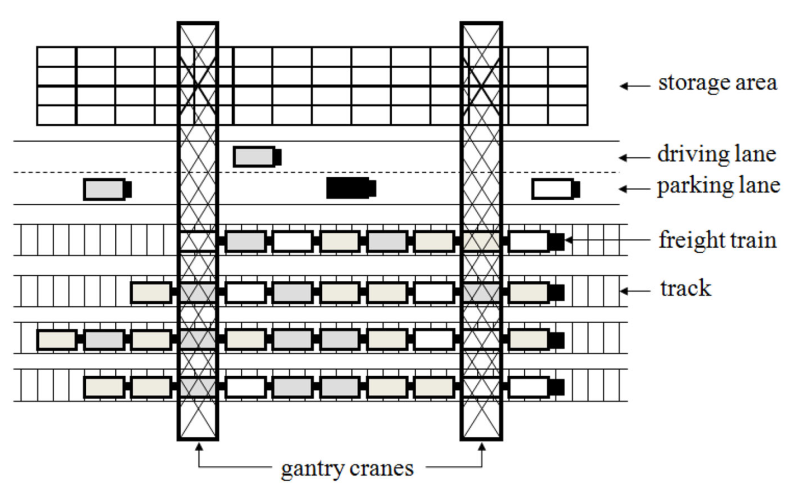
\includegraphics[width=0.9\textwidth]{img/costs.png}
\caption{\textsc{Schematische Darstellung eines Bahn-Terminals} \cite{Briskorn2018}.}
\label{fig:costs}
\end{figure}

\vfill
\pagebreak

Die Transportkosten werden in einer Matrix $C = (c_{iq})_{n \times m}$ kodiert,
wobei $c_{iq} \coloneqq d(O_i, F_q)$, d.h. der Eintrag an der Stelle $c_{iq}$ entspricht
den Kosten für den Transport eines Items $i \in I$ in einen Stack $q \in Q$.
Die Zuweisung des Items $i$ zu den unterschiedlichen Leveln $l \in \{1, \dotsc, b\}$ innerhalb des Stacks $q$
verursacht stets dieselben Kosten.

\subsection{Nebenbedingungen}
\label{sec:constraints}

Bei der Lösung der in dieser Arbeit betrachteten Problemstellungen müssen, wie einleitend erwähnt,
neben der Kapazität der Stacks zwei weitere Kategorien von Nebenbedingungen berücksichtigt werden, welche in diesem Abschnitt
präzisiert werden. Zunächst geht es in Abschnitt \ref{sec:stacking_restrictions} um die Stacking-Constraints
und anschließend in Abschnitt \ref{sec:placement_restrictions} um die Placement-Constraints.

\subsubsection{Stacking-Constraints}
\label{sec:stacking_restrictions}

Es gibt in der Praxis vielfältige Gründe dafür, dass nicht jedes Item auf jedes andere Item gestapelt werden darf.
Aus diesen resultieren bestimmte Restriktionen, welche auch Teil der von \citet{Bruns2015} betrachteten Problemstellungen
sind und z.B. wie folgt lauten:
\begin{itemize}
  \item schwerere Items dürfen nicht auf leichteren Items platziert werden
  \item größere Items dürfen nicht auf kleineren Items platziert werden
  \item Items best. Materialien oder Zielorte dürfen nicht aufeinander gestapelt werden
\end{itemize}

All jene Restriktionen, welche unter der Bezeichnung Stacking-Constraints zusammengefasst werden,
werden in einer Binärmatrix $S = (s_{ij})_{n \times n}$ kodiert, wobei:
\[
    s_{ij} =
\begin{cases}
    1, & \text{wenn Item $i$ direkt auf Item $j$ gestapelt werden darf }\\
    0, & \text{sonst}
\end{cases}
\]

Diese Matrix lässt sich, wie in Abb. \ref{fig:matrix_to_graph} beispielhaft dargestellt, auch durch einen
gerichteten \textquote{Stacking-Graphen} $G^S = (I, A^S)$ repräsentieren, welcher eine Kante $(i, j) \in A^S$ enthält,
wenn $s_{ij} = 1$ gilt.
\begin{figure}[H]
  \begin{subfigure}[b]{0.5\textwidth}
  \centering
    $S =$
    $\left(
    \begin{array}{rrrr}
    0 & 1 & 1 & 0 \\
    1 & 0 & 1 & 0 \\
    1 & 0 & 0 & 0 \\
    1 & 1 & 1 & 0 \\
    \end{array} \right) $
    \caption{\textsc{Stacking-Matrix}}
    \label{fig:constraint_matrix}
  \end{subfigure}
  \hfill
  \begin{subfigure}[b]{0.5\textwidth}
  \centering
    \begin{tikzpicture}[->, scale=0.65, transform shape, node distance=2.5cm]
    \node[state] (A) {1};
    \node[state] (B) [right of=A] {2};
    \node[state] (C) [below of=A] {3};
    \node[state] (D) [right of=C] {4};

    \path (A) edge node {} (B)
          (A) edge node {} (C)

          (B) edge [bend right] node {} (A)
          (B) edge [bend left=10] node {} (C)

          (C) edge [bend left] node {} (A)

          (D) edge [bend left=10] node {} (A)
          (D) edge node {} (B)
          (D) edge node {} (C);
  \end{tikzpicture}
    \caption{\textsc{Stacking-Graph}}
    \label{fig:resulting_graph}
  \end{subfigure}
  \caption{\textsc{Repräsentation der Stacking-Constraints.}}
  \label{fig:matrix_to_graph}
\end{figure}

\vfill
\pagebreak

In dieser Arbeit werden ausschließlich transitive Stacking-Constraints betrachtet, d.h.
wenn $(i, j), (j, h) \in A^S$, dann gilt ebenfalls $(i, h) \in A^S$.
Diese Einschränkung ist auch in der Praxis zumeist gegeben, da die Stacking-Constraints häufig auf Eigenschaften wie dem Gewicht oder der Länge der Items basieren. Restriktionen dieser Art haben außerdem die besondere Eigenschaft, dass alle Items vergleichbar sind, d.h. für alle $i \neq j$ gilt $s_{ij} = 1$ oder $s_{ji} = 1$, was zur Folge hat,
dass eine totale Ordnung auf allen Items definiert wird (vgl. \citet{Bruns2015}).

Die Stacking-Constraints, welche in dieser Arbeit primär betrachtet werden, definieren jeweils partielle
Ordnungen auf der Menge der Items, weil die Relation zweier Items statt auf nur einer Eigenschaft,
z.B. auf dem Gewicht und der Länge der Items basiert und somit die totale Vergleichbarkeit,
also $\forall i, j \in I : i \leq j \lor j \leq i$, welche Voraussetzung einer totalen Ordnung ist, nicht gilt.
In Kapitel \ref{sec:test_data} wird das ebenfalls praktisch motivierte Verfahren, mit welchem die
Stacking-Constraints generiert werden, genau beschrieben.

\subsubsection{Placement-Constraints}
\label{sec:placement_restrictions}

Die unter der Bezeichnung Placement-Constraints zusammengefassten Einschränkungen bezüglich der Positionierung eines
Items resultieren z.B. aus der Länge oder dem Gewicht der Items und den entsprechenden Eigenschaften der Stacks. Es gibt allerdings auch Items mit speziellen Anforderungen, beispielsweise Kühlcontainer\footnote{Container, welche über eine elektrisch betriebene Kühleinheit verfügen.}, welche eine Energiequelle benötigen. Solche Items können nur Stacks mit entsprechender Konfiguration zugewiesen werden.

% Die Placement-Constraints sind durch Mengen $Q^i$ für die Items $i \in I$ gegeben, wobei $Q^i$
% der Menge der Stacks entspricht, denen Item $i$ zugewiesen werden kann, zu denen Item $i$ also kompatibel ist.
% Dieser Sachverhalt kann durch einen bipartiten Graph $G^P = (I \cup Q, E^P)$ modelliert werden, wobei
% eine Kante $\{i, q\} \in E^P$ angibt, dass Item $i \in I$ Stack $q \in Q$ zugewiesen werden kann.
% Diese Kanten können zusätzlich ein Gewicht erhalten, welches den Transportkosten $c_{iq}$ entspricht.
% Kanten, welche nicht existieren erhalten das Gewicht $\infty$.

Die Placement-Constraints werden indirekt über hohe Kostenwerte implementiert. Die Zuweisung eines Items zu einem
Stack, mit welchem es nicht kompatibel ist, verursacht folglich höhere Kosten als sämtliche zulässigen Zuweisungen.
Dies hat den Vorteil, dass es sich dabei initial nur um weiche Nebenbedingungen handelt,
d.h. es wird auch dann eine Lösung gefunden, wenn gegen diese Nebenbedingungen verstoßen wird.
Eine solche Lösung wird allerdings aufgrund des Kostenminimierungsansatzes nur in Fällen generiert,
in denen keine Lösung existiert, welche sämtliche Placement-Constraints respektiert.
Schließlich kann entschieden werden, ob solche Lösungen als zulässig gelten,
oder, ob die Placement-Constraints dessen ungeachtet als harte Nebenbedingungen und solche
Lösungen dementsprechend als unzulässig betrachtet werden.
Der wesentliche Grund der Entscheidung für diese Art der Implementation ist allerdings eher pragmatischer Natur, denn der in den konstruktiven Heuristiken, welche in Kapitel \ref{sec:constructive_heuristics} vorgestellt werden, verwendete Algorithmus zur Berechnung eines Minimum-Weight-Perfect-Matchings, erwartet einen vollständig bipartiten Graphen als Eingabe. Bei diesem Graphen handelt es sich um einen Kompatibilitätsgraphen, welcher Item-Tupel durch Kanten mit kompatiblen Stacks verbindet. Insofern muss jedes Item zunächst mit jedem Stack kompatibel sein. Da die Placement-Constraints genau dies jedoch verhindern, können diese nicht direkt durch ein Fehlen der entsprechenden Kanten umgesetzt werden.

\vfill
\pagebreak

Zunächst werden die Placement-Constraints in einer Binärmatrix $T = (t_{iq})_{n \times m}$ kodiert, wobei:
\[
    t_{iq} =
\begin{cases}
    1, & \text{wenn Item $i$ in Stack $q$ platziert werden darf }\\
    0, & \text{sonst}
\end{cases}
\]
Diese Matrix wird jedoch nicht direkt verwendet, um die Restriktionen zu implementieren. Stattdessen wird
die Transportkosten-Matrix $C = (c_{iq})_{n \times m}$, welche in Abschnitt \ref{sec:transport_costs} eingeführt wurde, nun wie folgt modifiziert:
\[
    c_{iq} =
\begin{cases}
    d(O_i, F_q), & \text{wenn $t_{iq} = 1$}\\
    \infty, & \text{sonst}
\end{cases}
\]
Der Eintrag an der Stelle $c_{iq}$ enthält also nur noch die tatsächlichen Transportkosten, wenn die
entsprechende Item-Stack-Zuweisung basierend auf den Placement-Constraints zulässig ist.
Ist dies nicht der Fall, so gilt $c_{iq} = \infty$.
Die Placement-Constraints gelten als verletzt, wenn eine Lösung eine Item-Stack-Zuweisung
der Kosten $\infty$ enthält.

\subsection{Komplexität}
\label{sec:complexity}

In den folgenden Kapiteln werden Stacking-Probleme mit Stacks der Kapazitäten $b = 2$
und $b = 3 $ betrachtet, welche besonders in Szenarien aus der Praxis, in denen es darum geht,
Container zu stapeln, von Interesse sind.

Wie \citet{Bruns2015} zeigten, handelt es sich bei dem Zulässigkeitsproblem mit einer Stack-Kapazität von $b=3$ und gegebenen transitiven Stacking-Constraints $s_{ij}$ um ein stark NP-vollständiges Problem. Erst kürzlich wurde zudem gezeigt, dass auch das Zulässigkeitsproblem mit einer Stack-Kapazität von $b=2$, gegebenen transitiven
Stacking-Constraints $s_{ij}$ und Placement-Constraints $t_{iq}$, NP-vollständig ist (vgl. \citet{Chernykh2019}).

Somit sind die in dieser Arbeit betrachteten Stacking-Probleme, bei welchen zusätzlich die Transportkosten minimiert
und jeweils Stacking- sowie Placement-Constraints berücksichtigt werden, ebenfalls NP-vollständig.
Deshalb werden im Folgenden effiziente heuristische Lösungsverfahren für diese Probleme präsentiert,
welche zum Ziel haben, bei möglichst geringer Laufzeit zu günstigen Ergebnissen zu gelangen.

\subsection{Zielfunktion}
\label{sec:objective}

Das Ziel, welches im Folgenden für sämtliche Problemstellungen angestrebt wird, ist eine günstige
Einlagerung sämtlicher Items, d.h. die Zielfunktion entspricht der Minimierung der Transportkosten.
Dabei haben Zulässigkeit und geringe Laufzeit Priorität. Eine Lösung wird als zulässig betrachtet,
wenn sämtliche Items unter Berücksichtigung der Stacking- und Placement-Constraints sowie der Stack-Kapazität,
eingelagert werden.

\vfill
\pagebreak

Der Fokus auf Zulässigkeit äußert sich darin, dass zunächst stets versucht wird, möglichst wenige der zur Verfügung stehenden Stacks zu verwenden, weshalb die Zielfunktion im Grunde zunächst darin besteht, die Anzahl der verwendeten Stacks zu minimieren bzw. die Anzahl der vollständig gefüllten Stacks zu maximieren, damit idealerweise jede Instanz zumindest zulässig gelöst wird.
Erst im Anschluss daran werden die Transportkosten minimiert.
Im Wesentlichen handelt es sich daher um eine Kombination zweier Zielfunktionen,
welche im Sinne der lexikographischen Optimierung mit eine Präferenzordnung ausgestattet sind.
Zu Beginn geht es darum, den zur Verfügung stehenden Platz in der Storage-Area durch initiales Generieren
möglichst vieler $b$-Tupel von Items, ökonomisch zu nutzen. Anschließend werden diese $b$-Tupel
zusammen mit den verbleibenden Items möglichst günstig den zur Verfügung stehenden Stacks zugewiesen.

Ein ausschließlicher Fokus auf Kostenminimierung, nachdem die Zulässigkeit erreicht ist, ist durch
einen Postprocessing-Schritt umsetzbar, in welchem zuletzt ausgewählte Items von den ihnen zugewiesenen Positionen
an andere, freie Positionen verschoben werden, sofern sich infolgedessen Kosten einsparen lassen.
Dafür stehen auch die bisher ungenutzten Stacks zur Verfügung.

Es kann in der Praxis durchaus sinnvoll sein, den zur Verfügung stehenden Platz ökonomisch zu nutzen
und nicht bedingungslos Kosten zu minimieren und dabei viele lediglich partiell gefüllte Stacks zu generieren.
Ebenso kann allerdings auch ein reiner Fokus auf Kostenminimierung erwünscht sein. Da sich für beide Varianten
entsprechende Szenarien aus der Praxis finden, stellen die konstruktiven Heuristiken,
welche in Kapitel \ref{sec:constructive_heuristics} vorgestellt werden, beide Varianten bereit.
Angesichts der primären Betrachtung der Transportkostenminimierung in dieser Arbeit,
wird der Postprocessing-Schritt in den Experimenten stets durchgeführt.

\vfill
\pagebreak

\section{Testdaten-Generierung}
\label{sec:test_data}

Um die im Zuge dieser Arbeit entwickelten Heuristiken testen, miteinander vergleichen
und bewerten zu können, galt es zunächst, möglichst realistische Instanzen von Stacking-Problemen
für die betrachteten Szenarien zu generieren.

\citet{Briskorn2018} haben einen Testdaten-Generator für verschiedene Szenarien entwickelt, bei denen
es darum geht, den Prozess zu simulieren, in welchem Kräne Container in einer Lagerfläche positionieren.
Dieser deckt unterschiedliche Ausgangssituationen ab, welche beispielsweise in Hafen-Containerterminals,
Lagerhallen und Bahnterminals auftreten.
Ein Großteil der zahlreichen Konfigurations- und Spezifikationsmöglichkeiten, die dieser
Generator bereitstellt, spielt für die in dieser Arbeit betrachteten Problemstellungen allerdings keine Rolle.
Es lassen sich dort Übergabepositionen, Bewegungseigenschaften für die Container, Daten zur Freigabe und Auslieferung von
Containern, Vorgängerlisten der Container basierend auf Auslieferungszeiten und viele weitere, in dieser Arbeit
ungenutzte Eigenschaften setzen, von denen viele verpflichtend sind. Die Regeln zur Generierung der Stacking-Constraints,
welche essenzieller Bestandteil jeder in dieser Arbeit betrachteten Instanz sind, sind dagegen nicht Teil des Generators.
Bei Verwendung dieses Generators müssten viele Eigenschaften spezifiziert werden, die in dieser Arbeit nicht
berücksichtigt werden und die generierten Instanzen enthielten dementsprechend zahlreiche ungenutzte Informationen,
weshalb es insgesamt sinnvoller ist, einen eigenen Testdaten-Generator zu implementieren, für die Generierung der
Stacking-Constraints hätte ohnehin auf eine eigene Implementation zurückgegriffen werden müssen.
Sollten in Zukunft weitere Aspekte einbezogen werden, welche von diesem Testdaten-Generator bereitgestellt
werden, wie z.B. Ein- und Auslagerungszeiten, so kann es ggf. zu einem späteren Zeitpunkt sinnvoll
sein, auf diesen zurückzugreifen. Zum jetzigen Zeitpunkt hält sich der Aufwand für eine eigene Implementation,
welche die Anforderungen der in dieser Arbeit betrachteten Szenarien besser abdeckt, in Grenzen und vermeidet den
erheblichen Overhead an ungenutzten Daten innerhalb der Instanzen.

Dieser zu Testzwecken entwickelte \textsc{TestDataGenerator} generiert unterschiedlich große Instanzen von Stacking-Problemen.
Die Größe einer Instanz bezieht sich dabei stets auf die Anzahl der betrachteten Items. Die Testinstanzen werden
in drei Kategorien unterteilt:
\begin{itemize}
  \item klein (\textbf{s}) ($\leq 100$ Items)
  \item mittelgroß (\textbf{m}) ($\approx 300$ Items)
  \item groß (\textbf{l}) ($\approx 500$ Items)\newline
  \vspace{-1\baselineskip}
\end{itemize}
Dabei handelt es sich um einen groben Rahmen, in welchem sich praktisch motivierte Container-Stacking-Probleme
typischerweise bewegen. Dieser findet sich auch in der Literatur wieder (vgl. \citet{Le2016}).

\vfill
\pagebreak

Der \textsc{TestDataGenerator} stellt zur Generierung der Test-Instanzen eine Reihe von Konfigurationsmöglichkeiten
bereit, welche im Folgenden vorgestellt werden. Um den Vergleichen eine gewisse Aussagekraft zu verleihen,
werden in den Experimenten pro Konfiguration $20$ Instanzen generiert.\newline

\textbf{Anzahl zur Verfügung stehender Stacks}

Die erste vom \textsc{TestDataGenerator} bereitgestellte Konfigurationsmöglichkeit ist der Spielraum $a$ in der Storage-Area, welcher der Anzahl der zusätzlichen Stacks entspricht, die über die Minimalanzahl hinausgeht.
Die Anzahl der Items $n$ sowie die Stack-Kapazität $b$ wird stets spezifiziert und in der Berechnung der Anzahl zur Verfügung stehender Stacks $m$ verwendet. Es werden mindestens $\ceil{\frac{n}{b}}$ Stacks benötigt, um sämtliche $n$ Items zuzuweisen.
Aufgrund der in Abschnitt \ref{sec:constraints} geschilderten Nebenbedingungen wären die meisten Instanzen bei dieser
Anzahl an Stacks jedoch unlösbar. Daher wird die Minimalanzahl der Stacks um $a$ erhöht und es gilt
$m = \ceil{\ceil{\frac{n}{b}} + a}$.\newline

\textbf{Stacking-Constraints}

Die zweite Möglichkeit der Konfiguration besteht in der Generierung der Stacking-Constraints,
von welcher zwei Varianten implementiert wurden, die jeweils spezifische Vor- und Nachteile aufweisen
und im \textsc{TestDataGenerator} ausgewählt werden können.\newline

\textbf{Variante 1}

Die Stacking-Matrix $S$ wird anhand einer definierten Wahrscheinlichkeit mit $1$- bzw. $0$-Einträgen gefüllt. Anschließend werden jene $1$-Einträge, welche aus Transitivität folgen, ergänzt.\newline

\textbf{Variante 2}

Für alle $n$ Items wird eine zufällige Länge und Breite generiert. Item $i \in I$ kann auf Item $j \in I$
platziert werden, wenn für dessen Länge $l_i$ und Breite $w_i$ gilt $l_i \leq l_j$ und $w_i \leq w_j$.
Zwei Items $i, j$ sind in beide Richtungen stapelbar, wenn $l_i = l_j$ und $w_i = w_j$ gilt.

Die zweite Variante erscheint realitätsnäher. Aufgrund der Tatsache, dass diese jedoch bei zufälligen Längen und
Breiten der Items stets zu einem Anteil von $1$-Einträgen in der Stacking-Matrix $S$ von ca. $25\%$ führt
und jener mit Variante 1 sehr gut konfigurierbar ist, kann Variante $1$ in Situationen zum Einsatz kommen,
in welchen eine solche Konfiguration erwünscht ist.

Die zu ungefähr einem Viertel mit $1$-Einträgen gefüllte Matrix $S$ ergibt sich bei partiellen Ordnungen der Dimension $2$,
die in der zweiten Variante der Stacking-Constraint-Generierung aufgrund der zwei Werte (Länge, Breite),
welche pro Item generiert werden, gegeben sind.
Diese partiellen Ordnungen lassen sich auch als Permutationen darstellen, wobei eine Kante zwischen
zwei Knoten im Vergleichbarkeitsgraphen existiert, wenn diese in der Permutation
vertauscht sind. Ein solches ungeordnetes Paar von Elementen einer Permutation wird auch Inversion
der Permutation genannt. Die erwartete Anzahl von Inversionen in zufälligen Permutationen
beträgt $\frac{n (n - 1)}{4}$ bzw. $\frac{1}{2} \binom{n}{2}$ (vgl. \citet{Heuberger2012}).
Eine Kante im Vergleichbarkeitsgraphen bedeutet in diesem Fall, dass die verbundenen Items
basierend auf Variante 2 der Stacking-Constraint-Generierung in mindestens einer Richtung stapelbar sind,
d.h. die erwartete Anzahl der Inversionen entspricht der erwarteten Anzahl an $1$-Einträgen in $S$.
Dies gilt im Allgemeinen für zufällige Längen und Breiten der Items und ist nicht zwingend der Fall,
wenn diese Werte jeweils aus kleineren Intervallen gewählt werden.\newline

\textbf{Placement-Constraints}

Die Placement-Constraints werden zufällig generiert, wobei die Wahrscheinlichkeit für $t_{iq} = 1$, also dafür,
dass ein Item $i \in I$ in einem Stack $q \in Q$ platziert werden darf, im \textsc{TestDataGenerator} konfiguriert werden kann.
In der Praxis sind tendenziell mehr Zuweisungen erlaubt als verboten.\newline

\textbf{Item- und Stackpositionierung}

Im Wesentlichen liegen der Item- und Stackpositionierung zwei Grids zugrunde. Zum einen die Storage-Area,
welche die Stacks beinhaltet und zum anderen die Fahrzeuge, auf welchen die Items geliefert werden.
Die Positionierung der Items und Stacks einer Instanz ist somit an die schematische Darstellung in Abb. \ref{fig:costs}
angelehnt. Daraus ergeben sich mehrere Konfigurationsmöglichkeiten, die unterschiedliche Auswirkungen haben
und durch den \textsc{TestDataGenerator} bereitgestellt werden.
In der Storage-Area existiert eine konfigurierbare Anzahl von Reihen, auf welche die Stacks verteilt werden.
Da die Grids nicht notwendigerweise direkt aneinander grenzen, sondern z.B. wie in Abb. \ref{fig:costs}
durch \textquote{Driving-} und \textquote{Parking-Lane} voneinander getrennt sind, kann zudem eine Distanz
zwischen der Storage-Area und dem zu entladenen Fahrzeug spezifiziert werden.
Ebenfalls konfigurierbar ist die Anzahl der Reihen im Grid, welches die initialen Item-Positionen $O_i$ repräsentiert.

Die Positionen der Items und Stacks sind jeweils durch $x$- und $y$-Koordinaten definiert,
welche sich aus der Länge und Breite der Zellen der beiden Grids ergeben, in welchen die Items platziert werden
bzw. bei ihrer Ankunft platziert sind. Diese Positionen werden gleichmäßig auf die zur Verfügung stehenden
Item- bzw. Stack-Reihen verteilt. Für die einzelnen Zellen wird eine einheitliche Größe angenommen,
welche sowohl für die Storage-Area, als auch für die Fahrzeuge gilt. Neben der Konfiguration der Anzahl der Reihen,
ist daher außerdem die Definition dieser Zellengröße der beiden Grids von Relevanz.
Die konkreten Maße der Items sind für deren Positionierung irrelevant und lediglich für
die zweite Variante der Stacking-Constraint-Generierung von Bedeutung.
Die Itemdimensionen haben dort direkten Einfluss auf die Stacking-Constraints,
weil beispielsweise die Wahrscheinlichkeit für Item-Paarungen, welche in beide Richtungen stapelbar sind,
mit steigenden Intervallgrößen, aus welchen die zufälligen Dimensionen gewählt werden, abnimmt.

\vfill
\pagebreak

Für eine Instanz mit $40$ Items und $17$ Stacks der Kapazität $b = 3$ ergibt sich bei
Zellendimensionen, welche sich am TEU\footnote{Twenty Foot Equivalent Unit (Standardcontainer).} orientieren,
mit einer konfigurierten Anzahl von drei Stackreihen,
zwei Itemreihen sowie einer Distanz zwischen Storage-Area und der ersten Fahrzeugspur vom Fünffachen
der Zellenbreite, die in Abb. \ref{fig:positioning_example} dargestellte Item- und Stackpositionierung.
Die Positionen entsprechen in der von oben betrachteten Darstellung in der Abbildung stets der unteren linken Ecke
eines Items bzw. Stacks.

\begin{figure}[H]
\centering
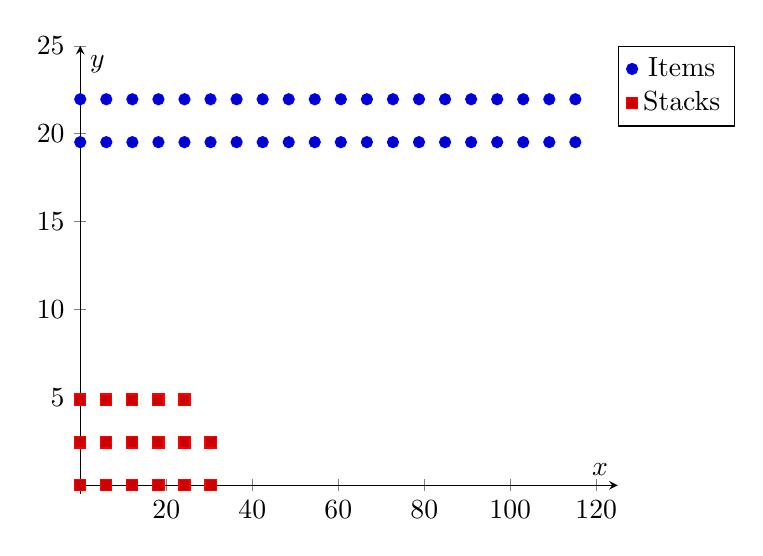
\begin{tikzpicture}
  \begin{axis}[
    axis lines=middle,
    xlabel=$x$,ylabel=$y$,
    xmin=-0.5,xmax=125.0,ymin=-0.5,ymax=25.0,
    legend style={at={(1,1)},anchor=north west}
    ]
    \addplot+[only marks] coordinates
    {
    (0.00,19.52) (6.06,19.52) (12.12,19.52) (18.18,19.52) (24.24,19.52) (30.30,19.52) (36.36,19.52) (42.42,19.52) (48.48,19.52) (54.54,19.52) (60.60,19.52) (66.66,19.52) (72.72,19.52) (78.78,19.52) (84.84,19.52) (90.90,19.52) (96.96,19.52) (103.02,19.52) (109.08,19.52) (115.14,19.52) (0.00,21.96) (6.06,21.96) (12.12,21.96) (18.18,21.96) (24.24,21.96) (30.30,21.96) (36.36,21.96) (42.42,21.96) (48.48,21.96) (54.54,21.96) (60.60,21.96) (66.66,21.96) (72.72,21.96) (78.78,21.96) (84.84,21.96) (90.90,21.96) (96.96,21.96) (103.02,21.96) (109.08,21.96) (115.14,21.96)
    };
    \addplot+[only marks] coordinates
    {
    (0.00,0.00) (6.06,0.00) (12.12,0.00) (18.18,0.00) (24.24,0.00) (30.30,0.00) (0.00,2.44) (6.06,2.44) (12.12,2.44) (18.18,2.44) (24.24,2.44) (30.30,2.44) (0.00,4.88) (6.06,4.88) (12.12,4.88) (18.18,4.88) (24.24,4.88)
    };
    \legend{Items, Stacks}
  \end{axis}
\end{tikzpicture}
\caption{\textsc{Beispiel für die Item- und Stackpositionierung.}}
\label{fig:positioning_example}
\end{figure}

\textbf{Transportkosten}

Die Kosten der Verladung eines Items in einen Stack entsprechen, wie in Abschnitt \ref{sec:transport_costs}
erläutert, der Distanz zwischen der Originalposition dieses Items und der Position des jeweiligen Stacks.
Zur Ermittlung der Distanzen zwischen Items und Stacks, werden deren Positionen bestehend aus
$x$- und $y$-Koordinaten, welche in zuvor beschriebener Weise generiert werden, herangezogen.
Die Metrik, welche der Distanzermittlung zu Grunde liegt, kann sich in unterschiedlichen Szenarien
unterscheiden und dementsprechend im \textsc{TestDataGenerator} definiert werden.

\vfill

%%%%%%%%%%%%%%%%%%%%%%%%%%%%%%%%%%%%%%%%%%%%%%%%%%%%%%%%%%%%%%%%%%%%%%%%%%%%%%%%%%%%%%%%%%%%%%%%%%%%
\pagebreak
%%%%%%%%%%%%%%%%%%%%%%%%%%%%%%%%%%%%%%%%%%%%%%%%%%%%%%%%%%%%%%%%%%%%%%%%%%%%%%%%%%%%%%%%%%%%%%%%%%%%

\section{MIP-Formulierungen}
\label{sec:mip_formulations}

In diesem Kapitel werden MIP-Formulierungen eingeführt, welche dem experimentellen Vergleich dienen.
Diese werden verwendet, um die optimalen Zielfunktionswerte der Test-Instanzen zu ermitteln und somit eine Grundlage zu schaffen, mit welcher die Qualität der von den Heuristiken generierten Lösungen beurteilt werden kann. Des Weiteren geht es um einen Vergleich der im Folgenden vorgestellten MIP-Formulierungen untereinander.
Es handelt sich dabei um auf die in dieser Arbeit betrachteten Problemstellungen angepasste Formulierungen,
welche in ihrer ursprünglichen Form von \citet{Le2016} vorgestellt wurden.
Zusätzlich zu eher marginalen Änderungen an den Nebenbedingungen, welche der etwas anderen Ausgangssituation geschuldet sind,
wird, wie bereits einleitend erwähnt, mit der Transportkostenminimierung jeweils eine andere Zielfunktion betrachtet.
In den ursprünglichen Formulierungen entspricht die Zielfunktion jeweils der Minimierung der Anzahl der verwendeten Stacks.

Die Zielfunktion der Heuristiken stellt, wie in Abschnitt \ref{sec:objective} geschildert, im Grunde die Kombination
zweier Zielfunktionen dar, welche initial die Anzahl der verwendeten Stacks minimiert, indem möglichst viele
$b$-Tupel von Items generiert werden, bevor diese möglichst günstig den Stacks zugewiesen werden.
Insofern ist zu erwarten, dass die MIP-Formulierungen verglichen mit den konstruktiven Heuristiken
aus Abschnitt \ref{sec:constructive_heuristics} prinzipiell, vorausgesetzt beide Lösungsverfahren lösen eine
Instanz zulässig, zu etwas günstigeren Zielfunktionswerten gelangen, dafür jedoch mehr Stacks verwenden.
Tatsächlich vergleichbar sind die Ergebnisse der MIP-Formulierungen mit jenen der Heuristiken allerdings nur,
wenn beide Lösungsverfahren dieselbe Zielfunktion betrachten. Dies wird durch ein Postprocessing-Verfahren
ermöglicht, welches beide konstruktiven Heuristiken bereitstellen und welches einen reinen Fokus auf die
Transportkostenminimierung ermöglicht, nachdem die Zulässigkeit erreicht ist.

Zunächst wird in Abschnitt \ref{sec:mip_definition} kurz die Idee der gemischt-ganzzahligen linearen Programmierung im Allgemeinen
eingeführt, um dann im Anschluss in den Abschnitten \ref{sec:bin_packing_formulation} und \ref{sec:three_idx_formulation} die beiden in dieser Arbeit betrachteten MIP-Formulierungen im Detail vorzustellen.

\subsection{Mixed Integer Linear Programming (MIP)}
\label{sec:mip_definition}

Viele kombinatorische Optimierungsprobleme lassen sich als lineare Programme formulieren, die sich dadurch
auszeichnen, dass die Zielfunktion eine lineare Funktion in Abhängigkeit von den Entscheidungsvariablen ist
und alle Nebenbedingungen in Form von linearen Gleichungen und Ungleichungen vorliegen. Für diese Probleme gibt es mit dem Simplexverfahren ein sehr effizientes Lösungsverfahren \cite{Knust2017}.

\vfill
\pagebreak

Ein gemischt-ganzzahliges lineares Programm (MIP) ist ein lineares Programm, welches kontinuierliche und ganzzahlige Variablen
enthält. Im Gegensatz zur kontinuierlichen Variante, ist die Lösung von ganzzahligen linearen Programmen NP-schwer.
Während sogar sehr große kontinuierliche lineare Programme durch kommerzielle Solver in wenigen Minuten gelöst werden können, gilt dies nicht für ganzzahlige lineare Programme. Diese können nur mit deutlich zeitaufwändigeren Algorithmen wie Branch \& Bound gelöst werden \cite{Brucker2006}.

In dieser Arbeit wird das Java-Interface von CPLEX, einem Solver für lineare Optimierungsprobleme verwendet,
um die MIP-Formulierungen, die in Abschnitt \ref{sec:bin_packing_formulation} und Abschnitt \ref{sec:three_idx_formulation} vorgestellt werden, zu lösen. Es handelt sich dabei um eine unter anderem auf dem Simplexverfahren basierende Implementation von IBM \cite{CPLEX2015}.

\subsection{Bin-Packing-Formulierung}
\label{sec:bin_packing_formulation}

Die Bin-Packing-Formulierung orientiert sich dem Namen nach am klassischen \textsc{Bin-Packing} Problem, bei dem es darum geht,
eine Menge von Objekten so auf eine Menge von Behältern zu verteilen, dass die Behälterkapazitäten eingehalten werden.
Wird dabei eine Lösung gesucht, die möglichst wenige Behälter verwendet, so handelt es sich um eines der klassischen NP-vollständigen
Probleme (vgl. \citet{Garey1979}).
Dies beschreibt auch direkt den Ansatz der Bin-Packing-Formulierung. Die Stacks werden als Behälter betrachtet und die Items als Objekte,
die diesen Behältern zugeordnet werden, wobei die Behälter- bzw. Stack-Kapazität jeweils eingehalten wird. Im Unterschied zum klassischen \textsc{Bin-Packing} müssen zusätzlich die Stacking- und Placement-Constraints berücksichtigt werden.

Es sei eine Menge von Items $I = \{1, \dotsc, n\}$ und eine Menge von Stacks $Q = \{1, \dotsc, m\}$ mit einer Kapazität von $b$ gegeben. Außerdem sei $G = (I, E)$ ein transitiver Stacking-Graph, welcher eine Kante $\{i, j\} \in E$ enthält,
wenn die entsprechenden Items $i, j \in I$ basierend auf den Stacking-Constraints in mindestens einer Richtung stapelbar sind,
d.h. wenn $s_{ij} + s_{ji} \geq 1$.
Bei den Variablen $x_{iq}$ handelt es sich um Binärvariablen, wobei $x_{iq} = 1$ bedeutet, dass Item $i$ Stack $q$ zugewiesen wird. Die Kosten werden über die Variablen $c_{iq}$ modelliert, wobei $c_{iq}$ den Kosten für den Transport des Items $i$ in den Stack $q$ entspricht.

Die Placement-Constraints werden implizit durch die Zielfunktion, welche die Transportkosten minimiert, berücksichtigt,
da diese, wie in Abschnitt \ref{sec:placement_restrictions} beschrieben, durch hohe Kostenwerte implementiert sind.
Es ist allerdings von Vorteil, diese in den MIP-Formulierungen explizit umzusetzen, weil sich dadurch kürzere
Laufzeiten erzielen lassen. Zu diesem Zweck seien die Placement-Constraints im Folgenden für jedes Item $i \in I$
durch die Menge $Q^i$ gegeben, wobei $Q^i$ der Menge an Stacks entspricht, denen Item $i$ basierend auf den Placement-Constraints zugewiesen werden darf, also sämtliche $q \in Q$, für die $t_{iq} = 1$ gilt.

\vfill
\pagebreak

% \begin{equation}
% \begin{aligned}
% & \text{min} & & \displaystyle\sum\limits_{i \in I}^{}\sum\limits_{q \in Q}^{} c_{iq} x_{iq} \\
% & \text{s.t.} & & \displaystyle\sum\limits_{q \in Q^i} x_{iq} = 1 & \forall i \in I\\
% &  & & \displaystyle\sum\limits_{i \in I} x_{iq} \leq b & \forall q \in Q\\
% \end{aligned}
% \end{equation}

% \begin{equation}
% \begin{array}{ll@{}ll}
% \text{minimize}   & \displaystyle\sum\limits_{i \in I}^{}\sum\limits_{q \in Q}^{} c_{iq} x_{iq} &\\
% \text{s.t.}       & \displaystyle\sum\limits_{q \in Q^i} x_{iq} = 1 & & \forall i \in I\\
%                   & \displaystyle\sum\limits_{i \in I} x_{iq} \leq b & & \forall q \in Q\\
% \end{array}
% \end{equation}

\begin{gather}
\boldsymbol{min} \quad \sum_{i \in I} \sum_{q \in Q} c_{iq} x_{iq} \label{bin_packing_line_one} \\
\thinspace\thinspace \boldsymbol{s.t.} \quad \quad \sum_{q \in Q^i} x_{iq} = 1 \quad\quad\quad\quad\quad\quad\quad \forall i \in I \quad\quad\quad\quad\thinspace\thinspace \label{bin_packing_line_two} \\
\thinspace \sum_{i \in I} x_{iq} \leq b \quad\quad\quad\quad\quad\quad\quad \forall q \in Q \label{bin_packing_line_three} \\
\thinspace\thinspace\quad\quad x_{iq} + x_{jq} \leq 1 \quad\quad\thinspace\thinspace\quad\quad\quad\quad \forall \{i, j\} \notin E \label{bin_packing_line_four} \\
\thinspace\thinspace\quad\quad\quad x_{iq} \in \{0, 1\} \thinspace\thinspace\thinspace\thinspace\thinspace\thinspace\quad\quad\quad\quad\quad\quad \forall i \in I, q \in Q \thinspace \label{bin_packing_line_five}
\end{gather}

In (\ref{bin_packing_line_one}) wird die betrachtete Zielfunktion definiert, welche die Summe der Kosten sämtlicher
Item-Stack-Zuweisungen minimiert, was der Minimierung der Transportkosten entspricht.
Nebenbedingung (\ref{bin_packing_line_two}) fordert, dass jedes Item genau einem Stack zugewiesen wird, mit welchem es kompatibel ist.
Die Ungleichung in (\ref{bin_packing_line_three}) entspricht der Forderung, dass für sämtliche Stacks die Stack-Kapazität eingehalten werden muss, d.h.
die Anzahl der eines Stacks zugewiesenen Items darf dessen Kapazität nicht überschreiten. (\ref{bin_packing_line_four}) entspricht schließlich der Forderung, dass alle Items, die nicht stapelbar sind, für die also keine Kante im Stacking-Graph existiert, nicht Teil desselben Stacks sind. (\ref{bin_packing_line_five}) definiert letztendlich die Domäne der Variablen $x_{iq}$.

Für diese MIP-Formulierung ist die Transitivität der Stacking-Constraints Voraussetzung, denn durch Nebenbedingung (\ref{bin_packing_line_four}) wird lediglich sichergestellt, dass die Items, welche gemeinsam in einem Stack platziert werden,
paarweise in einer Richtung stapelbar sind. Erst in Verbindung mit der Transitivität ergibt sich, dass auch für drei oder
mehr Items stets eine Reihenfolge existiert, in welcher diese innerhalb eines Stacks gestapelt werden dürfen.
Um diese Reihenfolge herzustellen, werden sämtliche Stacks, denen mehr als ein Item zugewiesen wurde, betrachtet. Für jeden
dieser Stacks wird geprüft, ob die aufeinander gestapelten Items jeweils paarweise aufeinander gestapelt sein dürfen.
Werden zwei Items innerhalb eines Stacks gefunden, welche die Stacking-Constraints verletzen, so werden diese
vertauscht und der Prozess startet für diesen Stack erneut. Ein vollständig gefüllter Stack mit $b = 3$ ist mit dieser
Strategie nach spätestens drei Tausch-Operationen korrekt sortiert. Da in dieser Arbeit lediglich Stack-Kapazitäten
von höchstens $b = 3$ betrachtet werden, ist dieses triviale Sortierverfahren ausreichend, für allgemeine $b$ sollte
hingegen ein effizienteres Verfahren verwendet werden.

\subsection{3-Index-Formulierung}
\label{sec:three_idx_formulation}

Die 3-Index-Formulierung enthält drei Indizes - Item, Stack und Level.
Im Gegensatz zur Bin-Packing-Formulierung, die Item-Stack-Zuweisungen vornimmt, weist die 3-Index-Formulierung einem
Item auch eine konkrete Position innerhalb eines Stacks zu, sie berücksichtigt also den Level.

\vfill
\pagebreak

Gegeben sei erneut eine Item-Menge $I = \{1, \dotsc, n\}$ und eine Stack-Menge $Q = \{1, \dotsc, m\}$, die Stacks der Kapazität $b$ enthält.
Jeder Stack enthält dementsprechend die Level $L = \{1, \dotsc, b\}$. Des Weiteren sei ein transitiver Stacking-Graph
$G = (I, A)$ gegeben, bei dem eine Kante $i \rightarrow j \in A$ bedeutet, dass das Item $i$ direkt auf das Item $j$ gestapelt werden darf.
Die Kosten seien durch die gegebene Transportkostenmatrix $C$ definiert, in der an der Stelle $c_{iq}$ die Kosten für den
Transport von Item $i$ in Stack $q$ stehen. Bei den Variablen $x_{iql}$ handelt es sich um Binärvariablen,
bei denen $x_{iql} = 1$ bedeutet, dass Item $i$ in Stack $q$ auf Level $l$ platziert wird. Wie bei der Bin-Packing-Formulierung
werden die Placement-Constraints auch hier explizit umgesetzt und die kompatiblen Stacks sind durch Mengen $Q^i$ für
alle Items $i \in I$ gegeben.

\begin{gather}
\boldsymbol{min} \quad \sum_{i \in I} \sum_{q \in Q} \sum_{l \in L} c_{iq} x_{iql} \label{three_idx_line_one} \\
\boldsymbol{s.t.} \quad \sum_{q \in Q^i} \sum_{l \in L} x_{iql} = 1 \quad\thinspace\thinspace\quad\quad\quad\quad \forall i \in I \thinspace\thinspace\quad\quad\quad\quad\quad\quad\quad\quad\thinspace\thinspace \label{three_idx_line_two} \\
\sum_{i \in I} x_{iql} \leq 1 \thinspace\quad\quad\quad\quad\quad\quad\quad \forall q \in Q, l \in L \thinspace\thinspace\thinspace\thinspace\quad\quad\quad\thinspace \label{three_idx_line_three} \\
\sum_{j \in I | i \rightarrow j \in A} x_{jq(l-1)} - x_{iql} \geq 0 \thinspace\quad\quad \forall i \in I, q \in Q, l \in L \textbackslash \{1\}
\label{three_idx_line_four} \\
\quad\quad x_{iql} \in \{0, 1\} \quad\quad\quad\quad\quad\quad\quad \forall i \in I, q \in Q, l \in L \quad\thinspace\thinspace\thinspace\thinspace\thinspace \label{three_idx_line_five}
\end{gather}

In (\ref{three_idx_line_one}) wird die Zielfunktion definiert, die erneut die Summe der Kosten sämtlicher Item-Zuweisungen
und somit die Transportkosten minimiert.
Nebenbedingung (\ref{three_idx_line_two}) fordert, dass sich jedes Item in genau einem kompatiblen Stack an genau
einer Position (Level) befindet,
also im Grunde, dass jedes Item einer Position in einem Stack zugewiesen wird.
Anschließend wird in (\ref{three_idx_line_three}) gefordert, dass sich an jeder Position in jedem Stack höchstens ein Item befindet und
(\ref{three_idx_line_four}) formuliert die Einschränkung, dass jedes Item, welches oberhalb des Ground-Levels platziert wird,
ein Item unter sich hat, welches sich basierend auf den Stacking-Constraints dort befinden darf.
Es setzt also die Stacking-Constraints um und sorgt zusätzlich dafür, dass kein Item \textquote{in der Luft} gestapelt wird.
Schließlich wird in (\ref{three_idx_line_five}) die Domäne der Variablen $x_{iql}$ definiert.

Beide Formulierungen weisen jedem Item einen Stack zu und minimieren dabei die Transportkosten.
Die Bin-Packing-Formulierung nimmt dabei lediglich Item-Stack-Zuweisungen vor, während die 3-Index-Formulierung die
Items konkreten Positionen innerhalb der Stacks zuweist. Dabei ist allerdings auch bei der Bin-Packing-Formulierung
sichergestellt, dass eine Item-Stack-Zuweisung nur dann vorgenommen wird, wenn die Items innerhalb des Stacks anschließend
in einer Weise umsortiert werden können, dass sie den Stacking Constraints entsprechen. Diese Tatsache ergibt sich aus Nebenbedingung (\ref{bin_packing_line_four}), welche fordert, dass Items sich nur dann im selben Stack befinden, wenn sie in mindestens einer Richtung stapelbar sind.
Da die Stacking Constraints außerdem transitiv sind, ist sichergestellt, dass die Reihenfolge innerhalb der Stacks stets so korrigiert werden kann, dass eine valide Lösung, welche die Stacking Constraints respektiert, dabei herauskommt.
Die 3-Index-Formulierung liefert folglich direkt eine zulässige Lösung, während die Item-Stack-Zuweisungen, welche die Bin-Packing-Formulierung liefert, zunächst noch sortiert werden müssen, damit sie eine zulässige Lösung ergeben.

\vfill
\pagebreak

\section{Untere Schranken}
\label{sec:lower_bounds}

Zur Abschätzung der Güte heuristischer Lösungen berechnet man bei Minimierungsproblemen häufig untere Schranken,
d.h. Werte $LB$, sodass $c(S) \geq LB$ für alle Lösungen $S$ gilt, wobei $c(S)$ dem Zielfunktionswert von $S$ entspricht.
Zur Berechnung solcher Schranken betrachtet man sogenannte Relaxationen\footnote{Einfachere Probleme, bei denen bestimmte Nebenbedingungen vernachlässigt werden.} des ursprünglichen Problems.
Da die Lösungsmenge des ursprünglichen Problems eine Teilmenge der Lösungsmenge der Relaxation ist,
definiert der optimale Zielfunktionswert der Relaxation eine untere Schranke für die optimale Lösung des Ausgangsproblems
\cite{Knust2017}.

Eine Abschätzung der Güte heuristischer Lösungen durch eine untere Schranke ist z.B. bei großen Instanzen hilfreich,
welche nicht bzw. nicht effizient durch die in Kapitel \ref{sec:mip_formulations} vorgestellten MIP-Formulierungen gelöst werden können.
Der optimale Lösungswert ist in solchen Fällen nicht bekannt, weshalb sich eine untere Schranke als Referenzwert
zur Beurteilung der Lösungsqualität heranziehen lässt. Eine untere Schranke für die Transportkosten einer Instanz eines Stacking-Problems lässt sich durch eine Relaxation des Problems bezüglich der Stacking-Constraints $s_{ij}$ generieren.
Die Placement-Constraints $t_{iq}$ sowie die Stack-Kapazität $b$ müssen weiterhin erfüllt werden.

Sei $P$ die Menge aller $mb$ Positionen innerhalb der Stacks und $q(p)$ jener Stack, zu welchem die Position $p$ gehört.
Ferner sei $G = (I \cup P, E)$ ein bipartiter Graph (siehe Abschnitt \ref{sec:digressions}), in welchem eine Kante $\{i, p\} \in E$ existiert, wenn $t_{iq(p)} = 1$, d.h. wenn ein Item $i \in I$ kompatibel zum Stack $q \in Q$ ist, zu welchem die Position $p$ gehört. Das Gewicht der Kante $\{i, p\}$ entspricht den Kosten $c_{iq(p)}$. Berechnet man nun ein
Minimum-Weight-Perfect-Matching (siehe Abschnitt \ref{sec:digressions}) in $G$, so entspricht das Gewicht des Matchings einer unteren Schranke für die Gesamtkosten.

\vfill
\pagebreak

\section{Konstruktive Heuristiken}
\label{sec:constructive_heuristics}

Bei den entwickelten konstruktiven Heuristiken handelt es sich um effiziente Lösungsverfahren für die in Kapitel \ref{sec:stacking_problems} beschriebenen Problemstellungen. Zunächst werden in Abschnitt \ref{sec:digressions} einige wichtige Konzepte eingeführt, welche in den Heuristiken Verwendung finden.
Anschließend geht es in Abschnitt \ref{sec:two_cap_heuristic} um eine konstruktive Heuristik für eine Stack-Kapazität
von $b = 2$ und darauffolgend, nach einem kurzen Abschnitt zur Konfiguration der Experimente in Abschnitt \ref{sec:experiments_config}, um einen experimentellen Vergleich der Solver für eben diese Stack-Kapazität in Bezug
auf die benötigten Laufzeiten und die Qualität der generierten Lösungen in Abschnitt \ref{sec:solver_comp_b=2}.
Abschnitt \ref{sec:three_cap_heuristic} behandelt eine konstruktive Heuristik für eine Stack-Kapazität von $b=3$, worauf erneut ein Vergleich der entsprechenden Solver in Abschnitt \ref{sec:solver_comp_b=3} folgt.

\subsection{Hintergrund}
\label{sec:digressions}

Zunächst werden mit bipartiten Graphen, Minimum-Weight-Perfect-Matchings, Maxi\-/mum-Cardinality-Matchings und Maximum-Weight-Bipartite-Matchings vier wichtige Konzepte eingeführt, welche in den Heuristiken zum Einsatz kommen.\newline

\textbf{Bipartiter Graph}

Ein Graph $G = (V, E)$ heißt bipartit (vgl. Abb. \ref{fig:digression_bipartite_graph}), wenn die Knotenmenge in zwei disjunkte Teilmengen zerfällt
$(V = S \cup T$ mit $S \cap T = \emptyset$), sodass jede Kante einen Knoten aus $S$ mit einem Knoten aus $T$ verbindet \cite{HochschuleDarmstadt}.\newline
Es lassen sich folgende Äquivalenzen festhalten \cite{Leighton2010}:
\begin{itemize}
  \item $G$ bipartit $\iff$ $G$ 2-färbbar
  \item $G$ bipartit $\iff$ keine Kreise ungerader Länge in $G$
\end{itemize}
In Abb. \ref{fig:digression_bipartite_graph} ist die 2-Färbbarkeit eines bipartiten Graphen, bei welcher die eine Teilmenge
in grün und die andere Teilmenge in rot gefärbt ist, visualisiert. Wie man sieht, existieren in solchen Graphen
ausschließlich Kanten, welche einen Knoten der einen Teilmenge (rot) mit einem Knoten der anderen Teilmenge (grün) verbinden,
jedoch keine Kanten zwischen Knoten derselben Farbe bzw. Teilmenge.

\begin{figure}[H]
\centering
\begin{tikzpicture}[scale=0.75, transform shape, node distance=3cm]
  \node[state] [mygreen] (A) {};
  \node[state] [red] (B) [above right of=A] {};
  \node[state] [mygreen] (C) [below right of=B] {};
  \node[state] [red] (D) [below of=B] {};
  \node[state] [red] (E) [below of=A] {};
  \node[state] [mygreen] (F) [right of=E] {};

  \path (A) edge node {} (B)
        (B) edge node {} (C)
        (C) edge node {} (D)
        (A) edge node {} (D)
        (A) edge node {} (E)
        (E) edge node {} (F)
        (D) edge node {} (F);

\end{tikzpicture}
\caption{\textsc{Bipartiter Graph.}}
\label{fig:digression_bipartite_graph}
\end{figure}

\vfill
\pagebreak

Ein Graph wird als vollständig bipartit bezeichnet, wenn jeder Knoten der einen Teilmenge mit jedem Knoten
der anderen Teilmenge durch eine Kante verbunden ist \cite{Knust2019}. Der in Abb. \ref{fig:digression_bipartite_graph}
dargestellte Graph ist dementsprechend nicht vollständig bipartit.\newline

\textbf{Minimum-Weight-Perfect-Matching (\textsc{MWPM})}

Gegeben sei ein ungerichteter Graph $G = (V, E)$. Eine Menge $M \subseteq E$ heißt Matching,
wenn keine zwei Kanten aus $M$ einen Knoten gemeinsam haben \cite{Gibbons1985}. Bei einem Matching handelt es sich also
um eine Menge unabhängiger Kanten. Ein Perfect-Matching ist wiederum ein Matching, in welchem jeder Knoten des Graphen
Endpunkt einer Kante des Matchings ist \cite{Gibbons1985} (vgl. Abb. \ref{fig:perfect_matching}).
Daher ist ein Perfect-Matching nur für Graphen mit einer geraden Anzahl an Knoten möglich.
In einem gewichteten Graphen ist ein Minimum-Weight-Matching ein Matching, bei welchem die Summe der Kantengewichte
minimal ist \cite{Gibbons1985}. Ein Minimum-Weight-Perfect-Matching ist dementsprechend ein günstigstes Perfect-Matching
basierend auf den Kantenkosten.

\begin{figure}[H]
\centering
\begin{tikzpicture}[-, scale=0.6, transform shape, node distance=3cm]
    \node[state] (A) {};
    \node[state] (B) [above right of=A] {};
    \node[state] (C) [below right of=A] {};
    \node[state] (D) [right of=B] {};
    \node[state] (E) [right of=D] {};
    \node[state] (F) [right of=C] {};

    \path (A) edge [red] node {} (B)
          (A) edge node {} (C)
          (B) edge node {} (D)
          (B) edge node {} (C)
          (D) edge [red] node {} (E)
          (D) edge node {} (F)
          (C) edge [red] node {} (F);
\end{tikzpicture}
\caption{\textsc{Perfect-Matching (dargestellt in rot).}}
\label{fig:perfect_matching}
\end{figure}

Der Algorithmus zur Berechnung von Minimum-Weight-Perfect-Matchings, welcher in den im Folgenden
vorgestellten Heuristiken zum Einsatz kommt, stammt aus der Java-Bibliothek \textsc{JGraphT} \cite{JGraphT}, trägt
den Namen \textit{KuhnMunkresMinimalWeightBipartitePerfectMatching} und ist eine Implementation der
sogenannten Ungarischen Methode zum Lösen von Zuordnungsproblemen in bipartiten Graphen.
Die Laufzeitkomplexität der Implementation beträgt $O(n^3)$, wobei $n$ der Anzahl der Knoten im Graphen entspricht.
Als Eingabe wird ein vollständig bipartiter Graph $G$ erwartet, d.h. $G= (S \cup T, E)$, wobei $S \cap T = \emptyset$ und
$\forall s \in S, t \in T \thinspace \exists \thinspace \{s, t\} \in E$. Außerdem wird erwartet, dass beide Partitionen gleich groß sind,
also $|S| = |T|$. Bei der Rückgabe des Algorithmus handelt es sich um ein Perfect-Matching der geringsten Kosten.\newline

\textbf{Maximum-Cardinality-Matching (MCM)}

Ein Maximum-Cardinality-Matching ist ein Matching, welches eine maximale Anzahl von Kanten enthält \cite{Gibbons1985}.
Es kann mehrere unterschiedliche \textsc{MCM}s in einem Graphen geben.
In Abb. \ref{fig:mcm_examples} sind beispielhaft zwei \textsc{MCM}s dargestellt.

\vfill
\pagebreak

\begin{figure}[H]
  \begin{subfigure}[b]{0.4\textwidth}
  \centering
    \begin{tikzpicture}[scale=0.6, transform shape, node distance=2cm]
    \node[state] (A) {};
    \node[state] (B) [above right of=A] {};
    \node[state] (C) [below left of=A] {};
    \node[state] (D) [below right of=C] {};
    \node[state] (F) [below right of=B] {};
    \node[state] (E) [below of=F] {};

    \path (A) edge [red] node {} (B)
          (A) edge node {} (C)
          (A) edge node {} (D)
          (A) edge node {} (E)
          (A) edge node {} (F)
          (C) edge [red] node {} (D);
  \end{tikzpicture}
  \caption{\textsc{$|MCM| = 2$}}
  \label{fig:mcm1}
  \end{subfigure}
  \hfill
  \begin{subfigure}[b]{0.4\textwidth}
  \centering
    \begin{tikzpicture}[scale=0.6, transform shape, node distance=2cm]
    \node[state] (A) {};
    \node[state] (B) [right of=A] {};
    \node[state] (C) [right of=B] {};
    \node[state] (D) [below left of=A] {};
    \node[state] (E) [below right of=D] {};
    \node[state] (F) [right of=E] {};

    \path (A) edge node {} (B)
          (B) edge [red] node {} (C)
          (B) edge node {} (F)
          (A) edge node {} (E)
          (E) edge [red] node {} (F)
          (A) edge [red] node {} (D)
          (D) edge node {} (E);
  \end{tikzpicture}
    \caption{\textsc{$|MCM| = 3$}}
    \label{fig:mcm_2}
  \end{subfigure}
  \caption{\textsc{MCMs (dargestellt in rot).}}
  \label{fig:mcm_examples}
\end{figure}

Der Algorithmus zur Berechnung von Maximum-Cardinality-Matchings, welcher in den im Folgenden
vorgestellten Heuristiken Anwendung findet, stammt ebenfalls aus der Java-Bibliothek \textsc{JGraphT} \cite{JGraphT} und trägt
den Namen \textit{EdmondsMaximumCardinalityMatching}. Es handelt sich dabei um eine Implementation von Edmonds' Blossom-Algorithmus,
welcher \textsc{MCM}s in ungerichteten Graphen berechnet. Der Algorithmus liefert ein Perfect-Matching, sofern eines existiert.
Andernfalls wird das größte Non-Perfect-Matching zurückgegeben.
Der Algorithmus besitzt eine Laufzeitkomplexität von $O(nm \thinspace \alpha(m, n))$, wobei $n$ der Anzahl der Knoten
und $m$ der Anzahl der Kanten im Graphen entspricht.\newline

\textbf{Maximum-Weight-Bipartite-Matching (MWBM)}

Bei einem Maximum-Weight-Bipartite-Matching handelt es sich um ein Matching in einem gewichteten bipartiten Graphen,
in welchem die Summe der Kantengewichte maximal ist. Auch diesen Algorithmus stellt \textsc{JGraphT} \cite{JGraphT}
unter dem Namen \textit{MaximumWeightBipartiteMatching} bereit.
Die Implementation besitzt eine Laufzeitkomplexität von $O(n (m + n \thinspace log \thinspace n))$, wobei $n$ der Knotenanzahl
und $m$ der Anzahl der Kanten im Graphen entspricht.

\subsection{Konstruktive Heuristik ($b = 2$)}
\label{sec:two_cap_heuristic}

Die konstruktive Heuristik zur Lösung von Stacking-Problemen mit Stacks der Kapazität $b=2$ erweitert den Ansatz aus dem Beweis
zu Theorem 1 aus der einleitend erwähnten Arbeit von \citet{Bruns2015}.

Zunächst wird ein Stacking-Graph $G = (V, E)$ generiert, welcher die Items als Knoten enthält, d.h. $V = I$. Dieser Graph
enthält eine Kante $\{i, j\} \in E$ zwischen zwei Knoten, wenn die entsprechenden Items $i, j \in I$ basierend auf den Stacking-Constraints
in mindestens einer Richtung stapelbar sind, d.h. wenn $s_{ij} + s_{ji} \geq 1$ und wenn mindestens ein Stack existiert, in welchem die beiden Items gemeinsam platziert werden können ohne die Placement-Constraints zu verletzen, also wenn $c_{iq} < \infty$ und $c_{jq} < \infty$ für
mindestens einen Stack $q \in Q$ gilt.

Berechnet man nun ein \textsc{MCM} in $G$ und interpretiert dessen Kanten als Stacks, welche die beiden Knoten, die durch
die Kanten verbunden werden, als Items enthalten, so erhält man eine größtmögliche Anzahl an vollständig gefüllten Stacks.
Items, welche nicht inzident zu einer Kante des Matchings sind, werden auf dem Ground-Level eines eigenen Stacks platziert.
Insgesamt werden auf diese Weise so wenig Stacks wie möglich verwendet, denn auch wenn der eigentliche Gegenstand der Optimierung die Transportkosten sind, steht zunächst stets im Vordergrund, überhaupt eine zulässige Lösung zu finden, weshalb die Maximierung der Anzahl der vollständig gefüllten Stacks initial eine gute Strategie darstellt.
Eine zulässige Lösung mit maximal $m$ Stacks kann nur dann existieren, wenn die Anzahl der Kanten im Matching und die Anzahl der nicht gematchten Knoten in der Summe nicht größer ist als $m$.

Aufgrund der Placement-Constraints kann allerdings nicht jedes Item in jedem Stack platziert werden, weshalb noch eine bestmögliche Zuweisung von Items und Item-Paaren zu Stacks gefunden werden muss. Diese entspricht einer Zuweisung, in welcher sämtliche Items möglichst günstig einem kompatiblen Stack zugeordnet werden. Dazu wird ein bipartiter Graph $G_1 = (V_1 \cup V_2, A)$ eingeführt, dessen erste Partition $V_1$ die Items bestehend aus Item-Paaren und Unmatched-Items enthält, während die zweite Partition $V_2$ die zur Verfügung stehenden Stacks beinhaltet.
Eine Kante in $A$, welche ein Item $i \in V_1$ oder ein Item-Paar $(i, j) \in V_1$ mit einem Stack $q \in V_2$ verbindet, gibt an, dass das entsprechende Item $i$ bzw. Item-Paar $(i, j)$ dem jeweiligen Stack $q$ zugeordnet werden kann. Da die Placement-Constraints nicht direkt durch ein Fehlen der entsprechenden Kante in $G_1$, sondern indirekt durch ein hohes Gewicht ebendieser Kante umgesetzt werden, existieren Kanten zwischen sämtlichen Knoten
aus $V_1$ und denen aus $V_2$, also $\forall i \in V_1, q \in V_2 \thinspace \exists \thinspace \{i, q\} \in A$.
Das Gewicht einer solchen Kante ist definiert als die Kosten $c_{iq}$ des Transports des Items $i$ von seiner Originalposition $O_i$ auf dem Fahrzeug, mit welchem es geliefert wird, zum Stack $q$
in der Storage-Area. Im Fall eines Item-Paars $(i, j) \in V_1$ entspricht das
Gewicht der Kante $\{(i, j), q\} \in A$ der Summe der Kosten des Transports beider Items, also $c_{(i, j)q} = c_{iq} + c_{jq}$.

Da der von \textsc{JGraphT} bereitgestellte Algorithmus, welcher zur Berechnung eines \textsc{MWPM} in $G_1$ verwendet wird,
einen vollständig bipartiten Graphen, dessen Partitionen dieselbe Größe besitzen, als Eingabe erwartet und die Summe der Items und Item-Paare
nicht notwendigerweise der Anzahl der verfügbaren Stacks entspricht, werden Dummy-Items eingeführt.
Diese Dummy-Items füllen $V_1$ für den Fall, dass diese Partition kleiner ist, auf.
Übersteigt die Anzahl der Items und Item-Paare die Anzahl der zur Verfügung stehenden Stacks, so existiert,
wie bereits erwähnt, ohnehin keine zulässige Lösung.
Die Dummy-Items haben keinen Einfluss auf die Lösung, da sämtliche Kanten, die ein Dummy-Item mit einem Stack verbinden,
das Gewicht $0$ besitzen und somit keine günstigere Zuweisung eines echten Items oder Item-Paars durch ein Dummy-Item
verhindert wird. Diese Tatsache ergibt sich daraus, dass die Dummy-Items jedem Stack zu den Kosten $0$ zugewiesen
werden können, während eine Zuweisung echter Items und Item-Paare stets Kosten verursacht. Dementsprechend werden
echte Items bei der Zuweisung gewissermaßen bevorzugt, während Dummy-Items schlicht den verbleibenden Stacks zugewiesen werden.

Nachdem beide Partitionen dieselbe Größe besitzen, wird ein \textsc{MWPM} in $G_1$ berechnet, dessen Kanten als
Stackzuweisungen interpretiert werden. Da es sich um ein Perfect-Matching handelt, werden sämtliche Items und Item-Paare einem Stack zugewiesen. Die Minimum-Weight-Variante eines Perfect-Matchings sorgt dafür, dass es sich um eine günstigste Zuweisung sämtlicher Items und Item-Paare zu Stacks handelt, da die Kantenkosten jeweils den Transportkosten der entsprechenden Items entsprechen. Sollte das \textsc{MWPM} eine Kante der Kosten $\infty$ enthalten, so existiert keine zulässige Zuweisung der generierten Item-Paare und Unmatched-Items zu den Stacks, welche die Placement-Constraints respektiert.

Abschließend muss ggf. die Reihenfolge der Items innerhalb der Stacks angepasst werden, da für die Item-Paare bisher nur sichergestellt ist, dass sie kompatibel und somit in mindestens einer Richtung stapelbar sind. Die Richtung, in welcher sie stapelbar sind, wurde bei der Zuweisung jedoch noch nicht berücksichtigt. Dies ist trivial möglich, indem für jene Stacks, welche ein Item-Paar beinhalten, überprüft wird, ob die Stacking-Constraints respektiert werden. Ist dies nicht der Fall, so werden die Items vertauscht. Anschließend ist garantiert, dass sämtliche Paare den Stacking-Constraints genügen.

Wie bereits in Abschnitt \ref{sec:objective} erwähnt, bietet die Heuristik über den Parameter
\textit{postProcessing} die Möglichkeit, einen Postprocessing-Schritt zu aktivieren, welcher einen reinen Fokus
auf die Transportkostenminimierung ermöglicht. Wird dieser Parameter auf \textit{true} gesetzt, so werden
ausgewählte Items von den ihnen zugewiesenen Positionen an andere, freie Positionen verschoben,
sofern sich dadurch eine Kostenersparnis ergibt. Diese Option sollte in Betracht gezogen werden,
wenn die Anzahl der verwendeten Stacks keine Rolle spielt und lediglich die entstehenden Transportkosten
von Relevanz sind.\newline

\textbf{Postprocessing-Schritt}

Zunächst wird ein bipartiter Postprocessing-Graph $G_p = (V_{p1} \cup V_{p2}, E_p)$ generiert, welcher die zuvor bereits platzierten Items $i \in I$ in der Partition $V_{p1}$ und die verbleibenden freien Positionen in den Stacks innerhalb der Storage-Area in der Partition $V_{p2}$ enthält. Eine solche Position entspricht einem Level $l \in \{1, \dotsc, b\}$ innerhalb eines Stacks $q \in Q$. Es existiert eine Kante $\{i, l\} \in E_p$ zwischen einem Item $i \in V_{p1}$ und einer freien Position $l \in V_{p2}$ innerhalb eines Stacks $q \in Q$, wenn das Item $i$ basierend auf den Placement-Constraints zu diesem Stack kompatibel ist, also wenn $t_{iq} = 1$ gilt. Zusätzlich muss das Item $i$ für den Fall, dass sich bereits ein Item $j \in I$ im Stack $q$ befindet, basierend auf den Stacking-Constraints mit diesem Item kompatibel sein, d.h. $s_{ij} = 1$ oder $s_{ji} = 1$.
Auf diese Weise kann nach der Zuweisung eines Items stets erneut eine den Stacking-Constraints entsprechende Anordnung innerhalb der Stacks erreicht werden. Die Kosten einer solchen Kante entsprechen der Kostenersparnis der Zuweisung des Items zum neuen Stack, verglichen mit den Kosten der gegenwärtigen Zuweisung dieses Items. Die Kostenersparnis $r_i$, welche sich bei der Zuweisung des Items $i \in I$, welches sich gegenwärtig im Stack $q_1 \in Q$ befindet, zum Stack $q$ ergibt, ist durch $r_i = c_{iq_1} - c_{iq}$ definiert. Eine Erhöhung der Kosten entspricht demnach einer negativen Ersparnis.

Daraufhin wird in $G_p$ ein Maximum-Weight-Bipartite-Matching berechnet, dessen Kanten jene Items mit freien
Positionen in den Stacks verbinden, welche zur insgesamt größten Kostenreduktion führen.
Dabei kann es vorkommen, dass einem zuvor leeren Stack zwei Items zugeordnet werden. Angesichts der Tatsache,
dass nicht gewährleistet ist, dass diese Items bezüglich der Stacking-Constraints miteinander kompatibel sind,
darf jedem Stack nur ein neues Item zugewiesen werden.
Es wird in solchen Fällen jenes Item mit der größeren Kostenersparnis verschoben.
Nachdem die Items an die ihnen zugeordneten Positionen verschoben wurden,
wird die Reihenfolge der Items innerhalb der Stacks, welchen ein zusätzliches Item zugewiesen
wurde ggf. basierend auf den Stacking-Constraints angepasst.
Befand sich ein verschobenes Item zuvor auf dem Ground-Level eines Stacks,
so wird das darüber platzierte Item auf den Ground-Level heruntergezogen,
sodass sich anschließend erneut eine zulässige Stacking-Lösung ergibt.
Dieser Postprocessing-Prozess wird iterativ durchgeführt, bis keine weitere Verringerung des Kostenwerts erzielt wird.\newline

\textbf{Beispiel}

Gegeben sei die Item-Menge $I = \{1, 2, 3, 4, 5, 6, 7\}$ sowie eine Stack-Kapazität von $b = 2$.
Die Anzahl der zur Verfügung stehenden Stacks wird nun, wie in Abschnitt \ref{sec:test_data} geschildert,
durch $m = \ceil{\ceil{\frac{n}{b}} + 0.2 \cdot \ceil{\frac{n}{b}}}$ berechnet und entspricht somit
$m = \ceil{\ceil{\frac{7}{2}} + 0.2 \cdot \ceil{\frac{7}{2}}} = 5$.
Die Stacking-Matrix $S$ wird ebenfalls, wie in Abschnitt \ref{sec:test_data} beschrieben, generiert.
Basierend auf dieser wird der in Abb. \ref{fig:stacking_const_graph_example_b=2_a} dargestellte Stacking-Graph
für die gegebenen Items eingeführt, auf welchem anschließend das in Abb. \ref{fig:stacking_const_graph_example_b=2_b} in grün dargestellte \textsc{MCM} berechnet wird. Das in rot dargestellte Item $5$ verbleibt dabei als einziges Unmatched-Item.

\begin{figure}[H]
  \centering
    \begin{subfigure}[b]{0.49\textwidth}
    \centering
    \begin{tikzpicture}[scale=0.7, transform shape, node distance=3cm]
        \node[state] (A) [thick] {$\boldsymbol{1}$};
        \node[state] (D) [thick, right of=A] {$\boldsymbol{4}$};
        \node[state] (E) [thick, below of=D] {$\boldsymbol{5}$};
        \node[state] (B) [thick, above of=D] {$\boldsymbol{2}$};
        \node[state] (C) [thick, below left = 1cm of E] {$\boldsymbol{3}$};
        \node[state] (F) [thick, below right = 1cm of E] {$\boldsymbol{6}$};
        \node[state] (G) [thick, right of=D] {$\boldsymbol{7}$};

        \path
            (A) edge [thick] node {} (B)
            (A) edge [thick] node {} (D)
            (A) edge [thick, bend right = 35] node {} (G)
            (A) edge [thick] node {} (E)
            (B) edge [thick, bend right = 75, distance=5.5cm] node {} (E)
            (B) edge [thick] node {} (D)
            (B) edge [thick] node {} (G)
            (C) edge [thick] node {} (F)
            (D) edge [thick] node {} (G)
            (E) edge [thick] node {} (G);
    \end{tikzpicture}
    \caption{\textsc{Stacking-Graph}}
    \label{fig:stacking_const_graph_example_b=2_a}
    \end{subfigure}
    % \hspace{em}
    \hfill
    \begin{subfigure}[b]{0.49\textwidth}
    \centering
    \begin{tikzpicture}[scale=0.7, transform shape, node distance=3cm]
        \node[state] (A) [thick] {$\boldsymbol{\textcolor{mygreen}{1}}$};
        \node[state] (D) [thick, right of=A] {$\boldsymbol{\textcolor{mygreen}{4}}$};
        \node[state] (E) [thick, below of=D] {$\boldsymbol{\textcolor{red}{5}}$};
        \node[state] (B) [thick, above of=D] {$\boldsymbol{\textcolor{mygreen}{2}}$};
        \node[state] (C) [thick, below left = 1cm of E] {$\boldsymbol{\textcolor{mygreen}{3}}$};
        \node[state] (F) [thick, below right = 1cm of E] {$\boldsymbol{\textcolor{mygreen}{6}}$};
        \node[state] (G) [thick, right of=D] {$\boldsymbol{\textcolor{mygreen}{7}}$};

        \path
            (A) edge [thick, mygreen] node {} (B)
            (A) edge [thick] node {} (D)
            (A) edge [thick, bend right = 35] node {} (G)
            (A) edge [thick] node {} (E)
            (B) edge [thick, bend right = 75, distance=5.5cm] node {} (E)
            (B) edge [thick] node {} (D)
            (B) edge [thick] node {} (G)
            (C) edge [thick, mygreen] node {} (F)
            (D) edge [thick, mygreen] node {} (G)
            (E) edge [thick] node {} (G);
    \end{tikzpicture}
    \caption{\textsc{MCM (Item $5$ unmatched)}}
    \label{fig:stacking_const_graph_example_b=2_b}
    \end{subfigure}
\caption{\textsc{Generierung der Item-Paare}.}
\label{fig:stacking_const_graph_example_b=2}
\end{figure}
Die Kanten des in Abb. \ref{fig:stacking_const_graph_example_b=2_b} in grün dargestellten \textsc{MCM} werden nun,
wie in Abb. \ref{fig:item_pairs_b=2} dargestellt, als kompatible Item-Paare interpretiert. Das als unmatched verbleibende
Item $5$ wird im Folgenden dem Ground-Level eines eigenen Stacks zugewiesen.
\begin{figure}[H]
\centering
\begin{tikzpicture}[scale=0.7, transform shape, node distance=3cm, state/.style={circle, draw, minimum size=1.25cm}]
        \node[state] (A) [thick] {\textcolor{mygreen}{$\boldsymbol{1, 2}$}};
        \node[state] (B) [thick, right of=A] {\textcolor{mygreen}{$\boldsymbol{3, 6}$}};
        \node[state] (C) [thick, right of=B] {\textcolor{mygreen}{$\boldsymbol{4, 7}$}};
        \node[state] (D) [thick, right of=C] {\textcolor{red}{$\boldsymbol{5}$}};
        \path ;
  \end{tikzpicture}
  \caption{\textsc{Resultierende Item-Paare.}}
  \label{fig:item_pairs_b=2}
\end{figure}

Nun geht es darum, eine möglichst günstige Zuweisung der Item-Paare und Unmatched-Items zu Stacks zu finden,
welche die Placement-Constraints respektiert. Dazu wird zunächst der vollständig bipartite Graph, welcher in
Abb. \ref{fig:bipartite_graph} dargestellt ist, generiert. Dieser enthält die Items bestehend aus Item-Paaren
und Unmatched-Items in der einen Partition und die Stacks in der anderen.
Da es lediglich $4$ Item-Tupel bei $5$ zur Verfügung stehenden Stacks gibt und damit die Partitionen nicht
dieselbe Größe besitzen, wird ein Dummy-Item $D_1$ eingeführt.
Die Kantengewichte sind der Übersichtlichkeit halber nicht in der Darstellung aufgetragen,
sondern stattdessen der Tabelle in Abb. \ref{fig:item_tuple_costs} zu entnehmen.

\begin{figure}[H]
\centering
\resizebox{0.5\textwidth}{!}{
\begin{tabular}{| c | c | c | c | c | c |}
    \hline
     & $\boldsymbol{S_1}$ & $\boldsymbol{S_2}$ & $\boldsymbol{S_3}$ & $\boldsymbol{S_4}$ & $\boldsymbol{S_5}$ \\ \hline
    $\boldsymbol{(1, 2)}$ & $\infty$ & $35.34$ & $47.46$ & $\infty$ & $71.7$ \\ \hline
    $\boldsymbol{(3, 6)}$ & $71.7$ & $59.58$ & $47.46$ & $47.46$ & $\infty$ \\ \hline
    $\boldsymbol{(4, 7)}$ & $\infty$ & $71.7$ & $59.58$ & $\infty$ & $47.46$ \\ \hline
    $\boldsymbol{5}$ & $38.88$ & $32.82$ & $26.76$ & $\infty$ & $\infty$ \\ \hline
    $\boldsymbol{D_1}$ & $0.0$ & $0.0$ & $0.0$ & $0.0$ & $0.0$ \\ \hline
\end{tabular}}
\caption{\textsc{Kosten der Stack-Zuweisungen}.}
\label{fig:item_tuple_costs}
\end{figure}

Anschließend wird im bipartiten Graphen aus Abb. \ref{fig:bipartite_graph} das \textsc{MWPM} berechnet,
welches in Abb. \ref{fig:mwpm_b=2} dargestellt ist. Jede Kante entspricht dabei der Zuweisung eines Item-Paars, Unmatched-Items
oder Dummy-Items zu einem Stack.

\begin{figure}[H]
\begin{subfigure}[b]{0.5\textwidth}
\centering
\begin{tikzpicture}[scale=0.7, transform shape, node distance=1.5cm, state/.style={circle, draw, minimum size=1.25cm}]
        \node[state] (A) [thick] {$\boldsymbol{1, 2}$};
        \node[state] (B) [thick, below of=A] {$\boldsymbol{3, 6}$};
        \node[state] (C) [thick, below of=B] {$\boldsymbol{4, 7}$};
        \node[state] (D) [thick, below of=C] {$\boldsymbol{5}$};
        \node[state] (E) [thick, below of=D] {$\boldsymbol{D_1}$};

        \node[state] (F) [thick, right = 4cm of A] {$\boldsymbol{S_1}$};
        \node[state] (G) [thick, right = 4cm of B] {$\boldsymbol{S_2}$};
        \node[state] (H) [thick, right = 4cm of C] {$\boldsymbol{S_3}$};
        \node[state] (I) [thick, right = 4cm of D] {$\boldsymbol{S_4}$};
        \node[state] (J) [thick, right = 4cm of E] {$\boldsymbol{S_5}$};

        \path
          % from (0,1) to all stacks
          (A) edge [thick] node {} (F)
          (A) edge [thick] node {} (G)
          (A) edge [thick] node {} (H)
          (A) edge [thick] node {} (I)
          (A) edge [thick] node {} (J)

          % from (2,5) to all stacks
          (B) edge [thick] node {} (F)
          (B) edge [thick] node {} (G)
          (B) edge [thick] node {} (H)
          (B) edge [thick] node {} (I)
          (B) edge [thick] node {} (J)

          % from (3,6) to all stacks
          (C) edge [thick] node {} (F)
          (C) edge [thick] node {} (G)
          (C) edge [thick] node {} (H)
          (C) edge [thick] node {} (I)
          (C) edge [thick] node {} (J)

          % from 4 to all stacks
          (D) edge [thick] node {} (F)
          (D) edge [thick] node {} (G)
          (D) edge [thick] node {} (H)
          (D) edge [thick] node {} (I)
          (D) edge [thick] node {} (J)

          % from dummy to all stacks
          (E) edge [thick] node {} (F)
          (E) edge [thick] node {} (G)
          (E) edge [thick] node {} (H)
          (E) edge [thick] node {} (I)
          (E) edge [thick] node {} (J);
  \end{tikzpicture}
  \caption{\textsc{Vollständig bipartiter Graph}}
  \label{fig:bipartite_graph}
\end{subfigure}
\hfill
\begin{subfigure}[b]{0.5\textwidth}
\centering
\begin{tikzpicture}[scale=0.7, transform shape, node distance=1.5cm, state/.style={circle, draw, minimum size=1.25cm}]
        \node[state] (A) [thick] {$\boldsymbol{1, 2}$};
        \node[state] (B) [thick, below of=A] {$\boldsymbol{3, 6}$};
        \node[state] (C) [thick, below of=B] {$\boldsymbol{4, 7}$};
        \node[state] (D) [thick, below of=C] {$\boldsymbol{5}$};
        \node[state] (E) [thick, below of=D] {$\boldsymbol{D_1}$};

        \node[state] (F) [thick, right = 4cm of A] {$\boldsymbol{S_1}$};
        \node[state] (G) [thick, right = 4cm of B] {$\boldsymbol{S_2}$};
        \node[state] (H) [thick, right = 4cm of C] {$\boldsymbol{S_3}$};
        \node[state] (I) [thick, right = 4cm of D] {$\boldsymbol{S_4}$};
        \node[state] (J) [thick, right = 4cm of E] {$\boldsymbol{S_5}$};

        \path
          (A) edge [thick, near start, above right] node {$35.34$} (G)
          (B) edge [thick, near start, above right] node {$47.46$} (I)
          (C) edge [thick, near end, below left] node {$47.46$} (J)
          (D) edge [thick, below right] node {$26.76$} (H)
          (E) edge [thick, near end, below right] node {$0.0$} (F);
  \end{tikzpicture}
  \caption{\textsc{MWPM}}
  \label{fig:mwpm_b=2}
\end{subfigure}
\caption{\textsc{Ermittlung der Stack-Zuweisungen minimaler Kosten}.}
\end{figure}

Sofern das in Abb. \ref{fig:mwpm_b=2} dargestellte \textsc{MWPM} keine Kante der Kosten $\infty$
enthält, handelt es sich um eine günstigste, zulässige Zuweisung sämtlicher Items und Item-Paare
zu Stacks. Andernfalls existiert keine solche Zuweisung für die gegebenen Paare und Unmatched-Items.
Im betrachteten Beispiel wurde demnach eine zulässige Lösung der Kosten $157.02$ gefunden.
Die entsprechende Interpretation des \textsc{MWPM} als zulässige Stack-Zuweisungen ist in Abb.
\ref{fig:stacking_solution} visualisiert.

\begin{figure}[H]
  \centering
  \resizebox{0.35\textwidth}{!}{
    \begin{tabular}{c|c|c|c|c|c|}
    \cline{2-6}
    $\boldsymbol{L_2}$ & $$ & $2$ & $$ & $6$ & $7$ \\ \cline{2-6}
    $\boldsymbol{L_1}$ & $$ & $1$ & $5$ & $3$ & $4$ \\ \cline{2-6}
    \multicolumn{1}{c}{} & \multicolumn{1}{c}{$\boldsymbol{S_1}$} & \multicolumn{1}{c}{$\boldsymbol{S_2}$}
    & \multicolumn{1}{c}{$\boldsymbol{S_3}$} & \multicolumn{1}{c}{$\boldsymbol{S_4}$} & \multicolumn{1}{c}{$\boldsymbol{S_5}$} \\
    \end{tabular}}
    \caption{\textsc{Zulässige Stack-Zuweisungen.}}
    \label{fig:stacking_solution}
\end{figure}

\vfill
\pagebreak

Zuletzt muss ggf. noch die Reihenfolge innerhalb der Stacks angepasst werden, da es sich bisher nur um zulässige Zuweisungen,
nicht aber um eine zulässige Ordnung der Items innerhalb der Stacks handelt.
Da jedoch sichergestellt ist, dass die Item-Paare kompatibel, d.h. in mindestens einer Richtung stapelbar sind,
ist dies trivial in der in Abschnitt \ref{sec:two_cap_heuristic} beschriebenen Weise möglich.

Ist der Postprocessing-Schritt aktiviert, so werden zuletzt ausgewählte Items an freie Positionen in anderen Stacks
verschoben, sofern sich dadurch eine Kostenersparnis ergibt. Dazu wird der bipartite Postprocessing-Graph generiert, welcher in
Abb. \ref{fig:post_processing_graph_two_cap} dargestellt ist. Dieser enthält die Items in der einen Partition
und die verbleibenden freien Positionen in der anderen Partition. Die Positionen sind jeweils in der Notation
$pos(stackIdx, level)$ gegeben.
In diesem Beispiel gibt es mit $pos(1, 1), pos(1, 2)$ und $pos(3, 2)$ drei verbleibende freie Positionen.
Da sämtliche Kantengewichte im Postprocessing-Graphen negativ oder neutral sind, kommt durch keine Verschiebung
eines Items eine Kostenersparnis zustande und es ist nicht möglich, die zuvor generierte Lösung im Postprocessing-Schritt zu
verbessern, weshalb die Zuweisungen aus Abb. \ref{fig:stacking_solution} unverändert bestehen bleiben.

\begin{figure}[H]
\centering
\begin{tikzpicture}[scale=0.5, transform shape, node distance=2.5cm, state/.style={circle, draw, minimum size=2cm}]
        \node[state] (A) [thick] {$\boldsymbol{1}$};
        \node[state] (B) [thick, below of=A] {$\boldsymbol{2}$};
        \node[state] (C) [thick, below of=B] {$\boldsymbol{3}$};
        \node[state] (D) [thick, below of=C] {$\boldsymbol{4}$};
        \node[state] (E) [thick, below of=D] {$\boldsymbol{5}$};
        \node[state] (F) [thick, below of=E] {$\boldsymbol{6}$};
        \node[state] (G) [thick, below of=F] {$\boldsymbol{7}$};

        \node[state] (H) [thick, right = 8cm of B] {$\boldsymbol{pos(1, 1)}$};
        \node[state] (I) [thick, right = 8cm of D] {$\boldsymbol{pos(1, 2)}$};
        \node[state] (J) [thick, right = 8cm of F] {$\boldsymbol{pos(3, 2)}$};

        \path

            (A) edge [thick, very near start, above right] node {$-6.06$} (J)
            (B) edge [thick, near end, above] node {$-6.06$} (H)
            (B) edge [thick, very near end, above right] node {$-6.06$} (I)
            (B) edge [thick, very near end, below left] node {$-6.06$} (J)
            (C) edge [thick, above] node {$-6.06$} (H)
            (C) edge [thick, near end, below] node {$-6.06$} (I)
            (D) edge [thick, very near start, above left] node {$-12.12$} (H)
            (D) edge [thick, very near start, above] node {$-12.12$} (I)
            (E) edge [thick, very near start, above left] node {$-12.12$} (H)
            (E) edge [thick, above] node {$-12.12$} (I)
            (E) edge [thick, near end, below] node {$0.0$} (J)
            (F) edge [thick, very near end, below right] node {$-18.18$} (H)
            (F) edge [thick, very near start, below right] node {$-18.18$} (I)
            (G) edge [thick, above] node {$-12.12$} (J);
\end{tikzpicture}

\caption{\textsc{Postprocessing-Graph}.}
\label{fig:post_processing_graph_two_cap}
\end{figure}


\subsection{Konfiguration der Experimente}
\label{sec:experiments_config}

In Kapitel \ref{sec:test_data} werden zahlreiche Konfigurationsmöglichkeiten vorgestellt, die vom \textsc{TestDataGenerator}
bereitgestellt werden. In diesem Abschnitt werden die Konfigurationen vorgestellt, welche den in den Abschnitten
\ref{sec:solver_comp_b=2} und \ref{sec:solver_comp_b=3} vorgestellten Experimenten zu Grunde liegen.

Zunächst zur Anzahl der zur Verfügung stehenden Stacks. In den durchgeführten Experimenten wird ein durchaus geringer Spielraum von
zusätzlichen $20 \%$ betrachtet, also $a = 0.2 \cdot \ceil{\frac{n}{b}}$, welcher in weiteren Betrachtungen erhöht werden könnte.
Für die Stacking-Constraint-Generierung wird auf die zweite der beiden vorgestellten Varianten zurückgegriffen,
weil diese realitätsnäher erscheint. Die in den Experimenten betrachteten Intervalle, aus welchen die zufällig generierten
Item-Maße stammen, welche im Folgenden definiert werden, führen zu ca. $36\%$ $1$-Einträgen in $S$.
Bei Vergrößerung der Intervalle nähert sich dieser Wert dem beschrieben Erwartungswert von ca. $25\%$ an.
Da, wie bereits erwähnt, für die Placement-Constraints gilt, dass in der Praxis tendenziell mehr Item-Stack-Zuweisungen erlaubt
als verboten sind, beträgt die Wahrscheinlichkeit für $t_{iq} = 1$, also dafür, dass ein Item $i \in I$ in einem
Stack $q \in Q$ platziert werden darf, $70 \%$.

Besonders viele Konfigurationsmöglichkeiten bietet die Item- und Stackpositionierung.
Das Grid, welches die initialen Item-Positionen $O_i$ repräsentiert, besteht in den in dieser Arbeit betrachteten
Instanzen stets aus zwei Reihen, welche beispielsweise zwei nebeneinander stehende Fahrzeuge repräsentieren,
die simultan entladen werden. Da die Storage-Area in der Praxis häufig ebenfalls aus wenigen, langen Spuren besteht,
werden auch die Stacks stets auf zwei Reihen verteilt.
Der als erstes weltweit standardisierte Seecontainer ist der 20-Fuß-Container TEU, welcher bis heute
international als Maßeinheit gebräuchlich ist. Der TEU ist $6.06 \thinspace m$ lang, $2.44 \thinspace m$ breit
und $2.59 \thinspace m$ hoch \cite{ContainerBasis}.
In Orientierung am TEU betragen Länge und Breite einer Zelle in den beiden Grids $6.06 \thinspace m$ bzw.
$2.44 \thinspace m$. Außerdem lässt sich die Distanz zwischen der Storage-Area und den Fahrzeugen konfigurieren,
für welche jeweils das fünffache der Zellenbreite, also in diesem Fall $12.20 \thinspace m$ angenommen wird.

Bei den Längen und Breiten der Items selbst handelt es sich um zufällige Werte, welche nicht die Zellengröße überschreiten.
Die Länge eines Items wird dementsprechend zufällig aus dem Intervall $[1.0, 6.0]$ generiert während die Breite aus dem
Intervall $[1.0, 2.4]$ stammt. Da es typischerweise nur eine begrenzte Anzahl unterschiedlicher Item-Typen im selben Lager
gibt, werden nicht sämtliche Werte aus diesen Intervallen betrachtet, sondern lediglich in Schritten von $0.5$.
Folglich sind die Item-Längen $\{1.0, 1.5, 2.0, 2.5, 3.0, 3.5, 4.0, 4.5, 5.0, 5.5, 6.0\}$ und
die Item-Breiten $\{1.0, 1.5, 2.0\}$ möglich.

Zuletzt wird definiert, auf welcher Metrik die Distanzen zwischen Item- und Stackpositionen
basieren, die schließlich den Transportkosten entsprechen.
In den im Zuge dieser Arbeit durchgeführten Experimenten basieren diese Distanzen in Anlehnung an das Beispiel
aus Abschnitt \ref{sec:transport_costs} stets auf der Manhattan-Metrik, welche die Kranbewegung in geeigneter Weise repräsentiert. Die Kosten der Zuweisung eines Items zu einem Stack ergeben sich somit aus der Manhattan-Distanz zwischen Itemposition $O_i$ und zugewiesener Stack-Position $F_q$. Für die Transportkostenmatrix $C = (c_{iq})_{n \times m}$ gilt
daher $c_{iq} \coloneqq d_{man}(O_i, F_q)$.

\vfill
\pagebreak

\subsection{Vergleich der Solver für $b = 2$}
\label{sec:solver_comp_b=2}

In diesem Abschnitt werden die verschiedenen Solver für Instanzen von Stacking-Problemen mit einer Stack-Kapazität von $b=2$ miteinander verglichen. Die relevanten Kategorien sind dabei der im Folgenden als Instance-Coverage bezeichnete prozentuale Anteil an gelösten Instanzen pro Solver und Test-Instanz-Konfiguration, die Laufzeiten, der Anteil der Instanzen, welcher pro Solver optimal gelöst wird
sowie die jeweilige prozentuale Abweichung der ermittelten Zielfunktionswerte vom Optimum.

Die in Kapitel \ref{sec:mip_formulations} vorgestellten MIP-Formulierungen wurden mit dem Java-Interface von \textsc{CPLEX} 12.8.0 implementiert
und gelöst. Dabei wurde \textsc{CPLEX} über den Parameter \textit{CPX\_MIPEMPHASIS\_FEASIBILITY} so konfiguriert, dass die Zulässigkeit
Priorität vor der Optimalität hat \cite{IBM_DOC}.

\textsc{CPLEX} terminiert in der Standardkonfiguration mit einer gewissen Toleranz bezüglich des optimalen Zielfunktionswerts.
Dabei werden zwei Toleranzen unterschieden, die relative Optimalitätstoleranz, welche über den Parameter
\textit{CPX\_PARAM\_EPGAP} konfigurierbar ist und die absolute Optimalitätstoleranz, welche über den Parameter
\textit{CPX\_PARAM\_EPAGAP} definiert werden kann. \textsc{CPLEX} terminiert, wenn eines der beiden Kriterien erfüllt ist \cite{CPLEX2015}.
Damit beide MIP-Formulierungen stets dieselben optimalen Zielfunktionswerte ermitteln, werden in den folgenden
Experimenten beide Parameter auf $0$ gesetzt, d.h. \textsc{CPLEX} terminiert ausschließlich dann vor dem Zeitlimit,
wenn die exakte Optimallösung gefunden wurde. In den betrachteten Experimenten wurden die Laufzeiten nur marginal
von dieser Konfiguration beeinflusst.

Die in dieser Arbeit entwickelten Heuristiken wurden ebenfalls in der Programmiersprache Java implementiert.
Wie in Abschnitt \ref{sec:two_cap_heuristic} erläutert, stellt die Heuristik für eine Stack-Kapazität von $b = 2$,
welche in den folgenden Experimenten zum Einsatz kommt, einen über den Parameter \textit{postProcessing} konfigurierbaren
Postprocessing-Schritt bereit, welcher einen reinen Fokus auf die Kostenminimierung ermöglicht. Dieser Schritt wird
in den durchgeführten Experimenten stets aktiviert. Sämtliche Experimente wurden auf einem System mit Intel Core i5-8500 (6x 3.00GHz) Prozessor und 32 GB RAM durchgeführt.\newline

\textbf{Kleine Instanzen (s)}

Zunächst zum experimentellen Vergleich der Solver für in Kapitel \ref{sec:test_data} als klein definierte Instanzen,
bei denen es darum geht, $100$ eintreffende Items in die Storage-Area zu verladen.
Die Diagramme in Abb. \ref{fig:instance_cov_b=2_s} zeigen jeweils die Instance-Coverage der einzelnen Solver.
In Abb. \ref{fig:instance_cov_b=2_s_a} handelt es sich um den prozentualen Anteil der zulässig gelösten Instanzen pro Solver bei einem Zeitlimit von $0.25s$ pro Instanz, in Abb. \ref{fig:instance_cov_b=2_s_b} bei einem Zeitlimit von $0.5s$ pro Instanz und in Abb. \ref{fig:instance_cov_b=2_s_c} schließlich bei $1s$ pro Instanz.\newline
Auf der $y$-Achse ist jeweils der prozentuale Anteil der gelösten Instanzen aufgetragen und auf der $x$-Achse der jeweilige Solver. Bei der Bin-Packing- und der 3-Index-Formulierung handelt es sich um keine Solver im eigentlichen Sinne,
sondern um MIP-Formulierungen, welche von \textsc{CPLEX} als Solver gelöst werden.
Im Folgenden wird der Einfachheit halber jedoch immer von drei Solvern gesprochen, womit die von
\textsc{CPLEX} gelösten MIP-Formulierungen und die Heuristik gemeint sind.
Die Solver werden in den Diagrammen und Abbildungen im Folgenden stets als \textsc{BinP} (Bin-Packing),
\textsc{3Idx} (3-Index) und \textsc{2Cap} (Heuristik für $b = 2$) abgekürzt.
Wie bereits in Kapitel \ref{sec:test_data} erläutert, werden jeweils $20$ Instanzen pro Konfiguration betrachtet,
d.h. die im Folgenden betrachteten Ergebnisse basieren auf der Lösung von in diesem Fall $20$ kleinen Instanzen.

Wie man Abb. \ref{fig:instance_cov_b=2_s} entnehmen kann, findet die Heuristik bei allen betrachteten Zeitlimits für sämtliche Instanzen eine zulässige Lösung, während die Bin-Packing-Formulie\-/rung bei einem Zeitlimit von $0.25s$ noch überhaupt keine Instanz zulässig löst und die 3-Index-Formulierung bei diesem Zeitlimit auf eine Instance-Coverage von $80 \%$ kommt (vgl. Abb. \ref{fig:instance_cov_b=2_s_a}). Bei einem Zeitlimit von $0.5s$ löst neben der Heuristik auch die 3-Index-Formulierung sämtliche Instanzen zulässig, während die Bin-Packing-Formulierung dort lediglich eine Instanz zulässig löst (vgl. Abb. \ref{fig:instance_cov_b=2_s_b}). Beim letzten betrachteten Zeitlimit von $1s$ nähert sich schließlich auch die Bin-Packing-Formulierung einer vollständigen Instance-Coverage und löst $90 \%$ der Instanzen zulässig.\newline
Die wesentliche Erkenntnis aus Abb. \ref{fig:instance_cov_b=2_s} ist allerdings, dass sämtliche Instanzen bereits bei einem Zeitlimit von $0.5s$ zulässig von einer MIP-Formulierung gelöst werden, was darauf hindeutet, dass der Bedarf für eine Laufzeitverbesserung durch eine Heuristik in dieser Kategorie aus praktischer Perspektive eher gering sein dürfte.

\begin{figure}[H]
\centering

\begin{subfigure}[b]{0.3\textwidth}
\centering
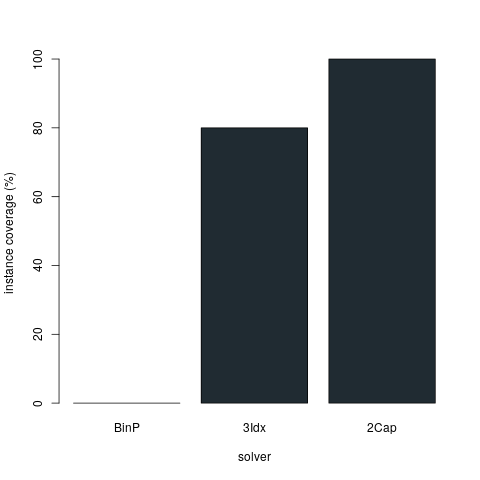
\includegraphics[width=1.1\textwidth]{img/solver_instance_coverage_b=2_s_0_25s.png}
\caption{\textsc{Zeitlimit $0.25s$}}
\label{fig:instance_cov_b=2_s_a}
\end{subfigure}
\hfill
\begin{subfigure}[b]{0.3\textwidth}
\centering
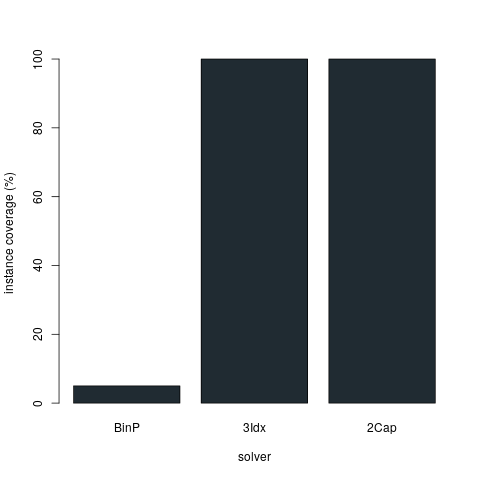
\includegraphics[width=1.1\textwidth]{img/solver_instance_coverage_b=2_s_0_5s.png}
\caption{\textsc{Zeitlimit $0.5s$}}
\label{fig:instance_cov_b=2_s_b}
\end{subfigure}
\hfill
\begin{subfigure}[b]{0.3\textwidth}
\centering
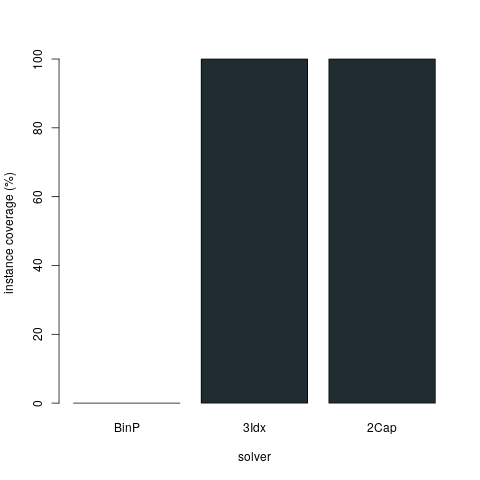
\includegraphics[width=1.1\textwidth]{img/solver_instance_coverage_b=2_s_1s.png}
\caption{\textsc{Zeitlimit $1s$}}
\label{fig:instance_cov_b=2_s_c}
\end{subfigure}

\caption{\textsc{Instance-Coverage der $b=2$ Solver (s)}.}
\label{fig:instance_cov_b=2_s}
\end{figure}

In Abb. \ref{fig:b=2_s_results} sind die Laufzeiten und ermittelten Zielfunktionswerte der Solver bei einem Zeitlimit von $1s$ dargestellt. Auf der $y$-Achse sind jeweils die gelösten Instanzen aufgetragen und auf der $x$-Achse die Laufzeiten bzw. ermittelten Kosten (Zielfunktionswerte). Für die Instanzen wird in sämtlichen Darstellungen die folgende Notation verwendet: (\textsc{items, stacks, capacity, index}). Abbildung \ref{fig:b=2_s_runtimes} zeigt die Laufzeiten der Solver pro Instanz in Sekunden bei einem Zeitlimit von $1s$.
Die 3-Index-Formulierung ist in der Regel deutlich schneller als die Bin-Packing-Formulierung und die Heuristik unterbietet beide MIP-Formulierungen noch einmal deutlich. Da in der Abbildung die absoluten Laufzeitdifferenzen zu sehen sind, ist es wichtig, zu erwähnen, dass die Laufzeiten der Heuristik durchschnittlich um den Faktor $24$ kleiner sind als jene der 3-Index-Formulierung. Zwischen der 3-Index- und der Bin-Packing-Formulierung besteht dagegen nur ein Faktor von $1.5$.

\vfill
\pagebreak

Aufgrund der Tatsache, dass \textsc{CPLEX} lediglich vor dem Zeitlimit terminiert, wenn die entsprechende Instanz optimal gelöst wird, ist klar ersichtlich, dass die 3-Index-Formulierung sämtliche Instanzen optimal löst (vgl. Abb. \ref{fig:b=2_s_runtimes}). Die Bin-Packing-Formu\-/lierung terminiert dagegen mit den Instanzen $00$ und $11$ in nur zwei Fällen vor dem Zeitlimit. Bei diesen handelt es sich um die einzigen Instanzen, welche optimal von der Bin-Packing-Formulierung gelöst werden, was daran erkennbar ist, dass die \textsc{BinP}-Einträge in der Darstellung der ermittelten Kosten durch die \textsc{3Idx}-Einträge verdeckt werden, weil beide Formulierungen denselben, optimalen Zielfunktionswert ermitteln (vgl. Abb. \ref{fig:b=2_s_costs}).
Sofern mehrere Solver denselben Wert ermitteln, verdecken sich die entsprechenden Einträge in der Reihenfolge, in welcher sie in der Legende aufgeführt sind. Dies gilt grundsätzlich für sämtliche Diagramme in den folgenden Experimenten.
Die Instanzen $03$ und $14$ werden von der Bin-Packing-Formulierung nicht einmal zulässig gelöst, was an den fehlenden
Einträgen zu erkennen ist (vgl. Abb. \ref{fig:b=2_s_runtimes}). Bei den $16$ verbleibenden Instanzen gelangt die Bin-Packing-Formulierung zu zulässigen Lösungen, die Zielfunktionswerte weichen allerdings, wie man Abb. \ref{fig:b=2_s_costs} entnehmen kann, deutlich von jenen der Heuristik und der 3-Index-Formulierung ab. Dabei ist zu beachten, dass die Darstellung in einer Weise skaliert wurde, welche es ermöglicht, sämtliche Einträge zu erkennen. Infolgedessen bildet diese nicht die tatsächlichen Abstände ab, welche anhand der Beschriftungen der $x$-Achse nachzuvollziehen sind.

Weiterhin ist zu sehen, dass die Heuristik in einigen Fällen deutlich näher an den Optimalwert herankommt als in anderen Fällen.
Bei Instanz $13$ wurde beispielsweise annähernd der Optimalwert ermittelt, während die Abweichung bei Instanz
$05$ erheblich größer ist. Insgesamt sind die Abweichungen allerdings mit deutlich unter einem Prozent in jedem
Fall sehr gering. Ferner sind unter der Abkürzung \textsc{LB\footnote{Lower Bounds}} jeweils die unteren Schranken dargestellt, welche in Abschnitt \ref{sec:lower_bounds} beschrieben werden. Diese zeigen den Einfluss der Stacking-Constraints auf die optimalen Zielfunktionswerte, welcher insgesamt eher gering zu sein scheint, wobei es auch hier Unterschiede zwischen den Instanzen gibt. Bei den Instanzen $07, 09$ und $10$ entspricht die untere Schranke dem optimalen Zielfunktionswert, was bedeutet, dass die Stacking-Constraints dort überhaupt keinen Einfluss auf den optimalen Zielfunktionswert haben.
In diesen Fällen überdecken die Einträge der 3-Index-Formulierung auch jene der unteren Schranken. Bei den Instanzen
$06$ und $17$ zeigt sich dagegen ein deutlich größerer Einfluss.

\vfill
\pagebreak

\begin{figure}[H]
\centering
\begin{subfigure}[b]{0.47\textwidth}
\centering
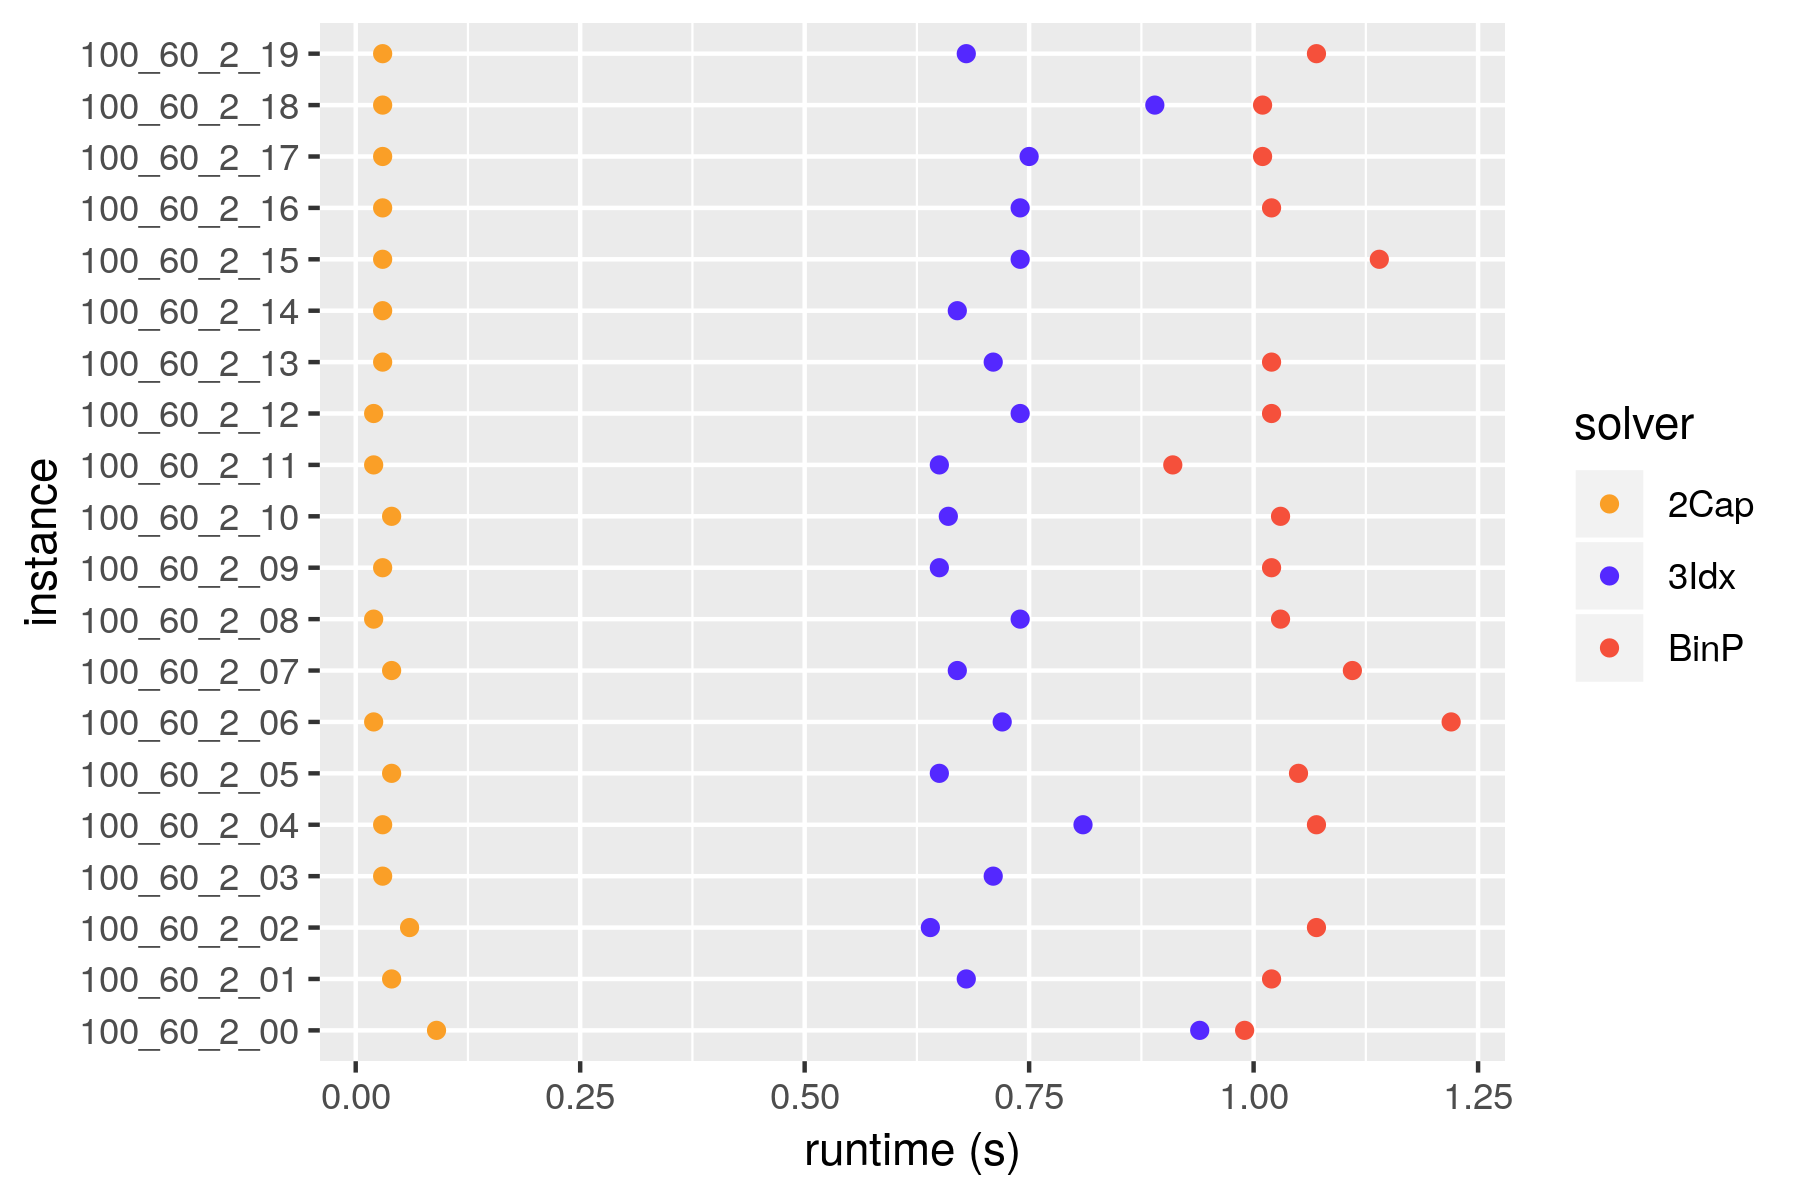
\includegraphics[width=1.1\textwidth]{img/solver_instance_time_b=2_s_1s.png}
\caption{\textsc{Laufzeiten}}
\label{fig:b=2_s_runtimes}
\end{subfigure}
\hfill
\begin{subfigure}[b]{0.47\textwidth}
\centering
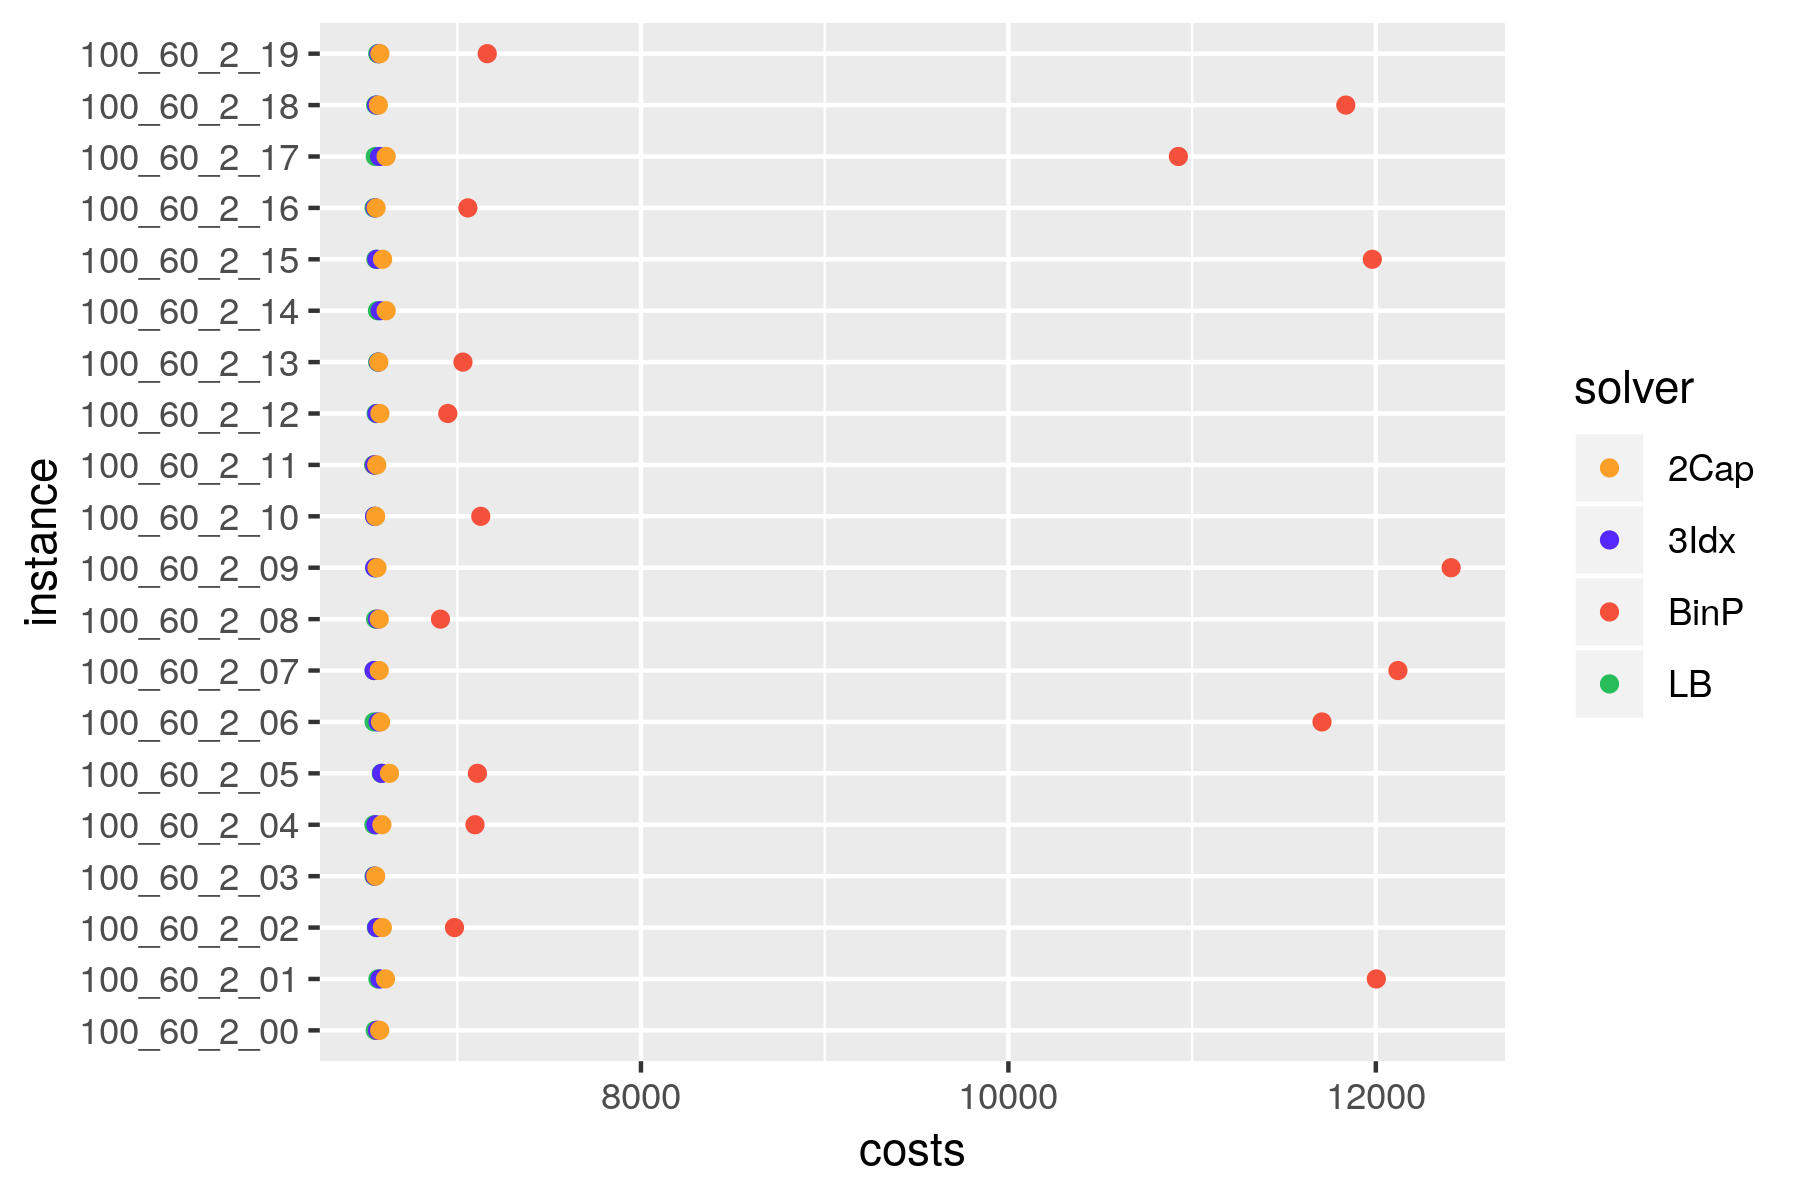
\includegraphics[width=1.1\textwidth]{img/solver_instance_cost_b=2_s_1s.png}
\caption{\textsc{Kosten}}
\label{fig:b=2_s_costs}
\end{subfigure}
\caption{\textsc{Ergebnisse bei $1s$ Zeitlimit}.}
\label{fig:b=2_s_results}
\end{figure}

Die exakten Ergebnisse der MIP-Formulierungen sind den Tabellen in Abb. \ref{fig:table} zu entnehmen.
\textquote{Optimal} bezeichnet den prozentualen Anteil der Instanzen, welcher optimal gelöst wurde.
Bei der Laufzeit handelt es sich um die durchschnittliche Laufzeit pro Instanz in Sekunden und die
Abweichung gibt die durchschnittliche prozentuale Abweichung vom optimalen Zielfunktionswert pro Instanz an.

\begin{figure}[H]
\centering

\begin{subfigure}[b]{0.3\textwidth}
\centering
\resizebox{\textwidth}{!}{
\begin{tabular}{ | c | c | c |}
    \hline
     & \textbf{BinP} & \textbf{3Idx} \\ \hline
    \textbf{Optimal ($\boldsymbol{\%}$)} & $ 0$ & $ 0$ \\ \hline
    \textbf{\O \thinspace Laufzeit ($\boldsymbol{s}$)} & $\textcolor{red}{-}$ & $\textcolor{mygreen}{0.26}$ \\ \hline
    \textbf{\O \thinspace Abweichung ($\boldsymbol{\%}$)} & $\textcolor{red}{-}$ & $\textcolor{mygreen}{34.22}$ \\ \hline
\end{tabular}}
\caption{\textsc{Zeitlimit} $0.25s$}
\label{fig:res_b=2_s_a}
\end{subfigure}
% $\quad\quad\quad\quad$
\begin{subfigure}[b]{0.3\textwidth}
\centering
\resizebox{\textwidth}{!}{
\begin{tabular}{ | c | c | c |}
    \hline
     & \textbf{BinP} & \textbf{3Idx} \\ \hline
    \textbf{Optimal ($\boldsymbol{\%}$)} & $ 0$ & $ 0$ \\ \hline
    \textbf{\O \thinspace Laufzeit ($\boldsymbol{s}$)} & $0.5$ & $0.5$ \\ \hline
    \textbf{\O \thinspace Abweichung ($\boldsymbol{\%}$)} & $\textcolor{red}{71.28}$ & $\textcolor{mygreen}{28.15}$ \\ \hline
\end{tabular}}
\caption{\textsc{Zeitlimit} $0.5s$}
\label{fig:res_b=2_s_b}
\end{subfigure}
% \end{figure}
% \begin{figure}[H]
\begin{subfigure}[b]{0.3\textwidth}
\centering
\resizebox{\textwidth}{!}{
\begin{tabular}{ | c | c | c |}
    \hline
     & \textbf{BinP} & \textbf{3Idx} \\ \hline
    \textbf{Optimal ($\boldsymbol{\%}$)} & $\textcolor{red}{10}$ & $\textcolor{mygreen}{100}$ \\ \hline
    \textbf{\O \thinspace Laufzeit ($\boldsymbol{s}$)} & $\textcolor{red}{1.05}$ & $\textcolor{mygreen}{0.72}$ \\ \hline
    \textbf{\O \thinspace Abweichung ($\boldsymbol{\%}$)} &$\textcolor{red}{35.03}$ & $\textcolor{mygreen}{0.0}$ \\ \hline
\end{tabular}}
\caption{\textsc{Zeitlimit} $1s$}
\label{fig:res_b=2_s_c}
\end{subfigure}

\caption{\textsc{MIP-Ergebnisse}.}
\label{fig:table}
\end{figure}

Abbildung \ref{fig:table} zeigt, dass die 3-Index-Formulierung der Bin-Packing-Formulierung in dieser Kategorie vorzuziehen ist,
da diese bei jedem betrachteten Zeitlimit zu besseren Ergebnissen gelangt und mit einer sehr geringen Laufzeit
von durchschnittlich $0.72s$ sämtliche Instanzen optimal löst. Bei einem Zeitlimit von $1s$ löst die Bin-Packing-Formulierung trotz einer Instance-Coverage von $90 \%$ nur $10 \%$ der Instanzen optimal und weicht im Durchschnitt erheblich vom Optimum ab (vgl. Abb. \ref{fig:res_b=2_s_c}).
Allerdings ist auch die 3-Index-Formulierung erst ab dem betrachteten Zeitlimit von $1s$ sinnvoll einsetzbar,
da diese bei den kleineren Zeitlimits im Durchschnitt ebenfalls deutlich vom Optimum abweicht.

Da die Zeitlimits aufgrund ihrer geringen Laufzeit für die Heuristik keine Rolle spielen, kommt diese stets zum selben Ergebnis. Sie weicht durchschnittlich um $0.29 \%$ vom Optimum ab und benötigt dafür eine durchschnittliche Laufzeit von nur $0.04s$.
Trotz dieser sehr guten Ergebnisse der Heuristik besteht aufgrund der Tatsache, dass die 3-Index-Formulierung sämtliche Instanzen
mit einer durchschnittlichen Laufzeit von $0.72s$ optimal löst, aus praktischer Perspektive vermutlich kein großer Bedarf für
eine Laufzeitverbesserung durch eine Heuristik.

\vfill
\pagebreak

\textbf{Mittelgroße Instanzen (m)}

Interessanter wird es bereits beim Vergleich der Solver für in Kapitel \ref{sec:test_data} als mittelgroß bezeichnete Instanzen,
bei denen es darum geht, $300$ eintreffende Items in die Storage-Area zu verladen.
In Abb. \ref{fig:instance_cov_b=2} ist erneut die Instance-Coverage der einzelnen Solver dargestelllt.

Bei einem Zeitlimit von $30s$ pro Instanz löst die Bin-Packing-Formulierung keine Instanz zulässig, während die 3-Index-Formulierung bereits für sämtliche Instanzen eine zulässige Lösung findet (vgl. Abb. \ref{fig:instance_cov_b=2_m_a}).
Selbiges gilt für das verdoppelte Zeitlimit von einer Minute (vgl. Abb. \ref{fig:instance_cov_b=2_m_b}). Bei einer weiteren
Verdopplung des Zeitlimits auf zwei Minuten, erreicht schließlich auch die Bin-Packing-Formulierung eine vollständige Instance-Coverage (vgl. Abb. \ref{fig:instance_cov_b=2_m_c}). Die Heuristik ist, wie zuvor, aufgrund ihrer geringen Laufzeiten
in keinem Fall vom Zeitlimit betroffen und löst daher in jedem Fall sämtliche Instanzen zulässig.

\begin{figure}[H]
\centering

\begin{subfigure}[b]{0.3\textwidth}
\centering
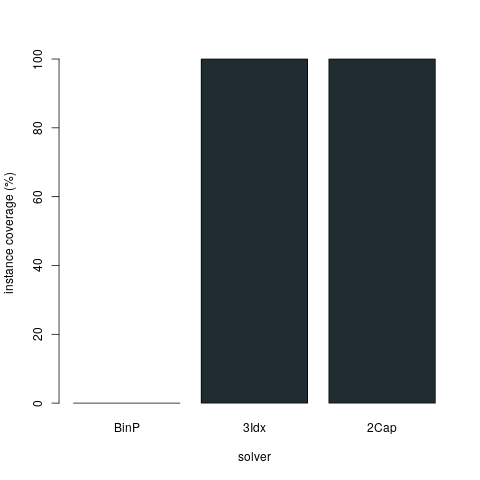
\includegraphics[width=1.1\textwidth]{img/solver_instance_coverage_b=2_m_30s.png}
\caption{\textsc{Zeitlimit} $30s$}
\label{fig:instance_cov_b=2_m_a}
\end{subfigure}
\hfill
\begin{subfigure}[b]{0.3\textwidth}
\centering
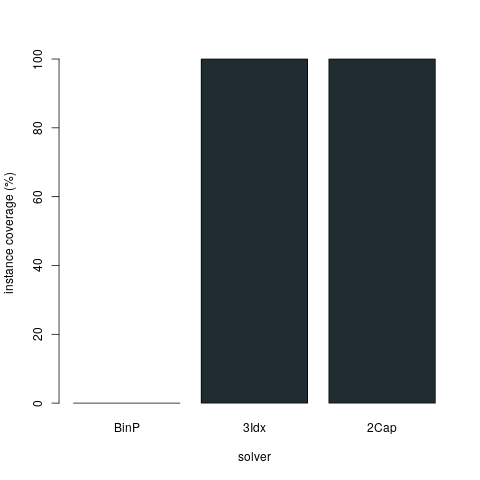
\includegraphics[width=1.1\textwidth]{img/solver_instance_coverage_b=2_m_60s.png}
\caption{\textsc{Zeitlimit} $1min$}
\label{fig:instance_cov_b=2_m_b}
\end{subfigure}
\hfill
\begin{subfigure}[b]{0.3\textwidth}
\centering
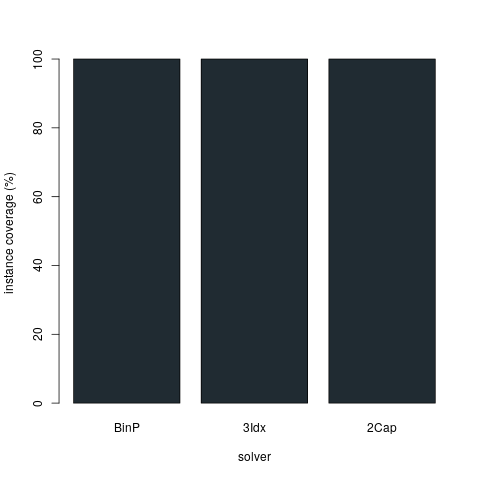
\includegraphics[width=1.1\textwidth]{img/solver_instance_coverage_b=2_m_120s.png}
\caption{\textsc{Zeitlimit} $2min$}
\label{fig:instance_cov_b=2_m_c}
\end{subfigure}
\caption{\textsc{Instance-Coverage der $b=2$ Solver (m)}.}
\label{fig:instance_cov_b=2}
\end{figure}

In Abb. \ref{fig:res_plots_b=2_m} sind die Laufzeiten und ermittelten Zielfunktionswerte der Solver bei einem Zeitlimit von zwei Minuten dargestellt. Die 3-Index-Formulierung terminiert, wie Abb. \ref{fig:b=2_m_runtimes} zu entnehmen ist, bei jeder Instanz vor dem Zeitlimit, was bedeutet, dass diese sämtliche Instanzen optimal löst. Die Bin-Packing-Formulierung gelangt dagegen in keinem Fall zur Optimallösung (vgl. Abb. \ref{fig:b=2_m_costs}).
In Abb. \ref{fig:b=2_m_runtimes} ist zu erkennen, dass die Bin-Packing-Formulierung deutlich längere Laufzeiten als die 3-Index-Formulierung und die Heurisktik besitzt, wobei die Heuristik beide MIP-Formulierungen deutlich unterbietet.
Der Laufzeitunterschied zwischen der Heuristik und der 3-Index-Formulierung ist deutlich größer als jener zwischen den beiden MIP-Formulierungen. Zwischen der Heuristik, welche durchschnittlich $0.39s$ benötigt und der 3-Index-Formulierung, die durchschnittlich $37.49s$ benötigt (vgl. Abb. \ref{fig:res_b=2_m_c}), besteht ein Faktor von $96.1$, während zwischen den beiden MIP-Formulierungen nur ein Faktor von $3.4$ besteht. Die Darstellung der absoluten Laufzeitdifferenzen ist in diesem Fall also etwas irreführend, da die Heuristik deutlich schneller ist als beide MIP-Formulierungen. Trotzdem ist die 3-Index-Formulierung aus praktischer Perspektive klar der Bin-Packing-Formulierung vorzuziehen, dieser Sachverhalt ist in Abb. \ref{fig:b=2_m_runtimes} gut erkennbar.
Die Bin-Packing-Formulierung gelangt nicht nur in keinem Fall zu einer Optimallösung, sondern weicht zusätzlich,
wie man Abb. \ref{fig:b=2_m_costs} entnehmen kann, bei jeder Instanz in erheblichem Maße vom optimalen Zielfunktionswert ab, weshalb sie in dieser Kategorie in keinem Fall konkurrenzfähig ist. Demgegenüber kommt die Heuristik den optimalen Zielfunktionswerten mit geringen Abweichungen in jedem Fall sehr nahe.
Die Stacking-Constraints haben, wie man an den ebenfalls in Abb. \ref{fig:b=2_m_costs} dargestellten unteren Schranken erkennen kann, in dieser Kategorie bei jeder Instanz einen Einfluss auf den optimalen Zielfunktionswert,
wenngleich dieser erneut i.d.R. sehr gering ausfällt.
Die Darstellung der Kosten in Abb. \ref{fig:b=2_m_costs} wurde erneut in einer Weise skaliert, welche
es ermöglicht, sämtliche Einträge zu erkennen. Die tatsächlichen Abstände sind den Beschriftungen der $x$-Achse zu entnehmen.

\begin{figure}[H]
\centering
\begin{subfigure}[b]{0.47\textwidth}
\centering
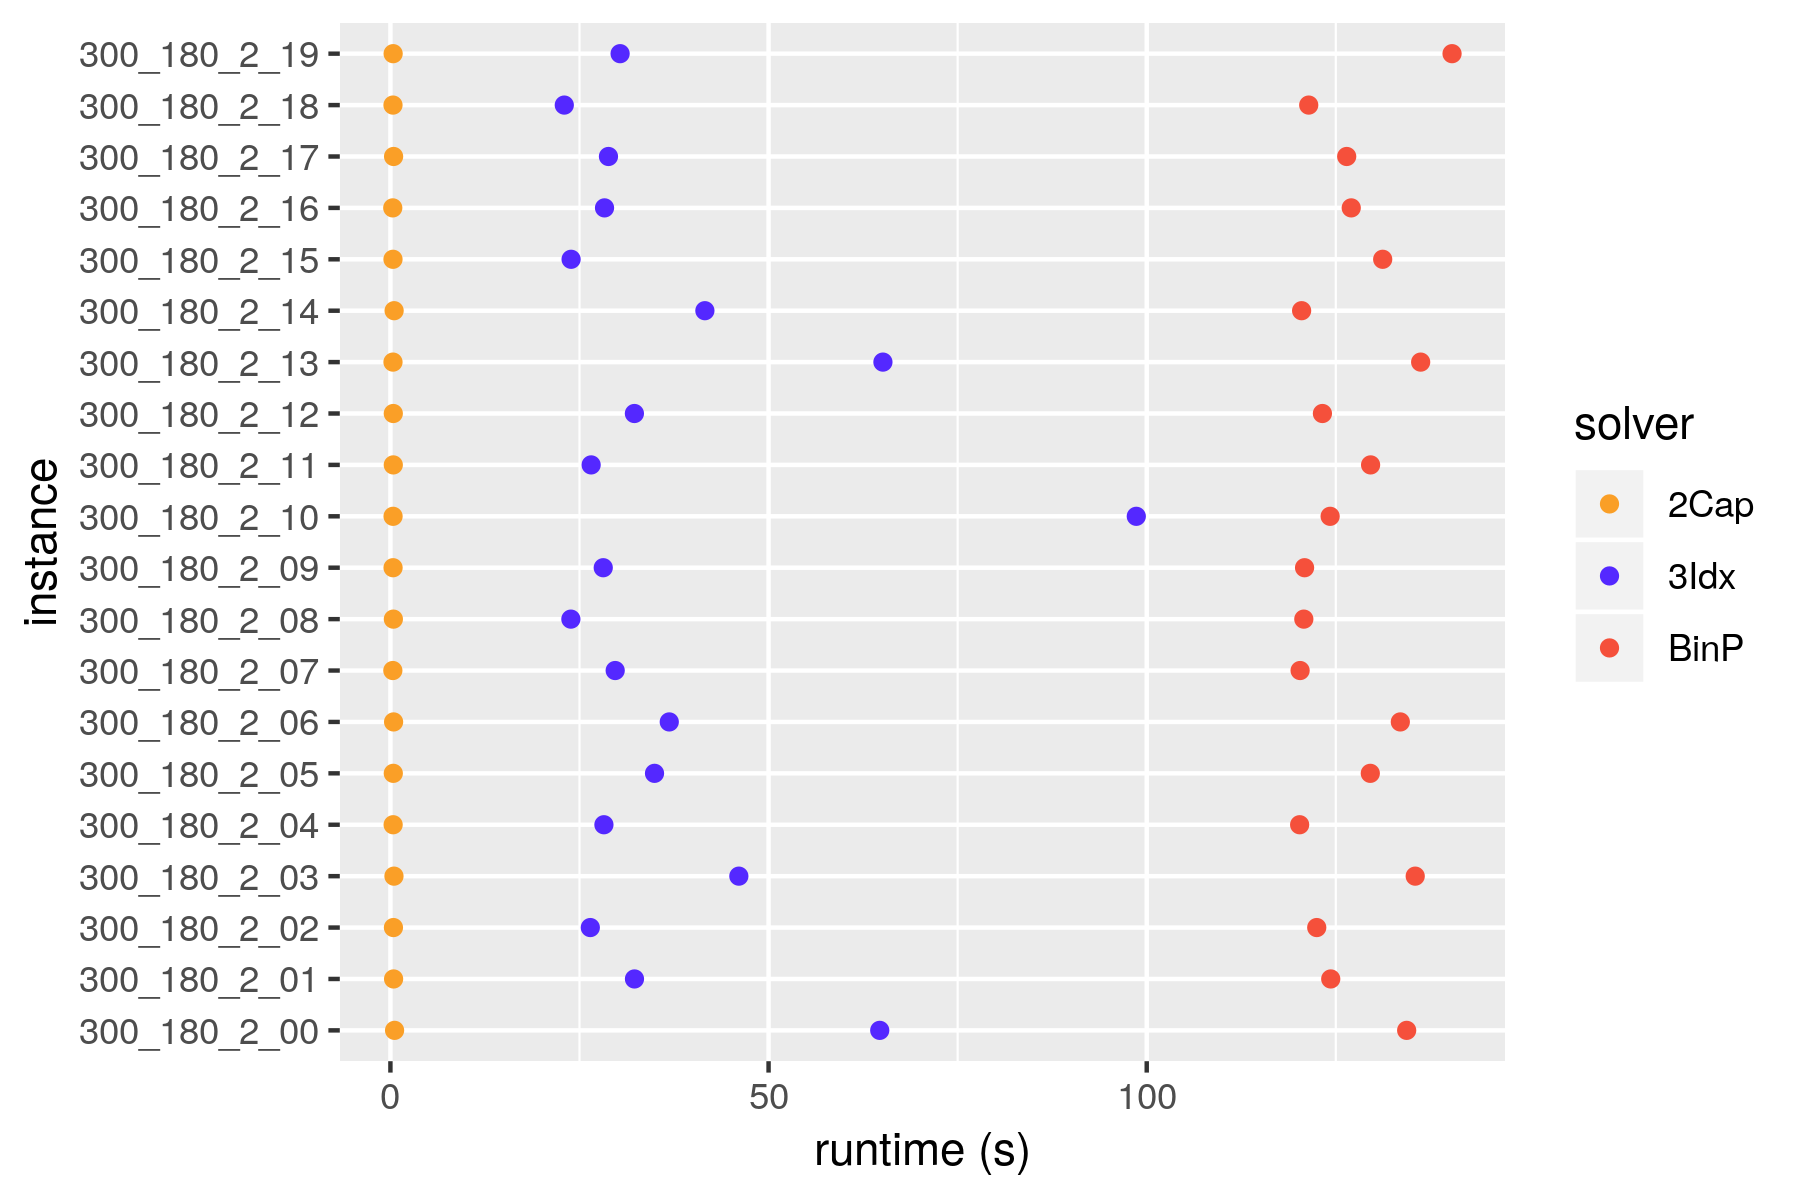
\includegraphics[width=1.1\textwidth]{img/solver_instance_time_b=2_m_120s.png}
\caption{\textsc{Laufzeiten}}
\label{fig:b=2_m_runtimes}
\end{subfigure}
\hfill
\begin{subfigure}[b]{0.47\textwidth}
\centering
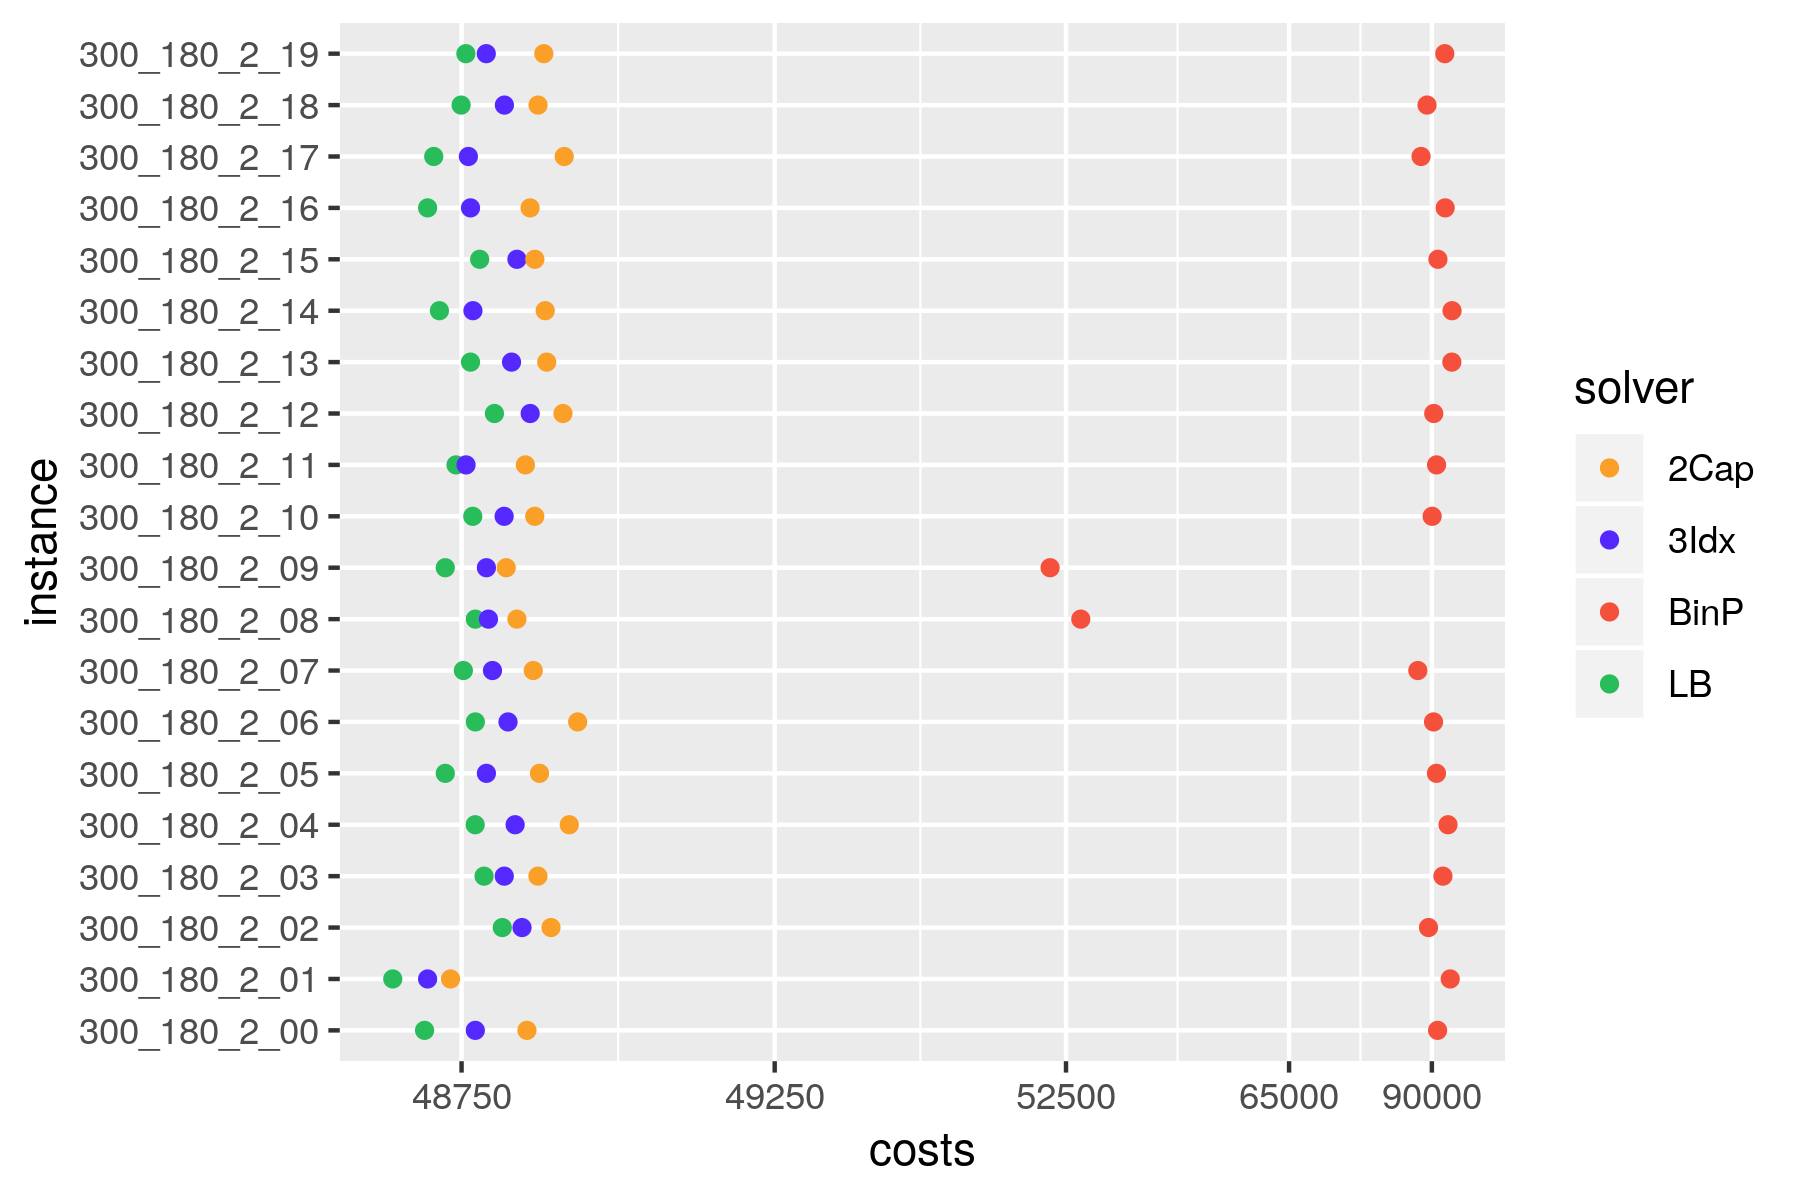
\includegraphics[width=1.1\textwidth]{img/solver_instance_cost_b=2_m_120s.png}
\caption{\textsc{Kosten}}
\label{fig:b=2_m_costs}
\end{subfigure}
\caption{\textsc{Ergebnisse bei $2min$ Zeitlimit}.}
\label{fig:res_plots_b=2_m}
\end{figure}

In den Tabellen in Abb. \ref{fig:res_b=2_m} können die exakten Ergebnisse der MIP-Formulierungen nachvollzogen werden.
Wie bereits erwähnt, hat die Bin-Packing-Formulierung bei einem Zeitlimit von $30s$ keine Instanz zulässig gelöst, die 3-Index-Formulierung löst dort sämtliche Instanzen zulässig, allerdings nur $65 \%$ optimal (vgl. Abb. \ref{fig:res_b=2_m_a}). Dafür benötigt diese durchschnittlich $28.47s$ und weicht um durchschnittlich $9.99 \%$ vom Optimum ab.
Die Heuristik löst sämtliche Instanzen zulässig, benötigt dafür durchschnittlich $0.4s$ und weicht um durchschnittlich $0.06 \%$ vom Optimum ab. Damit ist die Heuristik bei einem Zeitlimit von $30s$ im Durchschnitt sogar um mehrere Größenordnungen näher am Optimum als die 3-Index-Formulierung. Wie man Abb. \ref{fig:res_b=2_m_b} entnehmen kann, löst die 3-Index-Formulierung bei einem Zeitlimit von einer Minute $85 \%$ der Instanzen optimal und benötigt dafür durchschnittliche $35.2s$. Da diese dabei um durchschnittlich $1.86 \%$ vom Optimum abweicht, liefert die Heuristik weiterhin neben der Laufzeit auch bei den Zielfunktionswerten deutlich bessere Ergebnisse. Die Bin-Packing-Formulierung löst auch bei diesem Zeitlimit keine Instanz zulässig. Beim letzten betrachteten Zeitlimit von zwei Minuten löst die 3-Index-Formulierung schließlich mit einer Laufzeit von durchschnittlich $37.49s$ sämtliche Instanzen optimal, während die Bin-Packing-Formulierung bei diesem Zeitlimit zwar sämtliche Instanzen zulässig löst, jedoch bei keiner Instanz zum optimalen Zielfunktionswert gelangt und aufgrund der erheblichen Abweichungen, welche bereits in Abb. \ref{fig:b=2_m_costs} deutlich wurden, in keinem Fall konkurrenzfähig ist (vgl. Abb. \ref{fig:res_b=2_m_c}).

\vfill
\pagebreak

\begin{figure}[H]
\centering
% \end{figure}
% \begin{figure}[H]
% $\quad\quad\quad\quad$
\begin{subfigure}[b]{0.3\textwidth}
\centering
\resizebox{\textwidth}{!}{
\begin{tabular}{ | c | c | c |}
    \hline
     & \textbf{BinP} & \textbf{3Idx} \\ \hline
    \textbf{Optimal ($\boldsymbol{\%}$)} & $ \textcolor{red}{0}$ & $ \textcolor{mygreen}{65}$ \\ \hline
    \textbf{\O \thinspace Laufzeit ($\boldsymbol{s}$)} & $\textcolor{red}{-}$ & $\textcolor{mygreen}{28.47}$ \\ \hline
    \textbf{\O \thinspace Abweichung ($\boldsymbol{\%}$)} & $\textcolor{red}{-}$ &$\textcolor{mygreen}{9.99}$ \\ \hline
\end{tabular}}
\caption{\textsc{Zeitlimit} $30s$}
\label{fig:res_b=2_m_a}
\end{subfigure}
\begin{subfigure}[b]{0.3\textwidth}
\centering
\resizebox{\textwidth}{!}{
\begin{tabular}{ | c | c | c |}
    \hline
     & \textbf{BinP} & \textbf{3Idx} \\ \hline
    \textbf{Optimal ($\boldsymbol{\%}$)} & $ \textcolor{red}{0}$ & $ \textcolor{mygreen}{85}$ \\ \hline
    \textbf{\O \thinspace Laufzeit ($\boldsymbol{s}$)} & $\textcolor{red}{-}$ & $\textcolor{mygreen}{35.2}$ \\ \hline
    \textbf{\O \thinspace Abweichung ($\boldsymbol{\%}$)} & $\textcolor{red}{-}$ & $\textcolor{mygreen}{1.86}$ \\ \hline
\end{tabular}}
\caption{\textsc{Zeitlimit} $1min$}
\label{fig:res_b=2_m_b}
\end{subfigure}
% \end{figure}
% \begin{figure}[H]
\begin{subfigure}[b]{0.3\textwidth}
\centering
\resizebox{\textwidth}{!}{
\begin{tabular}{ | c | c | c |}
    \hline
     & \textbf{BinP} & \textbf{3Idx} \\ \hline
    \textbf{Optimal ($\boldsymbol{\%}$)} & $\textcolor{red}{0}$ & $\textcolor{mygreen}{100}$ \\ \hline
    \textbf{\O \thinspace Laufzeit ($\boldsymbol{s}$)} & $\textcolor{red}{127.12}$ & $\textcolor{mygreen}{37.49}$ \\ \hline
    \textbf{\O \thinspace Abweichung ($\boldsymbol{\%}$)} & $\textcolor{red}{79.94}$ & $\textcolor{mygreen}{0.0}$ \\ \hline
\end{tabular}}
\caption{\textsc{Zeitlimit} $2min$}
\label{fig:res_b=2_m_c}
\end{subfigure}
\caption{\textsc{MIP-Ergebnisse}.}
\label{fig:res_b=2_m}
\end{figure}

Zusammenfassend ist die 3-Index-Formulierung in der Kategorie der mittelgroßen Instanzen der Bin-Packing-Formulierung vorzuziehen, da diese bei allen betrachteten Zeitlimits die besseren Ergebnisse erzielt.
Der Laufzeitunterschied zwischen der Heuristik und der zu bevorzugenden MIP-Formulierung ist so erheblich,
dass die sehr geringe Abweichung vom Optimum in der Praxis in Kauf genommen werden sollte.
In dieser Kategorie stellt sich die Heuristik demzufolge als sehr gute Alternative heraus.\newline

\textbf{Große Instanzen (l)}

Zuletzt werden die Solver für in Kapitel \ref{sec:test_data} als groß bezeichnete Instanzen, bei denen es darum geht,
$500$ eintreffende Items in die Storage-Area zu verladen, verglichen. In dieser Kategorie wurden noch einmal größere Zeitlimits von $5$, $10$ und $20$ Minuten betrachtet.

In Abb. \ref{fig:instance_cov_b=2_l} ist die Instance-Coverage der Solver für die jeweiligen Zeitlimits dargestellt.
Bei einem Zeitlimit von $5$ Minuten findet die Bin-Packing-Formulierung für keine Instanz eine zulässige Lösung,
während die 3-Index-Formulierung dort bereits sämtliche Instanzen zulässig löst (vgl. Abb \ref{fig:instance_cov_b=2_l_a}). Beim nächstgrößeren Zeitlimit von $10$ Minuten löst die Bin-Packing-Formulierung weiterhin lediglich $10 \%$ der Instanzen zulässig (vgl. Abb. \ref{fig:instance_cov_b=2_l_b}). Erst beim letzten betrachteten Zeitlimit von $20$ Minuten besitzt schließlich auch die Bin-Packing-Formulierung eine vollständige Instance-Coverage (vgl. Abb. \ref{fig:instance_cov_b=2_l_c}). Es ist somit bereits klar, dass in dieser Kategorie bei einer zur Verfügung stehenden Zeit von weniger als $10$ Minuten stets die 3-Index-Formulierung der Bin-Packing-Formulierung vorgezogen werden sollte. Für die Heuristik sind die Zeitlimits erneut irrelevant, da diese mit einer durchschnittlichen Laufzeit von $1.7s$ pro Instanz sämtliche Instanzen zulässig löst.

\begin{figure}[H]
\centering

\begin{subfigure}[b]{0.3\textwidth}
\centering
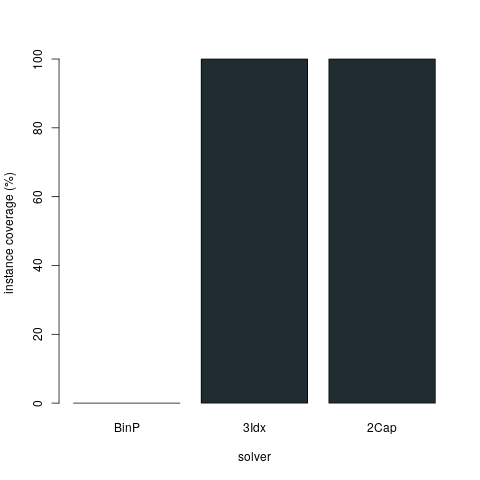
\includegraphics[width=1.1\textwidth]{img/solver_instance_coverage_b=2_l_300s.png}
\caption{\textsc{Zeitlimit} $5min$}
\label{fig:instance_cov_b=2_l_a}
\end{subfigure}
\hfill
\begin{subfigure}[b]{0.3\textwidth}
\centering
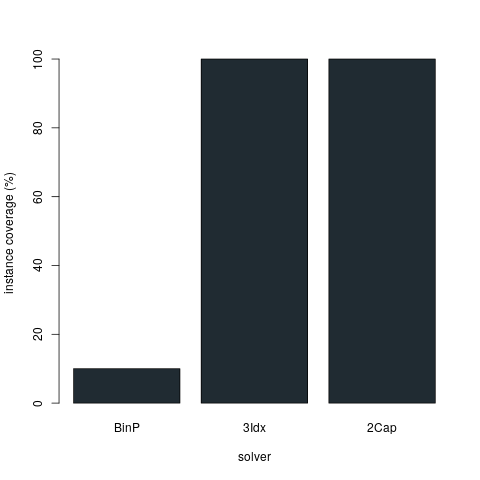
\includegraphics[width=1.1\textwidth]{img/solver_instance_coverage_b=2_l_600s.png}
\caption{\textsc{Zeitlimit} $10min$}
\label{fig:instance_cov_b=2_l_b}
\end{subfigure}
\hfill
\begin{subfigure}[b]{0.3\textwidth}
\centering
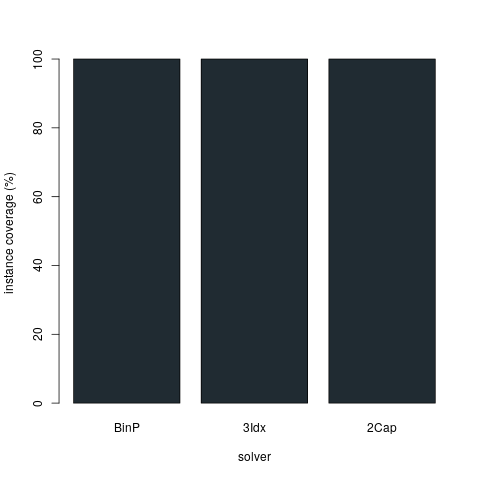
\includegraphics[width=1.1\textwidth]{img/solver_instance_coverage_b=2_l_1200s.png}
\caption{\textsc{Zeitlimit} $20min$}
\label{fig:instance_cov_b=2_l_c}
\end{subfigure}

\caption{\textsc{Instance-Coverage der $b=2$ Solver (l)}.}
\label{fig:instance_cov_b=2_l}
\end{figure}

\vfill
\pagebreak

In Abb. \ref{fig:res_plots_b=2_l}, in welcher die Laufzeiten und ermittelten Zielfunktionswerte der Solver bei
einem Zeitlimit von $20$ Minuten dargestellt sind, bestätigt sich die Tendenz aus der Darstellung der Instance-Coverage.
Die Heuristik ist deutlich schneller als die 3-Index-Formulierung (vgl. Abb. \ref{fig:b=2_l_runtimes}) und weicht dabei nur unwesentlich von den optimalen Zielfunktionswerten ab. Mit Instanz $03$ wird in dieser Kategorie sogar eine Instanz optimal von der Heuristik gelöst (vgl. Abb. \ref{fig:b=2_l_costs}). Außerdem ist die 3-Index-Formulierung, wie zu erwarten, in der Regel schneller als die Bin-Packing-Formulierung. Bemerkenswert ist allerdings, dass die Bin-Packing-Formulierung im Gegensatz zur 3-Index-Formulierung stets vor dem Zeitlimit terminiert und somit sämtliche Instanzen optimal löst, wenn auch mitunter nur sehr knapp.
Die 3-Index-Formulierung wird dagegen mit den Instanzen $04, 09, 11, 16$ und $19$ in fünf Fällen durch das Zeitlimit gestoppt, in welchen diese entsprechend jeweils längere Laufzeiten als die Bin-Packing-Formulierung besitzt.
Wie man Abb. \ref{fig:b=2_l_costs} entnehmen kann, äußert sich dies in deutlich abweichenden Zielfunktionswerten bei diesen Instanzen, welche sogar von der Heuristik in jedem Fall sehr deutlich unterboten werden.
Nach den Ergebnissen der Instance-Coverage ist es durchaus überraschend, dass die Bin-Packing-Formulierung letztlich sämtliche Instanzen optimal löst, während die 3-Index-Formulierung bei fünf Instanzen deutlich vom Optimum abweicht.
Die Heuristik kommt den optimalen Zielfunktionswerten auch in dieser Kategorie mit geringen Abweichungen sehr nahe
und die Einträge der unteren Schranken zeigen, dass die Stacking-Constraints bei jeder
betrachteten Instanz einen deutlichen Einfluss auf die optimalen Zielfunktionswerte haben.
Die Darstellung der Kosten wurde erneut in einer Weise skaliert, welche eine Betrachtung sämtlicher Einträge ermöglicht.

\begin{figure}[H]
\centering
\begin{subfigure}[b]{0.4\textwidth}
\centering
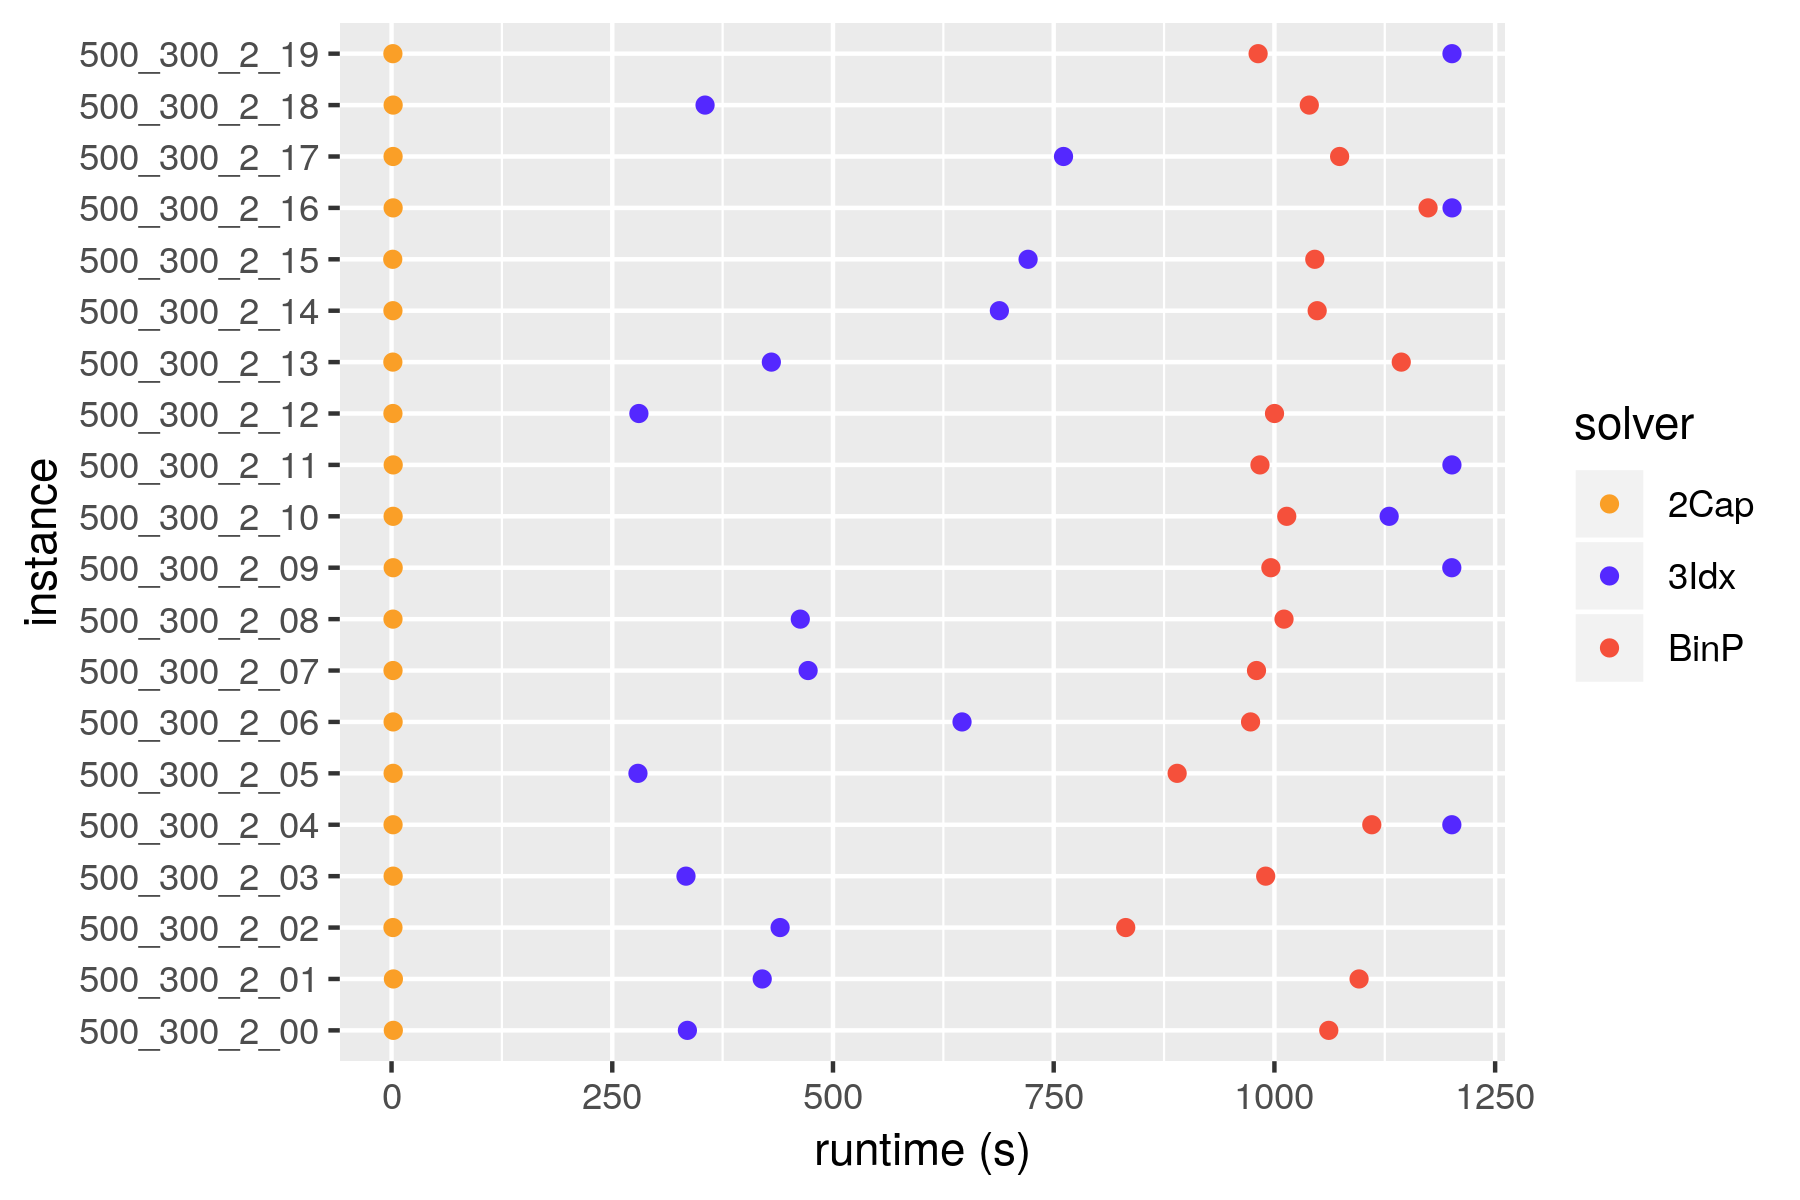
\includegraphics[width=1.3\textwidth]{img/solver_instance_time_b=2_l_1200s.png}
\caption{\textsc{Laufzeiten}}
\label{fig:b=2_l_runtimes}
\end{subfigure}
\hfill
\begin{subfigure}[b]{0.4\textwidth}
\centering
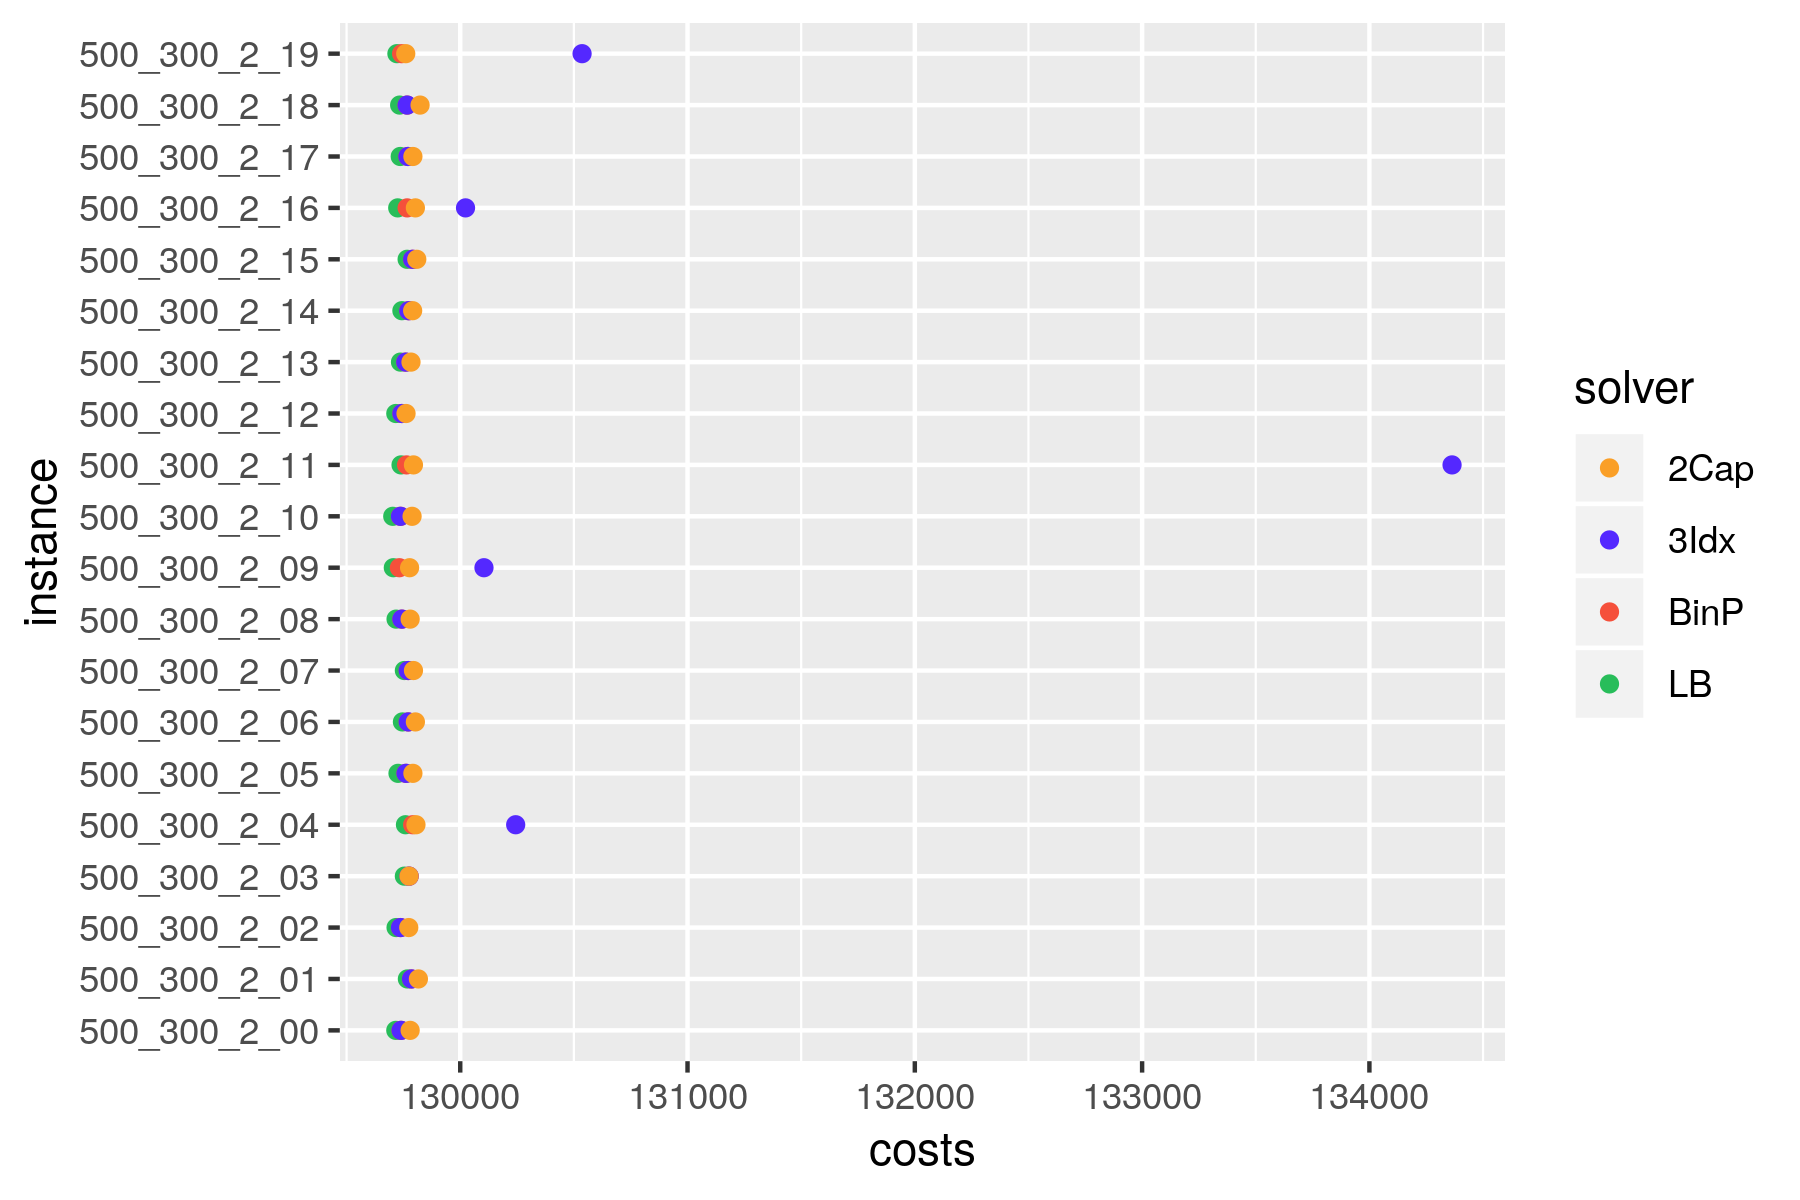
\includegraphics[width=1.3\textwidth]{img/solver_instance_cost_b=2_l_1200s.png}
\caption{\textsc{Kosten}}
\label{fig:b=2_l_costs}
\end{subfigure}
\caption{\textsc{Ergebnisse bei $20min$ Zeitlimit}.}
\label{fig:res_plots_b=2_l}
\end{figure}

In Abb. \ref{fig:res_b=2_l} sind die exakten Ergebnisse der MIP-Formulierungen aufgeführt, denen man
entnehmen kann, dass die Bin-Packing-Formulierung mit einer durchschnittlichen Laufzeit von ca. $17$ Minuten sämtliche Instanzen optimal löst (vgl. Abb. \ref{fig:res_b=2_l_c}). Wie bereits anhand der Instance-Coverage deutlich wurde,
kommt die 3-Index-Formulierung bei Zeitlimits von unter $20$ Minuten zu deutlich besseren Ergebnissen als die Bin-Packing-Formulierung (vgl. Abb. \ref{fig:res_b=2_l_a}, \ref{fig:res_b=2_l_b}). Allerdings löst diese bei keinem der betrachteten Zeitlimits sämtliche Instanzen optimal, was der Bin-Packing-Formulierung beim Zeitlimit von $20$ Minuten gelingt, wenn auch bei einer im Durschschnitt deutlich längeren Laufzeit (vgl. Abb. \ref{fig:res_b=2_l_c}). Da die Ergebnisse nahelegen, dass die 3-Index-Formulierung
bei einer geringfügigen Erhöhung des Zeitlimits ebenfalls sämtliche Instanzen optimal löst, wurde ein weiteres Experiment mit einem Zeitlimit von $30$ Minuten pro Instanz durchgeführt. Auch in diesem konnte die 3-Index-Formulierung mit $95 \%$ noch nicht sämtliche Instanzen optimal lösen. In diesem Fall ist das Ergebnis daher nicht eindeutig. Bei Zeitlimits von unter $20$ Minuten sollte die 3-Index-Formulierung bevorzugt werden. Stehen $20$ Minuten und mehr pro Instanz zur Verfügung, so sollte die Bin-Packing-Formulierung bevorzugt werden. Die 3-Index-Formulierung löst erst bei Zeitlimits von mehr als $30$ Minuten pro Instanz sämtliche Instanzen optimal, weshalb der Laufzeitvorteil gegenüber der Bin-Packing-Formulierung aufgrund der Instanzen, welche deutlich längere Laufzeiten benötigen, nicht mehr erheblich sein dürfte. Dementsprechend sollte ab einem Zeitlimit von $20$ Minuten durchaus die Bin-Packing-Formulierung bevorzugt werden.

\begin{figure}[H]
\begin{subfigure}[b]{0.3\textwidth}
\centering
\resizebox{\textwidth}{!}{
\begin{tabular}{ | c | c | c |}
    \hline
     & \textbf{BinP} & \textbf{3Idx} \\ \hline
    \textbf{Optimal ($\boldsymbol{\%}$)} & $\textcolor{red}{0}$ & $ \textcolor{mygreen}{15}$ \\ \hline
    \textbf{\O \thinspace Laufzeit ($\boldsymbol{s}$)} & \textcolor{red}{$-$} & $\textcolor{mygreen}{299.25}$ \\ \hline
    \textbf{\O \thinspace Abweichung ($\boldsymbol{\%}$)} & \textcolor{red}{$-$} & $\textcolor{mygreen}{33.31}$ \\ \hline
\end{tabular}}
\caption{\textsc{Zeitlimit} $5min$}
\label{fig:res_b=2_l_a}
\end{subfigure}
\begin{subfigure}[b]{0.3\textwidth}
\centering
\resizebox{\textwidth}{!}{
\begin{tabular}{ | c | c | c |}
    \hline
     & \textbf{BinP} & \textbf{3Idx} \\ \hline
    \textbf{Optimal ($\boldsymbol{\%}$)} & $ \textcolor{red}{0}$ & $ \textcolor{mygreen}{55}$ \\ \hline
    \textbf{\O \thinspace Laufzeit ($\boldsymbol{s}$)} & \textcolor{red}{$605.07$} & $ \textcolor{mygreen}{490.64}$ \\ \hline
    \textbf{\O \thinspace Abweichung ($\boldsymbol{\%}$)} & \textcolor{red}{$61.55$} & $\textcolor{mygreen}{3.83}$ \\ \hline
\end{tabular}}
\caption{\textsc{Zeitlimit} $10min$}
\label{fig:res_b=2_l_b}
\end{subfigure}
% $\quad\quad\quad\quad$
\begin{subfigure}[b]{0.3\textwidth}
\centering
\resizebox{\textwidth}{!}{
\begin{tabular}{ | c | c | c |}
    \hline
     & \textbf{BinP} & \textbf{3Idx} \\ \hline
    \textbf{Optimal ($\boldsymbol{\%}$)} & $ \textcolor{mygreen}{100}$ & $ \textcolor{red}{75}$ \\ \hline
    \textbf{\O \thinspace Laufzeit ($\boldsymbol{s}$)} & \textcolor{red}{$1022.17$} & $\textcolor{mygreen}{687.99}$ \\ \hline
    \textbf{\O \thinspace Abweichung ($\boldsymbol{\%}$)} & \textcolor{mygreen}{$0.0$} & $\textcolor{red}{0.25}$ \\ \hline
\end{tabular}}
\caption{\textsc{Zeitlimit} $20min$}
\label{fig:res_b=2_l_c}
\end{subfigure}

\caption{\textsc{MIP-Ergebnisse}}
\label{fig:res_b=2_l}
\end{figure}

Die Heuristik löst die Instanzen allerdings nach nur durchschnittlich $1.7s$ pro Instanz und weicht auch nur um im Durchschnitt $0.02 \%$ vom Optimalwert ab. Dieser, verglichen mit der Kategorie der mittelgroßen Instanzen, noch gravierendere Laufzeitunterschied und die zu vernachlässigende Abweichung vom Optimum sorgen dafür, dass die Heuristik in der Praxis erneut klar bevorzugt werden sollte. Selbst in Bezug auf die Qualität der Zielfunktionswerte können die MIP-Formulierungen erst ab dem betrachteten Zeitlimit von $20$ Minuten mit denen der Heuristik konkurrieren, wobei die 3-Index-Formulierung, wie man Abb. \ref{fig:res_b=2_l_c} entnehmen kann, selbst dort mit einer durchschnittlichen Abweichung von $0.25 \%$ vom Optimum noch erheblich schlechtere Zielfunktionswerte liefert als die Heuristik.

\textbf{Fazit}

Insgesamt ist festzuhalten, dass bei Stacking-Problemen mit Stacks der Kapazität $b = 2$ in der Kategorie der kleinen Instanzen aufgrund der geringen Laufzeit der MIP-Formulierungen kein wirklicher Bedarf für eine Laufzeitverbesserung besteht. Anders in den Kategorien der mittelgroßen und großen Instanzen, bei welchen die Heuristik bei sehr geringen Abweichungen von den Optimalwerten zu einer derart großen Laufzeitersparnis führt, dass diese eine in der Praxis relevante Alternative darstellt.

In Bezug auf den Vergleich der MIP-Formulierungen untereinander gilt, dass die 3-Index-Formulierung in den Kategorien
der kleinen und mittelgroßen Instanzen zu bevorzugen ist, während die Bin-Packing-Formulierung ab einem Zeitlimit
von $20$ Minuten bei den großen Instanzen zu besseren Ergebnissen führt.

\subsection{Konstruktive Heuristik ($b = 3$)}
\label{sec:three_cap_heuristic}

Die konstruktive Heuristik zur Lösung von Stacking-Problemen mit Stacks der Kapazität $b = 3$ funktioniert
an einigen Stellen analog zur Heuristik aus Abschnitt \ref{sec:two_cap_heuristic} für eine Stack-Kapazität von $b = 2$.
Um den zusätzlichen Möglichkeiten und Anforderungen der erhöhten Stack-Kapazität gerecht zu werden, werden überdies
erweiternde Ansätze präsentiert.

\vfill
\pagebreak

Zunächst geht es, wie auch in der Heuristik für $b = 2$, darum, kompatible Item-Paare zu bilden.
Dazu wird, analog zur Heuristik aus Abschnitt \ref{sec:two_cap_heuristic}, ein Stacking-Graph $G = (V, E)$ generiert.
Berechnet man ein \textsc{MCM} $M \subseteq E$ in $G$ und interpretiert dessen Kanten $\{i, j\} \in M$ als Paare kompatibler Items $i, j \in I$, so erhält man eine größtmögliche Anzahl von Item-Paaren, welche in mindestens einer Richtung stapelbar sind.
In der Regel ist anschließend basierend auf den Stacking-Constraints die Mehrheit oder sogar die Gesamtheit der Items einer Instanz Teil eines Paares, weshalb sich die weitere Berechnung eines \textsc{MCM} zwischen Item-Paaren und Unmatched-Items,
um erste Tripel zu bilden, welche in einer früheren Version der Heuristik an dieser Stelle stattfand, als nicht zielführend
erwies.

Da die Stacks nun nicht nur Paare, sondern Tripel von Items beinhalten können, geht es im Folgenden darum,
ebensolche Tripel von kompatiblen Items zu generieren. Dazu werden die zuvor gebildeten Item-Paare zu Item-Tripeln zusammengeführt.
Zunächst muss allerdings entschieden werden, welche dieser Paare sinnvollerweise wieder separiert werden sollten,
um beide Items einem jeweils anderen Paar zuzuweisen und zwei Tripel zu bilden. Dies geschieht mithilfe eines Rating-Systems, welches die Item-Paare mit dem Ziel bewertet, jene Paare zu ermitteln, die im Hinblick auf ein günstiges Ergebnis
und möglichst vollständig gefüllte Stacks getrennt werden sollten.

\textbf{Rating-System}

Initial wird jede Kante $\{i, j\} \in M$, also jedes Item-Paar, mit dem Basis-Rating $0$ bewertet.
Anschließend wird für jedes dieser Paare die Kompatibilität seiner Items $i, j \in I$ zu anderen Paaren aus $M \textbackslash \{i, j\}$ ermittelt.
Dementsprechend wird für jedes Item, welches Teil eines Paares ist, die Anzahl der verbleibenden Paare bestimmt, zu denen es kompatibel ist, denen es also zugewiesen werden kann, um ein Tripel zu bilden. Diese Kompatibilität bezieht sich auf die Stacking-Constraints.
Eine Menge von Items ist zueinander kompatibel, wenn diese basierend auf den Stacking-Constraints in mindestens einer
Reihenfolge gestapelt werden kann.

Geht es beispielsweise darum, zu überprüfen, ob ein Item $i \in I$ einem Paar $(s, t)$, welches aus einer Kante $\{s, t\} \in M$ resultiert,
zugewiesen werden kann, so ergeben sich die in Abb. \ref{fig:triple_permutations} dargestellten $3!$ möglichen Permutationen eines Tripels. Stellt sich eine dieser Permutationen als konform mit den Stacking-Constraints heraus, so kann das Item $i$ zusammen mit dem Paar $(s, t)$ ein zulässiges Tripel bilden.
\begin{figure}[H]
\[
\begin{bmatrix}
  \boldsymbol{i} & s & s & \boldsymbol{i} & t & t \\
  s & \boldsymbol{i} & t & t & \boldsymbol{i} & s \\
  t & t & \boldsymbol{i} & s & s & \boldsymbol{i}
\end{bmatrix}
\]
\caption{\textsc{Item-Tripel Permutationen.}}
\label{fig:triple_permutations}
\end{figure}
Sind die Items $s, t \in I$, welche das betrachtete Paar bilden, in beide Richtungen stapelbar, also
$s_{st} + s_{ts} = 2$, so sind sämtliche Permutationen zu überprüfen.
Aufgrund der Transitivität der Stacking-Constraints ist das Item $i$ in diesem Fall allerdings bereits dann kompatibel zum Paar $(s, t)$,
wenn $s_{is} + s_{it} + s_{si} + s_{ti} \geq 1$ gilt.
Darf Item $s$ auf Item $t$ gestapelt werden, jedoch nicht andersherum, also $s_{st} = 1$ und $s_{ts} = 0$,
so müssen die ersten drei Permutationen überprüft werden. Item $i$ ist dann kompatibel zum Paar $(s, t)$,
wenn $s_{is} + s_{ti} \geq 1$ oder $s_{si} + s_{it} = 2$ gilt.
Gilt umgekehrt, dass lediglich Item $t$ auf Item $s$ gestapelt werden darf, also $s_{st} = 0$ und $s_{ts} = 1$, so
müssen die letzten drei Permutationen überprüft werden und Item $i$ ist kompatibel zum Paar $(s, t)$,
wenn $s_{it} + s_{si} \geq 1$ oder $s_{ti} + s_{is} = 2$ gilt.\newline
Auf diese Weise wird die Kompatibilität sämtlicher Items, welche Teil eines Paares sind, zu den verbleibenden Paaren bestimmt.
Ausschlaggebend ist dabei jeweils die Anzahl der kompatiblen Paare des weniger kompatiblen Items eines Paares,
da stets beide Items erneut zugewiesen werden müssen. Diese wird im Folgenden als \textquote{Worst-Compatibility}
$w_{ij}$ des Item-Paares $(i, j)$ bezeichnet.

Des Weiteren werden für jedes Item-Paar $(i, j)$ die durchschnittlichen Kosten einer gemeinsamen Stack-Zuweisung berechnet.
Zu diesem Zweck werden zunächst die durchschnittlichen Kosten $a$ einer zulässigen Zuweisung eines Items zu einem Stack berechnet,
also der Durchschnitt aller Einträge $c_{iq}$ für Items $i \in I$ und Stacks $q \in Q$ in der Transportkostenmatrix $C$, für
die $t_{iq} = 1$ gilt. Dabei entspricht $c_{(i, j)q}$ jeweils den Kosten der gemeinsamen Zuweisung der Items $i$ und $j$ zu Stack $q$,
welche wie folgt definiert sind:
\[
    c_{(i, j)q} \quad := \quad
\begin{cases}
    c_{iq} + c_{jq}, & \text{wenn $t_{iq} = 1$ und $t_{jq} = 1$}\\
    za, & \text{sonst}
\end{cases}
\]
D.h. die Kosten der Zuweisung entsprechen nur dann der Summe der beiden Einzelzuweisungen, wenn beide Items des Paares basierend
auf den Placement-Constraints kompatibel zum Stack sind. Ist dies nicht der Fall, so wird die Inkompatibilität durch
einen Kostenwert von $za$ mit $z \in \mathbb{R}$, also dem $z$-fachen der Kosten einer durchschnittlichen Item-Stack-Zuweisung, bestraft. Der durchschnittliche Kostenwert $avgC_{ij}$, für das Item-Paar $(i, j)$, ergibt sich folgendermaßen:
\[ avgC_{ij} = \frac{\sum_{q \in Q} c_{(i, j)q}}{|Q|}  \]

Anschließend wird über sämtliche Paare, die sich aus den Kanten $\{i, j\} \in M$ ergeben, hinweg eine durchschnittliche \textquote{Worst-Compatibility} $w$, also eine durchschnittliche Kompatibilität des jeweils weniger kompatiblen Items, sowie ein durchschnittlicher Kostenwert $avgC$ für Stackzuweisungen berechnet. Wenn ein Paar $(i, j)$ nun sowohl eine über dem Durchschnitt liegende \textquote{Worst-Compatibility} $w_{ij} > w$, als auch einen über dem Durchschnitt liegenden durchschnittlichen Kostenwert $avgC_{ij} > avgC$ besitzt, scheint es gut geeignet für eine Separation,
denn es ist überdurchschnittlich flexibel für eine erneute Zuweisung und seine gegenwärtige Zuweisung ist ohnehin überdurchschnittlich teuer.
Dabei ist selbstverständlich nicht garantiert, dass für diese Items nach der Trennung eine günstigere Zuweisung existiert.

Wenn die Summe der prozentualen Abweichungen $d_{ij}$ beider Werte des Paares $(i, j)$ vom Durchschnitt einen gewissen Schwellenwert,
welcher im Folgenden als \textquote{Deviation-Threshold} $d_t$ bezeichnet wird,
überschreitet, entspricht das Rating $r_{ij}$ des Paares ebendieser Summe.
Die Summe der prozentualen Abweichungen $d_{ij}$ ist wie folgt definiert:
\[ d_{ij} = \frac{|avgC - avgC_{ij}|}{avgC \cdot 100} + \frac{|w - w_{ij}|}{w \cdot 100}\]
Das Rating $r_{ij}$ des Paares $(i, j)$ ergibt sich dementsprechend folgendermaßen:
\[
    r_{ij} \quad := \quad
\begin{cases}
    d_{ij}, & \text{wenn $d_{ij} > d_t$}\\
    0, & \text{sonst}
\end{cases}
\]
Die Tatsache, dass das Rating $r_{ij}$ eines Paares $(i, j)$ direkt der Summe seiner Abweichungen $d_{ij}$
vom Durchschnitt entspricht, sofern diese den Schwellenwert $d_t$ überschreitet, hat zur Folge, dass die Höhe der Abweichungen
einen Einfluss auf die Bewertung der Paare hat. Der \textquote{Deviation-Threshold} $d_t$ wird dabei in einem bestimmten Wertebereich variiert, d.h. der Prozess wird mit unterschiedlichen Schwellenwerten durchgeführt, die zu unterschiedlich bewerteten Listen der Item-Paare führen. Dazu wird experimentell ein Wertebereich bestimmt, in welchem $d_t$ in jeder Iteration inkrementiert wird.
Es entstehen demnach mehrere unterschiedlich bewertete Itemlisten zusätzlich zum ursprünglichen Ergebnis des \textsc{MCM},
welches unbewertet und unsortiert betrachtet wird. Diese Listen werden absteigend basierend auf ihrer Bewertung sortiert.

Da die Verwendung des beschriebenen Rating-Systems zu einer durchaus signifikanten Laufzeitverlängerung führt,
wird in der Implementation der Heuristik ein Parameter \textit{prioritizeRuntime} eingeführt, welcher ein Deaktivieren des
Rating-Systems ermöglicht, um eine möglichst geringe Laufzeit zu gewährleisten. Wird dieser Parameter auf \textit{true}
gesetzt, so wird das initiale Ergebnis des \textsc{MCM} als einzige Liste von Item-Paaren im Merge-Prozess verwendet und
resultiert schließlich auch nur in einer einzigen Lösung.
Trotz vergleichsweise geringer Verbesserungen der Zielfunktionswerte im Durchschnitt, welche das Rating-System mit sich bringt,
sind diese im Einzelfall durchaus relevant. Gerade in Anbetracht der ohnehin bereits geringen Abweichungen der Heuristik vom Optimum,
kann diese jenem durch Verwendung des Rating-Systems noch einmal näher kommen.

Nachdem die unterschiedlich sortierten Listen generiert wurden, geht es um den tatsächlichen Merge-Prozess.
Die ersten $x$ Paare einer Liste werden separiert, was den ersten $x$ Paaren mit dem höchsten Rating, also der größten
prozentualen Abweichung vom Durchschnitt in der Summe $d_{ij}$ entspricht. Die daraus resultierenden einzelnen Items werden den verbleibenden $|M| - x$ Paaren zugewiesen, um kompatible Tripel zu bilden. Die größte Anzahl an Item-Paaren, die separiert und dessen Items theoretisch den verbleibenden Paaren zugewiesen werden können, beträgt $\floor{\frac{|M|}{3}}$. Aufgrund der Stacking-Constraints ist es jedoch nicht sinnvoll, die Minimalanzahl verbleibender Paare zu wählen. Dementsprechend sollte $|M|$ durch einen Wert $> 3$ dividiert werden. Gleichzeitig sollte der Wert nicht zu groß gewählt werden, damit möglichst viele Tripel entstehen.

Nun sollen aus den dabei entstehenden Items zusammen mit den verbleibenden Paaren zulässige Tripel entstehen.
Dazu wird ein bipartiter Graph $G_1 = (V_1 \cup V_2, E_1)$ bestehend aus den Paaren und separierten Items generiert.
Dieser Graph enthält die Paare in der Partition $V_1$ und die separierten Items in der Partition $V_2$.
Es existiert eine Kante zwischen einem Paar $(i, j) \in V_1$ und einem Item $k \in V_2$, wenn das Item $k$ kompatibel zum Paar
$(i, j)$ ist. Die Überprüfung dieser Kompatibilität findet erneut in geschilderter Weise basierend auf den möglichen Permutationen
aus Abb. \ref{fig:triple_permutations} statt.
Anschließend wird in $G_1$ ein \textsc{MCM} berechnet, dessen Kanten einer größtmöglichen Menge an kompatiblen Item-Tripeln entspricht. Dies geschieht für sämtliche Listen von Item-Paaren basierend auf den unterschiedlichen Sortierungen.
Daraufhin liegt also eine Menge von Listen von Item-Tripeln vor, die aus den unterschiedlich sortierten Listen von Item-Paaren resultiert. Für jede dieser Listen wird nun der folgende Prozess durchgeführt.

Zunächst werden, abermals durch ein \textsc{MCM}, in dem für alle verbleibenden Items generierten Stacking-Graphen
Paare gebildet, da im Zuge des Merge-Prozesses Unmatched-Items entstehen können, die nicht Teil eines Tripels sind und auch nicht notwendigerweise sämtliche Items zuvor Teil eines Paares waren. Items, welche nicht inzident zu einer Kante dieses Matchings sind, werden im Folgenden als unmatched betrachtet und auf dem Ground-Level eines eigenen Stacks platziert.
Wie bereits in der Heuristik aus Abschnitt \ref{sec:two_cap_heuristic}, werden auch hier auf diese Weise insgesamt möglichst wenige der zur Verfügung stehenden Stacks verwendet, denn wie zuvor ist das primäre Ziel, zu einer zulässigen Lösung zu gelangen, wofür sich die initiale Maximierung der Anzahl der vollständig bzw. weit gefüllten Stacks anbietet. Erst nachdem möglichst viele Tripel und Paare von Items generiert wurden, geht es darum, diese zusammen mit den verbleibenden Unmatched-Items günstig den vorhandenen Stacks zuzuweisen.

An dieser Stelle liegt also eine Menge an Item-Tripeln, eine Menge an Item-Paaren und eine Menge an Unmatched-Items vor. Diese müssen nun
noch in einer die Placement-Constraints respektierenden Weise den Stacks zugewiesen werden.
Dies ist nur dann möglich, wenn die Anzahl der Tripel, Paare und Unmatched-Items in der Summe kleiner oder gleich der Anzahl
der zur Verfügung stehenden Stacks ist.
Ist dies der Fall, so wird zu diesem Zweck ein bipartiter Graph $G_2 = (V_3 \cup V_4, E_2)$ eingeführt,
dessen erste Partition $V_3$ die Items bestehend aus Item-Tripeln, Item-Paaren und Unmatched-Items enthält,
während die zweite Partition $V_4$ die zur Verfügung stehenden Stacks beinhaltet. Da diese Partitionen nicht notwendigerweise dieselbe Kardinalität besitzen, der von \textsc{JGraphT} bereitgestellte Algorithmus, welcher zur Berechnung eines
\textsc{MWPM} in $G_2$ verwendet wird, dies jedoch fordert, werden Dummy-Items eingeführt, welche die
Item-Partition $V_3$ gegebenenfalls auffüllen.

Eine Kante $\{p, q\} \in E_2$ zwischen einem Knoten $p \in V_3$ und einem Knoten $q \in V_4$ gibt an, dass das entsprechende Item, Item-Paar oder Item-Tripel $p$ dem jeweiligen Stack $q$ zugeordnet werden kann. Wie zuvor gilt dabei
aus genannten Gründen, dass die Placement-Constraints indirekt durch ein hohes Gewicht einer solchen Kante und
nicht durch ein Fehlen dieser umgesetzt werden. Es existieren daher Kanten zwischen sämtlichen Knoten aus $V_3$ und
jenen aus $V_4$, d.h. $\forall \thinspace p \in V_3, q \in V_4 \thinspace \exists \thinspace \{p, q\} \in E_2$, was dafür sorgt,
dass es sich bei $G_2$ um einen vollständig bipartiten Graphen handelt.
Das Gewicht einer solchen Kante $\{p, q\} \in E_2$, welche ein Tripel, Paar oder Unmatched-Item mit einem Stack
verbindet, ist definiert als die Summe der Kosten des Transports aller an der Zuweisung beteiligten Items zum
jeweiligen Stack. Somit ergeben sich drei Fälle.
Der erste Fall behandelt Kanten $\{i, q\} \in E_2$, welche ein Unmatched-Item $i \in V_3$ mit einem Stack $q \in V_4$ verbinden.
Das Gewicht einer solchen Kante entspricht den Kosten des Transports $c_{iq}$ des Items $i$ in den Stack $q$.
Der zweite Fall behandelt Kanten $\{(i, j), q\} \in E_2$, welche ein Item-Paar $(i, j) \in V_3$ mit einem Stack $q \in V_4$
verbinden. Die Kosten einer solchen Kante ergeben sich aus der Summe der Kosten des Transports beider Items,
also $c_{(i, j)q} = c_{iq} + c_{jq}$.
Der dritte und letzte Fall behandelt Kanten $\{(i, j, k), q\} \in E_2$, welche ein Item-Tripel $(i, j, k) \in V_3$
mit einem Stack $q \in V_4$ verbinden. Die Kosten einer solchen Kante ergeben sich aus der Summe der Kosten des Transports
der drei Items, also $c_{(i, j, k)q} = c_{iq} + c_{jq} + c_{kq}$.

Die Dummy-Items haben keinen Einfluss auf die Lösung, da sämtliche Kanten, welche ein Dummy-Item mit einem Stack verbinden,
das Gewicht $0$ besitzen und somit keine günstigere Zuweisung eines echten Items, Item-Paares oder Item-Tripels durch ein Dummy-Item verhindert wird, da diese, im Gegensatz zu echten Items, ohne Kosten zu verursachen, in jedem Stack platziert
werden können. Nachdem beide Partitionen dieselbe Größe besitzen, wird ein \textsc{MWPM} in $G_2$ berechnet, dessen Kanten
als Stack-Zuweisungen interpretiert werden. Da es sich um ein Perfect-Matching handelt, werden sämtliche Items, Item-Paare
und Item-Tripel einem Stack zugewiesen. Die Minimum-Weight-Variante eines Perfect-Matchings sorgt dafür, dass es sich
jeweils um eine günstigste Zuweisung handelt, da die Kantenkosten jeweils den Transportkosten entsprechen.
Sollte das \textsc{MWPM} eine Kante der Kosten $\infty$ enthalten, so existiert keine zulässige Zuweisung
der generierten Tripel, Paare und Unmatched-Items zu den Stacks, welche die Placement-Constraints respektiert.

Auf diese Weise entsteht eine Menge von Lösungen, von denen schließlich eine günstigste ausgewählt wird.
Zuletzt muss wiederum ggf. die Reihenfolge der Items innerhalb der Stacks so angepasst werden,
dass sie die Stacking-Constraints respektiert. Dazu werden sämtliche Stacks, denen mehr als
ein Item zugewiesen wurde, betrachtet. Für jeden dieser Stacks wird geprüft, ob die aufeinander
gestapelten Items jeweils paarweise aufeinander gestapelt sein dürfen.
Werden zwei Items innerhalb eines Stacks gefunden, welche die Stacking-Constraints verletzen, so werden diese
vertauscht und der Prozess startet für diesen Stack erneut. Ein vollständig gefüllter Stack ist mit dieser
Strategie nach spätestens drei Tausch-Operationen korrekt sortiert. Durch die bei der Zuweisung geprüfte
Kompatibilität ist sichergestellt, dass eine solche Reihenfolge existiert.

Wie bereits die Heuristik aus Abschnitt \ref{sec:two_cap_heuristic}, bietet auch diese Heuristik über den Parameter
\textit{postProcessing} die Möglichkeit, einen Postprocessing-Schritt zu aktivieren, welcher einen reinen Fokus
auf die Transportkostenminimierung ermöglicht. Wird dieser Parameter auf \textit{true} gesetzt, so werden ausgewählte Items aus der zuvor generierten Lösung an andere, freie Positionen verschoben, sofern sich dadurch eine Kostenersparnis ergibt.

\textbf{Postprocessing-Schritt}

Zunächst wird ein bipartiter Postprocessing-Graph $G_p = (V_{p1} \cup V_{p2}, E_p)$ generiert,
welcher die zuvor bereits platzierten Items $i \in I$ in der Partition $V_{p1}$ und die verbleibenden
freien Positionen in den Stacks innerhalb der Storage-Area in der Partition $V_{p2}$ enthält.
Eine solche Position entspricht einem Level $l \in \{1, \dotsc, b\}$ innerhalb eines Stacks $q \in Q$.
Es existiert eine Kante $\{i, l\} \in E_p$ zwischen einem Item $i \in V_{p1}$ und einer freien
Position $l \in V_{p2}$ innerhalb eines Stacks $q \in Q$, wenn das Item $i$ basierend auf den Placement-Constraints
zu diesem Stack kompatibel ist, also wenn $t_{iq} = 1$ gilt.
Zusätzlich muss das Item $i$ für den Fall, dass sich bereits ein Item $j \in I$ oder sogar ein Paar von Items $j, k \in I$
im Stack $q$ befindet, basierend auf den Stacking-Constraints mit diesem Item bzw. Item-Paar kompatibel sein.
Wenn sich also bereits ein einzelnes Item $j$ im Stack $q$ befindet, so muss $s_{ij} = 1$ oder $s_{ji} = 1$ gelten.
Befindet sich dagegen bereits ein Paar $j, k$ innerhalb des Stacks $q$, so ergeben sich erneut die $3!$ möglichen Permutationen
eines Tripels, welche in Abb. \ref{fig:triple_permutations} dargestellt sind. Ist eine der Permutationen konform mit den Stacking-Constraints, so kann das Item $i$ dem Stack $q$ zugewiesen werden. Auf diese Weise kann nach der Zuweisung eines Items stets erneut eine den Stacking-Constraints entsprechende Anordnung innerhalb der Stacks erreicht werden.
Die Kosten einer solchen Kante entsprechen der Kostenersparnis der Zuweisung des Items zum neuen Stack, verglichen mit den Kosten der gegenwärtigen Zuweisung dieses Items. Die Kostenersparnis $r_i$ für ein Item $i \in I$ entspricht erneut der Definition aus dem Postprocessing-Schritt in Abschnitt \ref{sec:two_cap_heuristic}.

Daraufhin wird in $G_p$ ein Maximum-Weight-Bipartite-Matching berechnet, dessen Kanten jene Items
mit freien Positionen in den Stacks verbinden, welche zur insgesamt größten Kostenreduktion führen.
Je nach Anzahl der freien Positionen pro Stack, können einem Stack null bis drei Items zugeordnet werden.
Angesichts der Tatsache, dass nicht gewährleistet ist, dass diese Items bezüglich der Stacking-Constraints miteinander kompatibel sind, darf jedem Stack allerdings nur ein neues Item zugewiesen werden.
Es wird im Falle mehrerer Zuordnungen jenes Item mit der größten Kostenersparnis verschoben.
Nachdem die Items an die ihnen zugeordneten Positionen verschoben wurden, wird die Reihenfolge der Items
innerhalb der Stacks, welchen mindestens ein zusätzliches Item zugewiesen wurde, ggf. basierend auf den Stacking-Constraints angepasst. Befand sich ein verschobenes Item zuvor unterhalb anderer Items innerhalb eines Stacks, so werden die darüber platzierten Items heruntergezogen, sodass sich anschließend erneut eine zulässige Stacking-Lösung ergibt.
Wie bereits in der Heuristik für eine Stack-Kapazität von $b = 2$, wird dieser Postprocessing-Prozess
iterativ durchgeführt, bis keine weitere Verringerung des Kostenwerts erzielt wird.

\textbf{Konfiguration der Heuristik}

Neben den vorgestellten Parametern \textit{prioritizeRuntime} und \textit{postProcessing} bietet
die präsentierte Heuristik weitere Möglichkeiten der Konfiguration, welche im Folgenden erörtert werden.

Im Zuge des Rating-Systems werden für Item-Paare $(i, j)$ die durchschnittlichen Kosten einer gemeinsamen
Stack-Zuweisung berechnet. Dabei wird die Inkompatibilität eines Paares zu einem Stack mit dem $z$-fachen
der Kosten einer durchschnittlichen Item-Stack-Zuweisung bestraft, wobei $z \in \mathbb{R}$.
Die Inkompatibilität sollte durchaus einen Einfluss auf die Bewertung der Paare haben.
Gleichzeitig sollte dieser Einfluss begrenzt sein. Für die folgenden Experimente hat sich $z = 5$ als sinnvoller Wert herausgestellt.

Der \textquote{Deviation-Threshold} $d_t$, welcher ebenfalls Teil des Rating-Systems ist, wird in einem bestimmten
Wertebereich variiert. Dieser Wertebereich wurde experimentell bestimmt, indem $100$ Instanzen der größten Kategorie generiert
wurden und $d_t$ bei der Lösung jeder Instanz sämtliche ganzzahligen Werte aus dem Intervall $[20, 150]$ angenommen hat.
Für jede Instanz wurde anschließend betrachtet, bei welchem $d_t$-Wert die beste Lösung generiert wurde.
Daraufhin wurde ein möglichst kleiner Wertebereich bestimmt, welcher die am häufigsten auftretenden Werte enthält.
Dieser Bereich sollte als möglichst klein definiert werden, weil größere Wertebereiche längere Laufzeiten zur Folge haben.
Dabei hat sich das Intervall $[20, 75]$ als sinnvoll erwiesen, weil es den Großteil der jeweils besten $d_t$-Werte
abdeckt und gleichzeitg eine effizient handhabbare Größe besitzt, da zusätzlich nicht jeder ganzzahlige Wert aus diesem Intervall betrachtet wird, sondern $d_t$ in jeder Iteration um $5$ erhöht wird. Dies ist ausreichend, weil sich bei den Tests außerdem herausgestellt hat, dass feingranulare Schritte überflüssig sind, da sich der Einfluss der $d_t$ typischerweise über mehrere Werte hinweg nicht bzw. nur marginal verändert. Der Wertebereich reicht dementsprechend von
$d_t = 20 \%$ bis $d_t = 75 \%$ Abweichung in der Summe und wird in jeder Iteration um $5 \%$ inkrementiert.
Es entstehen demnach $12$ unterschiedlich bewertete Itemlisten zusätzlich zum ursprünglichen Ergebnis des \textsc{MCM},
welches unbewertet und unsortiert betrachtet wird.

Eine weitere wichtige Konfigurationsmöglichkeit besteht in der Anzahl der Paare $x$, welche im Merge-Prozess wieder
separiert werden. Experimentell hat sich $3.4$ als guter Divisor herausgestellt, indem die Lösungen für unterschiedliche $x$ Werte verglichen wurden. Folglich werden die ersten $x = \floor{\frac{|M|}{3.4}}$ Paare separiert.

\textbf{Einfluss des Rating-Systems}

Da das Rating-System unabhängig vom Postprocessing-Schritt nutzbar ist, werden in der Analyse Lösungen vor dem Postprocessing-Schritt betrachtet. Um den Einfluss des Rating-Systems auf die Laufzeiten und die Qualität der
Lösungen zu ermitteln, wurden $100$ Instanzen pro Kategorie generiert und gelöst, wobei sich die Kategorie
auf die Instanzgrößen bezieht, welche in Abschnitt \ref{sec:test_data} eingeführt wurden.
In Abb. \ref{fig:impact_of_rating_system} sind jeweils die durchschnittlichen Laufzeiten und Kosten der Lösungen
innerhalb der jeweiligen Kategorie aufgeführt, welche mit aktiviertem ($+$) und deaktiviertem ($-$)
Rating-System entstehen.

Wird das Rating-System verwendet, so erhöht sich die durchschnittliche Laufzeit in der Kategorie der kleinen Instanzen
um $540 \%$, die durchschnittlichen Kosten verringern sich dabei um $0.26 \%$ (vgl. Abb. \ref{fig:rs_impact_a}).
In der Kategorie der mittelgroßen Instanzen erhöht sich die durchschnittliche Laufzeit um $611.11 \%$ bei einer
Verringerung der durchschnittlichen Kosten um $0.05 \%$ (vgl. Abb. \ref{fig:rs_impact_b}).
Die Erhöhung der durchschnittlichen Laufzeit in der Kategorie der großen Instanzen beträgt $533.33 \%$
bei einer Verringerung der durchschnittlichen Kosten um $0.03 \%$ (vgl. Abb. \ref{fig:rs_impact_c}).

\begin{figure}[H]
\centering
\begin{subfigure}[b]{0.325\textwidth}
\centering
\resizebox{\textwidth}{!}{
\begin{tabular}{ | c | c | c |}
    \hline
     & \textbf{RS ($+$)} & \textbf{RS ($-$)} \\ \hline
    \textbf{\O \thinspace Laufzeit ($\boldsymbol{s}$)} & $0.06$ & $0.01$ \\ \hline
    \textbf{\O \thinspace Kosten} & $9822.19$ & $9847.67$ \\ \hline
\end{tabular}}
\caption{\textsc{s-Instanzen}}
\label{fig:rs_impact_a}
\end{subfigure}
\begin{subfigure}[b]{0.325\textwidth}
\centering
\resizebox{\textwidth}{!}{
\begin{tabular}{ | c | c | c |}
    \hline
     & \textbf{RS ($+$)} & \textbf{RS ($-$)} \\ \hline
    \textbf{\O \thinspace Laufzeit ($\boldsymbol{s}$)} & $1.28$ & $0.18$ \\ \hline
    \textbf{\O \thinspace Kosten} & $79549.07$ & $79587.97$ \\ \hline
\end{tabular}}
\caption{\textsc{m-Instanzen}}
\label{fig:rs_impact_b}
\end{subfigure}
\begin{subfigure}[b]{0.325\textwidth}
\centering
\resizebox{\textwidth}{!}{
\begin{tabular}{ | c | c | c |}
    \hline
     & \textbf{RS ($+$)} & \textbf{RS ($-$)} \\ \hline
    \textbf{\O \thinspace Laufzeit ($\boldsymbol{s}$)} & $5.51$ & $0.87$ \\ \hline
    \textbf{\O \thinspace Kosten} & $213735.81$ & $213808.86$ \\ \hline
\end{tabular}}
\caption{\textsc{l-Instanzen}}
\label{fig:rs_impact_c}
\end{subfigure}
\caption{\textsc{Einfluss des Rating-Systems (RS).}}
\label{fig:impact_of_rating_system}
\end{figure}

Somit führt das Rating-System in jedem Fall zu durchschnittlich besseren Zielfunktionswerten.
Trotz der im Vergleich zur Kostenersparnis signifikanteren Erhöhung der Laufzeit, muss berücksichtigt werden,
dass die Laufzeiten der Heuristik auch mit Verwendung des Rating-Systems erheblich schneller sind als jene der
exakten Solver, wie in den Experimenten in Abschnitt \ref{sec:solver_comp_b=3} nachvollzogen werden kann.
Weiterhin sollten die vergleichsweise geringen Verringerungen der durchschnittlichen Kosten nicht unterschätzt werden,
da die Ergebnisse der Heuristik ohnehin nur geringfügig von den optimalen Zielfunktionswerten abweichen.
Außerdem handelt es sich dabei um Durchschnittswerte, welche im Einzelfall durchaus relevant sein können.
Eine sinnvolle Einschätzung dieser Ergebnisse ist im Wesentlichen nur in Verbindung mit den Ergebnissen der exakten Solver
möglich, welche in Abschnitt \ref{sec:solver_comp_b=3} ausführlich präsentiert werden.

\textbf{Beispiel}

Gegeben sei die Item-Menge $I = \{1, 2, 3, 4, 5, 6, 7, 8, 9, 10, 11, 12, 13, 14\}$ sowie eine Stack-Kapazität von $b = 3$.
Die Anzahl der zur Verfügung stehenden Stacks ergibt sich, wie in Abschnitt \ref{sec:test_data} beschrieben,
durch $m = \ceil{\ceil{\frac{14}{3}} + 0.2 \cdot  \ceil{\frac{14}{3}}} = 6$.

Zunächst wird, ebenfalls basierend auf der Beschreibung aus Abschnitt \ref{sec:test_data}, ein Stacking-Graph
für die Item-Menge $I$ generiert, auf welchem anschließend analog zum Beispiel aus Abschnitt \ref{sec:two_cap_heuristic} ein
\textsc{MCM} berechnet wird. Dieser Schritt kann dementsprechend in Abschnitt \ref{sec:two_cap_heuristic} nachvollzogen werden
und wird in diesem Beispiel übersprungen. In Abb. \ref{fig:item_pairs_example_b=3} ist das Ergebnis dargestellt,
welches die Kanten dieses \textsc{MCM} interpretiert als kompatible Item-Paare zeigt.

\begin{figure}[H]
\centering
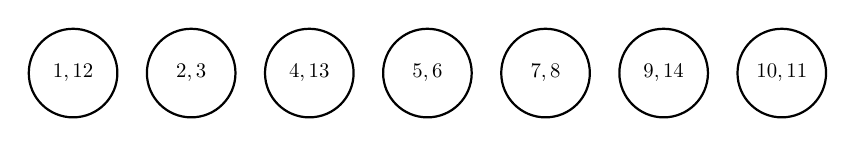
\begin{tikzpicture}[scale=0.75, transform shape, node distance=2cm, state/.style={circle, draw, minimum size=1.5cm}]
        \node[state] (A) [thick] {$\boldsymbol{1, 12}$};
        \node[state] (B) [thick, right of=A] {$\boldsymbol{2, 3}$};
        \node[state] (C) [thick, right of=B] {$\boldsymbol{4, 13}$};
        \node[state] (D) [thick, right of=C] {$\boldsymbol{5, 6}$};
        \node[state] (E) [thick, right of=D] {$\boldsymbol{7, 8}$};
        \node[state] (F) [thick, right of=E] {$\boldsymbol{9, 14}$};
        \node[state] (G) [thick, right of=F] {$\boldsymbol{10, 11}$};
        \path;
\end{tikzpicture}
\caption{\textsc{Resultierende Item-Paare}.}
\label{fig:item_pairs_example_b=3}
\end{figure}

Nachdem die in Abb. \ref{fig:item_pairs_example_b=3} dargestellten Paare von Items generiert wurden, geht es darum,
möglichst viele dieser Paare zu Tripeln von Items zu \textquote{mergen}. Zunächst muss allerdings basierend auf dem entwickelten Rating-System entschieden werden, welche der Paare dazu wieder separiert werden. Durch die Bewertung und anschließende Sortierung der Paare ergeben sich die Abb. \ref{fig:lists_of_pairs} zu entnehmenden unterschiedlich
sortierten Listen.
\begin{figure}[H]
\begin{gather*}
  [(2, 3), (4, 13), (10, 11), (9, 14), (7, 8), (5, 6), (1, 12)] \\
  [(10, 11), (9, 14), (7, 8), (5, 6), (4, 13), (2, 3), (1, 12)] \\
  [(2, 3), (10, 11), (9, 14), (7, 8), (5, 6), (4, 13), (1, 12)]
\end{gather*}
\caption{\textsc{Unterschiedlich sortierte Listen der Item-Paare}.}
\label{fig:lists_of_pairs}
\end{figure}
Es ergeben sich dabei, in zuvor beschriebener Weise, $13$ potenziell unterschiedlich sortierte Listen von Item-Paaren.
In diesem Fall entstehen u.a. aufgrund der geringen Anzahl an Paaren jedoch lediglich drei voneinander unterschiedliche
Sortierungen (vgl. Abb. \ref{fig:lists_of_pairs}).
Anschließend geht es darum, die ersten $\floor{\frac{7}{3.4}} = 2$ Paare zu separieren und möglichst sämtliche der dabei entstehenden Items den verbleibenden Paaren zuzuweisen. Für die erste der drei unterschiedlichen Sortierungen aus Abb. \ref{fig:lists_of_pairs} ergibt sich dabei die in Abb. \ref{fig:pre_merge_step} dargestellte Aufteilung in Paare, welche separiert werden (vgl. Abb. \ref{fig:split_pairs}) und jene, denen die daraus resultierenden Items zugewiesen werden sollen,
um Item-Tripel zu bilden (vgl. Abb. \ref{fig:assign_pairs}).

\vfill
\pagebreak

\begin{figure}[H]
\centering
\begin{subfigure}[b]{\textwidth}
\centering
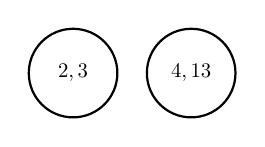
\begin{tikzpicture}[scale=0.75, transform shape, node distance=2cm, state/.style={circle, draw, minimum size=1.5cm}]
        \node[state] (A) [thick] {$\boldsymbol{2, 3}$};
        \node[state] (B) [thick, right of=A] {$\boldsymbol{4, 13}$};
        \path;
\end{tikzpicture}
\caption{\textsc{Split-Pairs}.}
\label{fig:split_pairs}
\end{subfigure}
\begin{subfigure}[b]{\textwidth}
\centering
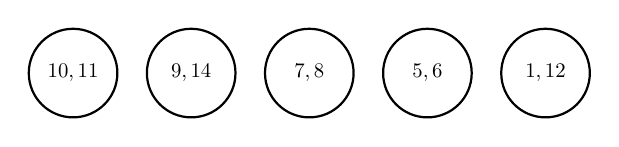
\begin{tikzpicture}[scale=0.75, transform shape, node distance=2cm, state/.style={circle, draw, minimum size=1.5cm}]
        \node[state] (A) [thick] {$\boldsymbol{10, 11}$};
        \node[state] (B) [thick, right of=A] {$\boldsymbol{9, 14}$};
        \node[state] (C) [thick, right of=B] {$\boldsymbol{7, 8}$};
        \node[state] (D) [thick, right of=C] {$\boldsymbol{5, 6}$};
        \node[state] (E) [thick, right of=D] {$\boldsymbol{1, 12}$};
        \path;
\end{tikzpicture}
\caption{\textsc{Assign-Pairs}.}
\label{fig:assign_pairs}
\end{subfigure}
\caption{\textsc{Merge Vorbereitung}.}
\label{fig:pre_merge_step}
\end{figure}

Zwecks Zuweisung der aus der Separation der Paare aus Abb. \ref{fig:split_pairs} hervorgehenden einzelnen
Items $2, 3, 4$ und $13$ zu den verbleibenden Paaren aus Abb. \ref{fig:assign_pairs}, um Tripel zu bilden, wird der in Abb.
\ref{fig:bipartite_graph_pairs_and_unmatched} dargestellte bipartite Graph generiert, welcher die Paare in der einen Partition
und die einzelnen Items in der anderen Partition enthält. Eine Kante zwischen einem einzelnen Item und einem Paar bedeutet,
dass dieses Item dem Paar zugeordnet werden kann, sodass ein kompatibles Tripel entsteht.
In Abb. \ref{fig:item_triple_mcm} ist das auf diesem Graphen berechnete \textsc{MCM} in grün dargestellt, in welchem
sämtliche einzelnen Items einem Paar zugewiesen werden. Das Paar $(5, 6)$ wird dabei als einziges Paar nicht verwendet,
um ein Tripel zu bilden und verbleibt dementsprechend als Item-Paar.

\begin{figure}[H]
\centering

\begin{subfigure}[b]{0.4\textwidth}
\centering
\begin{tikzpicture}[scale=0.7, transform shape, node distance=2cm, state/.style={circle, draw, minimum size=1.5cm}]
        \node[state] (A) [thick] {$\boldsymbol{1, 12}$};
        \node[state] (B) [thick, below of=A] {$\boldsymbol{5, 6}$};
        \node[state] (C) [thick, below of=B] {$\boldsymbol{7, 8}$};
        \node[state] (D) [thick, below of =C] {$\boldsymbol{9, 14}$};
        \node[state] (E) [thick, below of=D] {$\boldsymbol{10, 11}$};
        \node[state] (F) [thick, right = 4cm of A] {$\boldsymbol{2}$};
        \node[state] (G) [thick, below of=F] {$\boldsymbol{3}$};
        \node[state] (H) [thick, below of=G] {$\boldsymbol{4}$};
        \node[state] (I) [thick, below of=H] {$\boldsymbol{13}$};
        \path
          (A) edge [thick] node {} (H)

          (C) edge [thick] node {} (F)
          (C) edge [thick] node {} (G)
          (C) edge [thick] node {} (H)

          (D) edge [thick] node {} (F)
          (D) edge [thick] node {} (H)

          (E) edge [thick] node {} (F)
          (E) edge [thick] node {} (G)
          (E) edge [thick] node {} (H)
          (E) edge [thick] node {} (I);
\end{tikzpicture}
\caption{\textsc{Bipartiter Graph}.}
\label{fig:bipartite_graph_pairs_and_unmatched}
\end{subfigure}
\hspace{10pt}
\begin{subfigure}[b]{0.4\textwidth}
\centering
\begin{tikzpicture}[scale=0.7, transform shape, node distance=2cm, state/.style={circle, draw, minimum size=1.5cm}]
        \node[state] (A) [thick] {$\boldsymbol{\textcolor{mygreen}{1, 12}}$};
        \node[state] (B) [thick, below of=A] {$\boldsymbol{\textcolor{red}{5, 6}}$};
        \node[state] (C) [thick, below of=B] {$\boldsymbol{\textcolor{mygreen}{7, 8}}$};
        \node[state] (D) [thick, below of =C] {$\boldsymbol{\textcolor{mygreen}{9, 14}}$};
        \node[state] (E) [thick, below of=D] {$\boldsymbol{\textcolor{mygreen}{10, 11}}$};
        \node[state] (F) [thick, right = 4cm of A] {$\boldsymbol{\textcolor{mygreen}{2}}$};
        \node[state] (G) [thick, below of=F] {$\boldsymbol{\textcolor{mygreen}{3}}$};
        \node[state] (H) [thick, below of=G] {$\boldsymbol{\textcolor{mygreen}{4}}$};
        \node[state] (I) [thick, below of=H] {$\boldsymbol{\textcolor{mygreen}{13}}$};
        \path
          (A) edge [thick, mygreen] node {} (H)

          (C) edge [thick] node {} (F)
          (C) edge [thick, mygreen] node {} (G)
          (C) edge [thick] node {} (H)

          (D) edge [thick, mygreen] node {} (F)
          (D) edge [thick] node {} (H)

          (E) edge [thick] node {} (F)
          (E) edge [thick] node {} (G)
          (E) edge [thick] node {} (H)
          (E) edge [thick, mygreen] node {} (I);
\end{tikzpicture}
\caption{\textsc{MCM}.}
\label{fig:item_triple_mcm}
\end{subfigure}

\caption{\textsc{Item-Tripel Generierung.}}
\label{fig:item_triple_generation}
\end{figure}

Abbildung \ref{fig:merge_result} zeigt das Ergebnis des Merge-Prozesses, in welchem durch das
\textsc{MCM}, zusätzlich zum verbleibenden Item-Paar, vier Item-Tripel generiert wurden.
\begin{figure}[H]
\centering
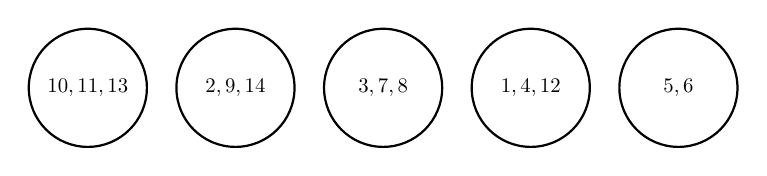
\begin{tikzpicture}[scale=0.75, transform shape, node distance=2.5cm, state/.style={circle, draw, minimum size=2cm}]
        \node[state] (A) [thick] {$\boldsymbol{10, 11, 13}$};
        \node[state] (B) [thick, right of=A] {$\boldsymbol{2, 9, 14}$};
        \node[state] (C) [thick, right of=B] {$\boldsymbol{3, 7, 8}$};
        \node[state] (D) [thick, right of=C] {$\boldsymbol{1, 4, 12}$};
        \node[state] (E) [thick, right of=D] {$\boldsymbol{5, 6}$};
        \path;
\end{tikzpicture}
\caption{\textsc{Merge-Ergebnis.}}
\label{fig:merge_result}
\end{figure}

\vfill
\pagebreak

Die in Abb. \ref{fig:merge_result} dargestellten Item-Tripel sowie das Item-Paar, werden im Folgenden
möglichst günstig und in einer Weise, welche die Placement-Constraints respektiert, einem Stack zugewiesen.
Dazu wird zunächst der vollständig bipartite Graph, welcher in Abb. \ref{fig:complete_bipartite} dargestellt ist,
generiert. Dieser Graph enthält die Items, bestehend aus vier Tripeln und einem Paar, in der einen Partition
und die Stacks in der anderen Partition.
Da es lediglich $5$ Item-Tupel bei $6$ zur Verfügung stehenden Stacks gibt und somit die Partitionen nicht dieselbe
Größe besitzen, wird ein Dummy-Item $D_1$ eingeführt.
Die Kantengewichte sind der Übersichtlichkeit halber nicht in der Darstellung aufgetragen, sondern stattdessen
der Tabelle in Abb. \ref{fig:item_tuple_costs_three_cap} zu entnehmen.
\begin{figure}[H]
\centering
\resizebox{0.7\textwidth}{!}{
\begin{tabular}{| c | c | c | c | c | c | c |}
    \hline
     & $\boldsymbol{S_1}$ & $\boldsymbol{S_2}$ & $\boldsymbol{S_3}$ & $\boldsymbol{S_4}$ & $\boldsymbol{S_5}$ & $\boldsymbol{S_6}$ \\ \hline
    $\boldsymbol{(1, 12, 4)}$ & $128.76$ & $\infty$ & $\infty$ & $\infty$ & $\infty$ & $\infty$ \\ \hline
    $\boldsymbol{(7, 8, 3)}$ & $134.82$ & $\infty$ & $98.46$ & $\infty$ & $\infty$ & $80.28$ \\ \hline
    $\boldsymbol{(9, 14, 2)}$ & $\infty$ & $159.06$ & $\infty$ & $146.94$ & $\infty$ & $134.82$ \\ \hline
    $\boldsymbol{(10, 11, 13)}$ & $231.78$ & $\infty$ & $195.42$ & $\infty$ & $159.06$ & $140.88$ \\ \hline
    $\boldsymbol{(5, 6)}$ & $83.82$ & $71.7$ & $59.58$ & $\infty$ & $35.34$ & $\infty$ \\ \hline
    $\boldsymbol{D_1}$ & $0.0$ & $0.0$ & $0.0$ & $0.0$ & $0.0$ & $0.0$ \\ \hline
\end{tabular}}
\caption{\textsc{Kosten der Stack-Zuweisungen}.}
\label{fig:item_tuple_costs_three_cap}
\end{figure}

Anschließend wird im bipartiten Graphen aus Abb. \ref{fig:complete_bipartite} das \textsc{MWPM} berechnet, welches
in Abb. \ref{fig:mwpm} dargestellt ist und einer günstigsten Zuweisung der zuvor generierten Item-Tupel zu den Stacks entspricht.

\begin{figure}[H]
% \begin{figure}[H]
\begin{subfigure}[b]{0.4\textwidth}
\centering
\begin{tikzpicture}[scale=0.45, transform shape, node distance=2.5cm, state/.style={circle, draw, minimum size=2.25cm}]
        \node[state] (A) [thick] {$\boldsymbol{1, 12, 4}$};
        \node[state] (B) [thick, below of=A] {$\boldsymbol{7, 8, 3}$};
        \node[state] (C) [thick, below of=B] {$\boldsymbol{9, 14, 2}$};
        \node[state] (D) [thick, below of=C] {$\boldsymbol{10, 11, 13}$};
        \node[state] (E) [thick, below of=D] {$\boldsymbol{5, 6}$};
        \node[state] (F) [thick, below of=E] {$\boldsymbol{D_1}$};

        \node[state] (G) [thick, right = 5cm of A] {$\boldsymbol{S_1}$};
        \node[state] (H) [thick, below of=G] {$\boldsymbol{S_2}$};
        \node[state] (I) [thick, below of=H] {$\boldsymbol{S_3}$};
        \node[state] (J) [thick, below of=I] {$\boldsymbol{S_4}$};
        \node[state] (K) [thick, below of=J] {$\boldsymbol{S_5}$};
        \node[state] (L) [thick, below of=K] {$\boldsymbol{S_6}$};

        \path
          (A) edge [thick] node {} (G)
          (A) edge [thick] node {} (H)
          (A) edge [thick] node {} (I)
          (A) edge [thick] node {} (J)
          (A) edge [thick] node {} (K)
          (A) edge [thick] node {} (L)

          (B) edge [thick] node {} (G)
          (B) edge [thick] node {} (H)
          (B) edge [thick] node {} (I)
          (B) edge [thick] node {} (J)
          (B) edge [thick] node {} (K)
          (B) edge [thick] node {} (L)

          (C) edge [thick] node {} (G)
          (C) edge [thick] node {} (H)
          (C) edge [thick] node {} (I)
          (C) edge [thick] node {} (J)
          (C) edge [thick] node {} (K)
          (C) edge [thick] node {} (L)

          (D) edge [thick] node {} (G)
          (D) edge [thick] node {} (H)
          (D) edge [thick] node {} (I)
          (D) edge [thick] node {} (J)
          (D) edge [thick] node {} (K)
          (D) edge [thick] node {} (L)

          (E) edge [thick] node {} (G)
          (E) edge [thick] node {} (H)
          (E) edge [thick] node {} (I)
          (E) edge [thick] node {} (J)
          (E) edge [thick] node {} (K)
          (E) edge [thick] node {} (L)

          (F) edge [thick] node {} (G)
          (F) edge [thick] node {} (H)
          (F) edge [thick] node {} (I)
          (F) edge [thick] node {} (J)
          (F) edge [thick] node {} (K)
          (F) edge [thick] node {} (L);
\end{tikzpicture}
\caption{\textsc{Vollständig Bipartit}.}
\label{fig:complete_bipartite}
\end{subfigure}
\hfill
\begin{subfigure}[b]{0.4\textwidth}
\centering
\begin{tikzpicture}[scale=0.45, transform shape, node distance=2.5cm, state/.style={circle, draw, minimum size=2.25cm}]
        \node[state] (A) [thick] {$\boldsymbol{1, 12, 4}$};
        \node[state] (B) [thick, below of=A] {$\boldsymbol{7, 8, 3}$};
        \node[state] (C) [thick, below of=B] {$\boldsymbol{9, 14, 2}$};
        \node[state] (D) [thick, below of=C] {$\boldsymbol{10, 11, 13}$};
        \node[state] (E) [thick, below of=D] {$\boldsymbol{5, 6}$};
        \node[state] (F) [thick, below of=E] {$\boldsymbol{D_1}$};

        \node[state] (G) [thick, right = 5cm of A] {$\boldsymbol{S_1}$};
        \node[state] (H) [thick, below of=G] {$\boldsymbol{S_2}$};
        \node[state] (I) [thick, below of=H] {$\boldsymbol{S_3}$};
        \node[state] (J) [thick, below of=I] {$\boldsymbol{S_4}$};
        \node[state] (K) [thick, below of=J] {$\boldsymbol{S_5}$};
        \node[state] (L) [thick, below of=K] {$\boldsymbol{S_6}$};

        \path
          (A) edge [thick, above] node {$128.76$} (G)
          (B) edge [thick, above right, near start] node {$98.46$} (I)
          (C) edge [thick, near start, above right] node {$146.94$} (J)
          (D) edge [thick, below left, near end] node {$140.88$} (L)
          (E) edge [thick, near end, above] node {$35.34$} (K)
          (F) edge [thick, below right] node {$0.0$} (H);
\end{tikzpicture}
\caption{\textsc{MWPM}.}
\label{fig:mwpm}
\end{subfigure}
\caption{\textsc{Stack-Zuweisung}.}
\label{}
\end{figure}

Da keine Kante im \textsc{MWPM} das Gewicht $\infty$ besitzt, handelt es sich um eine günstigste, zulässige Zuweisung
sämtlicher Item-Tupel zu Stacks, welche insgesamt die Kosten $550.38$ verursacht.
Die daraus resultierende Stacking-Lösung ist in Abb. \ref{fig:valid_solution} dargestellt, wobei die Reihenfolge
innerhalb der Stacks ggf. in zuvor beschriebener Weise angepasst werden muss.

\vfill
\pagebreak

\begin{figure}[H]
  \centering
  \resizebox{0.4\textwidth}{!}{
    \begin{tabular}{c|c|c|c|c|c|c|}
    \cline{2-7}
    $\boldsymbol{L_3}$ & $4$ & $$ & $3$ & $2$ & $$ & $13$ \\ \cline{2-7}
    $\boldsymbol{L_2}$ & $12$ & $$ & $8$ & $14$ & $6$ & $11$\\ \cline{2-7}
    $\boldsymbol{L_1}$ & $1$ & $$ & $7$ & $9$ & $5$ & $10$ \\ \cline{2-7}
    \multicolumn{1}{c}{} & \multicolumn{1}{c}{$\boldsymbol{S_1}$} & \multicolumn{1}{c}{$\boldsymbol{S_2}$}
    & \multicolumn{1}{c}{$\boldsymbol{S_3}$} & \multicolumn{1}{c}{$\boldsymbol{S_4}$} & \multicolumn{1}{c}{$\boldsymbol{S_5}$}
    & \multicolumn{1}{c}{$\boldsymbol{S_6}$} \\
    \end{tabular}}
    \caption{\textsc{Zulässige Zuweisungen.}}
    \label{fig:valid_solution}
\end{figure}

Diese Lösung basiert auf der ersten der drei unterschiedlichen Sortierungen der Item-Paare aus Abb. \ref{fig:lists_of_pairs}.
Um die bestmögliche Lösung zu finden, wird der geschilderte Prozess für die beiden übrigen Sortierungen
ebenfalls durchgeführt und schließlich eine beste Lösung in Bezug auf die Kosten ausgewählt.

Ist der Postprocessing-Schritt aktiviert, so wird zuletzt die beste generierte Lösung erneut betrachtet
und es werden ausgewählte Items an freie Positionen in anderen Stacks verschoben, sofern sich dadurch eine
Kostenersparnis ergibt.
Dazu wird der bipartite Postprocessing-Graph generiert, welcher in Abb. \ref{fig:post_processing_graph_b=3} dargestellt ist.
Dieser enthält die Items in der einen Partition und die freien Positionen innerhalb der Stacks in der anderen Partition.
Die Positionen sind erneut jeweils in der Notation $pos(stackIdx, level)$ gegeben. In diesem Beispiel gibt es,
wie man Abb. \ref{fig:valid_solution} entnehmen kann, mit $pos(2, 1)$, $pos(2, 2)$, $pos(2, 3)$ und $pos(5, 3)$
vier verbleibende freie Positionen in den Stacks. Die Kantengewichte des Postprocessing-Graphen sind der Übersichtlichkeit halber nicht an den Kanten notiert, sondern in der Tabelle in Abb. \ref{fig:post_processing_costs} aufgeführt.

\begin{figure}[H]
\centering
\begin{tikzpicture}[scale=0.5, transform shape, node distance=2.25cm, state/.style={circle, draw, minimum size=1cm}]
        \node[state] (A) [thick] {$\boldsymbol{1}$};
        \node[state] (B) [thick, right of=A] {$\boldsymbol{2}$};
        \node[state] (C) [thick, right of=B] {$\boldsymbol{3}$};
        \node[state] (D) [thick, right of=C] {$\boldsymbol{4}$};
        \node[state] (E) [thick, right of=D] {$\boldsymbol{5}$};
        \node[state] (F) [thick, right of=E] {$\boldsymbol{6}$};
        \node[state] (G) [thick, right of=F] {$\boldsymbol{7}$};
        \node[state] (H) [thick, right of=G] {$\boldsymbol{8}$};
        \node[state] (I) [thick, right of=H] {$\boldsymbol{9}$};
        \node[state] (J) [thick, right of=I] {$\boldsymbol{10}$};
        \node[state] (K) [thick, right of=J] {$\boldsymbol{11}$};
        \node[state] (L) [thick, right of=K] {$\boldsymbol{12}$};
        \node[state] (M) [thick, right of=L] {$\boldsymbol{13}$};
        \node[state] (N) [thick, right of=M] {$\boldsymbol{14}$};

        \node[state] (O) [thick, below = 5cm of B] {$\boldsymbol{pos(2, 1)}$};
        \node[state] (P) [thick, below = 5cm of F] {$\boldsymbol{pos(2, 2)}$};
        \node[state] (Q) [thick, below = 5cm of I] {$\boldsymbol{pos(2, 3)}$};
        \node[state] (R) [thick, below = 5cm of M] {$\boldsymbol{pos(5, 3)}$};

        \path
            (B) edge [thick] node {$$} (O)
            (B) edge [thick] node {$$} (P)
            (B) edge [thick] node {$$} (Q)
            (D) edge [thick] node {$$} (O)
            (D) edge [thick] node {$$} (P)
            (D) edge [thick] node {$$} (Q)
            (E) edge [thick] node {$$} (O)
            (E) edge [thick] node {$$} (P)
            (E) edge [thick] node {$$} (Q)
            (E) edge [thick] node {$$} (R)
            (F) edge [thick] node {$$} (O)
            (F) edge [thick] node {$$} (P)
            (F) edge [thick] node {$$} (Q)
            (F) edge [thick] node {$$} (R)
            (H) edge [thick] node {$$} (O)
            (H) edge [thick] node {$$} (P)
            (H) edge [thick] node {$$} (Q)
            (I) edge [thick] node {$$} (O)
            (I) edge [thick] node {$$} (P)
            (I) edge [thick] node {$$} (Q)
            (J) edge [thick] node {$$} (O)
            (J) edge [thick] node {$$} (P)
            (J) edge [thick] node {$$} (Q)
            (K) edge [thick] node {$$} (O)
            (K) edge [thick] node {$$} (P)
            (K) edge [thick] node {$$} (Q)
            (L) edge [thick] node {$$} (O)
            (L) edge [thick] node {$$} (P)
            (L) edge [thick] node {$$} (Q)
            (L) edge [thick] node {$$} (R)
            (N) edge [thick] node {$$} (O)
            (N) edge [thick] node {$$} (P)
            (N) edge [thick] node {$$} (Q);
\end{tikzpicture}
\caption{\textsc{Postprocessing-Graph}.}
\label{fig:post_processing_graph_b=3}
\end{figure}

Wie man der Tabelle in Abb. \ref{fig:post_processing_costs} entnehmen kann, sind im Gegensatz zum Beispiel
der Heuristik aus Abschnitt \ref{sec:two_cap_heuristic} in diesem Fall positive Kantengewichte vorhanden,
was bedeutet, dass sich durch Verschieben ausgewählter Items an freie Positionen Kosten einsparen lassen.

\vfill
\pagebreak

\begin{figure}[H]
\centering
\resizebox{0.5\textwidth}{!}{
\begin{tabular}{| c | c | c | c | c |}
    \hline
     & $\boldsymbol{pos(2, 1)}$ & $\boldsymbol{pos(2, 2)}$ & $\boldsymbol{pos(2, 3)}$ & $\boldsymbol{pos(5, 3)}$ \\ \hline
     $2$ & $12.12$ & $12.12$ & $12.12$ & $-$ \\ \hline
     $4$ & $6.06$ & $6.06$ & $6.06$ & $-$ \\ \hline
     $5$ & $-18.18$ & $-18.18$ & $-18.18$ & $0.0$ \\ \hline
     $6$ & $-18.18$ & $-18.18$ & $-18.18$ & $0.0$ \\ \hline
     $8$ & $-6.06$ & $-6.06$ & $-6.06$ & $-$ \\ \hline
     $9$ & $-12.12$ & $-12.12$ & $-12.12$ & $-$ \\ \hline
     $10$ & $-24.24$ & $-24.24$ & $-24.24$ & $-$ \\ \hline
     $11$ & $-24.24$ & $-24.24$ & $-24.24$ & $-$ \\ \hline
     $12$ & $6.06$ & $6.06$ & $6.06$ & $24.24$ \\ \hline
     $14$ & $-12.12$ & $-12.12$ & $-12.12$ & $-$ \\ \hline
\end{tabular}}
\caption{\textsc{Kantengewichte des Postprocessing-Graphen}.}
\label{fig:post_processing_costs}
\end{figure}

Jene Zuordnungen von Items zu freien Positionen, welche zur insgesamt größten Kostenreduktion führen, werden durch
das Maximum-Weight-Bipartite-Matching im Graphen aus Abb. \ref{fig:post_processing_graph_b=3} ermittelt,
welches in Abb. \ref{fig:mwbm} dargestellt ist.
Diese Zuordnungen sorgen für eine Gesamtersparnis von $36.36$, welche sich wie folgt ergibt.
Item $12$ wird mit einer Ersparnis von $24.24$ in $S_5$ platziert. Da die Items $2$ und $4$ beide $S_2$ zugeordnet werden,
wird lediglich das Item mit der größeren Ersparnis verschoben. Somit wird Item $2$ mit einer Ersparnis von $12.12$
in $S_2$ platziert. Insgesamt verringern sich die Kosten der Lösung von $550.38$ auf $514.02$.

\begin{figure}[H]
\centering
\begin{tikzpicture}[scale=0.5, transform shape, node distance=1.5cm, state/.style={circle, draw, minimum size=1.25cm}]
        \node[state] (A) [thick] {$\boldsymbol{1}$};
        \node[state] (B) [thick, right of=A] {$\boldsymbol{2}$};
        \node[state] (C) [thick, right of=B] {$\boldsymbol{3}$};
        \node[state] (D) [thick, right of=C] {$\boldsymbol{4}$};
        \node[state] (E) [thick, right of=D] {$\boldsymbol{5}$};
        \node[state] (F) [thick, right of=E] {$\boldsymbol{6}$};
        \node[state] (G) [thick, right of=F] {$\boldsymbol{7}$};
        \node[state] (H) [thick, right of=G] {$\boldsymbol{8}$};
        \node[state] (I) [thick, right of=H] {$\boldsymbol{9}$};
        \node[state] (J) [thick, right of=I] {$\boldsymbol{10}$};
        \node[state] (K) [thick, right of=J] {$\boldsymbol{11}$};
        \node[state] (L) [thick, right of=K] {$\boldsymbol{12}$};
        \node[state] (M) [thick, right of=L] {$\boldsymbol{13}$};
        \node[state] (N) [thick, right of=M] {$\boldsymbol{14}$};

        \node[state] (O) [thick, below = 2cm of B] {$\boldsymbol{pos(2, 1)}$};
        \node[state] (P) [thick, below = 2cm of F] {$\boldsymbol{pos(2, 2)}$};
        \node[state] (Q) [thick, below = 2cm of I] {$\boldsymbol{pos(2, 3)}$};
        \node[state] (R) [thick, below = 2cm of M] {$\boldsymbol{pos(5, 3)}$};

        \path
            (B) edge [thick, left] node {$12.12$} (O)
            (D) edge [thick, right] node {$6.06$} (P)
            (L) edge [thick, right] node {$24.24$} (R);
\end{tikzpicture}
\caption{\textsc{Maximum-Weight-Bipartite-Matching}.}
\label{fig:mwbm}
\end{figure}

In Abb. \ref{fig:valid_solution_post_processing} ist das finale Ergebnis zu sehen, in welchem
die im Zuge des Postprocessings verschobenen Items in grün dargestellt sind.
Zuletzt muss ggf. in zuvor beschriebener Weise die Reihenfolge innerhalb der Stacks angepasst werden,
sodass sie den Stacking-Constraints entspricht. Da es sich beim Postprocessing um ein iteratives Verfahren handelt,
würde dieser Prozess nun wiederholt, bis sich keine Verbesserung der Lösung mehr erzielen lässt.
In diesem Beispiel wird bereits nach der ersten Iteration das beste Ergebnis erzielt und der Postprocessing-Prozess terminiert.

\begin{figure}[H]
  \centering
  \resizebox{0.4\textwidth}{!}{
    \begin{tabular}{c|c|c|c|c|c|c|}
    \cline{2-7}
    $\boldsymbol{L_3}$ & $$ & $$ & $3$ & $$ & $\textcolor{mygreen}{12}$ & $13$ \\ \cline{2-7}
    $\boldsymbol{L_2}$ & $4$ & $$ & $8$ & $14$ & $6$ & $11$\\ \cline{2-7}
    $\boldsymbol{L_1}$ & $1$ & $\textcolor{mygreen}{2}$ & $7$ & $9$ & $5$ & $10$ \\ \cline{2-7}
    \multicolumn{1}{c}{} & \multicolumn{1}{c}{$\boldsymbol{S_1}$} & \multicolumn{1}{c}{$\boldsymbol{S_2}$}
    & \multicolumn{1}{c}{$\boldsymbol{S_3}$} & \multicolumn{1}{c}{$\boldsymbol{S_4}$} & \multicolumn{1}{c}{$\boldsymbol{S_5}$}
    & \multicolumn{1}{c}{$\boldsymbol{S_6}$} \\
    \end{tabular}}
    \caption{\textsc{Postprocessing-Ergebnis.}}
    \label{fig:valid_solution_post_processing}
\end{figure}

\vfill
\pagebreak

\subsection{Vergleich der Solver für $b = 3$}
\label{sec:solver_comp_b=3}

In diesem Abschnitt werden die verschiedenen Solver für Instanzen von Stacking-Problemen mit einer Stack-Kapazität
von $b = 3$ miteinander verglichen. Dabei gilt weiterhin das in Abschnitt \ref{sec:solver_comp_b=2} vorgestellte Setup
bezüglich der Vergleichskategorien, der \textsc{CPLEX}-Konfiguration sowie der verwendeten Hardware.

Der in Abschnitt \ref{sec:three_cap_heuristic} eingeführte Parameter \textit{prioritizeRuntime} zur Konfiguration der Heuristik
wird in den folgenden Experimenten stets auf \textit{false} gesetzt, weil die durch Verwendung des Rating-Systems erhöhten Laufzeiten
aus praktischer Perspektive vermutlich in jedem Fall vertretbar sind. Aufgrunddessen liegt der Fokus hier auf dem Erreichen
möglichst geringer Zielfunktionswerte. Liegt der Fokus in der Praxis hingegen auf einer möglichst geringen Laufzeit, so kann dementsprechend \textit{prioritizeRuntime} auf \textit{true} gesetzt werden, was zu erheblich kürzeren Laufzeiten bei nur geringfügig schlechteren Zielfunktionswerten führt.
Des Weiteren wird der ebenfalls in Abschnitt \ref{sec:three_cap_heuristic} eingeführte Parameter \textit{postProcessing}
stets auf \textit{true} gesetzt, damit, wie bereits bei der Heuristik zur Lösung von Instanzen mit Stacks der Kapazität $b = 2$,
ein reiner Fokus auf Kostenminimierung besteht, welcher eine Vergleichbarkeit mit den MIP-Formulierungen erlaubt, die ebenfalls
ausschließlich Kosten minimieren.

\textbf{Kleine Instanzen (s)}

Zunächst zum experimentellen Vergleich der Solver für kleine Instanzen, bei denen es darum geht,
$100$ eintreffende Items in die Storage-Area zu verladen.

In Abb. \ref{fig:instance_coverage_b=3_s} ist die Instance-Coverage der einzelnen Solver bei einem Zeitlimit von $0.5s, 1s$ und $2s$ pro Instanz dargestellt. Die Heuristik wird in den folgenden Diagrammen analog zur Heuristik für $b = 2$ stets mit \textsc{3Cap} abgekürzt. Die Bin-Packing-Formulierung, welche bereits bei einem Zeitlimit von $0.5s$ zu einer Instance-Coverage von $80 \%$ gelangt, ist in dieser Kategorie offensichtlich schneller als die 3-Index-Formulierung, welche bei diesem Zeitlimit keine Instanz zulässig löst (vgl. Abb. \ref{fig:instance_coverage_b=3_s_a}).
Grundsätzlich gilt allerdings, wie Abb. \ref{fig:instance_coverage_b=3_s_b} zu entnehmen ist, dass sämtliche Solver
bei einem vergleichsweise geringen Zeitlimit von $1s$ alle Instanzen zulässig lösen.
Für die Heuristik sind die Zeitlimits irrelevant, da diese mit einer durchschnittlichen Laufzeit
von $0.1s$ sämtliche Instanzen zulässig löst.

\begin{figure}[H]
\centering

\begin{subfigure}[b]{0.3\textwidth}
\centering
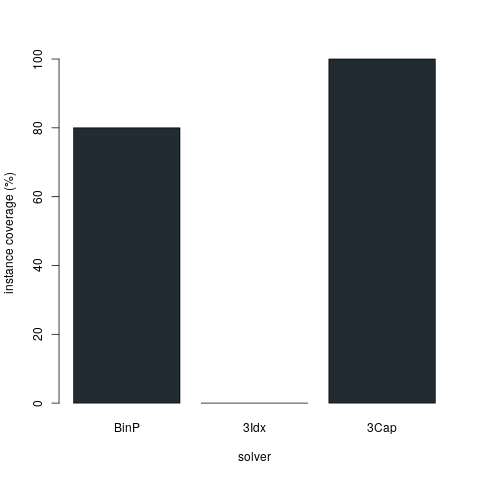
\includegraphics[width=1.1\textwidth]{img/solver_instance_coverage_b=3_s_0_5s.png}
\caption{\textsc{Zeitlimit} $0.5s$}
\label{fig:instance_coverage_b=3_s_a}
\end{subfigure}
\hfill
\begin{subfigure}[b]{0.3\textwidth}
\centering
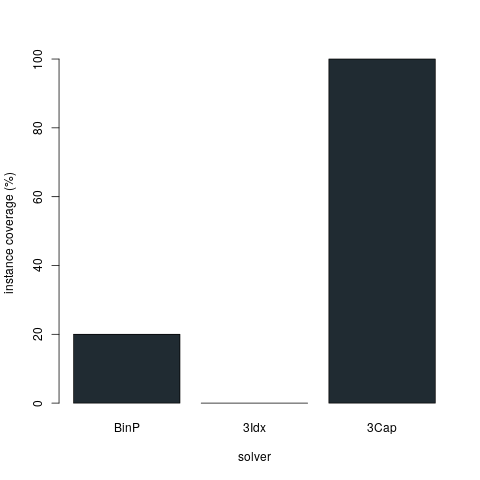
\includegraphics[width=1.1\textwidth]{img/solver_instance_coverage_b=3_s_1s.png}
\caption{\textsc{Zeitlimit} $1s$}
\label{fig:instance_coverage_b=3_s_b}
\end{subfigure}
\hfill
\begin{subfigure}[b]{0.3\textwidth}
\centering
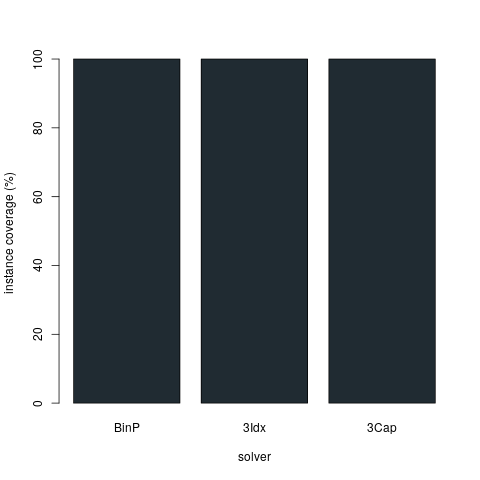
\includegraphics[width=1.1\textwidth]{img/solver_instance_coverage_b=3_s_2s.png}
\caption{\textsc{Zeitlimit} $2s$}
\label{fig:instance_coverage_b=3_s_c}
\end{subfigure}

\caption{\textsc{Instance-Coverage der $b = 3$ Solver (s)}.}
\label{fig:instance_coverage_b=3_s}
\end{figure}

\vfill
\pagebreak

In der Darstellung der Laufzeiten bei einem Zeitlimit von $2s$ in Abb. \ref{fig:b=3_s_runtimes} ist zu erkennen,
dass die Bin-Packing-Formulierung in jedem Fall deutlich schneller ist als die 3-Index-Formulierung, welche bei sämtlichen Instanzen durch das Zeitlimit terminiert. Die Bin-Packing-Formulierung wird wiederum in jedem Fall
von der Heuristik unterboten. Da die absoluten Laufzeitdifferenzen dargestellt sind, ist es wichtig,
zu berücksichtigen, dass die Heuristik beide MIP-Formulierungen deutlich unterbietet, denn zwischen der durchschnittlichen Laufzeit der Heuristik und jener der Bin-Packing-Formulierung besteht ein
Faktor von $11.5$, während zwischen den beiden MIP-Formulierungen lediglich ein Faktor von $1.7$ besteht.
Da die Bin-Packing-Formulierung, wie in Abb. \ref{fig:b=3_s_runtimes} zu erkennen ist, stets vor dem Zeitlimit terminiert, löst diese sämtliche Instanzen optimal. Dass die 3-Index-Formulierung in jedem Fall durch das Zeitlimit gestoppt wird, äußert sich darin, dass diese in keinem Fall den optimalen Zielfunktionswert ermittelt und sämtliche Instanzen nur mit einer erheblichen Abweichung vom Optimum löst (vgl. Abb. \ref{fig:b=3_s_costs}).
Wie bereits in den Experimenten aus Abschnitt \ref{sec:solver_comp_b=2}, wurde auch hier die Darstellung der Kosten
in einer Weise skaliert, welche es ermöglicht, sämtliche Einträge zu erkennen. Die tatsächlichen Abstände können anhand der Beschriftungen auf der $x$-Achse nachvollzogen werden.
Wie man ebenfalls der Abbildung entnehmen kann, gelangt die Heuristik bei jeder Instanz zu erheblich besseren Zielfunktionswerten als die 3-Index-Formulierung. Die Heuristik konnte mit Instanz $00$ sogar eine Instanz optimal lösen, weshalb ihr Eintrag in Abb. \ref{fig:b=3_s_costs} den Eintrag der Bin-Packing-Formulierung verdeckt,
welche ebenfalls den optimalen Zielfunktionswert ermittelt.
Die in Abb. \ref{fig:b=3_s_costs} dargestellten unteren Schranken zeigen, dass die Stacking-Constraints in dieser Kategorie mit den Instanzen $05, 06, 08, 10$ und $15$ in einigen Fällen keinen Einfluss auf den optimalen Zielfunktionswert haben. In vielen weiteren Fällen ist der Einfluss sehr gering und nur in wenigen Fällen, beispielsweise bei den Instanzen $04$ und $11$, fällt dieser deutlich größer aus.

\begin{figure}[H]
\centering
\begin{subfigure}[b]{0.4\textwidth}
\centering
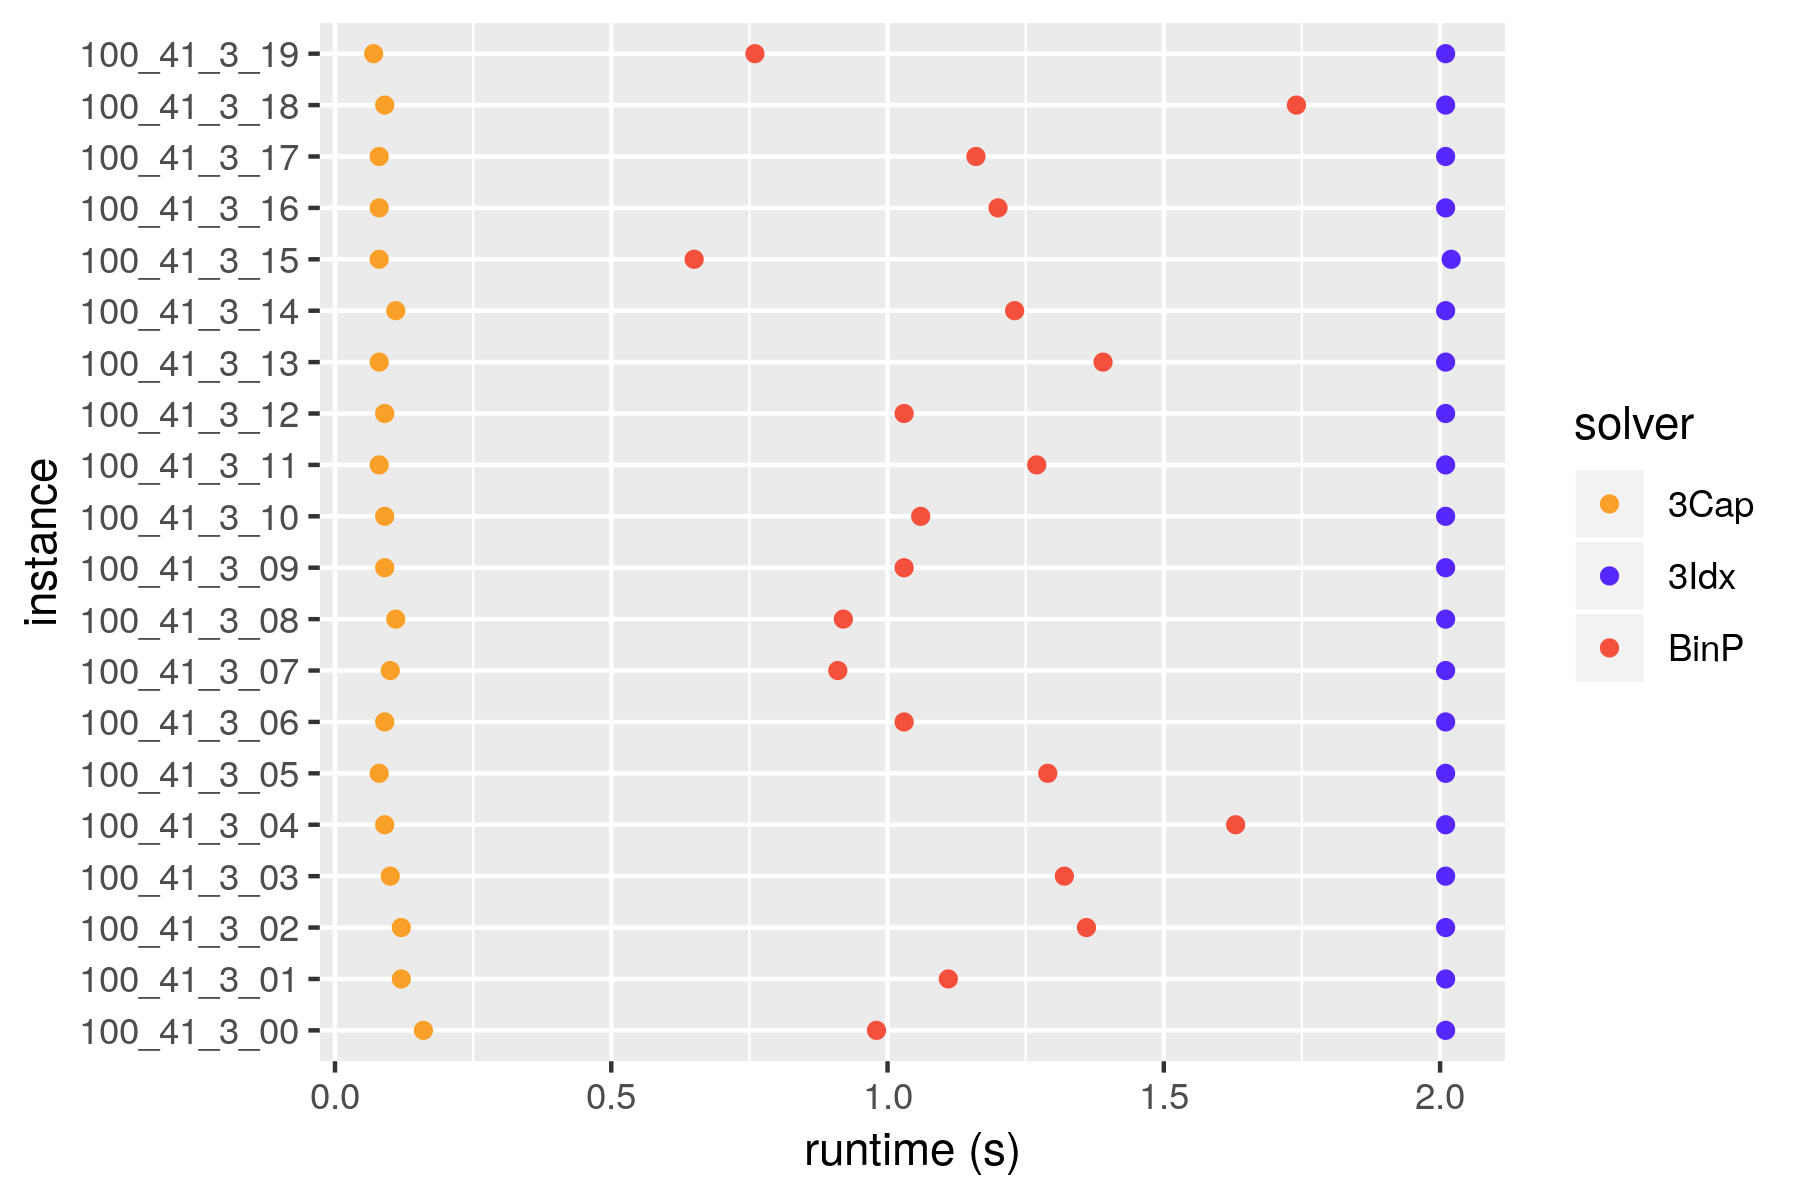
\includegraphics[width=1.3\textwidth]{img/solver_instance_time_b=3_s_2s.png}
\caption{\textsc{Laufzeiten}}
\label{fig:b=3_s_runtimes}
\end{subfigure}
\hfill
\begin{subfigure}[b]{0.4\textwidth}
\centering
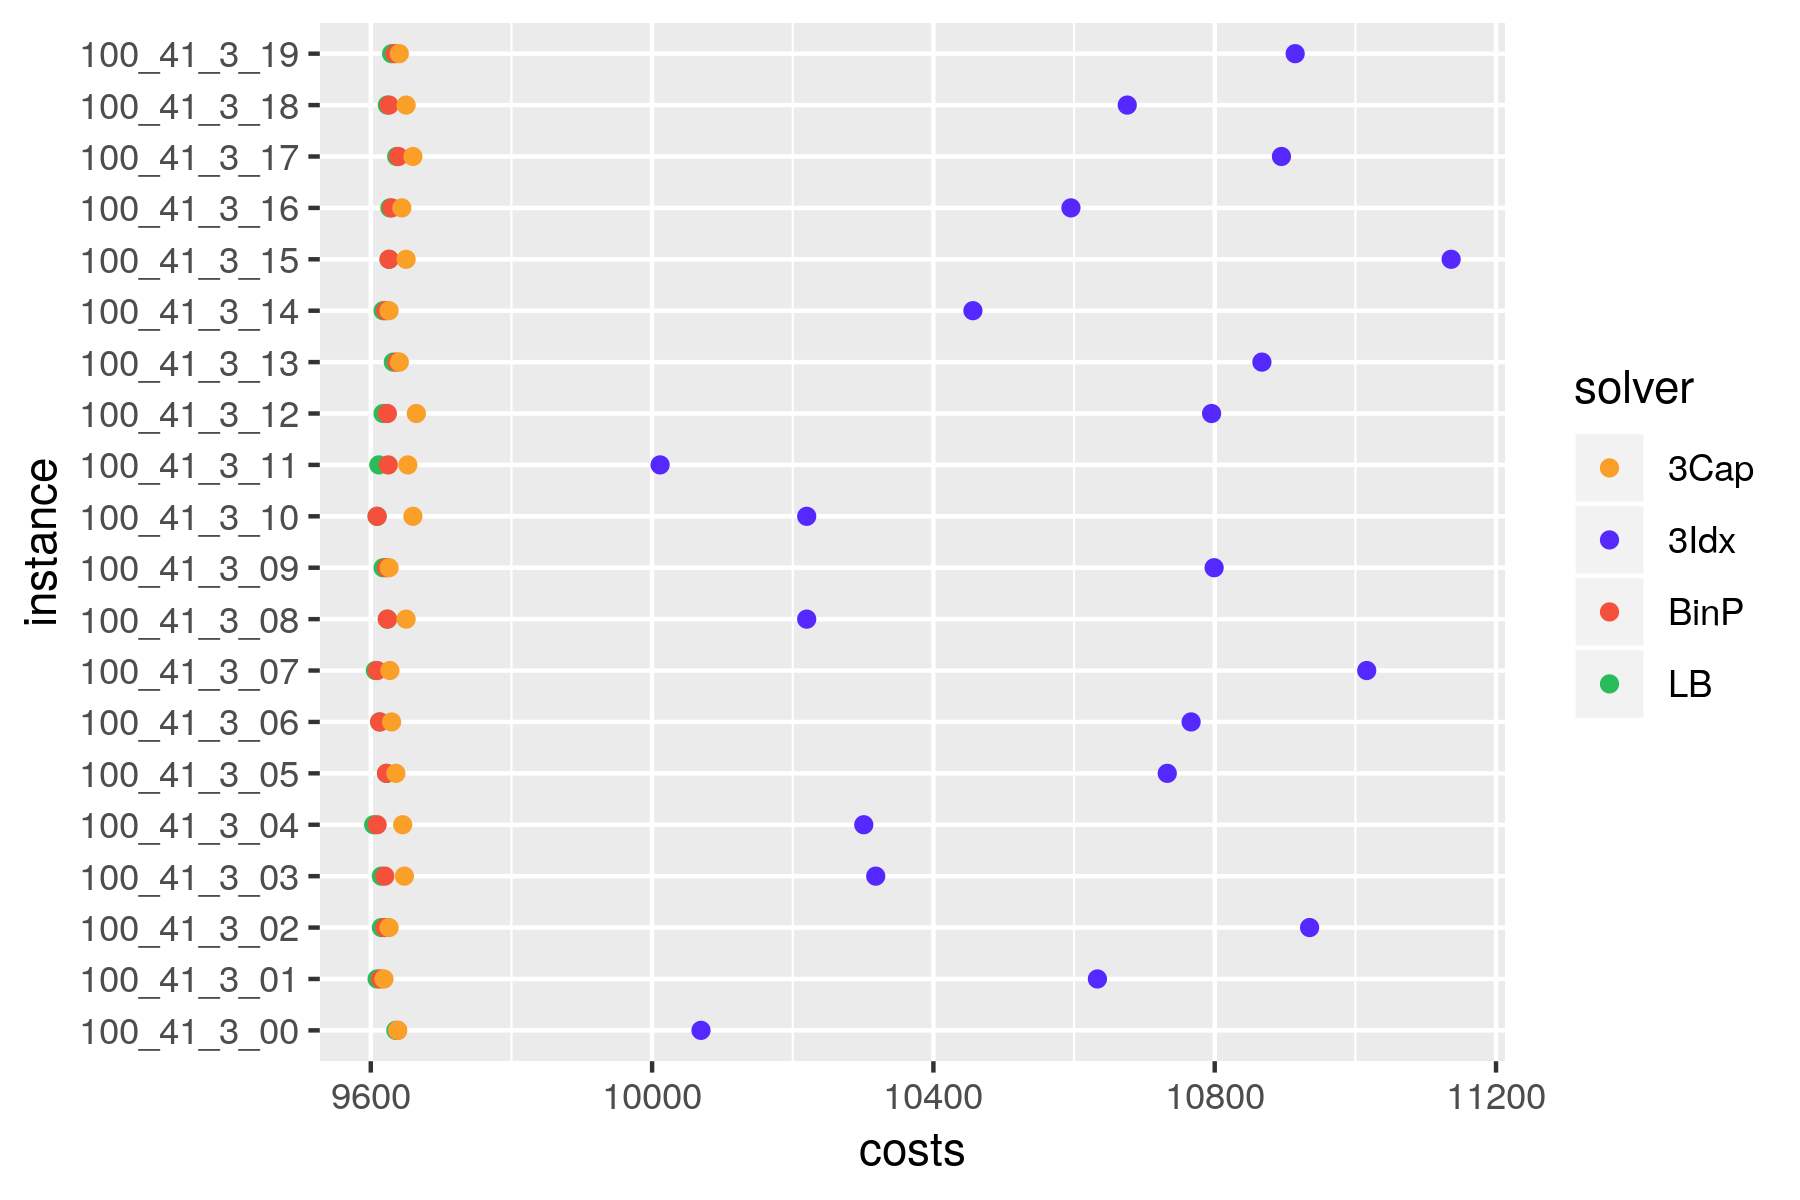
\includegraphics[width=1.3\textwidth]{img/solver_instance_cost_b=3_s_2s.png}
\caption{\textsc{Kosten}}
\label{fig:b=3_s_costs}
\end{subfigure}
\caption{\textsc{Ergebnisse bei $2s$ Zeitlimit}.}
\end{figure}

Die exakten Ergebnisse der MIP-Formulierungen können in den Tabellen in Abb. \ref{fig:mip_results_b=3_s} nachvollzogen werden. Abbildung \ref{fig:mip_results_b=3_s_c} ist zu entnehmen, dass die Bin-Packing-Formulierung nach
durchschnittlich $1.15s$ sämtliche Instanzen optimal löst. Die 3-Index-Formulierung löst bei diesem Zeitlimit keine Instanz optimal und weicht um durchschnittlich $10.34 \%$ vom Optimum ab.
Die Bin-Packing-Formulierung ist der 3-Index-Formulierung somit in dieser Kategorie sehr deutlich überlegen.

\begin{figure}[H]
\centering
\begin{subfigure}[b]{0.3\textwidth}
\centering
\resizebox{\textwidth}{!}{
\begin{tabular}{ | c | c | c |}
    \hline
     & \textbf{BinP} & \textbf{3Idx} \\ \hline
    \textbf{Optimal ($\boldsymbol{\%}$)} & $0$ & $0$ \\ \hline
    \textbf{\O \thinspace Laufzeit ($\boldsymbol{s}$)} & $\textcolor{mygreen}{0.53}$ & $\textcolor{red}{-}$ \\ \hline
    \textbf{\O \thinspace Abweichung ($\boldsymbol{\%}$)} & $\textcolor{mygreen}{15.18}$ & $\textcolor{red}{-}$ \\ \hline
\end{tabular}}
\caption{\textsc{Zeitlimit} $0.5s$}
\label{fig:mip_results_b=3_s_a}
\end{subfigure}
% \end{figure}
% \begin{figure}[H]
\begin{subfigure}[b]{0.3\textwidth}
\centering
\resizebox{\textwidth}{!}{
\begin{tabular}{ | c | c | c |}
    \hline
     & \textbf{BinP} & \textbf{3Idx} \\ \hline
    \textbf{Optimal ($\boldsymbol{\%}$)} & $\textcolor{mygreen}{30}$ & $\textcolor{red}{0}$ \\ \hline
    \textbf{\O \thinspace Laufzeit ($\boldsymbol{s}$)} & $\textcolor{mygreen}{0.98}$ & $\textcolor{red}{1.01}$ \\ \hline
    \textbf{\O \thinspace Abweichung ($\boldsymbol{\%}$)} & $\textcolor{mygreen}{3.15}$ & $\textcolor{red}{10.55}$ \\ \hline
\end{tabular}}
\caption{\textsc{Zeitlimit} $1s$}
\label{fig:mip_results_b=3_s_b}
\end{subfigure}
\begin{subfigure}[b]{0.3\textwidth}
\centering
\resizebox{\textwidth}{!}{
\begin{tabular}{ | c | c | c |}
    \hline
     & \textbf{BinP} & \textbf{3Idx} \\ \hline
    \textbf{Optimal ($\boldsymbol{\%}$)} & $ \textcolor{mygreen}{100}$ & $ \textcolor{red}{0}$ \\ \hline
    \textbf{\O \thinspace Laufzeit ($\boldsymbol{s}$)} & $\textcolor{mygreen}{1.15}$ & $\textcolor{red}{2.01}$ \\ \hline
    \textbf{\O \thinspace Abweichung ($\boldsymbol{\%}$)} & $\textcolor{mygreen}{0.0}$ & $\textcolor{red}{10.34}$ \\ \hline
\end{tabular}}
\caption{\textsc{Zeitlimit} $2s$}
\label{fig:mip_results_b=3_s_c}
\end{subfigure}
\caption{\textsc{MIP-Ergebnisse.}}
\label{fig:mip_results_b=3_s}
\end{figure}

Bei der durchschnittlichen Abweichung der Heuristik von $0.2 \%$ handelt es sich sicher, in Anbetracht
der enormen Laufzeitverbesserung, um einen akzeptablen Wert, allerdings gilt, wie schon in der Kategorie
der kleinen Instanzen für eine Stack-Kapazität von $b = 2$ auch hier, dass die durchschnittlich benötigten $1.15s$
für die exakte Lösung seitens der Bin-Packing-Formulierung aus praktischer Perspektive vermutlich vertretbar sind
und kein wirklicher Bedarf für eine Laufzeitvebessrung durch eine Heuristik herrscht.
Die Ergebnisse aus Abschnitt \ref{sec:solver_comp_b=2} in der Kategorie der kleinen
Instanzen haben sich also bezüglich der MIP-Formulierungen für eine Stack-Kapazität von $b = 3$ umgekehrt, denn in diesem Fall ist die Bin-Packing-Formulierung der 3-Index-Formulierung vorzuziehen.

\textbf{Mittelgroße Instanzen (m)}

In der Kategorie der mittelgroßen Instanzen, bei denen es darum geht, $300$ eintreffende Items in die Storage-Area
zu verladen, werden Zeitlimits von $1$, $2$ und $5$ Minuten pro Instanz betrachtet.
In Abb. \ref{fig:instance_coverage_b=3_m_a} ist zu erkennen, dass die Bin-Packing-Formulierung bei einem Zeitlimit von einer Minute pro Instanz keine Instanz zulässig löst, während die 3-Index-Formulierung dort bereits für sämtliche Instanzen eine zulässige Lösung findet. Wie bereits in einigen Experimenten zuvor, benötigt die Bin-Packing-Formulierung
auch in diesem Fall für die zulässige Lösung sämtlicher Instanzen Laufzeiten innerhalb eines vergleichsweise kleinen Zeitintervalls, denn beim verdoppelten Zeitlimit von zwei Minuten erreicht diese bereits eine vollständige Instance-Coverage (vgl. Abb. \ref{fig:instance_coverage_b=3_m_b}).
Die Heuristik löst sämtliche Instanzen zulässig mit einer durchschnittlichen Laufzeit von $1.49s$ und ist somit erneut
in keinem Fall vom Zeitlimit betroffen.

\begin{figure}[H]
\centering

\begin{subfigure}[b]{0.3\textwidth}
\centering
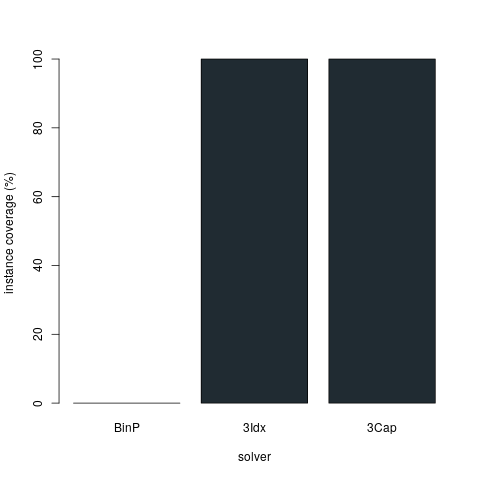
\includegraphics[width=1.2\textwidth]{img/solver_instance_coverage_b=3_m_60s.png}
\caption{\textsc{Zeitlimit} $1min$}
\label{fig:instance_coverage_b=3_m_a}
\end{subfigure}
\hfill
\begin{subfigure}[b]{0.3\textwidth}
\centering
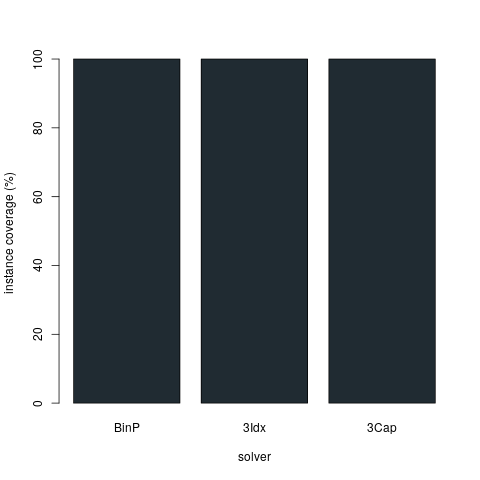
\includegraphics[width=1.2\textwidth]{img/solver_instance_coverage_b=3_m_120s.png}
\caption{\textsc{Zeitlimit} $2min$}
\label{fig:instance_coverage_b=3_m_b}
\end{subfigure}
\hfill
\begin{subfigure}[b]{0.3\textwidth}
\centering
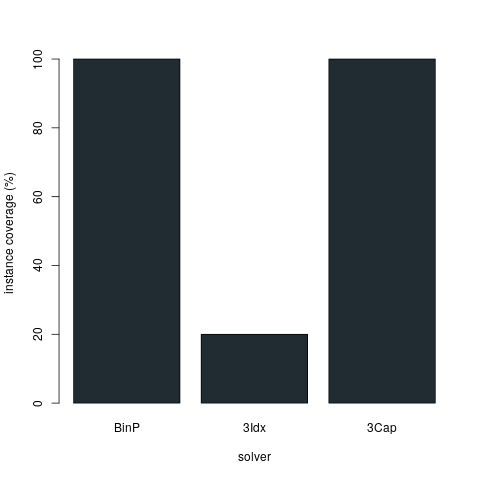
\includegraphics[width=1.2\textwidth]{img/solver_instance_coverage_b=3_m_300s.png}
\caption{\textsc{Zeitlimit} $5min$}
\label{fig:instance_coverage_b=3_m_c}
\end{subfigure}
\caption{\textsc{Instance-Coverage der $b = 3$ Solver (m)}.}
\label{fig:instance_coverage_b=3_m}
\end{figure}

\vfill
\pagebreak

In der Darstellung der Laufzeiten bei einem Zeitlimit von $5$ Minuten in Abb. \ref{fig:b=3_m_runtimes} ist zu sehen, dass die Bin-Packing-Formulierung stets kürzere Laufzeiten besitzt als die 3-Index-Formulierung, welche in $13$ Fällen durch das Zeitlimit gestoppt wird. Ferner ist der Abb. zu entnehmen, dass die Heuristik in Bezug auf die Laufzeit erneut konkurrenzlos ist. Nach durchschnittlich $1.49s$ löst diese sämtliche Instanzen zulässig und unterbietet die MIP-Formulierungen damit erneut sehr deutlich. Aufgrund der Tatsache, dass die Bin-Packing-Formulierung in jedem Fall
vor dem Zeitlimit terminiert, ist außerdem bereits sicher, dass diese sämtliche Instanzen optimal löst.

Für die Kosten gilt, wie man der abermals skalierten Darstellung in Abb. \ref{fig:b=3_m_costs} entnehmen kann, dass die Ergebnisse der Heuristik, wie in vorherigen Experimenten, eine Abweichung von den Optimalwerten der MIP-Formulierungen von durchschnittlich weit unter einem Prozent besitzen. Mit Instanz $01$ gelingt der Heuristik sogar für eine Instanz die
Ermittlung des optimalen Zielfunktionswerts.
Die 3-Index-Formulierung zeigt bei $10$ der $13$ Instanzen, bei welchen diese durch das Zeitlimit
terminiert, erhebliche Abweichungen von den optimalen Zielfunktionswerten und unterliegt in diesen Fällen
deutlich den Lösungen der Heuristik. In den verbleibenden drei Fällen, den Instanzen $00, 07$ und $18$, ermittelt
sie dagegen jeweils den optimalen Zielfunktionswert. Die Stacking-Constraints haben in dieser Kategorie,
basierend auf den in Abb. \ref{fig:b=3_m_costs} dargestellten unteren Schranken, bei jeder Instanz einen Einfluss auf die optimalen Zielfunktionswerte, wenn auch einen sehr geringen.

\begin{figure}[H]
\centering
\begin{subfigure}[b]{0.4\textwidth}
\centering
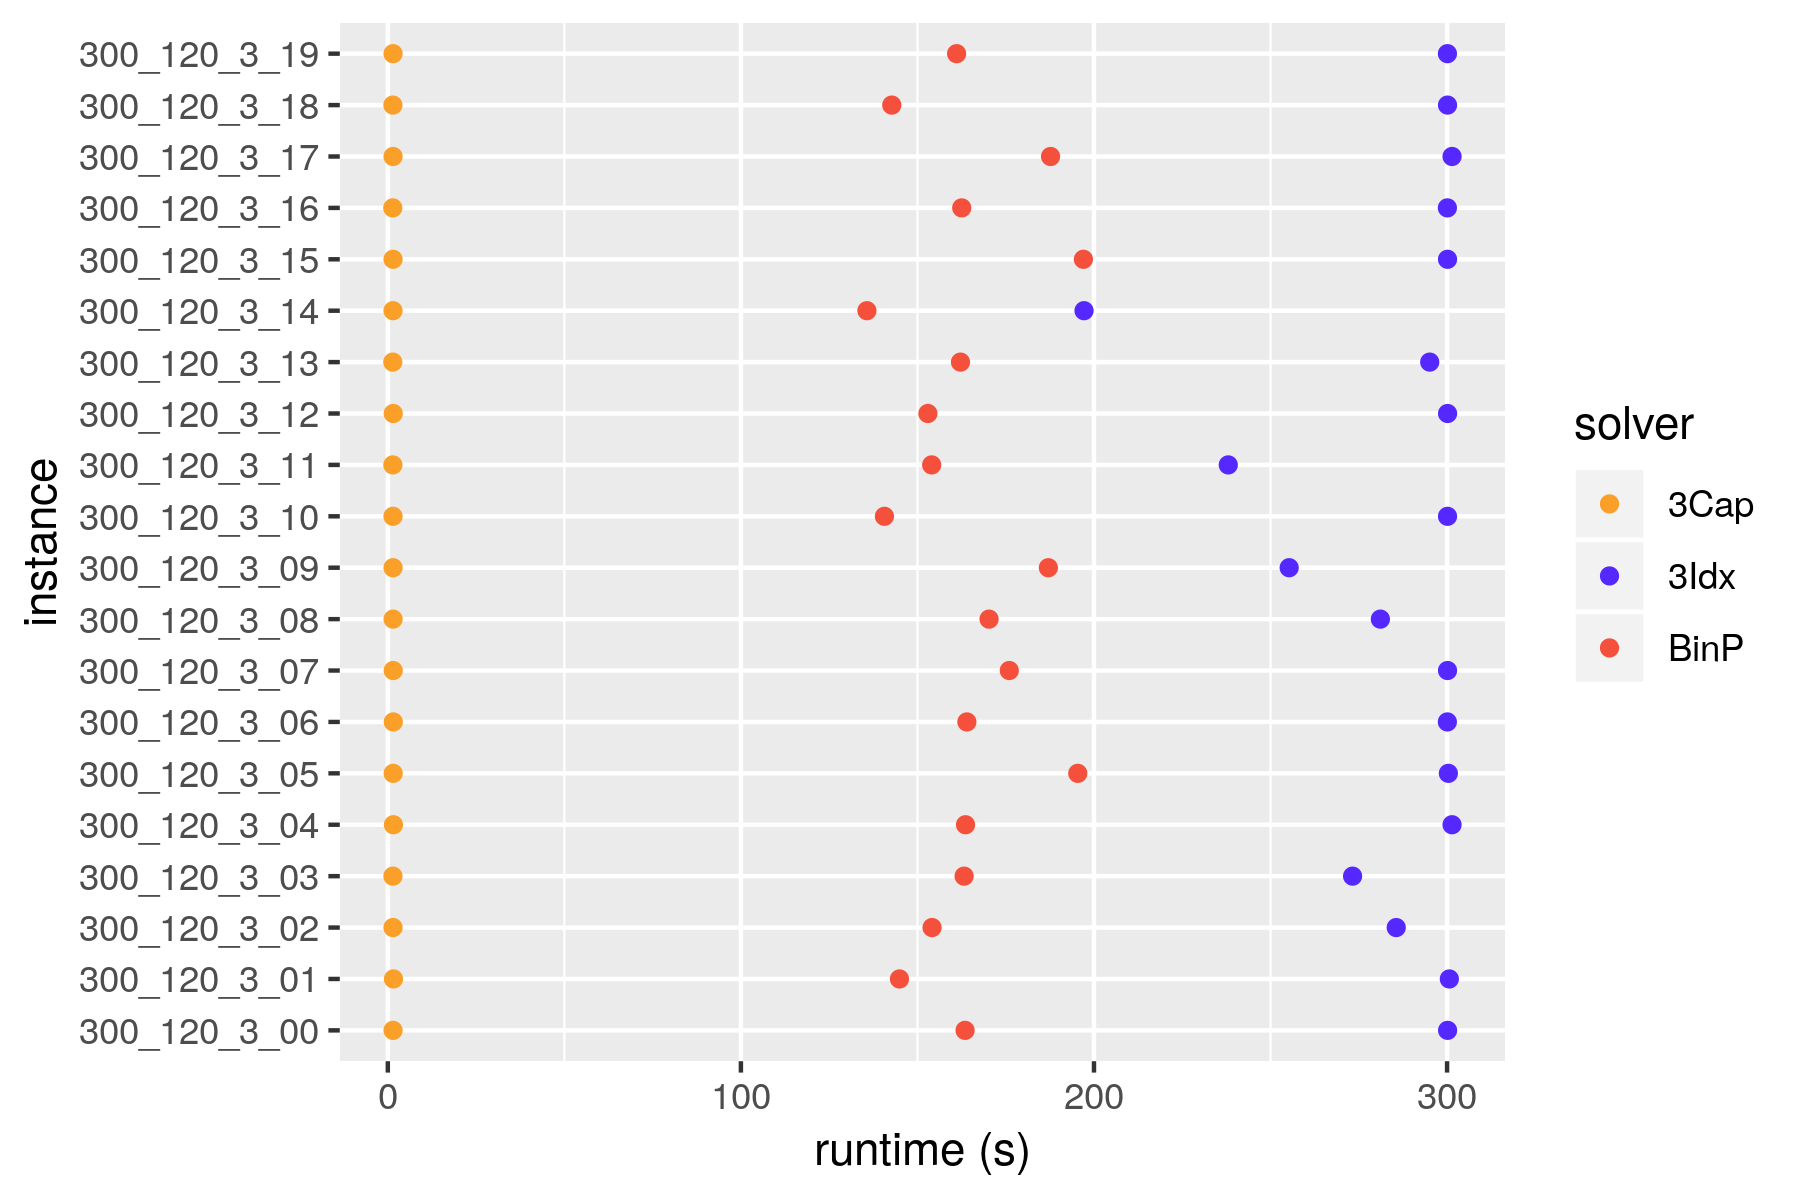
\includegraphics[width=1.3\textwidth]{img/solver_instance_time_b=3_m_300s.png}
\caption{\textsc{Laufzeiten}}
\label{fig:b=3_m_runtimes}
\end{subfigure}
\hfill
\begin{subfigure}[b]{0.4\textwidth}
\centering
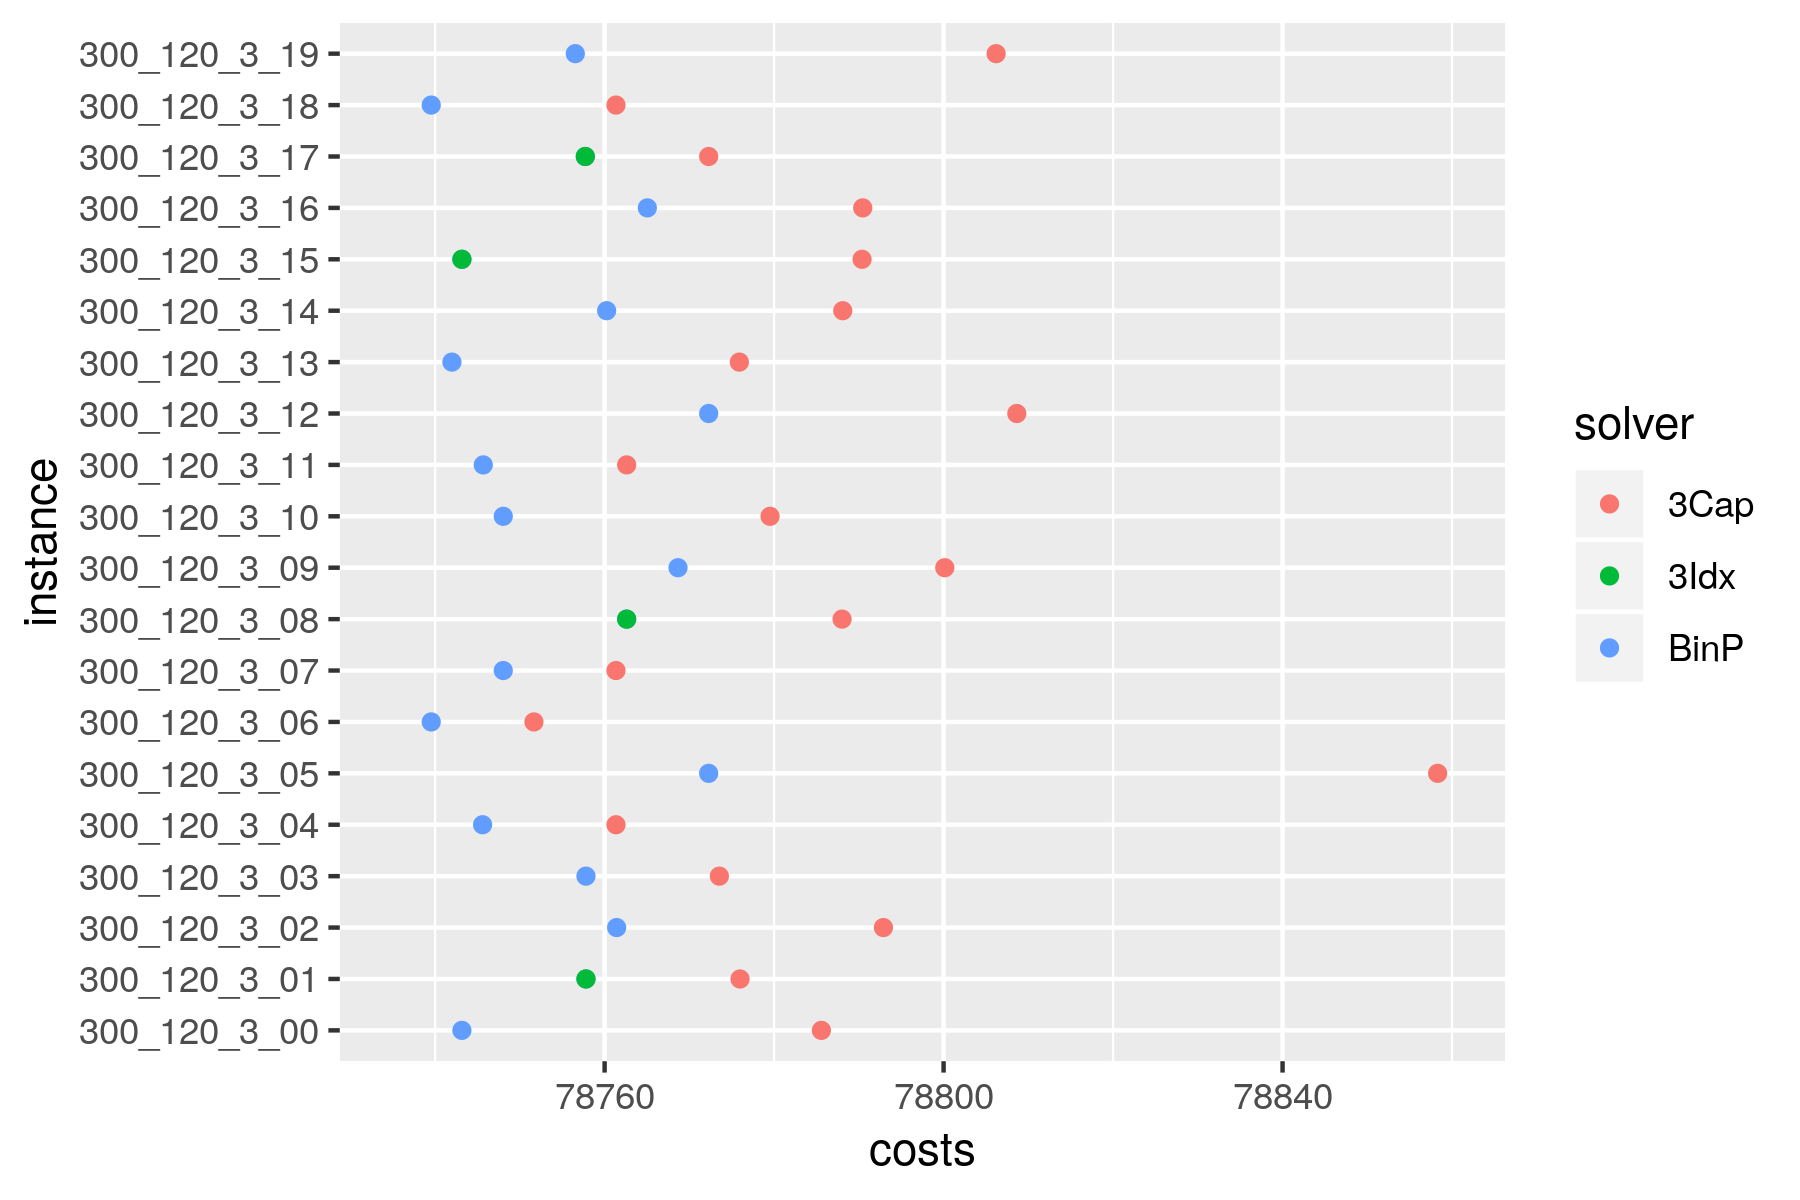
\includegraphics[width=1.3\textwidth]{img/solver_instance_cost_b=3_m_300s.png}
\caption{\textsc{Kosten}}
\label{fig:b=3_m_costs}
\end{subfigure}
\caption{\textsc{Ergebnisse bei $5min$ Zeitlimit}.}
\end{figure}

Wie bereits in der Visualisierung der Instance-Coverage deutlich wurde, löst die Bin-Packing-Formulierung
bei einem Zeitlimit von einer Minute keine Instanz zulässig (vgl. Abb. \ref{fig:mip_results_b=3_m_a}).
Die 3-Index-Formulierung löst dort zwar sämtliche Instanzen zulässig, jedoch keine optimal und weicht
dabei um durchschnittlich $15.01 \%$ vom Optimum ab. Beim betrachteten Zeitlimit von zwei Minuten
löst diese weiterhin keine Instanz optimal und zeigt dieselbe durchschnittliche Abweichung
(vgl. Abb. \ref{fig:mip_results_b=3_m_b}). Die Bin-Packing-Formulierung erreicht bei diesem Zeitlimit zwar ebenfalls
die vollständige Instance-Coverage, löst allerdings trotz der deutlich geringeren durchschnittlichen Abweichung
gleichermaßen keine Instanz optimal. Dies gelingt erst bei einem Zeitlimit von $5$ Minuten, bei welchem die Bin-Packing-Formulierung schließlich mit einer durchschnittlichen Laufzeit von $163.94s$ sämtliche Instanzen optimal löst. Die 3-Index-Formulierung löst hingegen auch bei diesem Zeitlimit lediglich die Hälfte der Instanzen optimal, benötigt dafür durchschnittlich deutlich mehr Zeit und weicht weiterhin um erhebliche $6.62 \%$ vom
Optimum ab (vgl. Abb. \ref{fig:mip_results_b=3_m_c}).

\begin{figure}[H]
\centering
\begin{subfigure}[b]{0.3\textwidth}
\resizebox{\textwidth}{!}{
\begin{tabular}{ | c | c | c |}
    \hline
     & \textbf{BinP} & \textbf{3Idx} \\ \hline
    \textbf{Optimal ($\boldsymbol{\%}$)} & $0$ & $0$ \\ \hline
    \textbf{\O \thinspace Laufzeit ($\boldsymbol{s}$)} & $\textcolor{red}{-}$ & $\textcolor{mygreen}{60.26}$ \\ \hline
    \textbf{\O \thinspace Abweichung ($\boldsymbol{\%}$)} & $\textcolor{red}{-}$ & $\textcolor{mygreen}{15.01}$ \\ \hline
\end{tabular}}
\caption{\textsc{Zeitlimit} $1min$}
\label{fig:mip_results_b=3_m_a}
\end{subfigure}
% $\quad\quad\quad\quad$
\begin{subfigure}[b]{0.3\textwidth}
\resizebox{\textwidth}{!}{
\begin{tabular}{ | c | c | c |}
    \hline
     & \textbf{BinP} & \textbf{3Idx} \\ \hline
    \textbf{Optimal ($\boldsymbol{\%}$)} & $ 0$ & $ 0$ \\ \hline
    \textbf{\O \thinspace Laufzeit ($\boldsymbol{s}$)} & $\textcolor{red}{120.89}$ & $\textcolor{mygreen}{120.17}$ \\ \hline
    \textbf{\O \thinspace Abweichung ($\boldsymbol{\%}$)} & $\textcolor{mygreen}{2.63}$ & $\textcolor{red}{15.01}$ \\ \hline
\end{tabular}}
\caption{\textsc{Zeitlimit} $2min$}
\label{fig:mip_results_b=3_m_b}
\end{subfigure}
% \end{figure}
% \begin{figure}[H]
\begin{subfigure}[b]{0.3\textwidth}
\resizebox{\textwidth}{!}{
\begin{tabular}{ | c | c | c |}
    \hline
     & \textbf{BinP} & \textbf{3Idx} \\ \hline
    \textbf{Optimal ($\boldsymbol{\%}$)} & $ \textcolor{mygreen}{100}$ & $ \textcolor{red}{50}$ \\ \hline
    \textbf{\O \thinspace Laufzeit ($\boldsymbol{s}$)} & $\textcolor{mygreen}{163.94}$ & $\textcolor{red}{286.52}$ \\ \hline
    \textbf{\O \thinspace Abweichung ($\boldsymbol{\%}$)} & $\textcolor{mygreen}{0.0}$ & $\textcolor{red}{6.62}$ \\ \hline
\end{tabular}}
\caption{\textsc{Zeitlimit} $5min$}
\label{fig:mip_results_b=3_m_c}
\end{subfigure}

\caption{\textsc{MIP-Ergebnisse.}}
\label{fig:mip_results_b=3_m}
\end{figure}

Demzufolge ist die Bin-Packing-Formulierung ab einem Zeitlimit von zwei Minuten mit erheblich besseren Ergebnissen der 3-Index-Formulierung auch in dieser Kategorie klar vorzuziehen.
Die Heuristik benötigt durchschnittlich eine Laufzeit von nur $1.49s$ und weicht dabei um durchschnittlich
$0.03 \%$ vom Optimum ab. Wie bereits in der Kategorie der mittelgroßen Instanzen im $b = 2$ Szenario, ist dieser erhebliche Laufzeitunterschied um mehrere Größenordnungen wohl hinreichende Motivation, um diese jeweils zu vernachlässigende Abweichung vom Optimum in Kauf zu nehmen.

\textbf{Große Instanzen (l)}

Zuletzt werden die Solver für in Kapitel \ref{sec:test_data} als groß bezeichnete Instanzen,
bei denen es darum geht, $500$ eintreffende Items in die Storage-Area zu verladen, verglichen.
In dieser Kategorie werden Zeitlimits von $5, 15$ und $30$ Minuten pro Instanz betrachtet.

Die Bin-Packing-Formulierung findet, wie Abb. \ref{fig:instance_coverage_b=3_l_a} zu entnehmen ist,
bei einem Zeitlimit von $5$ Minuten pro Instanz keine zulässige Lösung, während die 3-Index-Formulierung
$85 \%$ der Instanzen zulässig löst. Beim nächsten betrachteten Zeitlimit von $15$ Minuten pro Instanz löst die Bin-Packing-Formulierung dagegen sämtliche Instanzen zulässig, während die 3-Index-Formulierung weiterhin eine Instance-Coverage von $85 \%$ besitzt (vgl. Abb. \ref{fig:instance_coverage_b=3_l_b}). Es ist bemerkenswert, dass die Bin-Packing-Formulierung bei einem Zeitlimit von $5$ Minuten noch keine Instanz zulässig löst und beim Zeitlimit
von $15$ Minuten eine höhere Instance-Coverage als die 3-Index-Formulierung erreicht. Die verbleibenden $15 \%$ der
Instanzen, welche von der 3-Index-Formulierung nicht gelöst werden, erfordern offensichtlich erheblich längere Laufzeiten als die übrigen. In Abb. \ref{fig:instance_coverage_b=3_l_c} ist die Instance-Coverage bei einem Zeitlimit von $30$ Minuten dargestellt, bei welchem schließlich sämtliche Solver alle betrachteten Instanzen zulässig lösen. Die Heuristik ist mit einer durchschnittlichen Laufzeit von $6.72s$ pro Instanz erneut in keinem Fall vom Zeitlimit betroffen.

\vfill
\pagebreak

\begin{figure}[H]
\centering

\begin{subfigure}[b]{0.3\textwidth}
\centering
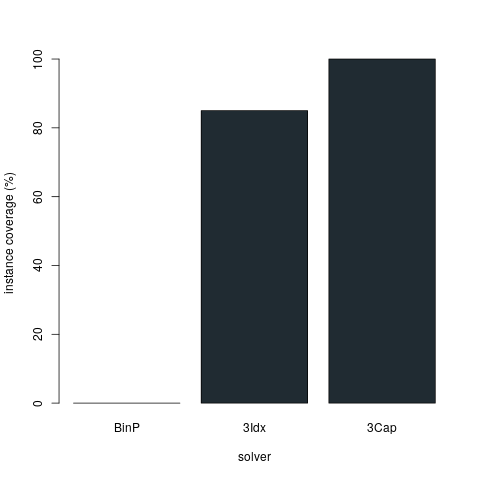
\includegraphics[width=1.2\textwidth]{img/solver_instance_coverage_b=3_l_300s.png}
\caption{\textsc{Zeitlimit} $5min$}
\label{fig:instance_coverage_b=3_l_a}
\end{subfigure}
\hfill
\begin{subfigure}[b]{0.3\textwidth}
\centering
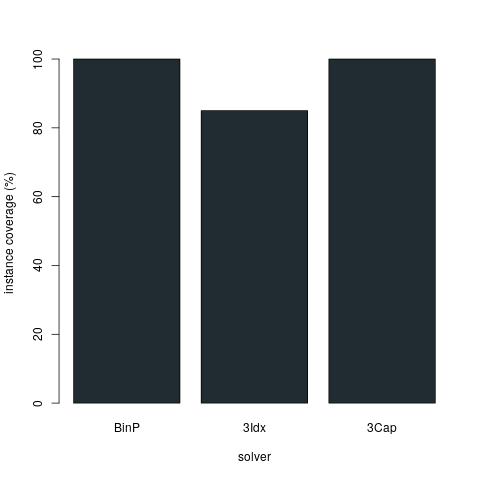
\includegraphics[width=1.2\textwidth]{img/solver_instance_coverage_b=3_l_900s.png}
\caption{\textsc{Zeitlimit} $15min$}
\label{fig:instance_coverage_b=3_l_b}
\end{subfigure}
\hfill
\begin{subfigure}[b]{0.3\textwidth}
\centering
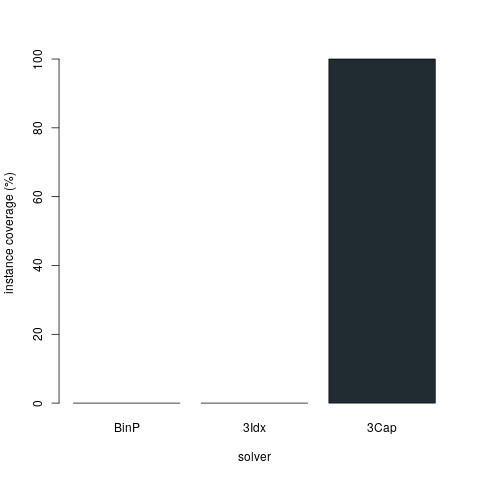
\includegraphics[width=1.2\textwidth]{img/solver_instance_coverage_b=3_l_1800s.png}
\caption{\textsc{Zeitlimit} $30min$}
\label{fig:instance_coverage_b=3_l_c}
\end{subfigure}
\caption{\textsc{Instance-Coverage der $b = 3$ Solver (l)}.}
\label{}
\end{figure}

Wie der Darstellung der Laufzeiten bei einem Zeitlimit von $30$ Minuten in Abb. \ref{fig:b=3_l_runtimes} zu
entnehmen ist, terminiert die Bin-Packing-Formulierung mit Ausnahme von Instanz $06$ stets vor dem Zeitlimit.
Demgegenüber wird die 3-Index-Formulierung ausnahmslos durch das Zeitlimit gestoppt.
Des Weiteren ist klar zu erkennen, dass die Heuristik auch in dieser Kategorie in Bezug auf die Laufzeit konkurrenzlos ist. Da die Bin-Packing-Formulierung bei Instanz $06$ durch das Zeitlimit terminiert, ist in diesem Fall nicht garantiert, dass diese zu einer optimalen Lösung gelangt. In einem weiteren Test mit einem größeren Zeitlimit hat sich allerdings herausgestellt, dass auch dort der Optimalwert ermittelt wurde, was bedeutet, dass
\textsc{CPLEX} lediglich noch nicht bewiesen hat, dass es sich um das Optimum handelt, der entsprechende Wert wurde jedoch bereits ermittelt.

In der abermals skalierten Darstellung der Kosten bei einem Zeitlimit von $30$ Minuten in Abb. \ref{fig:b=3_l_costs}
ist zu erkennen, dass die 3-Index-Formulierung in keinem Fall eine optimale Lösung liefert,
stattdessen kann diese aufgrund der erheblichen Abweichungen vom Optimum in keinem Fall mit den Ergebnissen der Heuristik
oder der Bin-Packing-Formulierung konkurrieren. Außerdem ist zu sehen, dass die Abweichungen der Zielfunktionswerte der Heuristik von jenen der Bin-Packing-Formulierung auch in dieser Kategorie nur sehr gering sind.
Insbesondere bei den Instanzen $06, 10$ und $11$ wurde annähernd der optimale Zielfunktionswert ermittelt.
Die Einträge der unteren Schranken zeigen, dass die Stacking-Constraints erneut bei jeder Instanz einen geringen Einfluss auf den optimalen Zielfunktionswert haben.

\vfill
\pagebreak

\begin{figure}[H]
\centering
\begin{subfigure}[b]{0.4\textwidth}
\centering
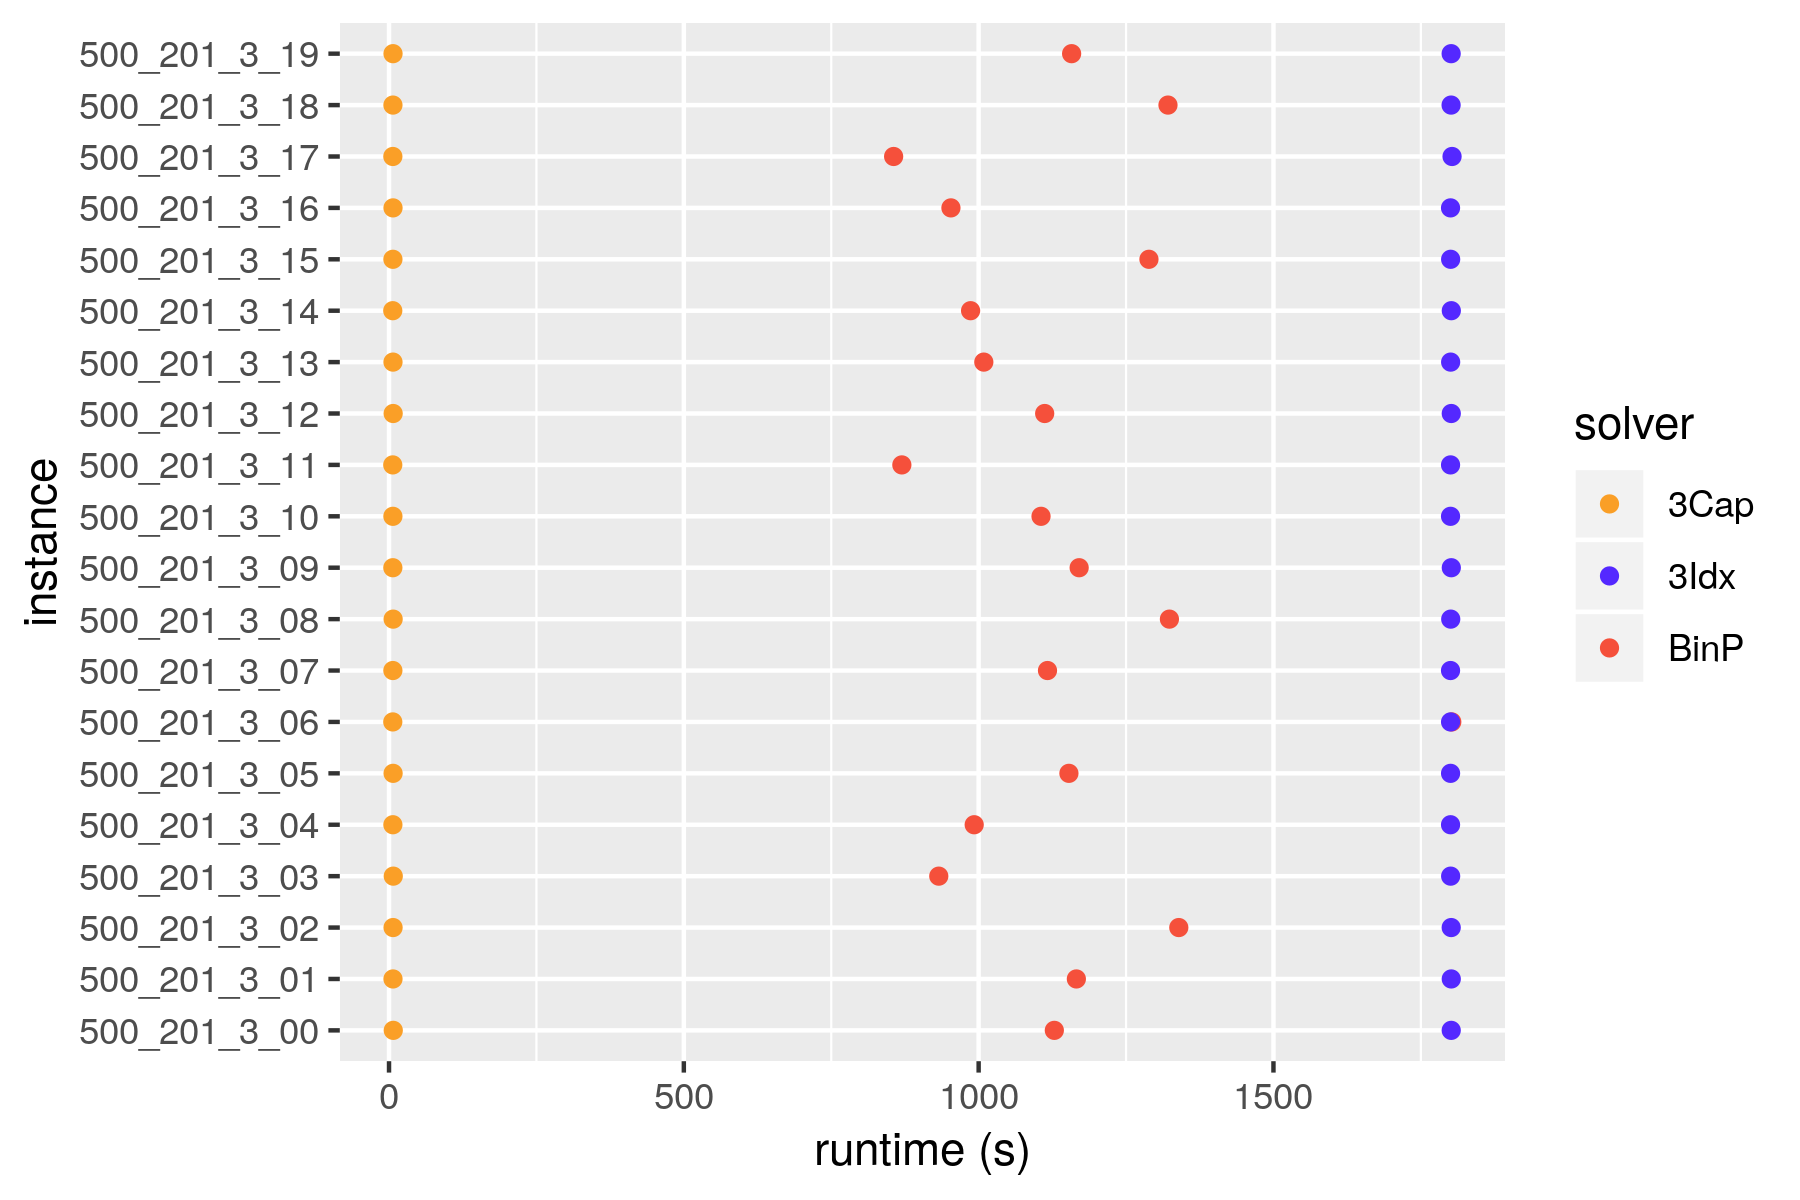
\includegraphics[width=1.3\textwidth]{img/solver_instance_time_b=3_l_1800s.png}
\caption{\textsc{Laufzeiten}}
\label{fig:b=3_l_runtimes}
\end{subfigure}
\hfill
\begin{subfigure}[b]{0.4\textwidth}
\centering
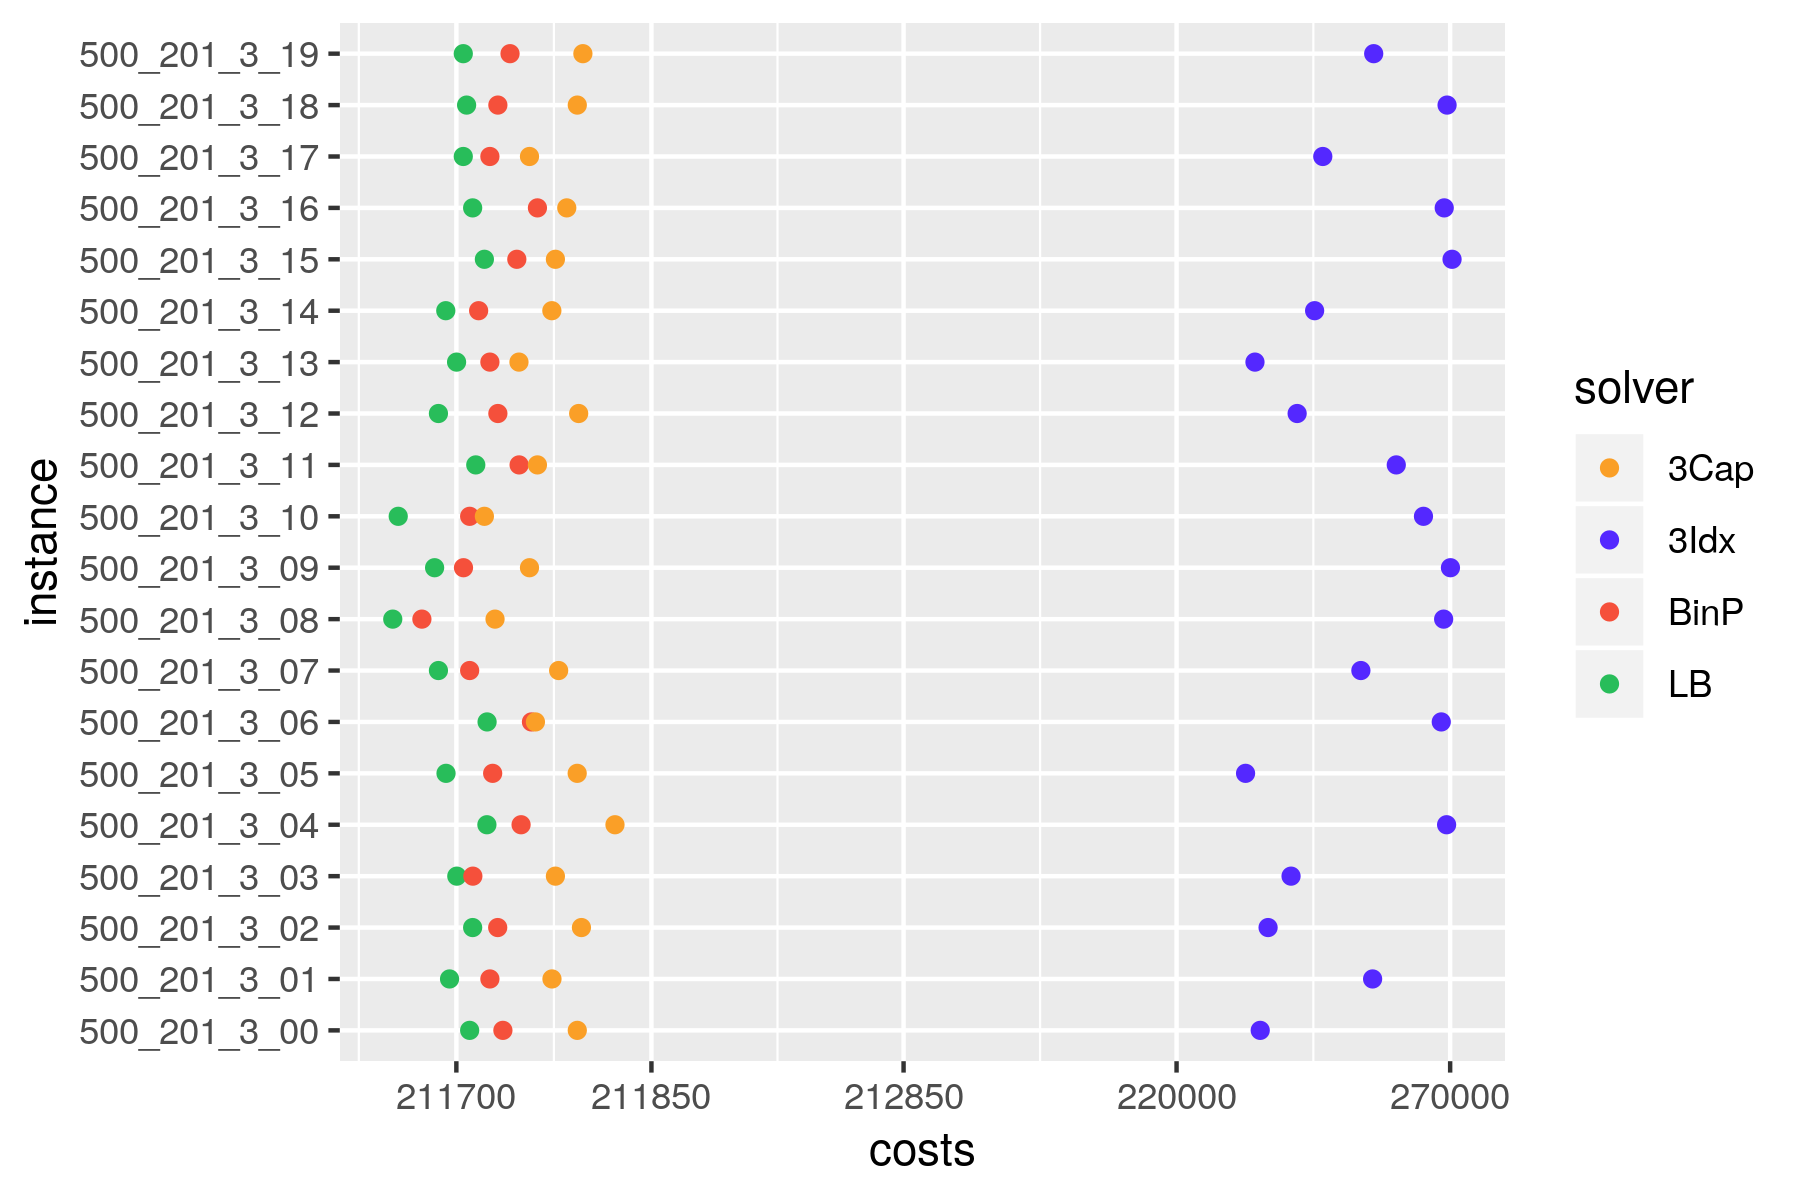
\includegraphics[width=1.3\textwidth]{img/solver_instance_cost_b=3_l_1800s.png}
\caption{\textsc{Kosten}}
\label{fig:b=3_l_costs}
\end{subfigure}
\caption{\textsc{Ergebnisse bei $30min$ Zeitlimit}.}
\label{fig:res_plots_b=3_l}
\end{figure}

Wie bereits anhand der ermittelten Zielfunktionswerte beim größten betrachteten Zeitlimit deutlich wurde,
ist die 3-Index-Formulierung in dieser Kategorie erneut der Bin-Packing-Formulierung unterlegen,
welche, wie in Abb. \ref{fig:mip_results_b=3_l_c} nachzuvollziehen ist, nach durchschnittlich etwa $19$ Minuten sämtliche Instanzen optimal löst. Dies gilt allerdings erst ab dem betrachteten Zeitlimit
von $15$ Minuten. Beim Zeitlimit von $5$ Minuten gelangt, wie man den Abbildungen \ref{fig:instance_coverage_b=3_l_a} und \ref{fig:mip_results_b=3_l_a} entnehmen kann, die 3-Index-Formulierung zu besseren Ergebnissen.
Es sollte allerdings berücksichtigt werden, dass auch die Bin-Packing-Formulierung bei einem Zeitlimit von
$15$ Minuten noch derart große Abweichungen von den optimalen Zielfunktionswerten zeigt, dass diese
praktisch erst ab dem betrachteten Zeitlimit von $30$ Minuten sinnvoll einsetzbar ist.
Die Heuristik löst mit einer durchschnittlichen Laufzeit von $6.72s$ pro Instanz sämtliche Instanzen
zulässig und weicht dabei im Durchschnitt nur um $0.02 \%$ vom Optimum ab.

\begin{figure}[H]
\begin{subfigure}[b]{0.3\textwidth}
\centering
\resizebox{\textwidth}{!}{
\begin{tabular}{ | c | c | c |}
    \hline
     & \textbf{BinP} & \textbf{3Idx} \\ \hline
    \textbf{Optimal ($\boldsymbol{\%}$)} & $0$ & $0$ \\ \hline
    \textbf{\O \thinspace Laufzeit ($\boldsymbol{s}$)} & $\textcolor{red}{-}$ & $\textcolor{mygreen}{301.17}$ \\ \hline
    \textbf{\O \thinspace Abweichung ($\boldsymbol{\%}$)} & $\textcolor{red}{-}$ & $\textcolor{mygreen}{15.43}$ \\ \hline
\end{tabular}}
\caption{\textsc{Zeitlimit} $5min$}
\label{fig:mip_results_b=3_l_a}
\end{subfigure}
% $\quad\quad\quad\quad$
\begin{subfigure}[b]{0.3\textwidth}
\centering
\resizebox{\textwidth}{!}{
\begin{tabular}{ | c | c | c |}
    \hline
     & \textbf{BinP} & \textbf{3Idx} \\ \hline
    \textbf{Optimal ($\boldsymbol{\%}$)} & $ \textcolor{mygreen}{20}$ & $ \textcolor{red}{0}$ \\ \hline
    \textbf{\O \thinspace Laufzeit ($\boldsymbol{s}$)} & $\textcolor{red}{901.50}$ & $\textcolor{mygreen}{900.74}$ \\ \hline
    \textbf{\O \thinspace Abweichung ($\boldsymbol{\%}$)} & $\textcolor{mygreen}{6.30}$ &$\textcolor{red}{15.43}$ \\ \hline
\end{tabular}}
\caption{\textsc{Zeitlimit} $15min$}
\label{fig:mip_results_b=3_l_b}
\end{subfigure}
% \end{figure}
% \begin{figure}[H]
\begin{subfigure}[b]{0.3\textwidth}
\centering
\resizebox{\textwidth}{!}{
\begin{tabular}{ | c | c | c |}
    \hline
     & \textbf{BinP} & \textbf{3Idx} \\ \hline
    \textbf{Optimal ($\boldsymbol{\%}$)} & $ \textcolor{mygreen}{100}$ & $ \textcolor{red}{0}$ \\ \hline
    \textbf{\O \thinspace Laufzeit ($\boldsymbol{s}$)} & $\textcolor{mygreen}{1139.19}$ & $\textcolor{red}{1800.98}$ \\ \hline
    \textbf{\O \thinspace Abweichung ($\boldsymbol{\%}$)} & $\textcolor{mygreen}{0.0}$ &$\textcolor{red}{17.17}$ \\ \hline
\end{tabular}}
\caption{\textsc{Zeitlimit} $30min$}
\label{fig:mip_results_b=3_l_c}
\end{subfigure}
\caption{\textsc{MIP-Ergebnisse.}}
\label{}
\end{figure}

Zur Verdeutlichung der Tatsache, dass die konstruktiven Heuristiken in der Lage sind, auch erheblich
größere Instanzen effizient zu lösen, wurden $20$ Instanzen generiert, bei denen es darum geht,
$1000$ Items in die Storage-Area zu verladen. Instanzen dieser Größe können nicht mehr effizient
von den MIP-Formulierungen gelöst werden, weshalb sie gut geeignet sind, um die Stärke der Heuristiken
zu demonstrieren. In Abb. \ref{fig:big_instance_example} sind die ermittelten Zielfunktionswerte dargestellt.
Als Referenzwerte dienen jeweils die unteren Schranken, welche zeigen, dass die Heuristik auch bei Instanzen dieser
Größe nur marginal von den Optimalwerten abweicht. Die durchschnittlich benötigte Laufzeit pro Instanz beträgt
dabei lediglich $56.73s$.

\vfill
\pagebreak

\begin{figure}[H]
\centering

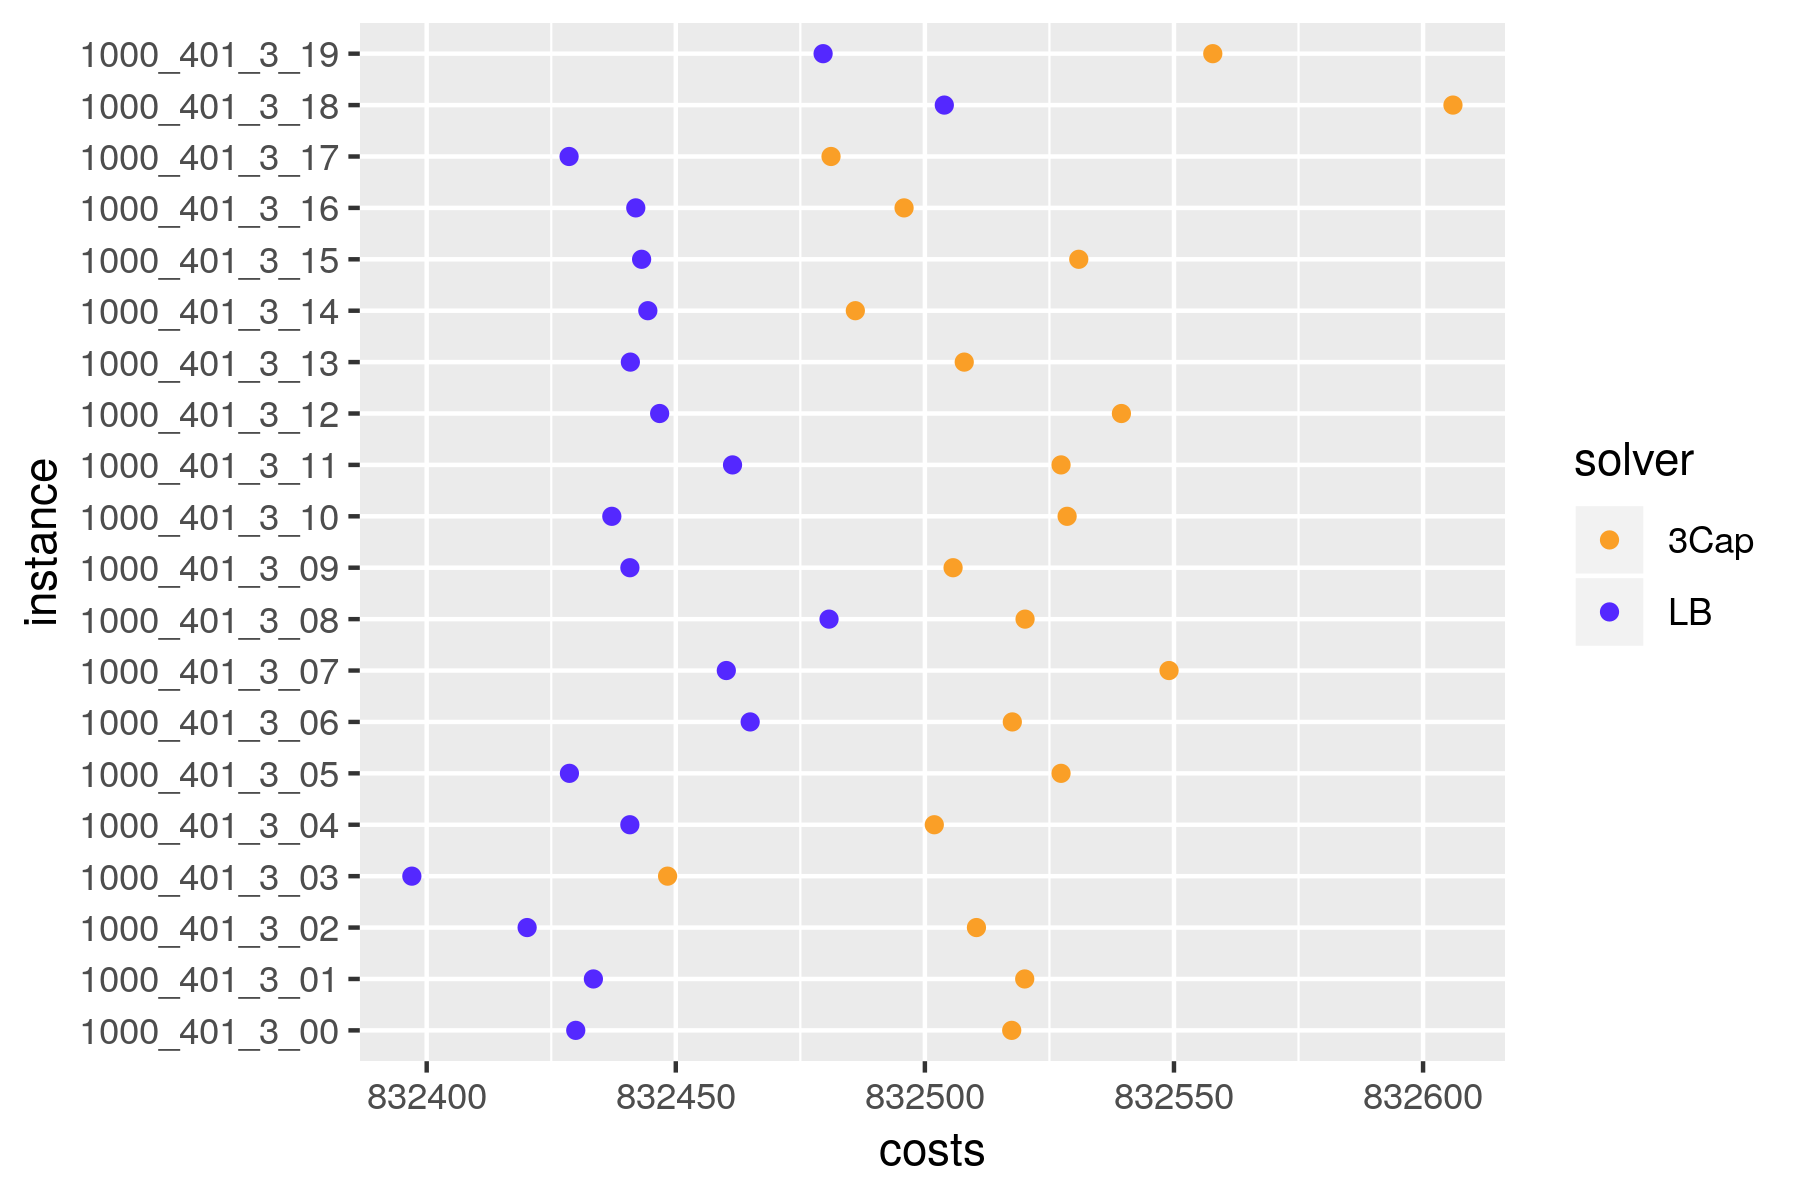
\includegraphics[width=0.6\textwidth]{img/big_instance_example.png}
\caption{\textsc{Zielfunktionswerte der 3Cap-Heuristik}.}
\label{fig:big_instance_example}

\end{figure}

\textbf{Fazit}\newline

Bei Stacking-Problemen mit Stacks der Kapazität $b = 3$ besteht in der Kategorie der kleinen Instanzen
aufgrund der relativ geringen Laufzeit der Bin-Packing-Formulierung nicht zwingend ein Bedarf für eine
Laufzeitverbesserung durch eine Heuristik. Nichtsdestotrotz ist die Heuristik bei einer nur geringen
durchschnittlichen Abweichung vom Optimum noch einmal erheblich schneller als diese.
In der Kategorie der mittelgroßen Instanzen ist die Bin-Packing-Formulierung der 3-Index-Formulierung sogar
sehr deutlich vorzuziehen. Da jedoch auch die Bin-Packing-Formulierung durschnittlich fast $3$ Minuten zur exakten Lösung benötigt, ermöglicht die Heuristik hier mit einer durchschnittlichen Laufzeit von nur $1.5$ Sekunden eine derart große Laufzeitersparnis, dass die sehr geringe Abweichung von $0.03 \%$ in Kauf genommen werden sollte.
Noch deutlicher äußert sich dieser Trend in der Kategorie der großen Instanzen, in welcher die 3-Index-Formulierung
selbst bei einem Zeitlimit von $30$ Minuten keine Instanz optimal löst. Die Bin-Packing-Formulierung, welche dort
mit einer durchschnittlichen Laufzeit von etwa $19$ Minuten sämtliche Instanzen optimal löst,
ist demnach bei einer Stack-Kapazität von $b = 3$ in jeder Kategorie der 3-Index-Formulierung vorzuziehen.
Die Heuristik benötigt hier durschnittlich $6.72s$ pro Instanz und weicht um durchschnittlich $0.02 \%$ vom Optimum ab.
Der daraus resultierende noch gravierendere Unterschied der Laufzeiten zwischen der Bin-Packing-Formulierung und
der Heuristik sorgt in Verbindung mit der sehr geringen Abweichung vom Optimum dafür, dass die Heuristik in der Praxis
auch in dieser Kategorie bevorzugt werden sollte.

Insgesamt ist festzuhalten, dass die Heuristik in jeder betrachteten Kategorie bei sehr geringen Abweichungen
vom Optimum deutlich kürzere Laufzeiten als die von \textsc{CPLEX} gelösten MIP-Formulierungen bietet und somit in
jedem Fall eine gute Alternative darstellt. Je größer die Instanzen werden, desto besser schneidet die Heuristik
verglichen mit den MIP-Formulierungen ab und sollte bereits ab der Kategorie der mittelgroßen Instanzen in der Regel
den MIP-Formulierungen vorgezogen werden.

\vfill
\pagebreak

\section{Verbesserungsverfahren}
\label{sec:post_optimization}

Bei Verbesserungsverfahren handelt es sich um lokale Suchverfahren, welche bereits mit einer Lösung des Problems starten, die z.B. durch ein konstruktives Eröffnungsverfahren, wie die Heuristiken aus den Kapiteln \ref{sec:two_cap_heuristic} und \ref{sec:three_cap_heuristic}, bestimmt wurde und versuchen diese im Laufe des Verfahrens zu verbessern. Dabei wird zwischen deterministischen Verfahren, die bei gleichen Startlösungen und gleichen Rahmenbedingungen stets zum gleichen Ergebnis kommen und stochastischen Verfahren, bei denen durch den Einsatz einer Zufallskomponente unterschiedliche Lösungen generiert werden, unterschieden \cite{Knust2017}.

Zunächst werden in Abschnitt \ref{sec:local_search} die Grundlagen zu lokalen Suchverfahren eingeführt.
Anschließend geht es in Abschnitt \ref{sec:tabu_search} um das allgemeine Verfahren einer Tabu-Suche,
bevor in Abschnitt \ref{sec:tabu_search_for_sp} konkret die entwickelte Tabu-Suche zur Lösung von Stacking-Problemen
beschrieben wird. Letztlich wird in Abschnitt \ref{sec:tabu_search_config} die Konfiguration der Tabu-Suche erläutert,
die den Ergebnissen der Anwendung dieser, welche in Abschnitt \ref{sec:tabu_search_experiments} präsentiert werden,
zugrunde liegt.

\subsection{Lokale Suchverfahren}
\label{sec:local_search}

Beim in dieser Arbeit betrachteten lokalen Suchverfahren handelt es sich um eine sogenannte Metaheuristik,
weil dieses nicht auf ein spezielles Problem abzielt, sondern auf grundsätzlichen Suchprinzipien beruht,
die auf eine Vielzahl von Optimierungsproblemen anwendbar sind. Aus diesem Grund erfreuen sich diese Heuristiken einer sehr großen Beliebtheit, sie sind allgemein anwendbar und sehr flexibel an konkrete Problemstellungen anpassbar.
Eine lokale Suche ist ein iterativer Prozess, bei welchem von einer Lösung zur nächsten, verbessernden Lösung vorangeschritten wird, bis ein bestimmtes Abbruchkriterium erfüllt ist. Um den Lösungsraum systematisch zu durchsuchen, wird die
sogenannte Nachbarschaft einer Lösung definiert, die der Menge der Lösungen entspricht, welche im nächsten Schritt
von der gegenwärtigen Lösung erreichbar sind \cite{Brucker2006}.
Die Idee eines lokalen Suchverfahrens ist es also, ausgehend von einer Initiallösung durch wohldefinierte Regeln zu anderen,
verbessernden Lösungen innerhalb der Nachbarschaft zu gelangen. Dabei wird häufig solange fortgeschritten, bis keine verbessernde Lösung in der Nachbarschaft gefunden wird, also bis ein lokales Minimum erreicht ist.
Der Erfolg dieses Ansatzes und somit die Lösungsqualität hängt primär von der definierten Struktur
der Nachbarschaft ab \cite{Pirlot1996}.
Die größte Schwäche dieses Ansatzes ist die Unfähigkeit, lokale Minima zu verlassen. Dieses Problem ist sehr
anschaulich in Abb. \ref{fig:local_search_weakness} visualisiert. Darin sind sämtliche Lösungen in der
Nachbarschaft $V(x_n)$ schlechter als die gegenwärtige Lösung $x_n$, obwohl weiter entfernt ein globales Minimum
existiert, welches aufgrund der Tatsache, dass ausschließlich verbessernde Lösungen gewählt werden,
nicht erreicht werden kann.

\vfill
\pagebreak

\begin{figure}[H]
\centering
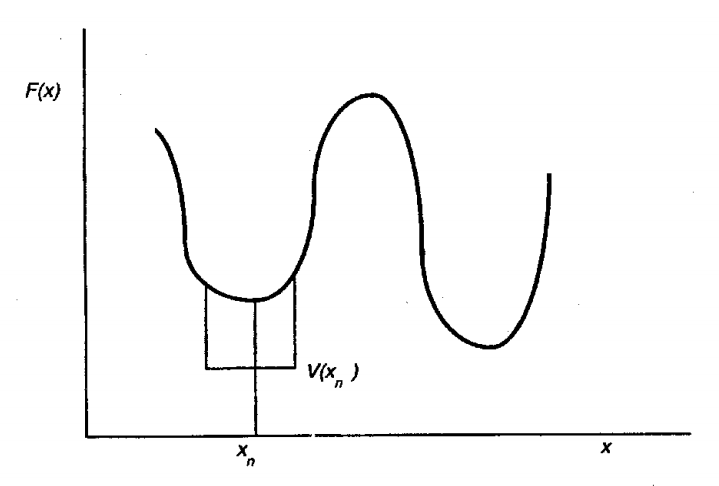
\includegraphics[width=0.5\textwidth]{img/local_minimum.png}
\caption{\textsc{Schwäche lokaler Suchverfahren \cite{Pirlot1996}.}}
\label{fig:local_search_weakness}
\end{figure}

\textbf{Formaler Ablauf einer lokalen Suche}

Eine lokale Suche startet mit einer beliebigen Lösung $x_1 \in X$ und in jedem Schritt $n$
wird eine neue Lösung $x_{n+1}$ aus der Nachbarschaft $V(x_n)$ der gegenwärtigen Lösung $x_n$ gewählt.
Für jedes $x \in X$ existiert eine solche Nachbarschaft $V(x) \subseteq X$.
Typischerweise entspricht das Kriterium, anhand welchem die nächste Lösung $x_{n+1}$ gewählt wird,
die beste Lösung in der Nachbarschaft von $x_n$ zu wählen, also eine Lösung $x_{n+1} \in V(x_n)$
mit $F(x_{n+1}) \leq F(x) \thinspace \forall \thinspace x \in V(x_n)$ bei Betrachtung eines
Minimierungsproblems \cite{Pirlot1996}.

Sollte keine verbessernde Lösung in der Nachbarschaft gefunden werden, so terminiert die Suche.
Diese Strategie wird \textquote{Steepest Descent} genannt, also Strategie des steilsten Abstiegs.
Dieser Name ergibt sich daraus, dass bei einem Minimierungsproblem in der Richtung des steilsten Abstiegs
von der Initiallösung vorangeschritten wird, bis keine Verbesserung mehr erzielt wird,
was zum bereits erwähnten Problem aus Abb. \ref{fig:local_search_weakness} führt.

\textbf{Beispiel}

Ein simples Beispiel für eine solche Nachbarschaft lässt sich anhand eines Bitvektors demonstrieren.
Wenn $X$ eine Menge von Bitvektoren ist und $x \in X$, dann kann eine Nachbarschaft $V(x)$ als die Menge
sämtlicher Lösungen $x \in X$ definiert werden, bei denen in $x$ ein einzelnes Bit invertiert wird \cite{Pirlot1996}.

Sei $x = (1, 0, 1, 0, 1, 0)$ eine als Bitvektor kodierte Lösung.
Die Nachbarschaft dieser Lösung ergibt sich gemäß der beschriebenen Struktur wie folgt:
\[
V(x) =
  \begin{bmatrix}
    \boldsymbol{0} & 0 & 1 & 0 & 1 & 0 \\
    1 & \boldsymbol{1} & 1 & 0 & 1 & 0 \\
    1 & 0 & \boldsymbol{0} & 0 & 1 & 0 \\
    1 & 0 & 1 & \boldsymbol{1} & 1 & 0 \\
    1 & 0 & 1 & 0 & \boldsymbol{0} & 0 \\
    1 & 0 & 1 & 0 & 1 & \boldsymbol{1}
  \end{bmatrix}
\]

\vfill
\pagebreak

\subsection{Tabu-Suche}
\label{sec:tabu_search}

Die größte Schwäche des in Kapitel \ref{sec:local_search} vorgestellten allgemeinen lokalen Suchverfahrens
ist, dass die generierte Lösung nur einem lokalen Optimum entspricht und daher möglicherweise stark vom globalen
Optimum abweicht. Eine gute Qualität der Lösung ist somit nicht garantiert.
Eine Strategie um diesem Problem entgegenzutreten wäre beispielsweise, das Verfahren mehrfach mit unterschiedlichen
Initiallösungen zu starten und anschließend das beste generierte lokale Optimum zu wählen.
Ein weiterer Ansatz ist, Verschlechterungen des Zielfunktionswerts während des Suchprozesses zu erlauben.
Dies führt allerdings dazu, dass Lösungen mehrfach besucht werden können und somit Zyklen entstehen.
Daher müssen in solchen Ansätzen zusätzliche Strategien umgesetzt werden, die Zyklen vermeiden \cite{Brucker2006}.
Genau dort setzt das Verfahren der sogenannten Tabu-Suche an, welches zum Ziel hat, Situationen, wie jene aus
Abb. \ref{fig:local_search_weakness}, zu vermeiden.

Die Strategie, mit welcher lokale Optima verlassen werden können, ist die folgende.
Sogar wenn in der Nachbarschaft $V(x_n)$ keine bessere Lösung als die gegenwärtige Lösung $x_n$ existiert,
wird zur besten Lösung $x \in V(x_n)$ vorangeschritten.
Da die gesamte Nachbarschaft zu groß sein kann, um diese effizient zu durchsuchen,
wird dabei häufig nur ein Teil der Nachbarschaft $V'(x_n) \subseteq V(x_n)$ betrachtet \cite{Pirlot1996}.
Dieses Vorgehen führt dazu, dass es zu Zyklen kommen kann. Entspricht die gegenwärtige Lösung $x$,
so wird anschließend die beste Lösung $x_n \in V(x)$ gewählt. Daraufhin besteht die Chance,
dass die beste Lösung in $V(x_n)$ erneut $x$ ist. D.h. es entsteht ein Zyklus, in welchem wiederkehrend
zwischen den Lösungen $x$ und $x_n$ gewechselt wird.
Unter anderem zur Vermeidung solcher Situationen, wird eine der Tabu-Suche ihren Namen gebende Tabu-Liste verwendet,
welche bereits besuchte Lösungen speichert. Ist eine Lösung $x$ Teil der Tabu-Liste, so ist der Übergang
von $x_n$ zu $x$ verboten bzw. \textquote{tabu}.
In der Regel werden in der Tabu-Liste aus Effizienzgründen jedoch nicht vollständige Lösungen gespeichert, sondern
bestimmte Attribute der Lösungen oder auch die Operation, welche durchgeführt wurde, um zur jeweiligen Lösung zu gelangen. Im Fall des Bitvektor-Beispiels wäre es z.B. die Information, dass Bit $i$ von $0$ auf $1$ gesetzt wurde.
Die primäre Funktion der Tabu-Liste besteht allerdings darin, die Suche zu diversifizieren,
indem in zuvor undurchsuchten Regionen des \textquote{Search Space}\footnote{Menge, welche nach den zu findenden Objekten durchsucht werden soll.} gesucht wird und lokale Optima verlassen werden \cite{Pirlot1996}.

Der allgemeine Ablauf einer Tabu-Suche ist in Abb. \ref{fig:tabu_search_algo}
dargestellt. Zunächst wird eine initiale Lösung $s$ aus der Menge der zulässigen Lösungen $S$ generiert.
Anschließend wird die beste Lösung $s^*$ mit der Lösung $s$ initialisiert, ebenso wie der beste Zielfunktionswert
$c^*$, welcher mit dem Zielfunktionswert von $s$ initialisiert wird. Außerdem wird eine leere Tabu-Liste $TL$
angelegt. Daraufhin wird in einer Schleife jeweils die Nachbarschaft der gegenwärtigen Lösung $s$ durchsucht. Dazu wird eine
Kandidatenmenge $Cand(s)$ der Lösung $s$ generiert, bei welcher es sich um eine Teilmenge der Nachbarschaft von $s$
handelt, wobei eine zu $s$ benachbarte Lösung nur dann akzeptiert wird, wenn diese nicht Teil der Tabu-Liste ist,
oder diese ein Aspirationskriterium\footnote{Kriterium, welches bei Erfüllung zur Missachtung des Tabu-Status führt.} erfüllt. Aus dieser wird anhand einer Selektionsstrategie eine Nachbarlösung $s'$ gewählt und die Tabu-Liste wird aktualisiert, sodass sämtliche Lösungen, welche besucht werden, als zukünftig \textquote{tabu} gespeichert werden. In jeder Iteration wird die gegenwärtige Lösung $s$ entsprechend durch eine benachbarte Lösung $s'$ aktualisiert.
Sollte $s'$ einen besseren Zielfunktionswert besitzen als $s^*$, so wird die beste Lösung $s^*$
sowie der beste Zielfunktionswert $c^*$ aktualisiert. Dieser Prozess terminiert, sobald ein definiertes
Abbruchkriterium erfüllt ist.

\begin{figure}[H]
\centering
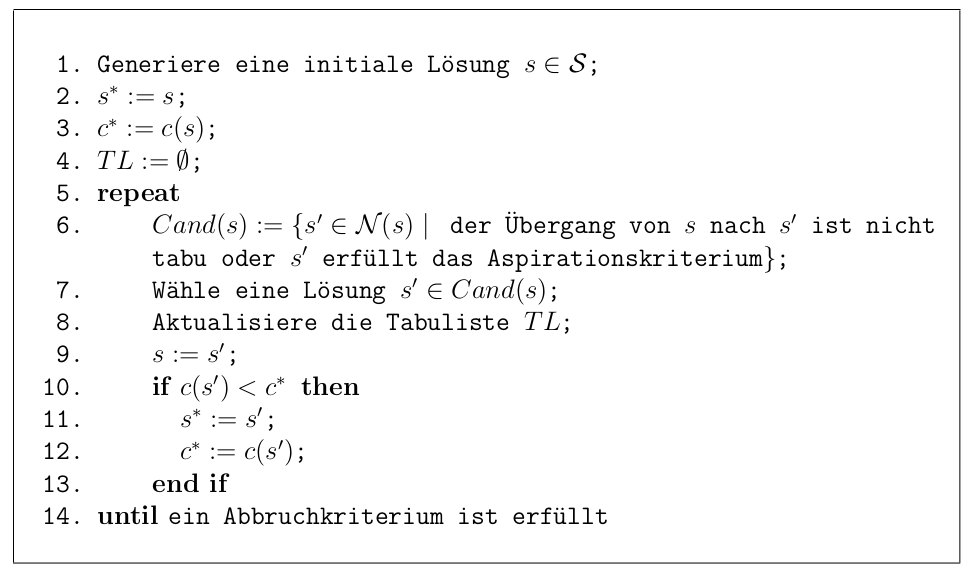
\includegraphics[width=0.9\textwidth]{img/tabu_search_algo_placeholder.png}
\caption{\textsc{Tabu-Suche \cite{Knust2017}.}}
\label{fig:tabu_search_algo}
\end{figure}

Die Qualität der von einer Tabu-Suche generierten Lösungen hängt stark von den vielen
Konfigurations- und Spezifikationsmöglichkeiten ab, welche bei der Entwicklung einer Tabu-Suche gegeben sind.
Die wohl wichtigste Spezifikation ist jene der Nachbarschaftsstruktur. Da in der Regel nicht die vollständige Nachbarschaft einer Lösung besucht wird, wird häufig eine feste Anzahl zufälliger Nachbarn innerhalb der Nachbarschaft besucht. Wie bereits erwähnt, werden zumeist nicht vollständige Lösungen in der Tabu-Liste
gespeichert, weshalb auch die Entscheidung darüber, welche Informationen dort gespeichert werden,
von Relevanz ist. Außerdem wird über ein Aspirationskriterium die Möglichkeit gegeben, dass in bestimmten Fällen
der Tabu-Status einer Lösung bzw. eines Übergangs zu einer anderen Lösung ignoriert wird,
z.B. wenn dieser zu einer bisher besten Lösung führt. Schließlich muss ein sinnvolles
Abbruchkriterium definiert werden, welches die Suche beendet. Im Folgenden wird die in dieser Arbeit entwickelte
Tabu-Suche zur Lösung von Stacking-Problemen vorgestellt.

\vfill
\pagebreak

\subsection{Tabu-Suche zur Lösung von Stacking-Problemen}
\label{sec:tabu_search_for_sp}

Im allgemeinen Tabu-Suche Algorithmus aus Abb. \ref{fig:tabu_search_algo} wird eine initiale Lösung generiert.
Die in dieser Arbeit entwickelte Tabu-Suche generiert die Initiallösung dagegen nicht, sondern bekommt eine
von den konstruktiven Heuristiken aus den Abschnitten \ref{sec:two_cap_heuristic}
und \ref{sec:three_cap_heuristic} generierte Lösung als Eingabe. Bevor die Nachbarschaftsstruktur etc. definiert werden kann, muss zunächst die Repräsentation einer solchen Lösung festgelegt werden, welche genau den Zuweisungen von Item-Tupeln zu Stacks, die von den konstruktiven Heuristiken generiert werden, entspricht. Es handelt sich daher um ein zweidimensionales Array, welches sämtliche Zellen der Storage-Area repräsentiert und entsprechend die zugewiesenen Item-Tupel enthält.\newline
Eine allgemeine Tabu-Suche besteht aus drei Hauptstrategien, welche von ihrem Erfinder \citet{Glover90} als Forbidding-Strategy,
Freeing-Strategy und Short-Term-Strategy bezeichnet werden. Diese werden im Folgenden anhand der in dieser Arbeit entwickelten Tabu-Suche erläutert.

Zunächst zur betrachteten Nachbarschaftsstruktur. Um Nachbarlösungen einer gegebenen Lösung zu generieren,
wird eine kombinierte \textquote{Shift}- und \textquote{Swap}-Nachbarschaft verwendet.
Jedes Item $i \in I$ einer gegebenen Lösung befindet sich in einem Stack $q \in Q$ auf einem Level $l \in \{1, \dotsc, b\}$.
Eine \textquote{Shift}-Operation verschiebt das Item $i$ auf einen Level $l \in \{1, \dotsc, b\}$ in einem
Stack $r \in Q$ mit $r \neq q$. Das Item-Tupel $(i_k, \dotsc, i_1)$, welches sich in Stack $r$ befindet, muss nach der Zuweisung des Items $i$ weiterhin zulässig sein. Dementsprechend muss die Stack-Kapazität durch $k \leq b$ eingehalten werden.
Außerdem müssen sowohl die Stacking-Constraints mit $s_{i_{\lambda + 1}i_\lambda} = 1 \thinspace \forall \thinspace
\lambda = 1, \dotsc, k - 1$, als auch die Placement-Constraints mit $t_{i_\lambda q} = 1 \thinspace \forall
\thinspace i_\lambda$ respektiert werden.
Ein \textquote{Swap} entspricht einer Tausch-Operation zwischen zwei unterschiedlichen Items $i, j \in I$,
d.h. $i \neq j$. Eine solche Tausch-Operation kann auch innerhalb eines Stacks $q \in Q$ stattfinden,
in diesem Fall ist ausgehend von einer zulässigen Lösung bereits sichergestellt, dass beide Items bezüglich der Placement-Constraints mit diesem Stack kompatibel sind und es müssen lediglich im Anschluss die Stacking-Constraints überprüft werden. Im Falle eines Swaps zwischen zwei Items $i, j \in I$, welche sich in unterschiedlichen Stacks $q, r \in Q$ befinden, wobei $i \in q$ und $j \in r$, müssen beide Items in Bezug auf die Placement- und Stacking-Constraints kompatibel zum jeweils anderen Stack sein. Ist dies der Fall, so wird Item $i$ an der Stelle von Item $j$ in Stack $r$ platziert und umgekehrt.

\textbf{Forbidding-Strategy}

Die Forbidding-Strategy spezifiziert die Art der Einträge, also die Art der gespeicherten Information in der
Tabu-Liste. Wie bereits erwähnt, werden aus Effizienzgründen typischerweise nicht die Lösungen selbst gespeichert,
sondern bestimmte Attribute der Lösungen oder Operatoren, welche zur Generierung der Lösung geführt haben.
Dabei ist es wichtig, Attribute bzw. Informationen zu speichern, welche eine Lösung möglichst genau identifizieren,
um zu verhindern, dass weitere Lösungen mit ähnlichen Eigenschaften ausgeschlossen werden.

\vfill
\pagebreak

Die entwickelte Tabu-Suche stellt eine Tabu-Liste bereit, welche aufgrund der kombinierten Shift- und Swap-Nachbarschaft
sowohl Shift- als auch Swap-Operationen speichert. Bei einer Shift-Operationen handelt es sich um eine Kombination aus einem Item
$i \in I$ und einer Position $p$ innerhalb eines Stacks $q \in Q$ in der Storage-Area, an welche dieses verschoben wird. Eine Shift-Operation ist dementsprechend durch das $2$-Tupel $shift := (i, p)$ definiert.
Eine Position $p$ zeichnet sich wiederum durch ein $2$-Tupel bestehend aus einem Stack $q \in Q$ und einem Level $l \in \{1, \dotsc, b\}$ innerhalb dieses Stacks aus, also $p := (q, l)$.
Anschließend kann ein Item nicht erneut an dieselbe Position verschoben werden, sehr wohl jedoch an eine andere.

Bei einer Swap-Operation handelt es sich hingegen um eine Kombination aus zwei Positionen innerhalb der Stacks in der Storage-Area verknüpft mit den Items, welche sie beinhalten. D.h. je zwei Positionen tauschen lediglich einmal ihren Inhalt,
solange sich dieser nicht verändert. Ein Swap lässt sich durch zwei Shift-Operationen repräsentieren, weshalb für jede Swap-Operation
zwei Shift-Operationen in der Tabu-Liste gespeichert werden. Befindet sich ein Item $i \in I$ in Stack $q_1 \in Q$ auf Level
$l_1 \in \{1, \dotsc, b\}$ und ein weiteres Item $j \in I$ in Stack $q_2 \in Q$ auf Level $l_2 \in \{1, \dotsc, b\}$,
so wird die Swap-Operation zwischen diesen beiden Items in Form von $shift_1 = (i, (q_2, l_2))$ und $shift_2 = (j, (q_1, l_1))$
in der Tabu-Liste gespeichert. Die Notation, welche im Folgenden stets für Swap-Operationen verwendet wird,
entspricht daher $swap := (shift_1, shift_2)$.

\textbf{Freeing-Strategy}

Die Freeing-Strategy entspricht jener Strategie, welche spezifiziert, zu welchem Zeitpunkt Einträge aus den
Tabu-Listen wieder entfernt werden. Typischerweise wird eine Maximallänge der Tabu-Liste definiert,
welche dafür sorgt, dass diese nicht beliebig lang wird und effizient durchsuchbar und speicherbar bleibt.
Somit werden die Einträge der Tabu-Liste nur für eine gewisse Zeit verboten, denn bei Erreichen der Maximallänge
wird der jeweils älteste Eintrag gelöscht, um den aktuellen Eintrag aufzunehmen.
Daher sind lediglich Zyklen, welche kleiner oder gleich der Maximallänge der Tabu-Liste sind,
ausgeschlossen, was bei der Definition dieser Länge berücksichtigt werden sollte.

\textbf{Short-Term-Strategy}

Die Short-Term-Strategy gibt im Wesentlichen an, wie zulässige Nachbarlösungen ausgewählt werden.
Eine Operation, welche eine Nachbarlösung generiert, ist dann zulässig, wenn diese nicht tabu ist,
oder, wenn sie das Aspirationskriterium erfüllt. Das Aspirationskriterium hat die Funktion, bestimmte
Operationen zu akzeptieren, obwohl diese tabu sind, sofern das Kriterium erfüllt wird.
In der entwickelten Tabu-Suche enspricht dieses Kriterium der Generierung einer bisher besten Lösung.
Es wäre nicht sinnvoll, eine solche Lösung zu verbieten.\newline
In der Regel wird nicht nur eine Nachbarlösung generiert, sondern entweder sämtliche Nachbarlösungen,
sofern dies effizient möglich ist, oder, wie in diesem Fall, eine Teilmenge der Nachbarlösungen,
welche eine definierte, feste Kardinalität besitzt. Zur Generierung der Nachbarlösungen werden in jeder
Iteration zufällige Shift- und Swap-Operationen durchgeführt. Anschließend muss jeweils eine Nachbarlösung
aus der generierten Teilmenge der Nachbarschaft ausgewählt werden, mit welcher die Tabu-Suche fortgesetzt wird.
Für die Selektion der Nachbarlösungen wurden zwei Strategien implementiert, welche im Folgenden vorgestellt werden.

\textbf{First-Fit}

Bei der First-Fit-Strategie wird die Nachbarschaft einer Lösung lediglich solange durchsucht, bis eine bessere
Lösung gefunden wird, also eine Lösung, welche einen besseren Zielfunktionswert besitzt als die gegenwärtige Lösung.
Diese wird direkt ausgewählt und die Nachbarschaft wird nicht weiter durchsucht. Sollte keine bessere Lösung gefunden werden, so wird die beste Nachbarlösung aus der generierten Teilmenge ausgewählt.

\textbf{Best-Fit}

Die Best-Fit-Strategie generiert die gesamte Teilmenge einer konfigurierten Kardinalität und liefert schließlich die
beste Nachbarlösung aus dieser Teilmenge.\newline

Als Abbruchkriterien stehen vier verschiedene Optionen bereit, welche über entsprechende Parameter konfiguriert werden können. Die simpelste Variante besteht darin, eine feste Anzahl an Iterationen zu definieren, nach welcher die Tabu-Suche terminiert. Die zweite Variante beendet die Tabu-Suche nach einer gewissen Anzahl an Zurücksetzungen der Tabu-Liste. Wenn innerhalb der Short-Term-Strategy eine definierte Anzahl von Nachbarlösungen hintereinander allesamt tabu sind, so wird die Tabu-Liste zurückgesetzt. In dieser Variante kann die Tabu-Suche nach einer bestimmten Anzahl solcher Zurücksetzungen terminiert werden. Des Weiteren besteht die Möglichkeit, ein Zeitlimit
zu spezifizieren, nach welchem die Tabu-Suche beendet wird. Bei der letzten Variante handelt es sich um ein gängiges Abbruchkriterium, welches häufig zu guten Ergebnissen führt und die Tabu-Suche nach einer bestimmten Anzahl nichtverbessernder Iterationen terminiert.

Eine wichtige Eigenschaft einer Nachbarschaft ist der sogenannte Zusammenhang. Eine Nachbarschaft wird als zusammenhängend bezeichnet, wenn von einer Lösung $s$ durch Anwendung einer endlichen Folge von Operatoren jede andere Lösung $s'$ erreicht
werden kann \cite{Brucker2006}. Bei einer zusammenhängenden Nachbarschaft existieren Konvergenzaussagen für Tabu-Suchen.
Auch praktische Experimente haben gezeigt, dass lokale Suchverfahren im Allgemeinen bessere Ergebnisse
liefern, wenn die betrachteten Nachbarschaften mindestens opt-zusammenhängend\footnote{Analog zum Zusammenhang, allerdings muss lediglich jeweils eine optimale Lösung erreichbar sein.} sind \cite{Knust2017}.
Dementsprechend ist ein solcher Zusammenhang bei der Nachbarschaftsstruktur erstrebenswert.
Die zuvor beschriebene kombinierte Shift- und Swap-Nachbarschaft ist allerdings noch nicht zusammenhängend,
was an folgendem Gegenbeispiel nachvollzogen werden kann.

Es sei der Graph aus Abb. \ref{fig:counter_example_stacking_graph} für die Items $I = \{1, 2, 3, 4, 5, 6\}$ gegeben,
dessen transitiver Abschluss dem Stacking-Graphen der Item-Menge $I$ entspricht. Außerdem seien sämtliche
Items mit den zur Verfügung stehenden Stacks $S_1$ und $S_2$ kompatibel.

\vfill
\pagebreak

\begin{figure}[H]
  \centering
    \begin{tikzpicture}[->, scale=0.7, transform shape, node distance=2cm]
    \node[state] (A) {1};
    \node[state] (B) [below of=A] {2};
    \node[state] (C) [below of=B] {3};
    \node[state] (D) [right of=A] {4};
    \node[state] (E) [right of=B] {5};
    \node[state] (F) [right of=C] {6};

    \path (A) edge node {} (B)
          (B) edge node {} (C)

          (D) edge node {} (E)
          (E) edge node {} (F)

          (B) edge node {} (F)
          (E) edge node {} (C);
  \end{tikzpicture}
  \caption{\textsc{Stacking-Graph}.}
  \label{fig:counter_example_stacking_graph}
\end{figure}

In Abb. \ref{fig:counter_example_stacks} sind zwei zulässige Lösungen des geschilderten Problems dargestellt. Dementsprechend muss
sich die Lösung $s$ aus Abb. \ref{fig:counter_a} in einer endlichen Anzahl von Schritten in die Lösung $s'$ aus
Abb. \ref{fig:counter_b} transformieren lassen, wenn die Nachbarschaft zusammenhängend ist.

Da lediglich zulässige Nachbarlösungen betrachtet werden und beide Stacks vollständig gefüllt sind,
sind Shift-Operationen nicht gestattet, weil sonst die Stack-Kapazität verletzt würde.
Die Transformation muss daher durch Anwendung einer endliche Anzahl von Swap-Operationen auf $s$ gelingen.
Dabei können zwei Items innerhalb eines Stacks basierend auf dem Graphen aus Abb. \ref{fig:counter_example_stacking_graph}  nicht vertauscht werden, ohne die Stacking-Constraints zu verletzen.
Demzufolge können nur Items zwischen den beiden Stacks vertauscht werden. Es gibt also initial drei mögliche
Swap-Operationen: $swap_1 = ((1, (2, 3)), (4, (1, 3))), swap_2 = ((2, (2, 2)), (5, (1, 2)))$ und $swap_3 = ((3, (2, 1)), (6, (1, 1)))$.
Wird $swap_1$ durchgeführt, so wird Item $4$ auf Item $2$ platziert, was gegen die Stacking-Constraints vertößt.
Somit ist die erste Swap-Operation nicht zielführend. Die zweite Swap-Operation $swap_2$ sorgt ebenfalls dafür,
dass sich Item $4$ oberhalb von Item $2$ befindet und ist somit gleichermaßen unzulässig.
Die letzte Swap-Operation $swap_3$ führt zunächst zu einer zulässigen Zwischenlösung mit den Stack-Zuweisungen
$S_1 = (1, 2, 6)$ und $S_2 = (4, 5, 3)$. Diese entspricht allerdings noch nicht der Ziellösung $s'$,
weshalb anschließend die Swap-Operation $swap_1$ oder $swap_2$ durchgeführt werden muss, welche beide zu unzulässigen Lösungen führen. Demnach ist Lösung $s'$ nicht durch Anwendung einer endlichen Folge von Operationen innerhalb der definierten Nachbarschaft von Lösung $s$ erreichbar, was bedeutet, dass die Nachbarschaft nicht zusammenhängend ist.

\begin{figure}[H]
  \begin{subfigure}[b]{0.5\textwidth}
  \centering
  \resizebox{0.4\textwidth}{!}{
    \begin{tabular}{c|c|c|}
    \cline{2-3}
    $\boldsymbol{L_3}$ & $1$ & $4$ \\ \cline{2-3}
    $\boldsymbol{L_2}$ & $2$ & $5$ \\ \cline{2-3}
    $\boldsymbol{L_1}$ & $3$ & $6$ \\ \cline{2-3}
    \multicolumn{1}{c}{} & \multicolumn{1}{c}{$\boldsymbol{S_1}$} & \multicolumn{1}{c}{$\boldsymbol{S_2}$} \\
    \end{tabular}}
    \caption{\textsc{Lösung $s$}}
    \label{fig:counter_a}
  \end{subfigure}
  \hfill
  \begin{subfigure}[b]{0.5\textwidth}
  \centering
  \resizebox{0.4\textwidth}{!}{
    \begin{tabular}{c|c|c|}
    \cline{2-3}
    $\boldsymbol{L_3}$ & $4$ & $1$ \\ \cline{2-3}
    $\boldsymbol{L_2}$ & $5$ & $2$ \\ \cline{2-3}
    $\boldsymbol{L_1}$ & $3$ & $6$ \\ \cline{2-3}
    \multicolumn{1}{c}{} & \multicolumn{1}{c}{$\boldsymbol{S_1}$} & \multicolumn{1}{c}{$\boldsymbol{S_2}$} \\
    \end{tabular}}
    \caption{\textsc{Lösung $s'$}}
    \label{fig:counter_b}
  \end{subfigure}
  \caption{\textsc{Gegenbeispiel - Nachbarschaft nicht zusammenhängend.}}
  \label{fig:counter_example_stacks}
\end{figure}

Da sämtliche Lösungen, welche analog zum Beispiel aus Abb. \ref{fig:counter_example_stacks} aufgebaut sind und einen oder mehrere unzulässige Zwischenschritte erfordern, um zur zulässigen Ziellösung zu gelangen, nicht ineinander überführbar sind, muss die Nachbarschaft dahingehend erweitert werden, dass solche Situationen aufgelöst werden können.

\vfill
\pagebreak

Dieses Problem ließe sich durch einen weiteren Operator $sim_b$-Swap beheben, welcher $1$ bis $b$ simultane Swap-Operationen
zwischen zwei Stacks ermöglicht, sodass keine Zwischenlösung entsteht.
Dabei müssten maximal $b$ Swaps durchgeführt werden, um den gesamten Stackinhalt zu vertauschen.
Mithilfe des $sim_b$-Swaps ließe sich die Transformation der Lösung aus Abb. \ref{fig:counter_a} in die Lösung aus Abb. \ref{fig:counter_b} erreichen, indem auf Lösung $s$ gleichzeitig die zuvor eingeführten Swap-Operationen $swap_1$ und $swap_2$ durchgeführt würden.
Anschließend ergäbe sich die zulässige Lösung $s'$.

Die Nachbarschaft wäre allerdings weiterhin nicht zusammenhängend, wie man am Beispiel des Stacking-Graphen
für die Items $I = \{1, 2, 3, 4, 5, 6\}$ in Abb. \ref{fig:counter_2_stacking_graph} nachvollziehen kann.
Es seien erneut sämtliche Items bezüglich der Placement-Constraints mit allen Stacks kompatibel.
Dabei handelt es sich um ein konstruiertes Gegenbeispiel, welches in der Praxis vermutlich nicht auftritt,
dennoch belegt es, dass die Nachbarschaft weiterhin nicht zusammenhängend wäre.
\begin{figure}[H]
  \centering
    \begin{tikzpicture}[->, scale=0.85, transform shape, node distance=2cm]
    \node[state] (A) {1};
    \node[state] (B) [right of=A] {3};
    \node[state] (C) [right of=B] {5};
    \node[state] (D) [below of=A] {2};
    \node[state] (E) [below of=C] {4};
    \node[state] (F) [above of=B] {6};

    \path
      (A) edge node {} (D)
      (B) edge node {} (E)
      (C) edge node {} (F)
      (B) edge node {} (D)
      (C) edge node {} (E)
      (A) edge node {} (F);
  \end{tikzpicture}
  \caption{\textsc{Stacking-Graph}.}
  \label{fig:counter_2_stacking_graph}
\end{figure}

In Abb. \ref{fig:c_2_stacks} sind zwei zulässige Lösungen des Problems dargestellt, welche die Stacking-Constraints, die durch den
Graphen aus Abb. \ref{fig:counter_2_stacking_graph} gegeben sind, erfüllen. Dementsprechend muss sich die Lösung $s$
aus Abb. \ref{fig:c_2_a} in einer endlichen Anzahl von Schritten in die Lösung $s'$ aus Abb. \ref{fig:c_2_b} transformieren lassen,
wenn die Nachbarschaft zusammenhängend ist.

\begin{figure}[H]
  \begin{subfigure}[b]{0.5\textwidth}
  \centering
  \resizebox{0.5\textwidth}{!}{
    \begin{tabular}{c|c|c|c|}
    \cline{2-4}
    $\boldsymbol{L_2}$ & $1$ & $3$ & $5$ \\ \cline{2-4}
    $\boldsymbol{L_1}$ & $2$ & $4$ & $6$ \\ \cline{2-4}
    \multicolumn{1}{c}{} & \multicolumn{1}{c}{$\boldsymbol{S_1}$} & \multicolumn{1}{c}{$\boldsymbol{S_2}$} & \multicolumn{1}{c}{$\boldsymbol{S_3}$} \\
    \end{tabular}}
    \caption{\textsc{Lösung $s$}}
    \label{fig:c_2_a}
  \end{subfigure}
  \hfill
  \begin{subfigure}[b]{0.5\textwidth}
  \centering
  \resizebox{0.5\textwidth}{!}{
    \begin{tabular}{c|c|c|c|}
    \cline{2-4}
    $\boldsymbol{L_2}$ & $3$ & $5$ & $1$ \\ \cline{2-4}
    $\boldsymbol{L_1}$ & $2$ & $4$ & $6$ \\ \cline{2-4}
    \multicolumn{1}{c}{} & \multicolumn{1}{c}{$\boldsymbol{S_1}$} & \multicolumn{1}{c}{$\boldsymbol{S_2}$} & \multicolumn{1}{c}{$\boldsymbol{S_3}$} \\
    \end{tabular}}
    \caption{\textsc{Lösung $s'$}}
    \label{fig:c_2_b}
  \end{subfigure}
  \caption{\textsc{Gegenbeispiel - Nachbarschaft nicht zusammenhängend.}}
  \label{fig:c_2_stacks}
\end{figure}

Da sämtliche Stacks vollständig gefüllt sind, ist keine Shift-Operation möglich.
Auch eine zulässige Swap-Operation ist nicht möglich, da kein Paar von Items vertauscht werden kann, ohne die
Stacking-Constraints zu verletzen. Sogar der $sim_b$-Swap Operator könnte diese Situation nicht auflösen,
weshalb für dieses Beispiel auch die um $sim_b$-Swap erweiterte Nachbarschaft nicht ausreicht,
um die Zusammenhangseigenschaft zu garantieren.

\vfill
\pagebreak

Um letztendlich eine zusammenhängende Nachbarschaft zu erhalten, wird daher statt des $sim_b$-Swap Operators,
welcher $1$ bis $b$ simultane Swaps ermöglicht, ein Operator $k$-Swap eingeführt. Dieser erlaubt es, $k \in \mathbb{N}$
Swap-Operationen nacheinander auszuführen. Dabei sind unzulässige Zwischenlösungen gestattet, denn die Zulässigkeit
wird erst nach Anwendung des Operators überprüft. Die Transformation des ersten Gegenbeispiels aus Abb. \ref{fig:counter_example_stacks}
lässt sich mit $k = 2$ analog zum $sim_b$-Swap Operator mit $b = 2$ lösen.
Die Situation im zweiten Gegenbeispiel aus Abb. \ref{fig:c_2_stacks} lässt sich ebenfalls mit $k = 2$ auflösen,
weil es die Eigenschaft von $k$-Swap ausnutzt, welche es erlaubt, die Swaps nicht simultan, sondern hintereinander
auszuführen. Zunächst wird die Swap-Operation $((1, (2, 2)), (3, (1, 2)))$ ausgeführt, bei welcher die Items $1$ und $3$
die Positionen tauschen. Anschließend wird die Swap-Operation $((1, (3, 2)), (5, (2, 2)))$ ausgeführt,
welche schließlich zur zulässigen Lösung $s'$ führt.

Um Zyklen innerhalb einer $k$-Swap Operation zu vermeiden, wird eine temporäre, lokale Tabu-Liste eingeführt,
welche analog zur globalen Tabu-Liste bereits durchgeführte Swap-Operationen speichert und zukünftig verbietet.
Entsteht eine zulässige Nachbarlösung, so werden die Einträge der lokalen Tabu-Liste in die globale Tabu-Liste
integriert. Andernfalls wird die lokale Tabu-Liste verworfen.
Letztlich ist die Nachbarschaft einer Lösung in der entwickelten Tabu-Suche also durch die beiden Operatoren
Shift und  $k$-Swap definiert, wobei $k$-Swap mit $k = 1$ die einfache Swap-Operation abdeckt.
Bei dieser Nachbarschaft handelt es sich mit $k \in [1, n]$ um eine zusammenhängende Nachbarschaft, in
welcher jede Kombination und damit jede Lösung in einer endlichen Anzahl von Operator-Anwendungen erreichbar ist.
Mit steigendem $k$ wächst allerdings auch die Größe der Nachbarschaft und somit der Zeitaufwand, um diese zu durchsuchen.
Bei $k = n$ wird bereits das vollständige Problem betrachtet.
Damit die Nachbarschaft der Tabu-Suche effizient durchsuchbar bleibt, werden lediglich $k$-Werte aus einem kleineren Intervall
$[1, k_n]$ betrachtet, wobei $k_n < n$. Somit gilt zwar, dass die Nachbarschaft nicht länger zusammenhängend ist, weil sich Gegenbeispiele konstruieren lassen, für die ein $k_n$-Swap nicht ausreicht, die meisten Problemstellungen, insbesondere jene von praktischer Relevanz, sind allerdings durch die beschriebene Nachbarschaftsstruktur abgedeckt. Aus diesem Grund wird der strikte Zusammenhang der Nachbarschaft zugunsten einer erheblich kürzeren Laufzeit des Verfahrens geopfert. Die konkrete Größe des Intervals
wird experimentell ermittelt und ist Teil der Konfiguration der Tabu-Suche, welche im nächsten Abschnitt thematisiert wird.

\subsection{Konfiguration der Tabu-Suche}
\label{sec:tabu_search_config}

Die Tabu-Suche bietet viele Konfigurationsmöglichkeiten, welche zu qualitativ unterschiedlichen
Ergebnissen führen. In diesem Abschnitt wird die Konfiguration der Tabu-Suche vorgestellt,
mit welcher die im Folgenden präsentierten Experimente durchgeführt wurden.
Grundsätzlich ist es so, dass ein Kompromiss zwischen einer geringen Laufzeit und einer großen Lösungsverbesserung
gefunden werden muss, denn je länger die Tabu-Suche läuft, desto wahrscheinlicher ist eine große Verbesserung
der Lösung. Gleichzeitig ist das Ziel, dass die Kombination aus Anwendung der konstruktiven Heuristik und anschließender Verbesserung durch die Tabu-Suche zumindest bei großen Instanzen möglichst weiterhin die Laufzeiten der exakten Verfahren unterbietet. Die erste Maßnahme zum Erreichen dieses Ziels ist, dass nicht in jeder Iteration sämtliche Operatoren angewandt werden. Stattdessen findet pro Iteration eine Operator-Anwendung statt. Die Wahrscheinlichkeiten sind dabei wie folgt definiert: Shift ($50 \%$), $1$-Swap ($45 \%$) und $k$-Swap ($5 \%$). Diese Wahrscheinlichkeiten sind in der Laufzeit der Operator-Anwendungen begründet. Shift ist geringfügig schneller als $1$-Swap und sowohl Shift
als auch $1$-Swap sind erheblich schneller als $k$-Swap mit $k > 1$.

Zunächst zur Kardinalität der Teilmenge der Nachbarschaft, welche bei jeder Operator-Anwendung generiert wird
und aus welcher schließlich die beste Nachbarlösung (Best-Fit) bzw. die erste verbessernde Nachbarlösung (First-Fit)
ausgewählt wird. Um die Wahrscheinlichkeit zu erhöhen, eine möglichst gute Nachbarlösung zu finden, ist es sinnvoll, eine
große Teilmenge zu betrachten. Je größer die betrachtete Teilmenge ist, desto länger dauert es allerdings,
diese zu generieren. Damit das Ziel einer möglichst geringen Laufzeit erreicht werden kann, wird eine Kardinalität
von $1000$ Nachbarlösungen definiert, welche sich in mehreren Tests als ausreichend groß, um in vielen Fällen zu guten
Ergebnissen zu gelangen, erwiesen hat und gleichzeitig noch effizient generierbar ist.

Die Maximallänge der Tabu-Liste $TL$ basiert stets auf der Größe der in jeder Iteration betrachteten Teilmenge der
Nachbarschaft, welche im Folgenden als $N$ bezeichnet wird. Der Faktor, mit welchem die Kardinalität der Teilmgenge $N$ jeweils multipliziert wird, um die maximale Länge der $TL$ zu definieren, wurde experimentell bestimmt.
Es hat sich in einer Vielzahl von Tests als sinnvoll erwiesen, die $TL$ nicht beliebig groß werden zu lassen,
sondern ihre Länge in einer Weise zu beschränken, welche dazu führt, dass die Maximallänge auch tatsächlich
erreicht wird. Zu diesem Zweck wurde das $25$-fache der Kardinalität von $N$ als Obergrenze für die Maximallänge
der $TL$ definiert, welche zusätzlich die effiziente Durchsuchbarkeit der Tabu-Liste garantiert.
Außerdem sollte die $TL$ nicht zu wenige Züge speichern, um sinnvoll Zyklen zu vermeiden, weshalb von einer
Mindestlänge von $5|N|$ ausgegangen wird. Innerhalb dieses Bereichs wurde experimentell die erfolgversprechendste Maximallänge ermittelt. In Abb. \ref{fig:TL_experiments} sind jeweils die Ergebnisse der Tabu-Suche mit unterschiedlichen maximalen Längen der $TL$ dargestellt. Für jeden betrachteten Faktor wurde für $20$ von den konstruktiven Heuristiken generierte Lösungen die Tabu-Suche durchgeführt. Dabei wurde jeweils die Laufzeit der Tabu-Suche sowie die durchschnittliche absolute Verringerung der Kosten betrachtet.
Als Abbruchkriterium dienten jeweils $50$ nichtverbessernde Iterationen.

\begin{figure}[H]
\centering
\resizebox{0.6\textwidth}{!}{
\begin{tabular}{| c | c | c |}
    \hline
    \textbf{max $\boldsymbol{|TL|}$} & \textbf{\O \thinspace abs. Verringerung der Kosten} & \textbf{Laufzeit (s)} \\ \hline
    $5|N|$ & $7.01$ & $275.69$ \\ \hline
    $7|N|$ & $7.61$ & $253.99$ \\ \hline
    $9|N|$ & $8.17$ & $247.99$ \\ \hline
    $11|N|$ & $6.84$ & $238.24$ \\ \hline
    $13|N|$ & $5.07$ & $259.72$ \\ \hline
    $15|N|$ & $6.95$ & $256.74$ \\ \hline
    $17|N|$ & $7.44$ & $245.36$ \\ \hline
    $19|N|$ & $7.32$ & $239.32$ \\ \hline
    $21|N|$ & $6.83$ & $280.13$ \\ \hline
    $23|N|$ & $6.65$ & $241.44$ \\ \hline
    $25|N|$ & $6.41$ & $258.20$ \\ \hline
\end{tabular}}
\caption{\textsc{Ermittlung einer geeigneten Maximallänge der $TL$}.}
\label{fig:TL_experiments}
\end{figure}

\vfill
\pagebreak

Wie der Tabelle in Abb. \ref{fig:TL_experiments} zu entnehmen ist, kommt die Tabu-Suche bei einer Maximallänge der $TL$
von $9|N|$ zur durschnittlich größten Verbesserung. Grundsätzlich ist zu erkennen, dass eine maximale Länge der $TL$
vom $5$- bis $9$-fachen und vom $17$- bis $19$-fachen der Kardinalität von $N$ zu guten Ergebnissen kommt.
In den folgenden Experimenten wird dementsprechend eine maximale Länge der $TL$ von $9|N|$ betrachtet. Der Einfluss der Länge der Tabu-Liste auf die Laufzeit ist innerhalb der gesetzten Grenzen zu vernachlässigen.

Wird in einer Iteration eine bestimmte Anzahl an zulässigen Nachbarlösungen hintereinander generiert, welche allesamt
tabu sind, so wird lediglich die bisher generierte Teilmenge zur Selektion der Nachbarlösung herangezogen.
Für den Fall, dass noch keine zulässige Nachbarlösung, welche nicht tabu ist, generiert wurde, findet eine
Zurücksetzung der Tabu-Liste statt. Diese Anzahl wird auf $5000$ gesetzt, was dazu führt, dass solche
Situationen auch bei großen Instanzen nach wenigen Sekunden aufgelöst werden.
Im Falle des $k$-Swap Operators wird zudem eine Anzahl an Iterationen definiert, nach welcher die Generierung der Teilmenge der Nachbarschaft abgebrochen, und die bisher beste generierte Nachbarlösung ausgewählt wird,
da höhere Werte beim $k$-Swap mitunter zu erheblich längeren Laufzeiten führen. Dies geschieht nach $1000$
erfolglosen Iterationen, was ebenfalls dazu führt, dass diese Situationen bei großen Instanzen
innerhalb weniger Sekunden aufgelöst werden.
Damit die Nachbarschaft der Tabu-Suche effizient durchsuchbar bleibt, werden zusätzlich für den $k$-Swap Operator lediglich Werte aus dem Intervall $[1, 4]$ betrachtet. Werte darüber hinaus führen
neben einer erheblichen Laufzeitverlängerung nur sehr selten zum Erfolg.

Als Abbruchkriterium wird in den Experimenten eine Anzahl nichtverbessernder Iterationen betrachtet,
weil sich dies in einigen Tests als das im Durchschnitt erfolgreichste Abbruchkriterium herausgestellt hat.
Dieses kann allerdings mit einem Zeitlimit kombiniert werden, was dazu führt, dass die Tabu-Suche terminiert,
sobald eines der beiden Kriterien erfüllt ist. Dies ermöglicht es beispielsweise, bei großen Instanzen
Zeitlimits zu setzen, die es verhindern, die Laufzeiten der exakten Verfahren zu überschreiten.
Da die unterschiedlichen Größenkategorien der Instanzen zu unterschiedlichen Laufzeiten
führen, könnte die Anzahl der nichtverbessernden Iterationen bei kleineren Instanzen erhöht werden.
Davon wird allerdings abgesehen, weil die Laufzeit weiterhin eine Rolle spielt. Um den Laufzeitvorteil bei
kleineren Instanzen zu erhalten, wird in jedem Fall eine Anzahl nichtverbessernder Iterationen von $50$ betrachtet,
welche auch bei großen Instanzen nach wenigen Minuten ohne Verbesserung zur Terminierung führt.

Für die Selektion der Nachbarlösungen wird in den folgenden Experimenten stets Best-Fit verwendet,
da dies insgesamt zu den besten Ergebnissen führt.

\vfill
\pagebreak

\subsection{Anwendung der Tabu-Suche}
\label{sec:tabu_search_experiments}

Die Tabu-Suche wurde, wie bereits die konstruktiven Heuristiken, in der Programmiersprache Java implementiert und
auf einem System mit Intel Core i5-8500 (6x 3.00GHz) Prozessor und 32 GB RAM ausgeführt.
Zunächst geht es um die Verbesserung der zuvor generierten Lösungen für Instanzen von Stacking-Problemen
mit Stacks der Kapazität $b = 2$.

In Abb. \ref{fig:imp_res_b=2_s} sind die Ergebnisse der Anwendung der Tabu-Suche in der Kategorie
der kleinen Instanzen dargestellt. \textsc{OPT} entspricht der jeweils besseren MIP-Formulierung, welche die optimalen Zielfunktionswerte liefert, \textsc{2Cap} entspricht der Heuristik, welche die Initiallösungen der Tabu-Suche generiert und \textsc{2Cap + TS} entspricht schließlich der Kombination aus Anwendung der Heuristik und anschließender Verbesserung durch die Tabu-Suche. Die Verbesserungen der Tabu-Suche können in Abb. \ref{fig:imp_b=2_s_costs} nachvollzogen werden. Es werden bei $13$ der $20$ Instanzen Verbesserungen erzielt, wodurch die durchschnittliche Abweichung der Lösungen vom Optimum von $0.29 \%$ durch Anwendung der Tabu-Suche
auf $0.14 \%$ reduziert wird. Mit den Instanzen $06$ und $07$ wird in zwei Fällen durch die Verbesserung sogar eine Optimallösung ermittelt. Bei den Instanzen $00, 02$ und $16$ wurde der optimale Zielfunktionswert durch die Verbesserungen nur knapp verfehlt. Wie in der Darstellung der Laufzeiten in Abb. \ref{fig:imp_b=2_s_runtimes} zu erkennen ist, gehen die benötigten Laufzeiten der Tabu-Suche dabei, wie erwartet, weit über jene der konstruktiven Heuristik und des exakten Solvers hinaus. Die durchschnittliche Laufzeit von \textsc{OPT} beträgt $0.72s$, während
die Laufzeit von \textsc{2Cap + TS} durchschnittlich $44.4s$ beträgt. Da allerdings, wie bereits in Abschnitt \ref{sec:solver_comp_b=2} erwähnt, aufgrund der geringen Laufzeiten der exakten Solver in dieser Kategorie ohnehin kein Bedarf für eine Laufzeitverbesserung durch eine Heuristik besteht, ist es hier lediglich von Interesse, einen möglichst guten Kompromiss zwischen geringer Laufzeit und großer Kostenersparnis zu finden, welcher mit der gegenwärtigen Konfiguration gefunden wurde.

\begin{figure}[H]
\centering
\begin{subfigure}[b]{0.49\textwidth}
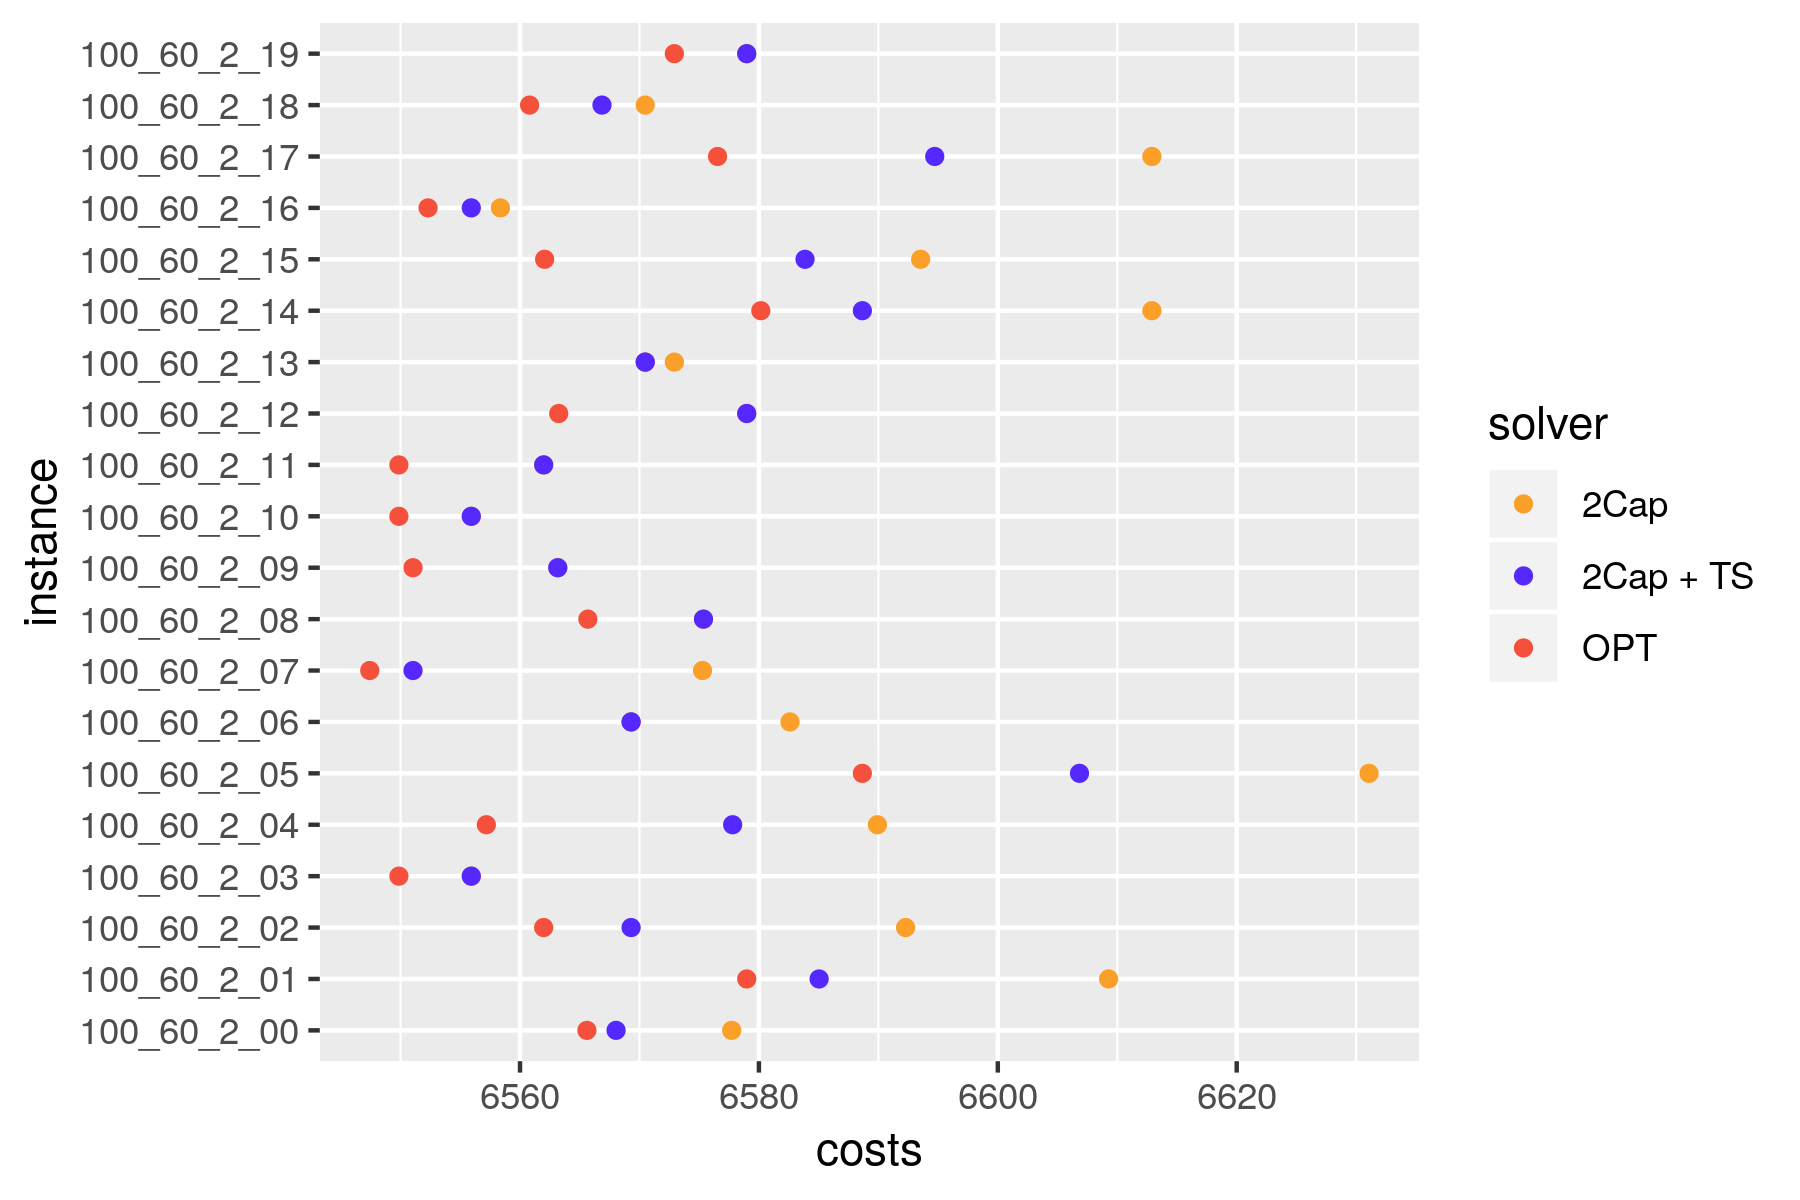
\includegraphics[width=\textwidth]{img/imp_b=2_s_costs.png}
\caption{\textsc{Kosten}}
\label{fig:imp_b=2_s_costs}
\end{subfigure}
\hfill
\begin{subfigure}[b]{0.49\textwidth}
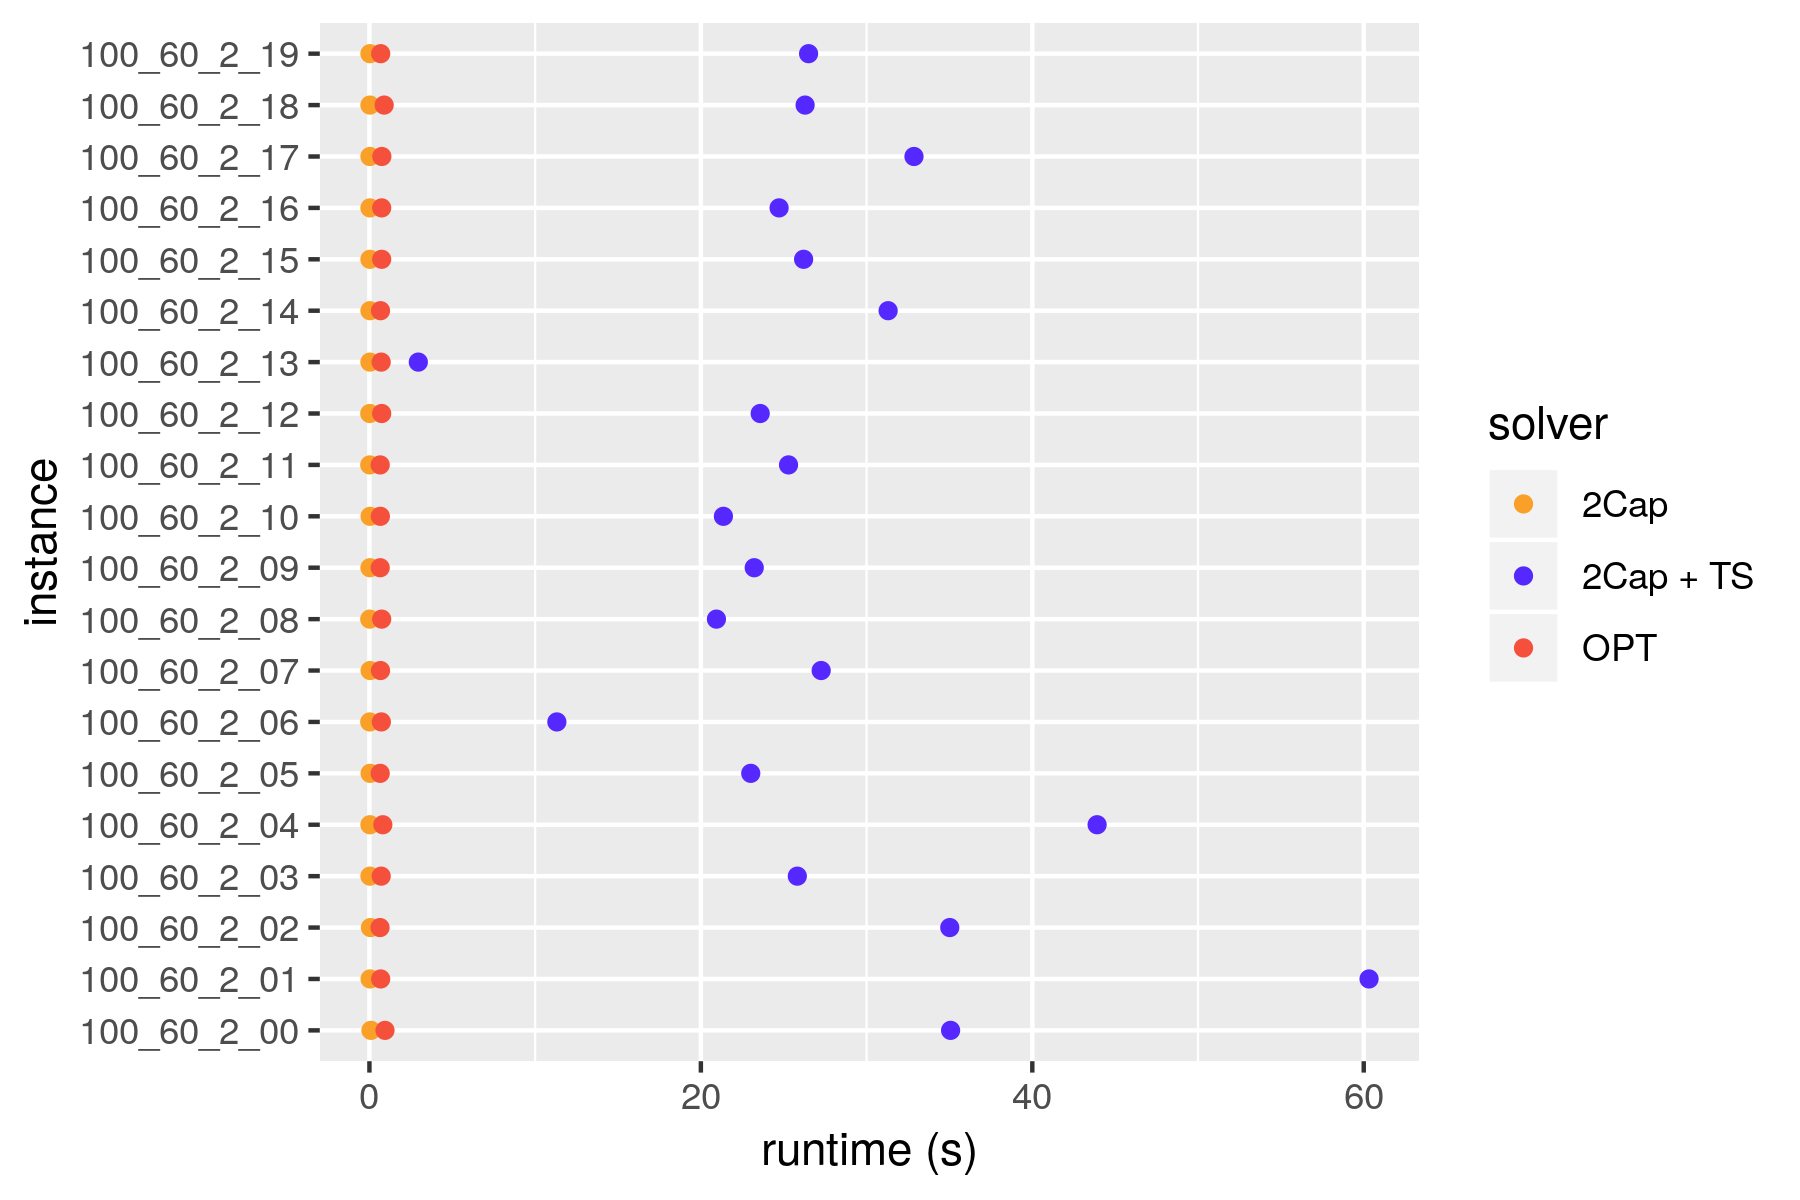
\includegraphics[width=\textwidth]{img/imp_b=2_s_runtimes.png}
\caption{\textsc{Laufzeiten}}
\label{fig:imp_b=2_s_runtimes}
\end{subfigure}
\caption{\textsc{Ergebnisse der Verbesserung $b = 2$ (s)}.}
\label{fig:imp_res_b=2_s}
\end{figure}

In der Kategorie der mittelgroßen $b = 2$ Instanzen werden die Lösungen für $12$ der $20$ Instanzen durch
die Tabu-Suche verbessert und erreichen daher eine weitere Annäherung an die optimalen Zielfunktionswerte,
wobei ein solcher in dieser Kategorie in keinem Fall ermittelt wird (vgl. Abb. \ref{fig:imp_b=2_m_costs}).
Die durchschnittliche prozentuale Abweichung vom Optimum reduziert sich dabei von $0.06 \%$ auf $0.05 \%$.
Wie man der Darstellung der Laufzeiten in Abb. \ref{fig:imp_b=2_m_runtimes} entnehmen kann, werden die
Laufzeiten der Kombination aus konstruktiver Heuristik und Tabu-Suche vom exakten Solver, verglichen
mit der Kategorie der kleinen Instanzen, etwas weniger deutlich unterboten. Der Unterschied ist mit
durchschnittlich $37.49s$ bei \textsc{OPT} im Vergleich zu durchschnittlich $128.0s$ bei \textsc{2Cap + TS}
jedoch weiterhin signifikant.

\begin{figure}[H]
\centering
\begin{subfigure}[b]{0.49\textwidth}
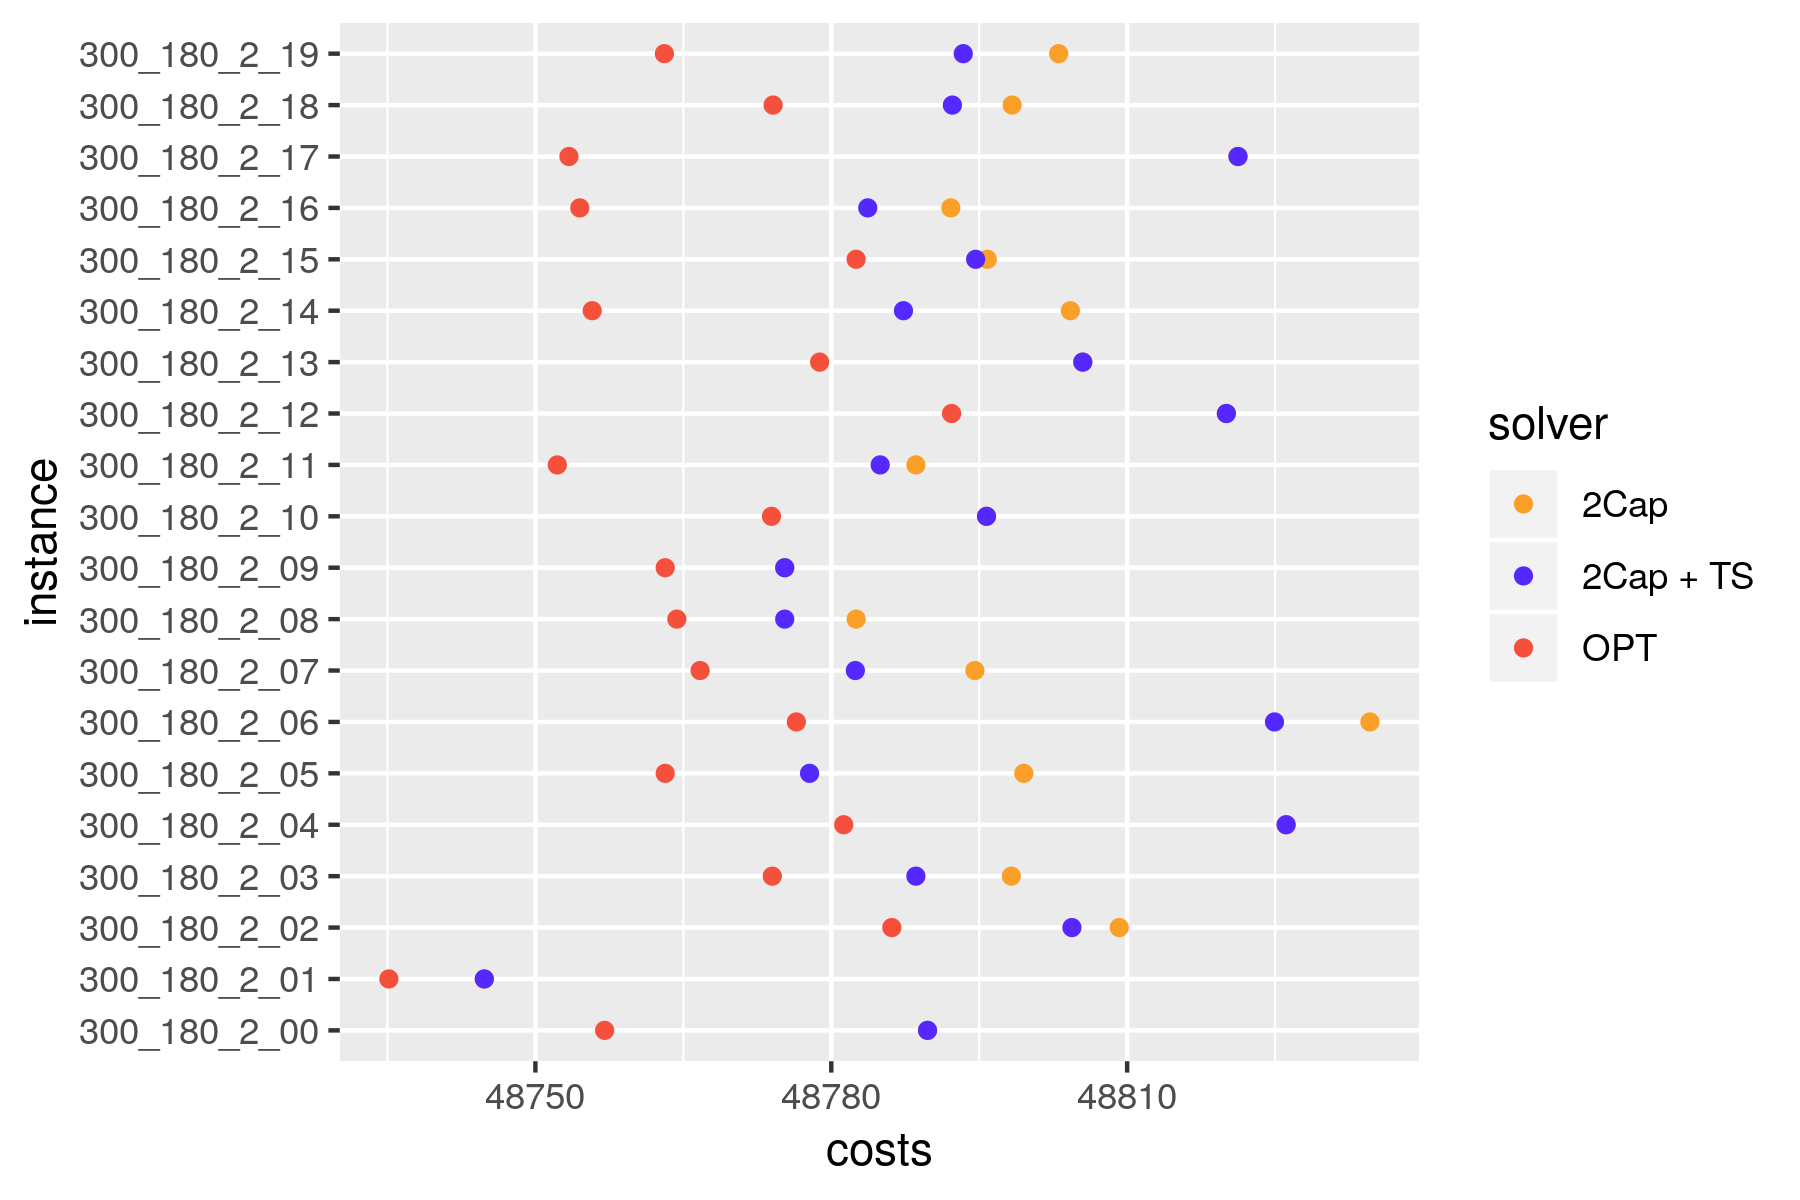
\includegraphics[width=\textwidth]{img/imp_b=2_m_costs.png}
\caption{\textsc{Kosten}}
\label{fig:imp_b=2_m_costs}
\end{subfigure}
\hfill
\begin{subfigure}[b]{0.49\textwidth}
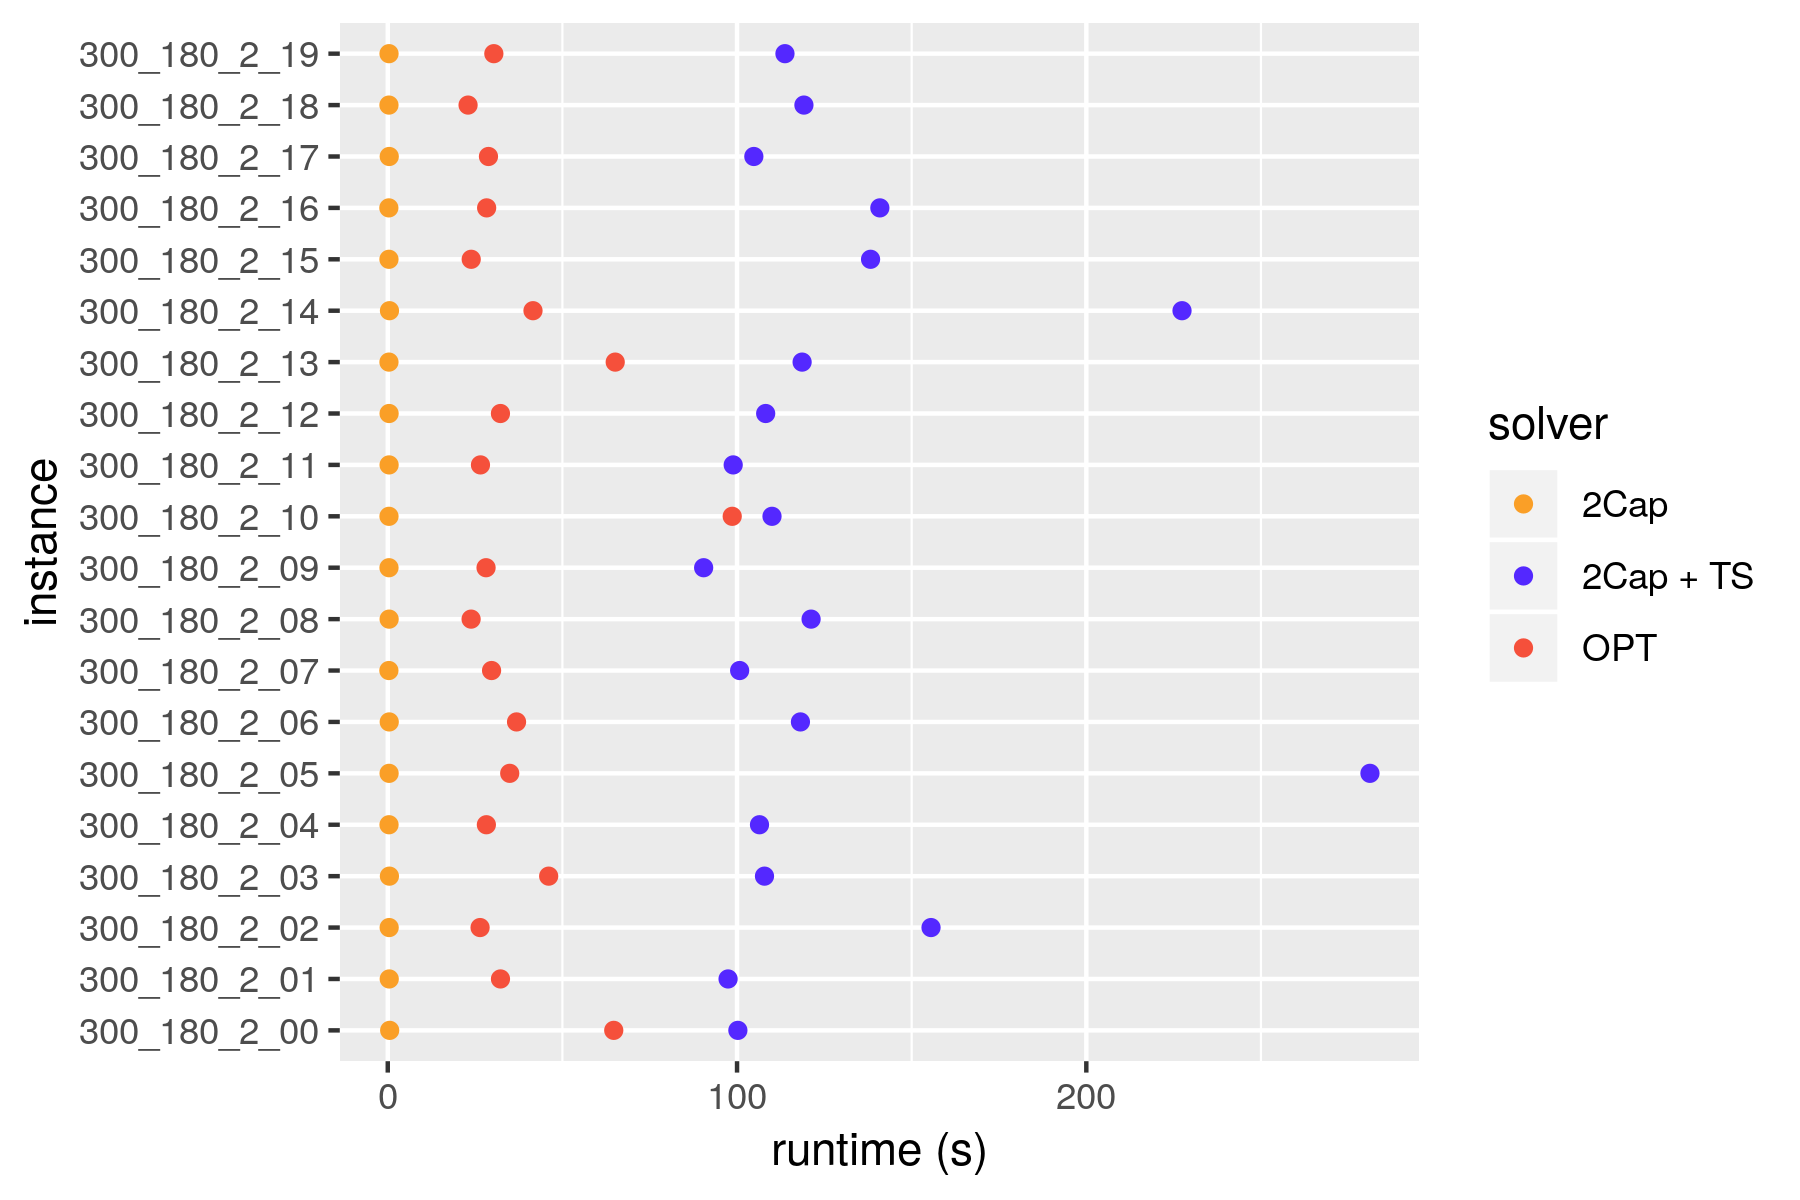
\includegraphics[width=\textwidth]{img/imp_b=2_m_runtimes.png}
\caption{\textsc{Laufzeiten}}
\label{fig:imp_b=2_m_runtimes}
\end{subfigure}
\caption{\textsc{Ergebnisse der Verbesserung $b = 2$ (m)}.}
\label{fig:imp_res_b=2_m}
\end{figure}

In der Kategorie der großen $b = 2$ Instanzen werden die Lösungen für ein Viertel der Instanzen durch
die Tabu-Suche verbessert (vgl. Abb. \ref{fig:imp_b=2_l_costs}).
Mit Instanz $03$ wird in einem Fall eine Optimallösung ermittelt. Diese wurde jedoch bereits durch die
konstruktive Heuristik generiert, weshalb sie von der Tabu-Suche nicht weiter verarbeitet wird
(vgl. Abb. \ref{fig:imp_b=2_l_runtimes}). Die durchschnittliche prozentuale Abweichung vom Optimum reduziert
sich durch die Anwendung der Tabu-Suche in dieser Kategorie nur marginal, da in vergleichsweise wenigen
Fällen eine Verbesserung stattfindet.
Wie man der Darstellung der Laufzeiten in Abb. \ref{fig:imp_b=2_l_runtimes} entnehmen kann, unterbietet die
Kombination aus Anwendung der konstruktiven Heuristik und anschließender Verbesserung durch die Tabu-Suche
den exakten Solver in dieser Kategorie in jedem Fall. \textsc{OPT} benötigt im Durchschnitt $687.99s$,
während \textsc{2Cap + TS} eine durchschnittliche Laufzeit von $208.8s$ besitzt.

\begin{figure}[H]
\centering
\begin{subfigure}[b]{0.49\textwidth}
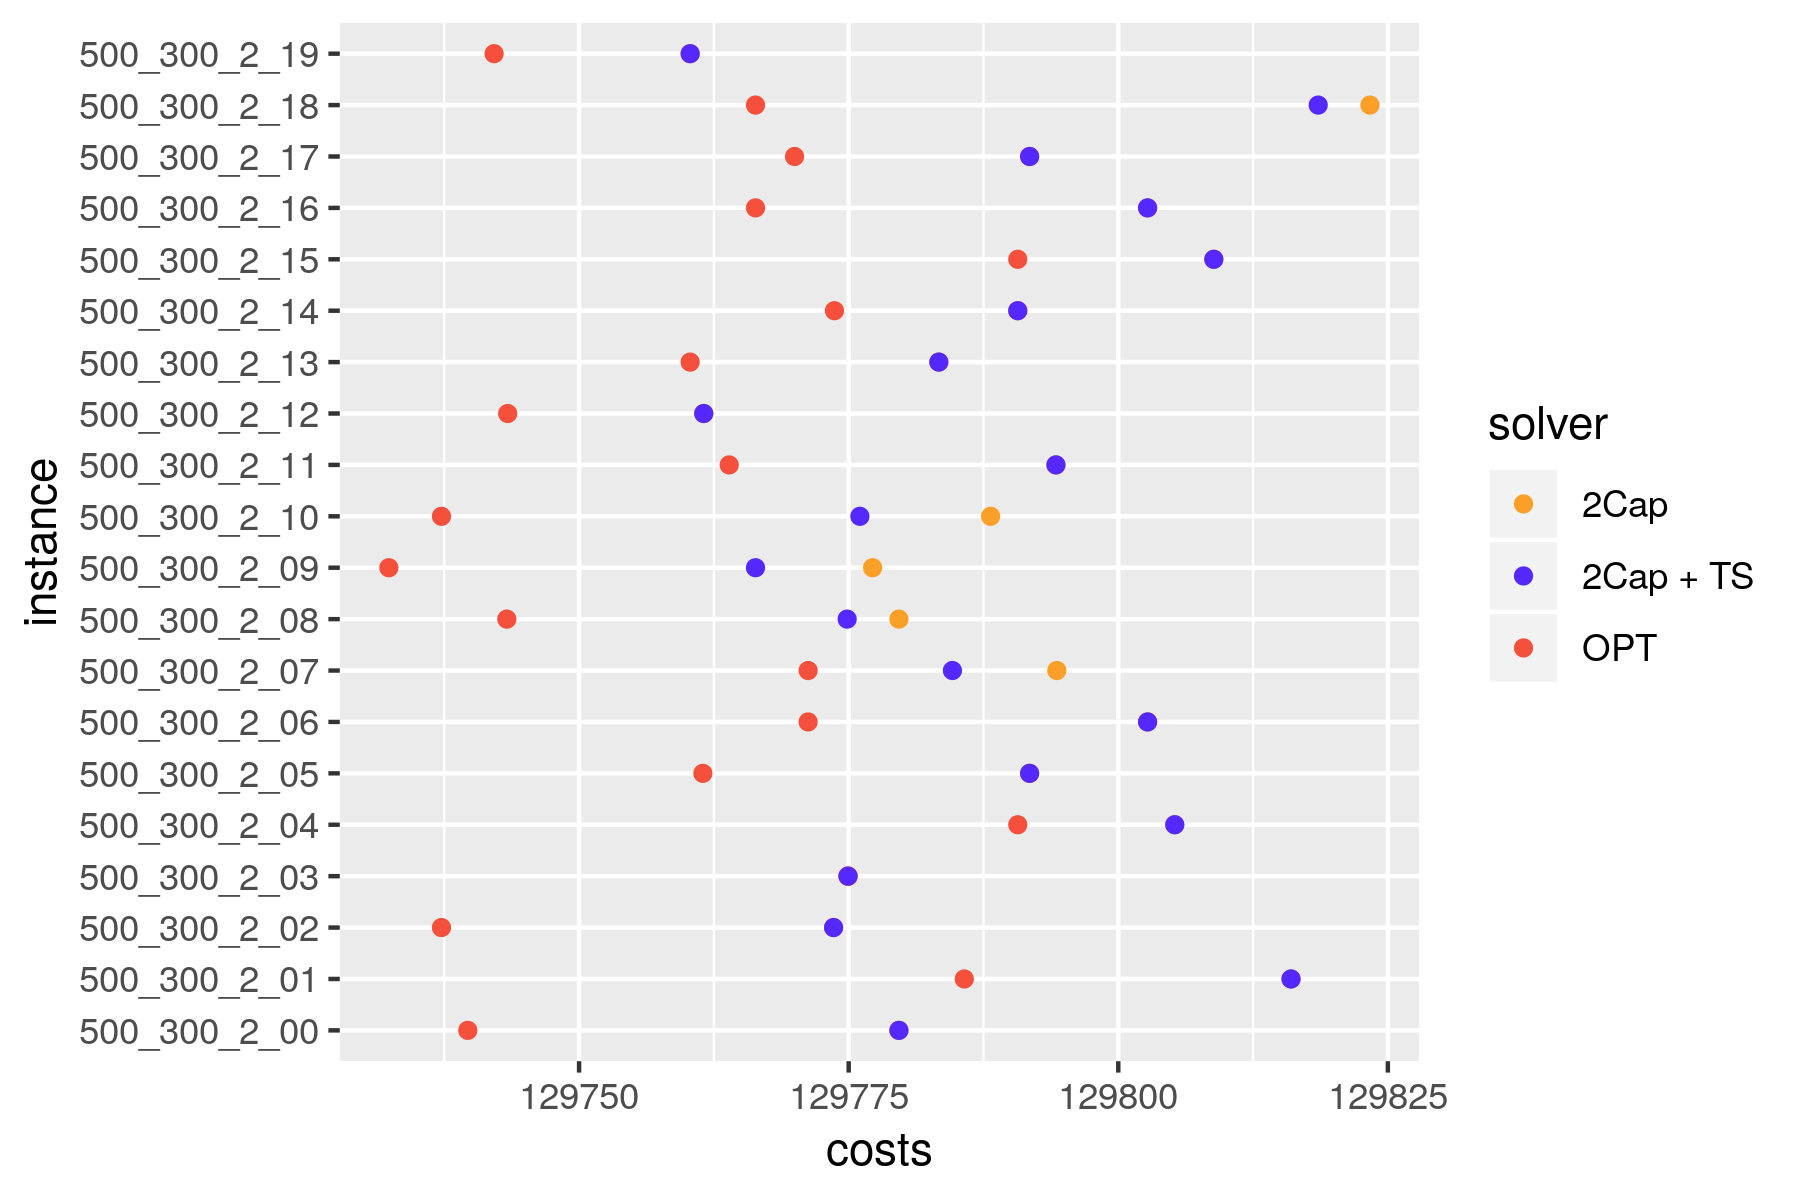
\includegraphics[width=\textwidth]{img/imp_b=2_l_costs.png}
\caption{\textsc{Kosten}}
\label{fig:imp_b=2_l_costs}
\end{subfigure}
\hfill
\begin{subfigure}[b]{0.49\textwidth}
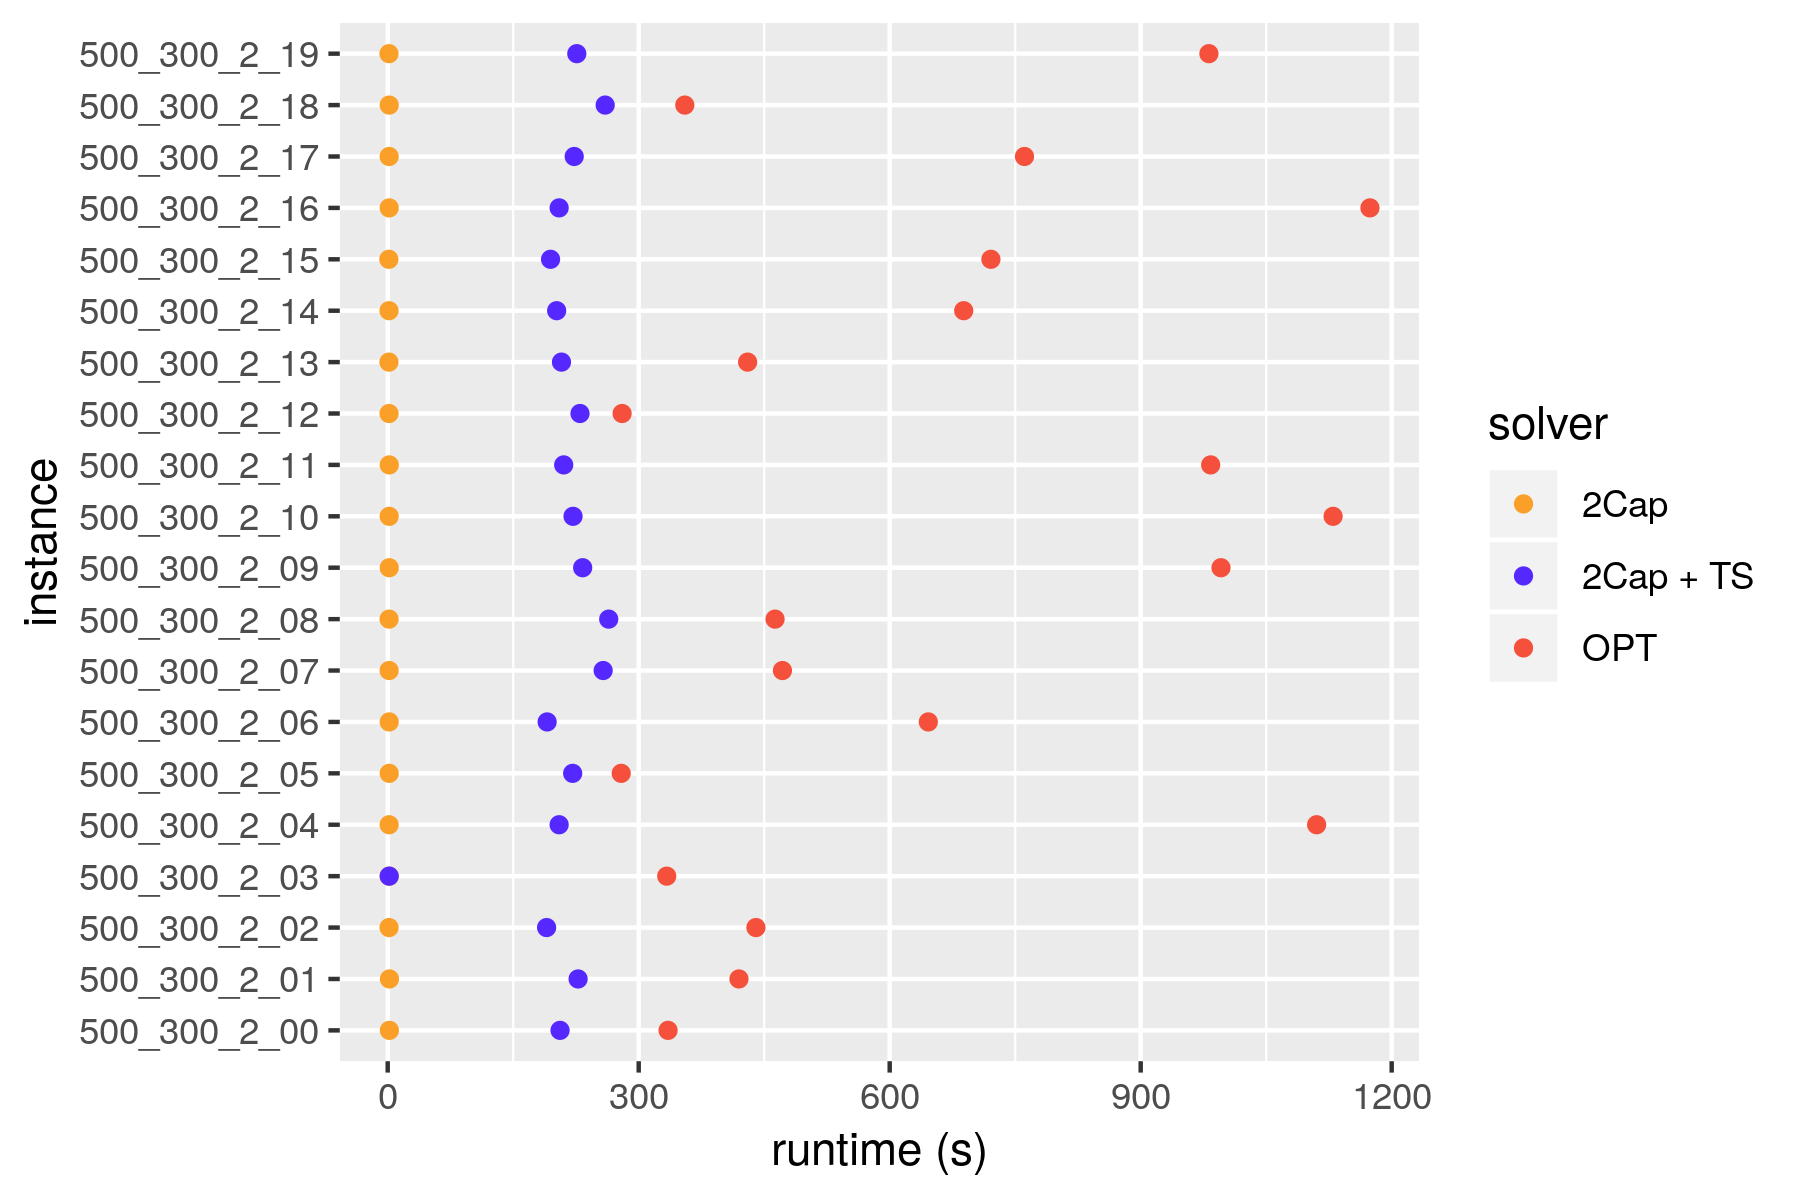
\includegraphics[width=\textwidth]{img/imp_b=2_l_runtimes.png}
\caption{\textsc{Laufzeiten}}
\label{fig:imp_b=2_l_runtimes}
\end{subfigure}
\caption{\textsc{Ergebnisse der Verbesserung $b = 2$ (l)}.}
\label{fig:imp_res_b=2_l}
\end{figure}

Nachdem sämtliche Kategorien für eine Stack-Kapazität von $b = 2$ betrachtet wurden,
geht es nun um die Verbesserung der zuvor generierten Lösungen für Instanzen von Stacking-Problemen
mit Stacks der Kapazität $b = 3$. In den Diagrammen wird die Kombination aus Anwendung der entsprechenden konstruktiven Heuristik und anschließender Anwendung der Tabu-Suche mit \textsc{3Cap + TS} abgekürzt.

In der Kategorie der kleinen $b = 3$ Instanzen werden die Lösungen für $9$ der $20$ Instanzen durch
die Tabu-Suche verbessert (vgl. Abb. \ref{fig:imp_b=3_s_costs}).
Mit den Instanzen $00$ und $11$ werden in zwei Fällen Optimallösungen ermittelt, wobei die Optimallösung
für Instanz $00$ bereits durch die konstruktive Heuristik generiert wurde. Die Optimallösung für Instanz $11$
wurde dagegen im Zuge einer erheblichen Verbesserung durch die Tabu-Suche generiert.
Die durchschnittliche prozentuale Abweichung vom Optimum reduziert sich durch die Anwendung der Tabu-Suche
von $0.20 \%$ auf $0.14 \%$.
Wie in der Darstellung der Laufzeiten in Abb. \ref{fig:imp_b=3_s_runtimes} zu erkennen ist, gehen die benötigten Laufzeiten der Tabu-Suche in dieser Kategorie, wie bereits in der Kategorie der kleinen $b = 2$ Instanzen,
weit über jene der Heuristik und des exakten Solvers hinaus.
Die durchschnittliche Laufzeit von \textsc{OPT} beträgt $1.15s$, während die Laufzeit von \textsc{3Cap + TS} durchschnittlich $60.9s$ beträgt. Es geht allerdings in dieser Kategorie erneut nicht darum, die Laufzeit des exakten
Solvers zu unterbieten, sondern darum, einen guten Kompromiss aus einer geringen Laufzeit und einer großen Kostenreduktion zu finden, worauf die in Abschnitt \ref{sec:tabu_search_config} vorgestellte Konfiguration
abzielt.

\begin{figure}[H]
\centering
\begin{subfigure}[b]{0.49\textwidth}
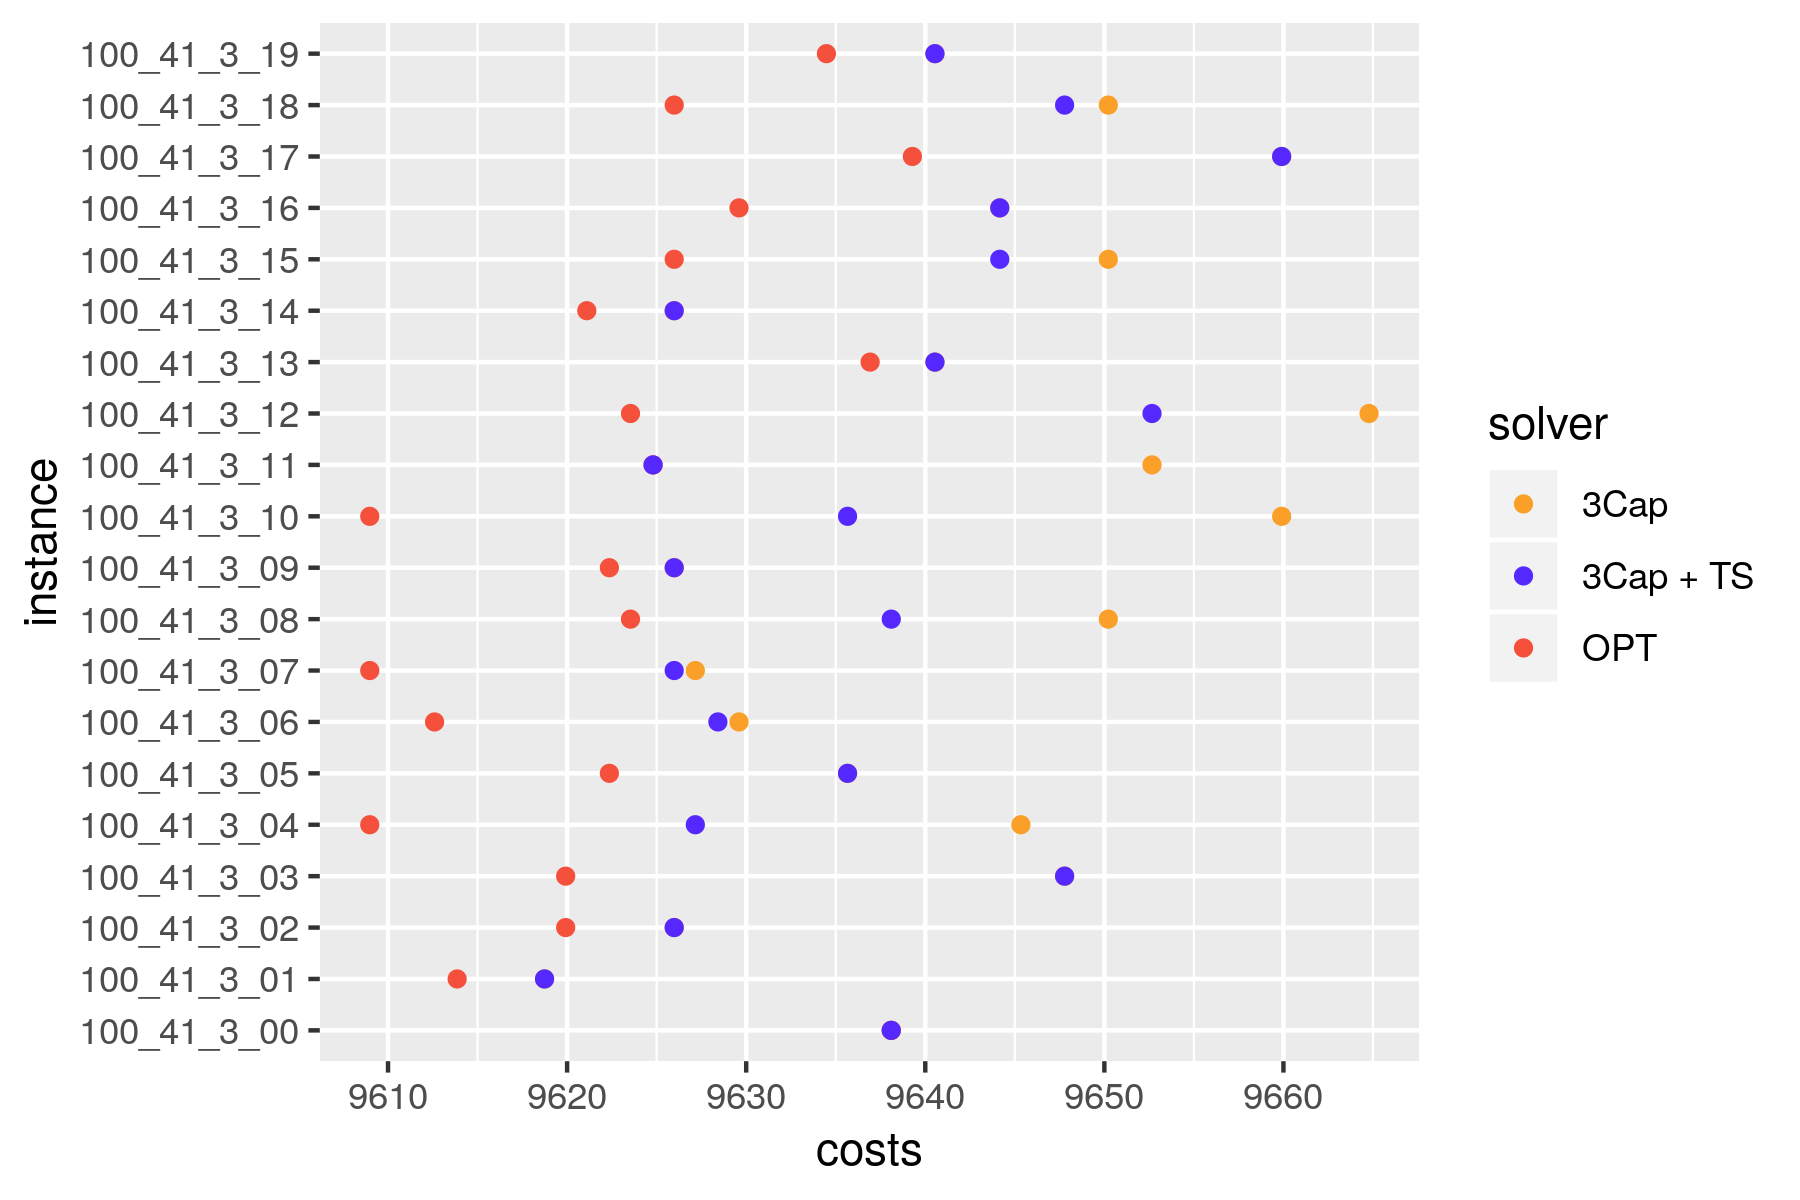
\includegraphics[width=\textwidth]{img/imp_b=3_s_costs.png}
\caption{\textsc{Kosten}}
\label{fig:imp_b=3_s_costs}
\end{subfigure}
\hfill
\begin{subfigure}[b]{0.49\textwidth}
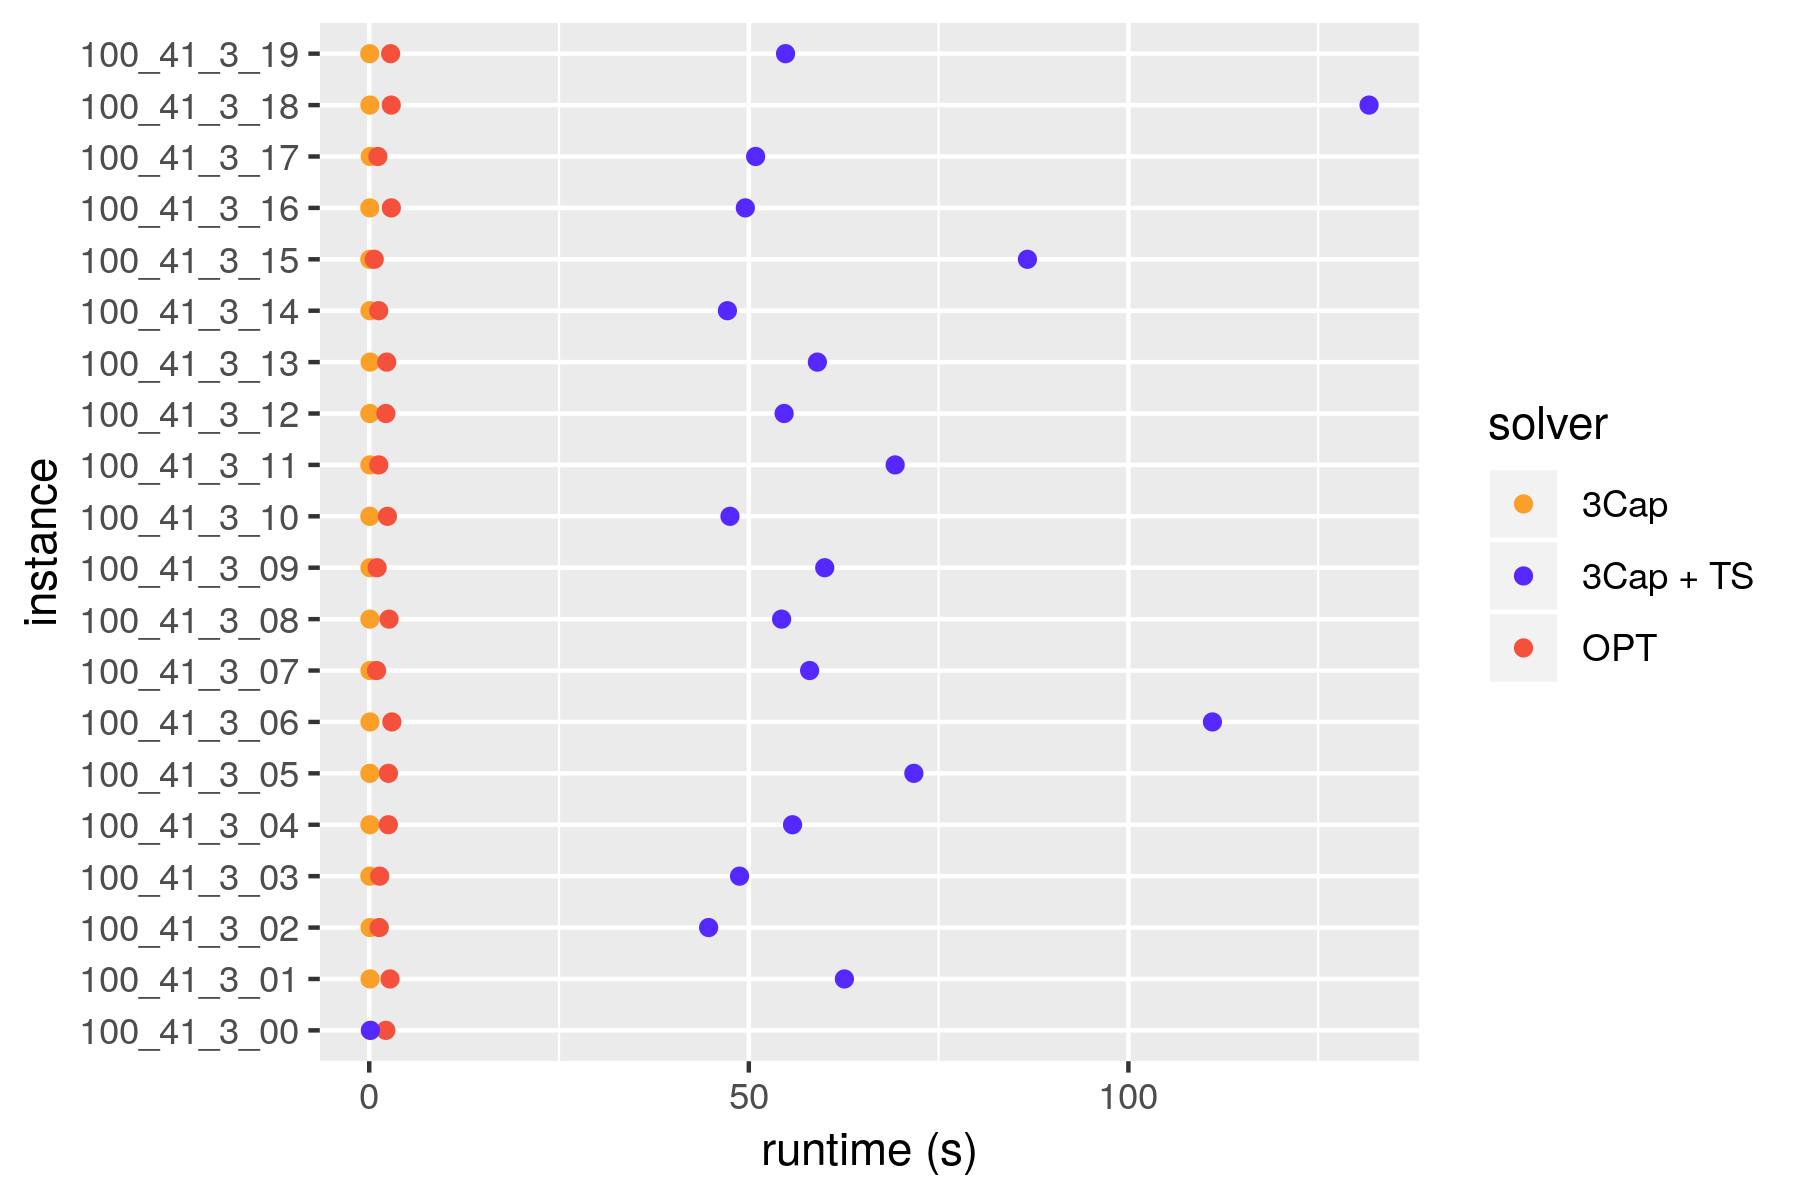
\includegraphics[width=\textwidth]{img/imp_b=3_s_runtimes.png}
\caption{\textsc{Laufzeiten}}
\label{fig:imp_b=3_s_runtimes}
\end{subfigure}
\caption{\textsc{Ergebnisse der Verbesserung $b = 3$ (s)}.}
\label{fig:imp_res_b=3_s}
\end{figure}

Abbildung \ref{fig:imp_b=3_m_costs} ist zu entnehmen, dass in der Kategorie der mittelgroßen $b = 3$ Instanzen
die Lösungen für $11$ der $20$ Instanzen durch die Tabu-Suche verbessert werden.
Die einzige resultierende Optimallösung wurde bereits von der konstruktiven Heuristik generiert.
Bei den Instanzen $08$ und $12$ wurde durch die Verbesserung der Tabu-Suche annähernd der optimale
Zielfunktionswert erreicht. Die durchschnittliche prozentuale Abweichung vom Optimum reduziert sich
durch die Anwendung der Tabu-Suche von $0.03 \%$ auf $0.02 \%$.
Wie in der Darstellung der Laufzeiten in Abb. \ref{fig:imp_b=3_m_runtimes} zu erkennen ist,
ist der exakte Solver in dieser Kategorie in der Regel schneller als die Tabu-Suche, wobei es mit
den Instanzen $01, 02, 13$ und $14$ einige Ausnahmen gibt, bei denen die Kombination aus konstruktiver Heuristik
und anschließender Anwendung der Tabu-Suche schneller ist. Wenngleich die Lösung von Instanz $01$ nicht von der
Tabu-Suche verarbeitet wird, da diese bereits optimal ist. Die durchschnittliche Laufzeit von \textsc{OPT}
beträgt $163.94s$, während die Laufzeit von \textsc{3Cap + TS} durchschnittlich $391.7s$ beträgt.

\begin{figure}[H]
\centering
\begin{subfigure}[b]{0.49\textwidth}
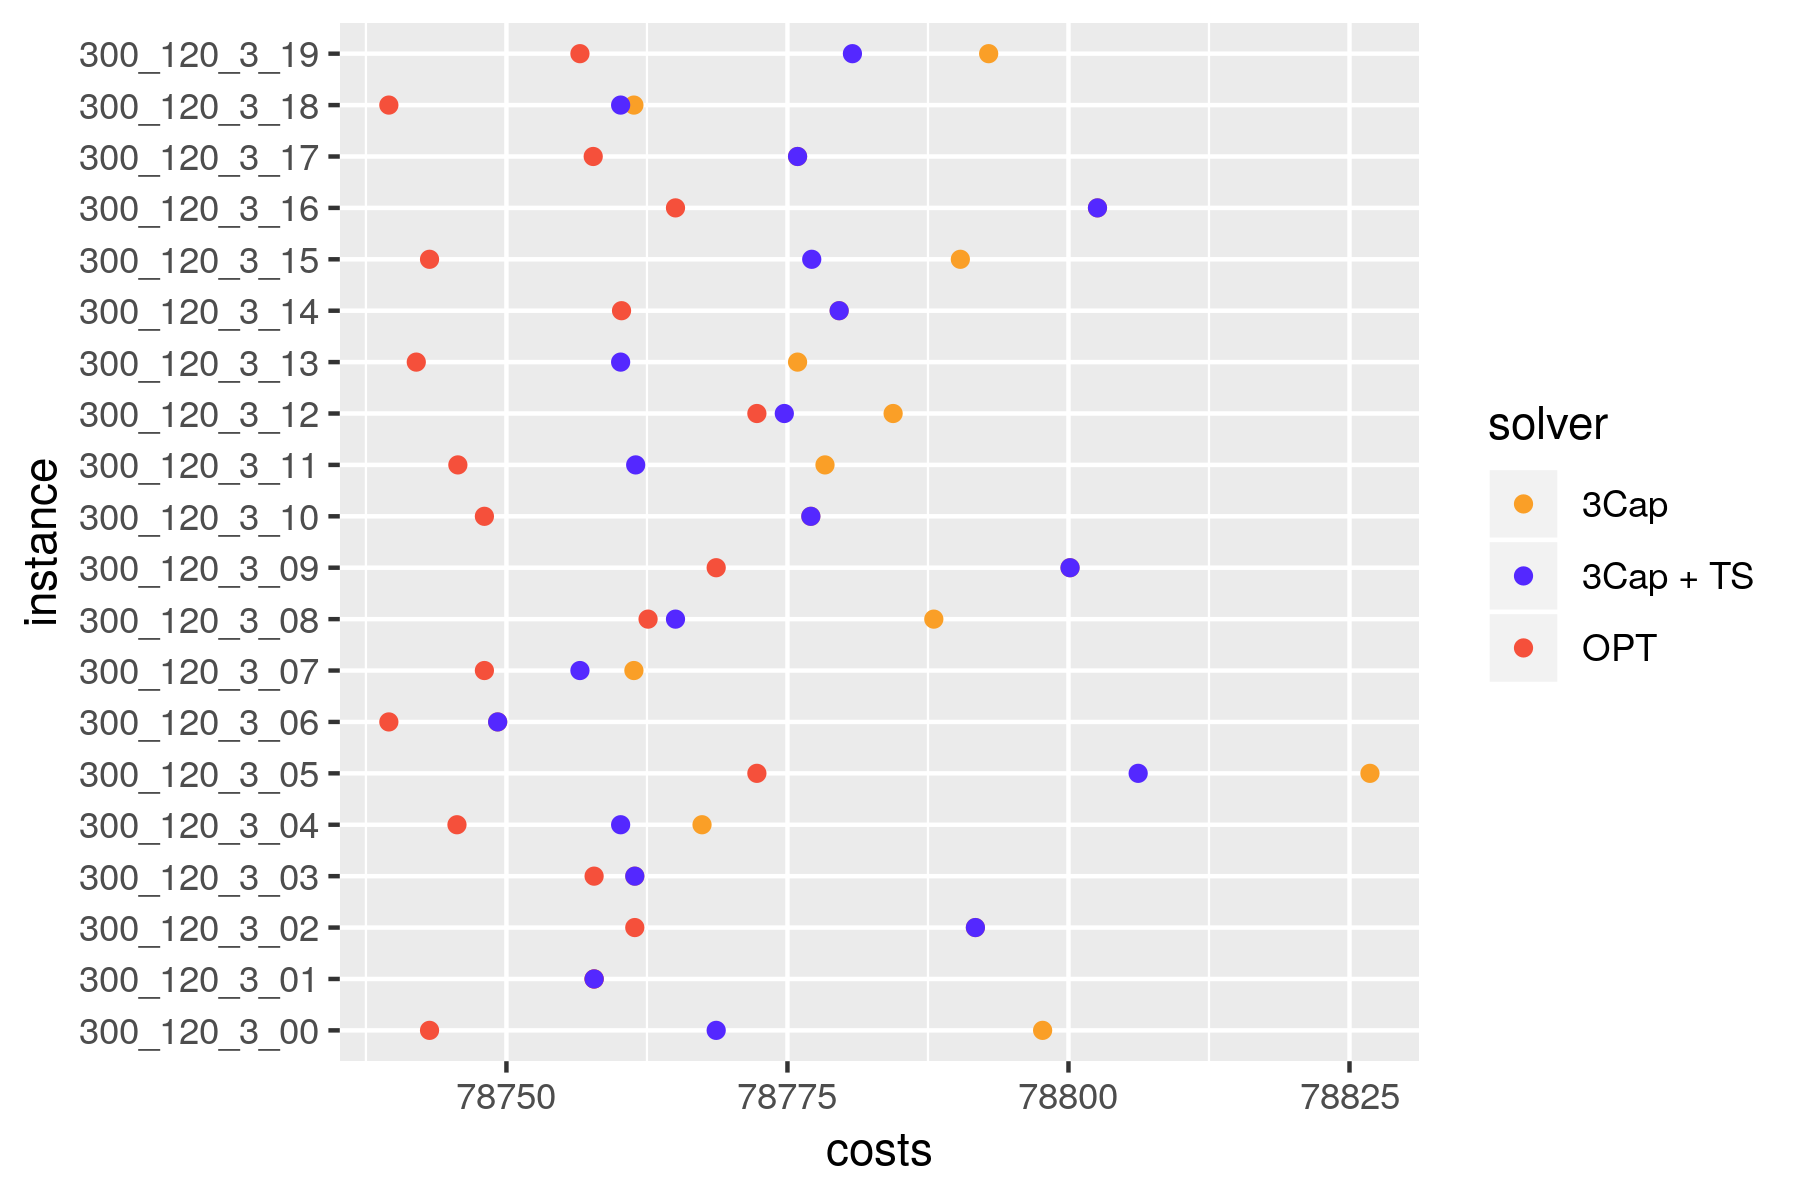
\includegraphics[width=\textwidth]{img/imp_b=3_m_costs.png}
\caption{\textsc{Kosten}}
\label{fig:imp_b=3_m_costs}
\end{subfigure}
\hfill
\begin{subfigure}[b]{0.49\textwidth}
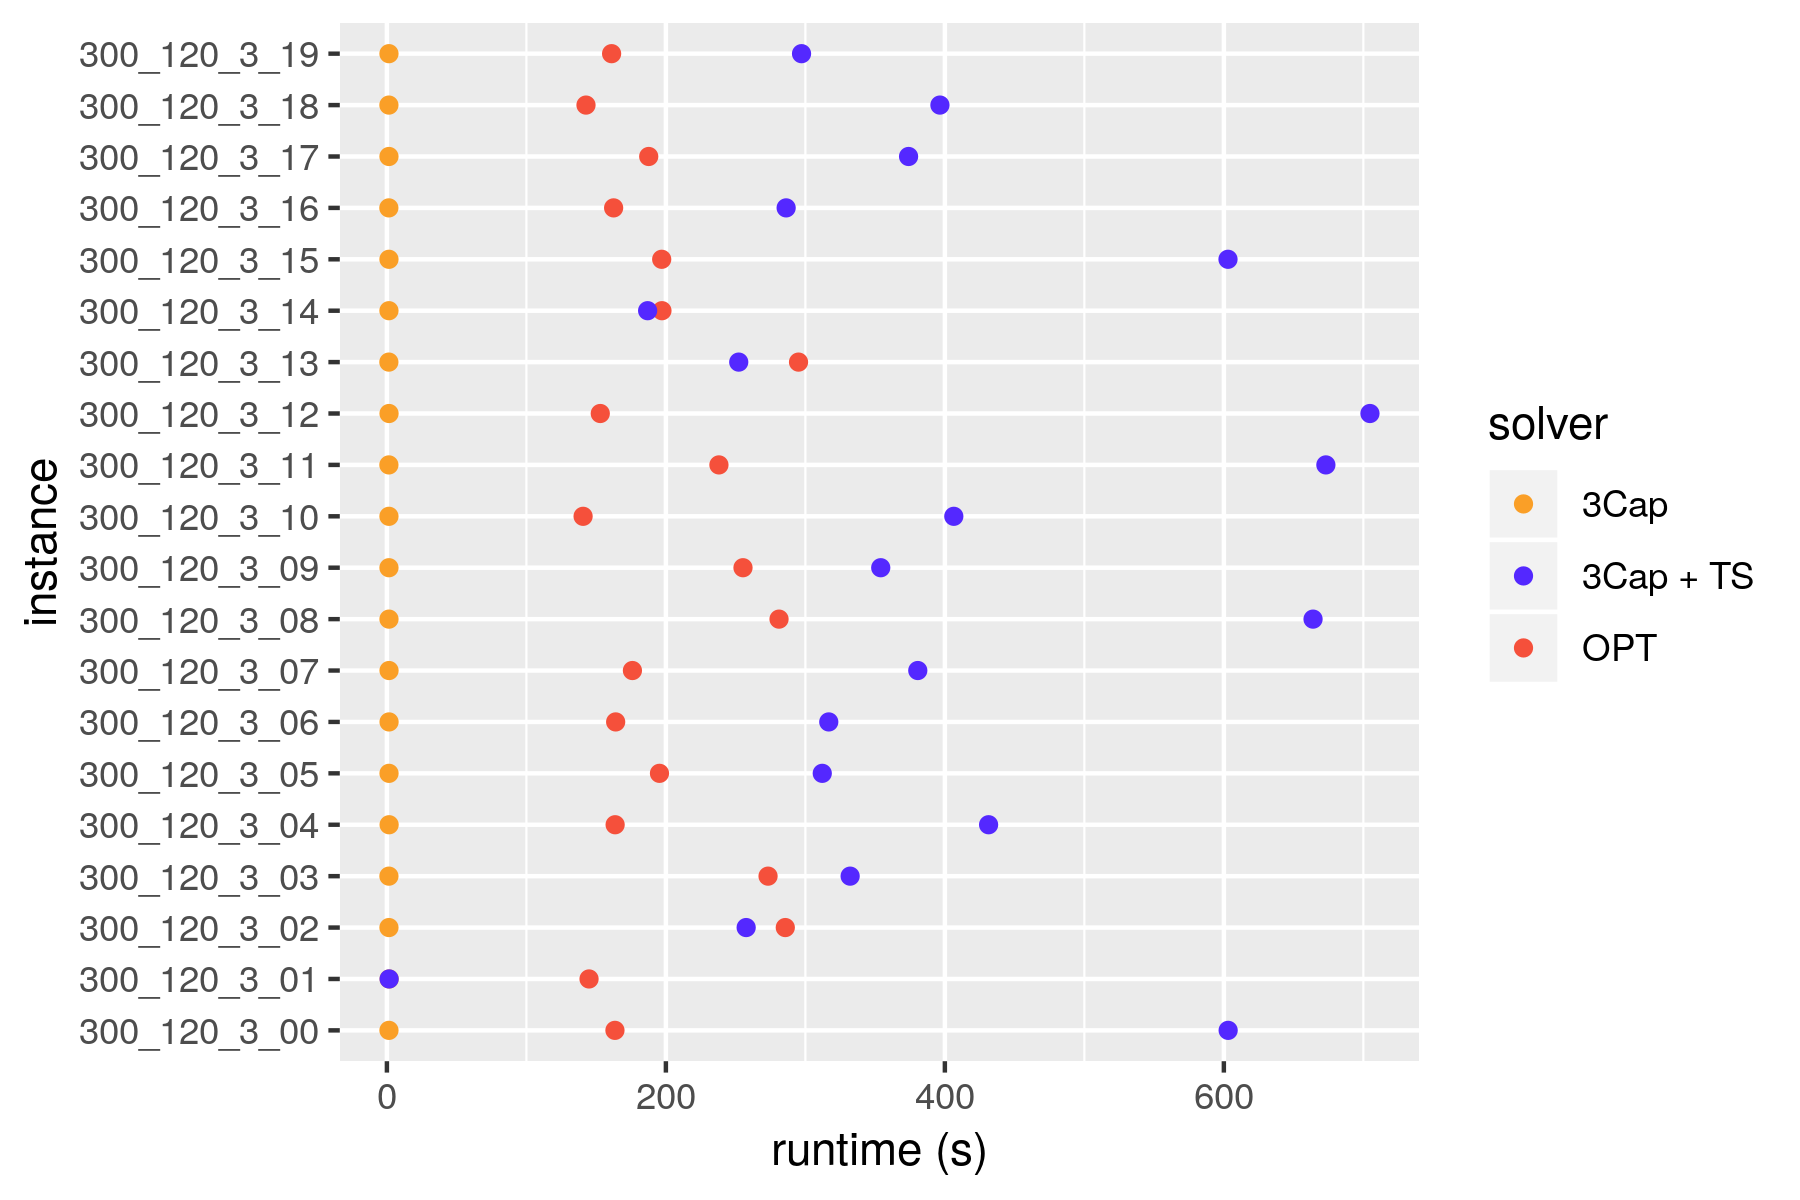
\includegraphics[width=\textwidth]{img/imp_b=3_m_runtimes.png}
\caption{\textsc{Laufzeiten}}
\label{fig:imp_b=3_m_runtimes}
\end{subfigure}
\caption{\textsc{Ergebnisse der Verbesserung $b = 3$ (m)}.}
\label{fig:imp_res_b=3_m}
\end{figure}

In der Kategorie der großen $b = 3$ Instanzen werden die Lösungen für $12$ der $20$ Instanzen durch
die Tabu-Suche verbessert (vgl. Abb. \ref{fig:imp_b=3_l_costs}).
Es wird zwar keine Optimallösung gefunden, dennoch ergeben sich deutliche Verbesserungen, welche
die durchschnittliche prozentuale Abweichung vom Optimum von $0.02 \%$ auf $0.01 \%$ reduzieren.
Wie der Darstellung der Laufzeiten in Abb. \ref{fig:imp_b=3_l_runtimes} zu entnehmen ist, unterbietet die
Kombination aus Anwendung der konstruktiven Heuristik und anschließender Verbesserung durch die Tabu-Suche
den exakten Solver in dieser Kategorie in jedem Fall. \textsc{OPT} benötigt im Durchschnitt $1139.19s$,
während \textsc{3Cap + TS} eine durchschnittliche Laufzeit von $449.6s$ besitzt.

\begin{figure}[H]
\centering
\begin{subfigure}[b]{0.49\textwidth}
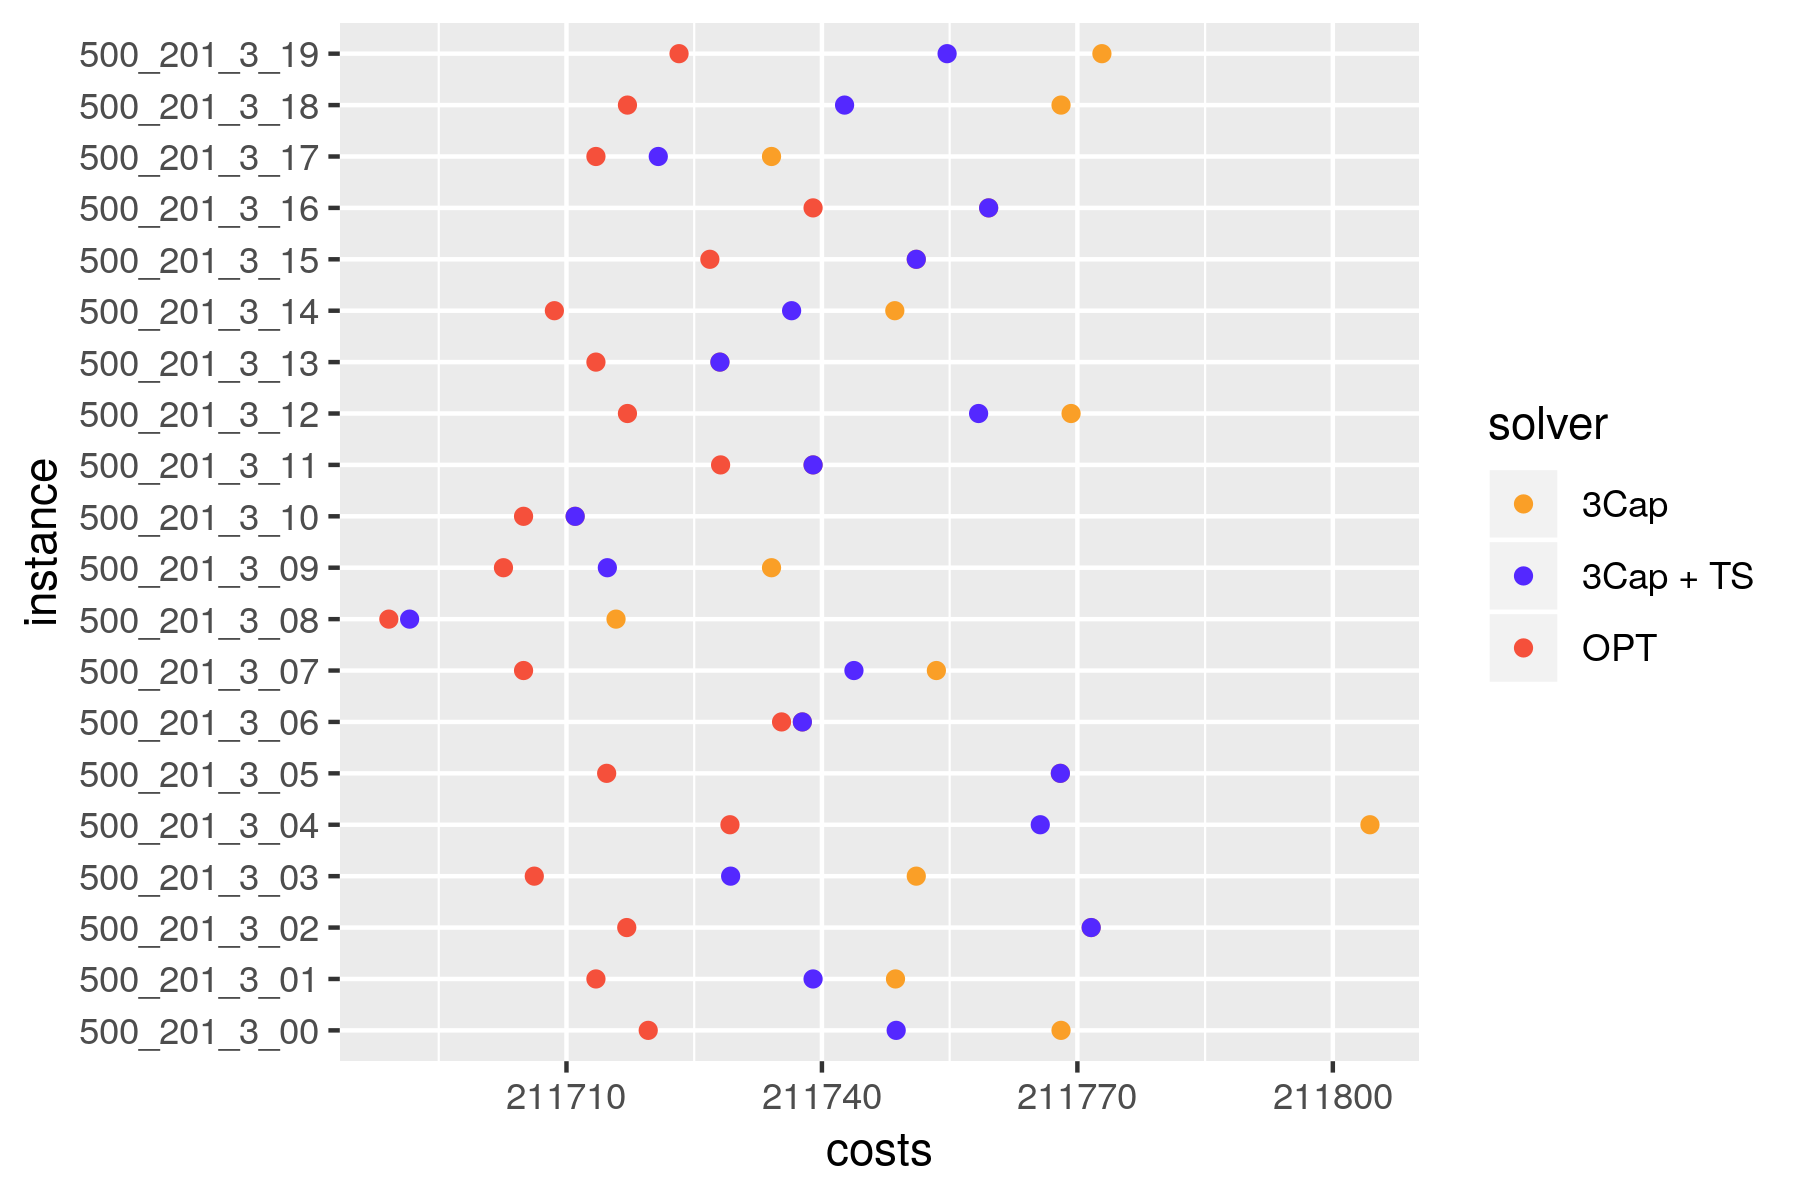
\includegraphics[width=\textwidth]{img/imp_b=3_l_costs.png}
\caption{\textsc{Kosten}}
\label{fig:imp_b=3_l_costs}
\end{subfigure}
\hfill
\begin{subfigure}[b]{0.49\textwidth}
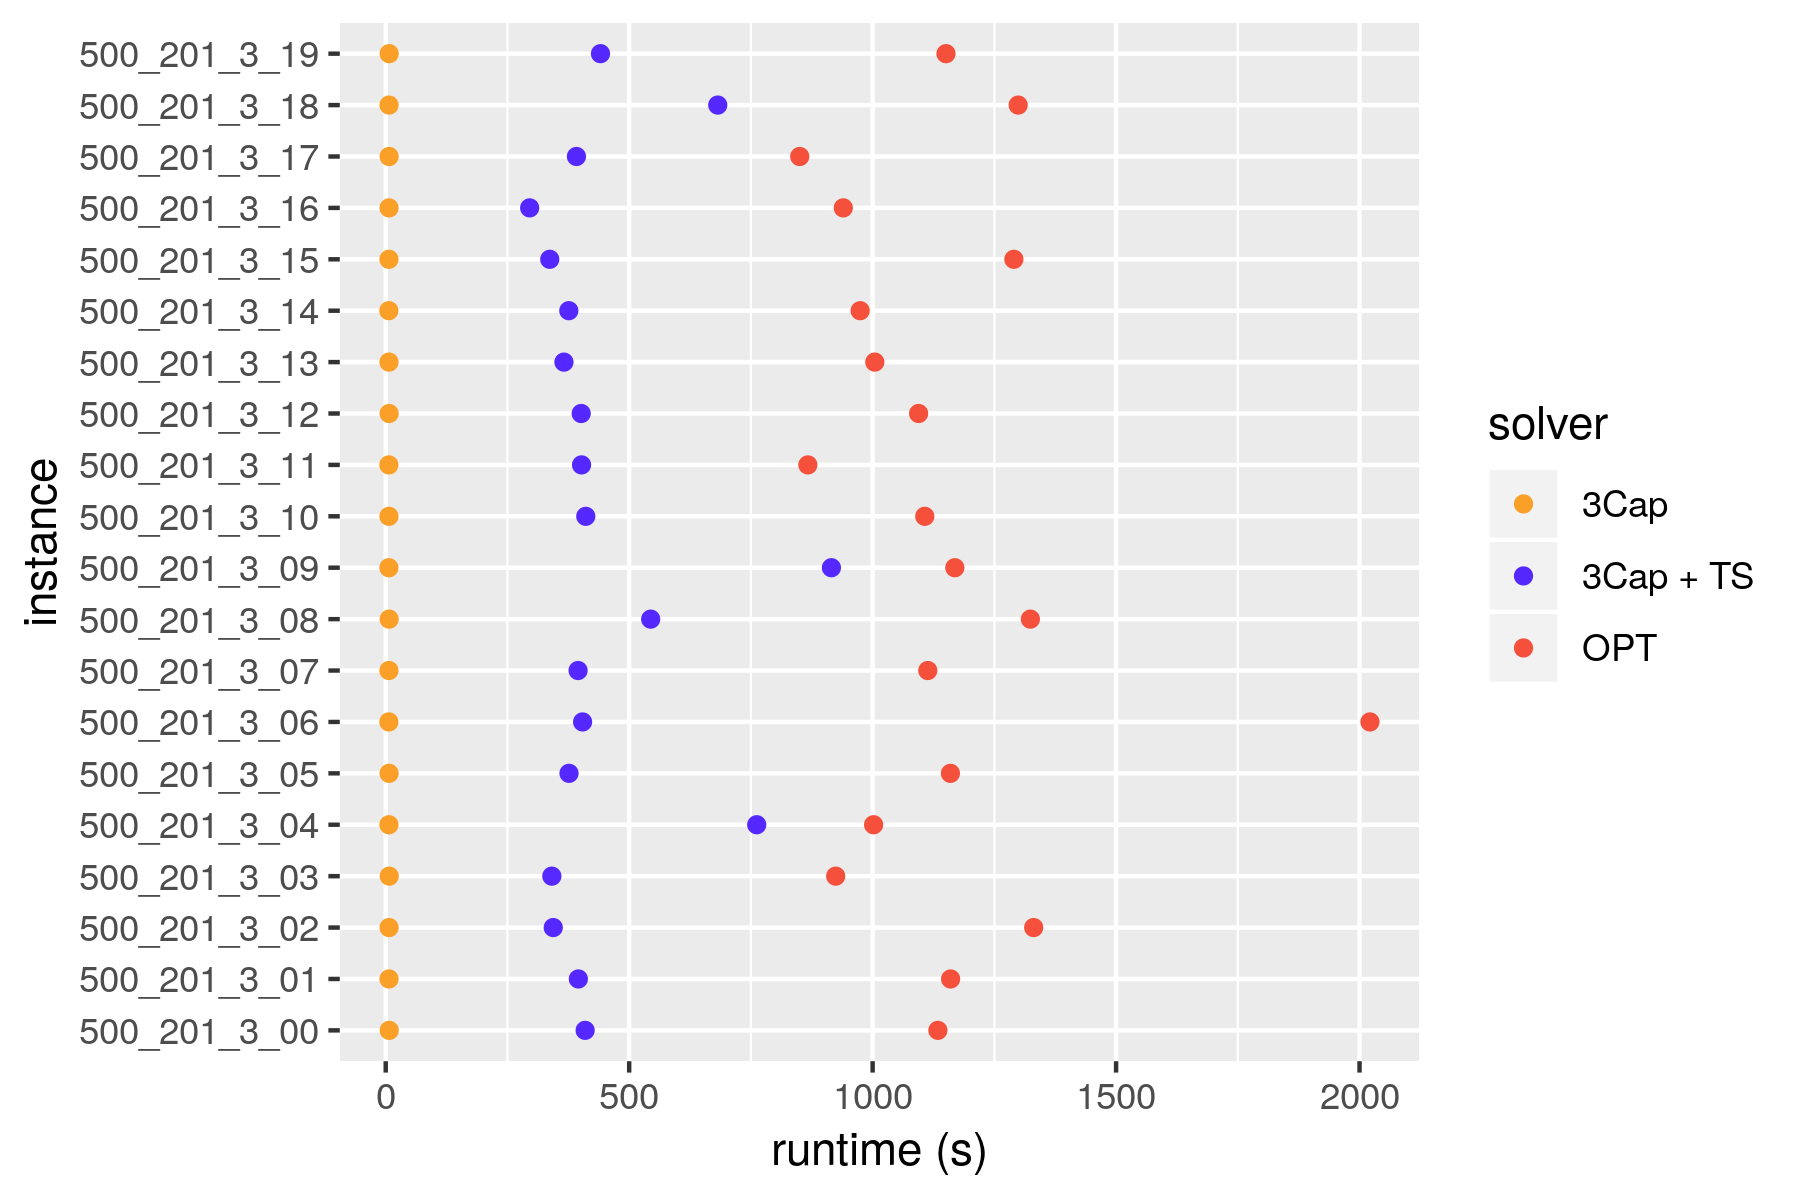
\includegraphics[width=\textwidth]{img/imp_b=3_l_runtimes.png}
\caption{\textsc{Laufzeiten}}
\label{fig:imp_b=3_l_runtimes}
\end{subfigure}
\caption{\textsc{Ergebnisse der Verbesserung $b = 3$ (l)}.}
\label{fig:imp_res_b=3_l}
\end{figure}

Zusammenfassend lässt sich sagen, dass das Verbesserungsverfahren sowohl für $b = 2$,
als auch für $b = 3$ in der Kategorie der kleinen Instanzen zu lange Laufzeiten besitzt,
um mit den exakten Verfahren konkurrieren zu können.
Wie bereits in den Abschnitten \ref{sec:solver_comp_b=2} und \ref{sec:solver_comp_b=3} erläutert,
herrscht in dieser Kategorie allerdings ohnehin kein Bedarf für eine heuristische Lösung,
sofern ein exakter Solver mit derart geringen Laufzeiten zur Verfügung steht.
Steht ein solcher nicht zur Verfügung, so ist die konstruktive Heuristik ohne Anwendung der
Tabu-Suche bei sehr geringen Laufzeiten und Abweichungen von den Optimalwerten eine gute Alternative.
Wird dagegen die strikte Kostenminimierung vor einer geringen Laufzeit priorisiert, so kann zusätzlich das Verbesserungsverfahren zum Einsatz kommen, welches die durchschnittlichen Kosten noch einmal in durchaus
relevantem Maße reduziert.
In der Kategorie der mittelgroßen Instanzen ist der exakte Solver ebenfalls bei beiden Stack-Kapazitäten
in der Regel schneller als die kombinierte Anwendung der konstruktiven Heuristik und der Tabu-Suche.
Dementsprechend stehen erneut die geschilderte Priorisierung der Laufzeit oder der Kostenminimierung zur
Auswahl. Auch in dieser Kategorie gelangt die Tabu-Suche zu durchaus signifikanten Verbesserungen.
In der Kategorie der großen Instanzen unterbietet die Kombination der beiden heuristischen Verfahren
in Bezug auf die Laufzeit jeweils den exakten Solver, weshalb diese eine noch flexiblere Konkurrenz
zum exakten Verfahren darstellt, weil die Tabu-Suche optional zur weiteren Kostenminimierung eingesetzt werden
kann und in jedem Fall geringere Laufzeiten erzielt werden. Ist die Laufzeit nicht kritisch und ein weiterer
Fokus auf Kostenminimierung erwünscht, so kann als Abbruchkriterium für die Tabu-Suche eine feste Laufzeit
gesetzt werden, welche beispielsweise beliebig den Laufzeiten des exakten Verfahrens angenähert werden,
oder diese bei Bedarf auch übersteigen kann. Im Wesentlichen ermöglicht die konstruktive Heuristik in
Verbindung mit der Tabu-Suche eine recht flexible Lösung individueller Szenarien. Je nach Priorisierung
der Laufzeit oder der Kostenminimierung, können sich unterschiedliche Konfigurationen als sinnvoll erweisen.

\vfill
\pagebreak

\section{Fazit und Ausblick}
\label{sec:conclusion}

Ziel dieser Arbeit war es, effiziente Lösungsverfahren für praktisch motivierte Stacking-Probleme mit Transportkosten,
wie sie beispielsweise in Lagerhallen und Container-Terminals auftreten, zu entwickeln.

Die vorgestellten konstruktiven Heuristiken lösen Stacking-Probleme mit Stacks der Kapazitäten $b = 2$ und $b = 3$,
welche in Szenarien aus der Praxis, in welchen Container gestapelt werden, häufig ausreichen, effizient mit sehr geringen Abweichungen von den Optimallösungen. In den durchgeführten Experimenten wurde deutlich, dass diese erheblich kürzere Laufzeiten besitzen als die zum Vergleich genutzten MIP-Formulierungen, welche vom kommerziellen MIP-Solver \textsc{CPLEX} gelöst wurden und bei ausreichend Laufzeit und Speicher optimale Zielfunktionswerte liefern.
Des Weiteren wurde demonstriert, dass die Heuristiken vor allem bei großen Instanzen, bei welchen die Einlagerung
von $500$ Items betrachtet wird, ihren Effizienzvorteil zeigen.
Grundsätzlich gewinnt dieser Vorteil der Heuristiken gegenüber \textsc{CPLEX} mit wachsenden Instanzgrößen
an Bedeutung, denn auch Instanzen, welche weit mehr als $500$ Items enthalten, können von den vorgestellten
konstruktiven Heuristiken effizient gelöst werden, während die von \textsc{CPLEX} gelösten MIP-Formulierungen
zunehmend an ihre Grenzen stoßen. Da ein praktischer Einsatz exakter Solver aufgrund des enormen Laufzeit- und Speicherbedarfs bei großen Instanzen nicht sinnvoll oder sogar ausgeschlossen ist, stellen die vorgestellten Heuristiken gute Alternativen dar.

Zusätzlich zu den konstruktiven Verfahren wurde mit der Tabu-Suche ein Verbesserungsverfahren entwickelt,
welches von den konstruktiven Heuristiken generierte Lösungen als Eingabe bekommt, um diese
im Laufe des Verfahrens zu verbessern. Dabei war das Ziel, einen guten Kompromiss aus geringen Laufzeiten
und großen Kostenreduktionen zu finden. Dieses Ziel wurde für die gegenwärtige Implementation der Tabu-Suche durch die geschilderte Konfiguration erreicht. In der Anwendung der Tabu-Suche wurde deutlich, dass in sämtlichen Kategorien zahlreiche signifikante Verbesserungen zu verzeichnen sind und sich die Laufzeiten in einem als akzeptabel empfundenen Rahmen, welcher eine sinnvolle Anwendung der Tabu-Suche ermöglicht, bewegen.
Dennoch gibt es durchaus Verbesserungspotenzial, es wäre beispielsweise erstrebenswert,
mehr Instanzen optimal zu lösen. Dazu kann die vorgestellte Tabu-Suche in Zukunft weiterentwickelt werden.
Idealerweise könnte eine, verglichen mit der gegenwärtigen, kleinere Nachbarschaft definiert werden, welche die Zusammenhangseigenschaft erfüllt.
Außerdem benötigt das systematische Durchsuchen des Lösungsraums aus theoretischer Perspektive weniger Zeit
als das bisher verwendete randomisierte Verfahren, weshalb sich dies auch praktisch als vorteilhaft erweisen könnte.
Auch die Betrachtung einer weiteren Lösungsrepräsentation, in welcher Lösungen durch Partitionen kompatibler Items
gegeben sind, sollte untersucht werden. Die Items sind in dieser Repräsentation initial noch
keinem Stack zugewiesen. Die Zuweisung der Partitionen zu Stacks findet erst im Anschluss an das Verfahren statt, indem ein Minimum-Weight-Bipartite-Perfect-Matching zwischen Partitionen und Stacks ermittelt wird. Dabei handelt es sich um eine optimale Zuweisung. Um jedem Item einen Level innerhalb eines Stacks zuzuweisen, müssen die Partitionen
analog zum letzten Schritt der konstruktiven Heuristiken lediglich basierend auf den transitiven Stacking-Constraints
sortiert werden. Ein Umsetzen dieser Ansätze war im Rahmen der vorliegenden Arbeit nicht mehr möglich, kann sich
jedoch in Zukunft als lohnenswert erweisen.

Im Verlauf dieser Arbeit haben sich an vielen Stellen, vor allem durch unterschiedliche praktisch motivierte Szenarien, Konfigurationsmöglichkeiten ergeben, welche weitere, zukünftige Betrachtungen sinnvoll erscheinen lassen.
Die betrachteten unteren Schranken haben beispielsweise gezeigt, dass der Einfluss der Stacking-Constraints mit der ausschließlich verwendeten zweiten Variante der Stacking-Constraint-Generierung stets recht gering ausfällt. Dementsprechend könnten Experimente mit der ersten Variante der Stacking-Constraint-Generierung von Interesse sein.
Auch der Einfluss der Dichte der Stacking-Matrix, der Anzahl der zur Verfügung stehenden Stacks sowie der Placement-Constraints wurde bisher nicht untersucht. Weitere relevante Möglichkeiten für zukünftige Konfigurationen bieten z.B. die Metrik zur Kostenberechnung, die Anordnung der Stacks und Originalpositionen der Items sowie der Spielraum in der Storage-Area.

Zudem lassen sich auch für Stack-Kapazitäten von $b > 3$ praktische Szenarien finden, für die weitere
Heuristiken entwickelt werden können. Die Matching-Ansätze der konstruktiven Heuristiken sind nicht für
beliebige $b$ skalierbar, dennoch wäre beispielsweise für $b = 4$ ein weiterer Ansatz, welcher verschiedene Matchings
kombiniert, denkbar. Diese und weitere Aspekte verdeutlichen, dass es auch in Zukunft noch sinnvoll ist,
sich mit Varianten der betrachteten Stacking-Probleme auseinanderzusetzen.
Dazu kann das im Zuge dieser Arbeit entstandene Framework verwendet werden,
welches neben Repräsentationen für Instanzen von Stacking-Problemen und deren Lösungen,
Reader und Writer für ebendiese, einen Generator für Test-Instanzen, welcher diverse Konfigurationsmöglichkeiten
bereitstellt und leicht um weitere erweitert werden kann, sowie die MIP-Formulierungen, welche auch für
größere $b$ als Vergleichsmöglichkeit herangezogen werden können, bereitstellt.
Außerdem kann ggf. auf diverse Funktionalitäten zum Erstellen und Parsen von Matchings zurückgegriffen werden.
In vielerlei Hinsicht eignet sich das entstandene Framework daher als Grundlage der Entwicklung
weiterer heuristischer Lösungsverfahren für Varianten von Stacking-Problemen.
